\chapter{Results}

This chapter presents the findings of the experiments conducted in this master's thesis. The chapter is divided into two sections.
The first section presents the results of \methodOne{1}, and the second section presents the results of \methodTwo{2}, where both methods will be evaluated in the context of both Gaussian VAEs and VQ-VAEs. In the final section, I will present the cross-validation results of both methods on all datasets and configurations in this thesis.

\section{Results of \methodOne{1}}

In this section, I will present the results of applying \methodOne{1} on both Gaussian VAEs and VQ-VAEs, with a comparative analysis of the baseline models without the method applied. The primary performance metrics that we will focus on are the reconstruction loss and the KL divergence loss of the latent space in the case of Gaussian VAEs and the VQ objective loss in the case of VQ-VAEs. 

The results presented in this section are based on the experiments conducted on the CelebA dataset with Config. 2 for Gaussian VAEs and Config. 3 for VQ-VAEs. The results on other configurations showed similar results with minor differences and can be found in the last section of this chapter~\ref{sec:cross_val_results}. The experiments will be compared and analyzed with respect to both Exact Sampling and Uniform Sampling and tested with the SoftAdapt loss balancing technique and without it. 

\subsection{Results on Gaussian VAEs}

The experiments showed that Gaussian VAEs \methodOne{1} was successful in its core task to train 2 decoders with a shared encoder. Upon examining the results, it was observed that the initial idea that this method would reduce the reconstruction loss of both the conditioned and non-conditioned decoders was confirmed. However, the KL divergence loss of the latent space increased with the application of \methodOne{1}, which can be seen in figure \ref{fig:results_method1_gaussian_vae} and table \ref{tab:results_method1_gaussian_vae}.

The conditioned decoder produced outputs with much higher quality when compared to the non-conditioned decoder. This can be observed in figure~\ref{fig:rec_gaussian}. When comparing the results of the Exact Sampling and Uniform Sampling, in this case, the analysis revealed little difference between the two, which can be seen in table \ref{tab:results_method1_gaussian_vae}.

The experiments were also run with the SoftAdapt loss balancing technique and without it. In this case, the results showed
that there was little to no difference between the two. However, the training validation loss looked more stable when using SoftAdapt, with fewer fluctuations in the losses.

The experiments were also run with deeper neural networks, which showed that training instability in the form of posterior collapse was more likely to happen. This is a common problem in Gaussian VAEs~\cite{wang2023posterior}. That is why a more sophisticated configuration of a Gaussian VAE was not used in the experiments. 

% TODO: Add this to the discussion
% This can be explained by the fact that there is a trade-off between the quality of the reconstruction and the KL divergence of the latent space. %

\begin{table}[H]
    \centering
    

\tikzset{every picture/.style={line width=0.75pt}} %set default line width to 0.75pt        

\begin{tikzpicture}[x=0.75pt,y=0.75pt,yscale=-1,xscale=1]
%uncomment if require: \path (0,348); %set diagram left start at 0, and has height of 348

%Shape: Trapezoid [id:dp934357521829376] 
\draw  [fill={rgb, 255:red, 245; green, 166; blue, 35 }  ,fill opacity=1 ] (108.26,123.49) -- (210.56,161.61) -- (210.56,204.73) -- (108.26,242.84) -- cycle ;
%Flowchart: Alternative Process [id:dp9932499259340365] 
\draw  [color={rgb, 255:red, 208; green, 2; blue, 27 }  ,draw opacity=1 ][dash pattern={on 4.5pt off 4.5pt}] (328.6,122.37) .. controls (340.2,122.37) and (349.6,131.77) .. (349.6,143.37) -- (349.6,221.37) .. controls (349.6,232.96) and (340.2,242.37) .. (328.6,242.37) -- (250.6,242.37) .. controls (239,242.37) and (229.6,232.96) .. (229.6,221.37) -- (229.6,143.37) .. controls (229.6,131.77) and (239,122.37) .. (250.6,122.37) -- cycle ;
%Shape: Trapezoid [id:dp09230270953752695] 
\draw  [fill={rgb, 255:red, 245; green, 166; blue, 35 }  ,fill opacity=1 ] (472.3,306.92) -- (370,268.8) -- (370,225.68) -- (472.3,187.57) -- cycle ;
%Straight Lines [id:da8721986267989312] 
\draw    (86,183.92) -- (106.33,183.69) ;
\draw [shift={(108.33,183.67)}, rotate = 179.36] [color={rgb, 255:red, 0; green, 0; blue, 0 }  ][line width=0.75]    (10.93,-3.29) .. controls (6.95,-1.4) and (3.31,-0.3) .. (0,0) .. controls (3.31,0.3) and (6.95,1.4) .. (10.93,3.29)   ;
%Straight Lines [id:da04043808992603615] 
\draw    (156,244.83) -- (156,226.17) ;
\draw [shift={(156,224.17)}, rotate = 90] [color={rgb, 255:red, 0; green, 0; blue, 0 }  ][line width=0.75]    (10.93,-3.29) .. controls (6.95,-1.4) and (3.31,-0.3) .. (0,0) .. controls (3.31,0.3) and (6.95,1.4) .. (10.93,3.29)   ;
%Straight Lines [id:da7995820072131101] 
\draw    (470.53,250.33) -- (483,250.19) ;
\draw [shift={(485,250.17)}, rotate = 179.34] [color={rgb, 255:red, 0; green, 0; blue, 0 }  ][line width=0.75]    (10.93,-3.29) .. controls (6.95,-1.4) and (3.31,-0.3) .. (0,0) .. controls (3.31,0.3) and (6.95,1.4) .. (10.93,3.29)   ;
%Straight Lines [id:da04854862230740742] 
\draw    (418.03,304.8) -- (418.03,288.8) ;
\draw [shift={(418.03,286.8)}, rotate = 90] [color={rgb, 255:red, 0; green, 0; blue, 0 }  ][line width=0.75]    (10.93,-3.29) .. controls (6.95,-1.4) and (3.31,-0.3) .. (0,0) .. controls (3.31,0.3) and (6.95,1.4) .. (10.93,3.29)   ;
%Straight Lines [id:da28655754211367357] 
\draw    (264.67,148.01) -- (281.6,148.01) ;
%Straight Lines [id:da8743242231946385] 
\draw    (264,183.17) -- (281.6,183.17) ;
%Straight Lines [id:da7034471264471225] 
\draw    (281.6,148.01) -- (281.6,183.17) ;
%Straight Lines [id:da513676610842577] 
\draw    (300.67,218.15) -- (265.33,218.15) ;
%Straight Lines [id:da6342992244346165] 
\draw    (300.67,161.61) -- (300.67,218.15) ;
%Straight Lines [id:da9216809508784987] 
\draw    (295.33,161.61) -- (300.67,161.61) ;
%Straight Lines [id:da7099642706169568] 
\draw    (300.67,183.17) -- (311.33,183.17) ;
\draw [shift={(313.33,183.17)}, rotate = 180] [color={rgb, 255:red, 0; green, 0; blue, 0 }  ][line width=0.75]    (10.93,-3.29) .. controls (6.95,-1.4) and (3.31,-0.3) .. (0,0) .. controls (3.31,0.3) and (6.95,1.4) .. (10.93,3.29)   ;
%Straight Lines [id:da7247942827107159] 
\draw    (210,183.17) -- (234,183.17) ;
\draw [shift={(236,183.17)}, rotate = 180] [color={rgb, 255:red, 0; green, 0; blue, 0 }  ][line width=0.75]    (10.93,-3.29) .. controls (6.95,-1.4) and (3.31,-0.3) .. (0,0) .. controls (3.31,0.3) and (6.95,1.4) .. (10.93,3.29)   ;
%Straight Lines [id:da63134479510402] 
\draw    (210,183.17) -- (236.1,216.57) ;
\draw [shift={(237.33,218.15)}, rotate = 232] [color={rgb, 255:red, 0; green, 0; blue, 0 }  ][line width=0.75]    (10.93,-3.29) .. controls (6.95,-1.4) and (3.31,-0.3) .. (0,0) .. controls (3.31,0.3) and (6.95,1.4) .. (10.93,3.29)   ;
%Shape: Trapezoid [id:dp8668843769015238] 
\draw  [fill={rgb, 255:red, 245; green, 166; blue, 35 }  ,fill opacity=1 ] (472.3,175.97) -- (370,137.85) -- (370,94.73) -- (472.3,56.62) -- cycle ;
%Straight Lines [id:da2460263598329412] 
\draw    (472.33,118.57) -- (481.67,118.57) ;
\draw [shift={(483.67,118.57)}, rotate = 180] [color={rgb, 255:red, 0; green, 0; blue, 0 }  ][line width=0.75]    (10.93,-3.29) .. controls (6.95,-1.4) and (3.31,-0.3) .. (0,0) .. controls (3.31,0.3) and (6.95,1.4) .. (10.93,3.29)   ;
%Curve Lines [id:da14884210290991218] 
\draw    (330,168.67) .. controls (343.79,141.55) and (331.38,133.09) .. (368.28,119.2) ;
\draw [shift={(370,118.57)}, rotate = 159.91] [color={rgb, 255:red, 0; green, 0; blue, 0 }  ][line width=0.75]    (10.93,-3.29) .. controls (6.95,-1.4) and (3.31,-0.3) .. (0,0) .. controls (3.31,0.3) and (6.95,1.4) .. (10.93,3.29)   ;
%Curve Lines [id:da337205815747899] 
\draw    (329,196.67) .. controls (338.85,230.62) and (332.53,236.66) .. (368.33,249.28) ;
\draw [shift={(370,249.87)}, rotate = 199.09] [color={rgb, 255:red, 0; green, 0; blue, 0 }  ][line width=0.75]    (10.93,-3.29) .. controls (6.95,-1.4) and (3.31,-0.3) .. (0,0) .. controls (3.31,0.3) and (6.95,1.4) .. (10.93,3.29)   ;
%Rounded Rect [id:dp043688298303683815] 
\draw  [fill={rgb, 255:red, 248; green, 231; blue, 28 }  ,fill opacity=1 ] (158,72.37) .. controls (158,67.56) and (161.9,63.67) .. (166.7,63.67) -- (241.3,63.67) .. controls (246.1,63.67) and (250,67.56) .. (250,72.37) -- (250,98.47) .. controls (250,103.27) and (246.1,107.17) .. (241.3,107.17) -- (166.7,107.17) .. controls (161.9,107.17) and (158,103.27) .. (158,98.47) -- cycle ;
%Curve Lines [id:da2856571407609658] 
\draw    (61,139.5) .. controls (69.87,73.5) and (119.48,87.23) .. (157.28,82.88) ;
\draw [shift={(159,82.67)}, rotate = 172.5] [color={rgb, 255:red, 0; green, 0; blue, 0 }  ][line width=0.75]    (10.93,-3.29) .. controls (6.95,-1.4) and (3.31,-0.3) .. (0,0) .. controls (3.31,0.3) and (6.95,1.4) .. (10.93,3.29)   ;
%Curve Lines [id:da22903393349913204] 
\draw    (290,84.67) .. controls (332.79,82.68) and (295.38,106.43) .. (368.88,108.64) ;
\draw [shift={(370,108.67)}, rotate = 181.53] [color={rgb, 255:red, 0; green, 0; blue, 0 }  ][line width=0.75]    (10.93,-3.29) .. controls (6.95,-1.4) and (3.31,-0.3) .. (0,0) .. controls (3.31,0.3) and (6.95,1.4) .. (10.93,3.29)   ;
%Straight Lines [id:da009477353404151012] 
\draw    (412,168.67) -- (412,154.67) ;
\draw [shift={(412,152.67)}, rotate = 90] [color={rgb, 255:red, 0; green, 0; blue, 0 }  ][line width=0.75]    (10.93,-3.29) .. controls (6.95,-1.4) and (3.31,-0.3) .. (0,0) .. controls (3.31,0.3) and (6.95,1.4) .. (10.93,3.29)   ;
%Straight Lines [id:da9811464459973317] 
\draw    (250,86.67) -- (260.01,85.83) ;
\draw [shift={(262,85.67)}, rotate = 175.24] [color={rgb, 255:red, 0; green, 0; blue, 0 }  ][line width=0.75]    (10.93,-3.29) .. controls (6.95,-1.4) and (3.31,-0.3) .. (0,0) .. controls (3.31,0.3) and (6.95,1.4) .. (10.93,3.29)   ;
%Image [id:dp9476502325775372] 
\draw (61,175) node  {\includegraphics[width=52.5pt,height=52.5pt]{figures/assets/SCVAE2D_16/original.png}};
%Image [id:dp2988278977003932] 
\draw (520,249) node  {\includegraphics[width=52.5pt,height=52.5pt]{figures/assets/SCVAE2D_16/non-conditioned-decoder-output.png}};
%Image [id:dp02921342288140205] 
\draw (519,110) node  {\includegraphics[width=52.5pt,height=52.5pt]{figures/assets/SCVAE2D_16/condiotioned-decoder-output.png}};

% Text Node
\draw (129.67,174.67) node [anchor=north west][inner sep=0.75pt]   [align=left] {Encoder};
% Text Node
\draw (392.8,239.87) node [anchor=north west][inner sep=0.75pt]   [align=left] {Decoder$\displaystyle _{1}$};
% Text Node
\draw  [fill={rgb, 255:red, 248; green, 231; blue, 28 }  ,fill opacity=1 ]  (155.17, 258.5) circle [x radius= 13.9, y radius= 13.9]   ;
\draw (148.67,250.9) node [anchor=north west][inner sep=0.75pt]    {$\phi $};
% Text Node
\draw  [fill={rgb, 255:red, 208; green, 2; blue, 27 }  ,fill opacity=0.49 ]  (250.6, 148.01) circle [x radius= 13.6, y radius= 13.6]   ;
\draw (244.6,140.41) node [anchor=north west][inner sep=0.75pt]    {$\epsilon $};
% Text Node
\draw  [fill={rgb, 255:red, 248; green, 231; blue, 28 }  ,fill opacity=1 ]  (416.83, 319) circle [x radius= 13.6, y radius= 13.6]   ;
\draw (410.83,311.4) node [anchor=north west][inner sep=0.75pt]    {$\theta $};
% Text Node
\draw  [fill={rgb, 255:red, 155; green, 155; blue, 155 }  ,fill opacity=0.3 ]  (250.6, 182.17) circle [x radius= 13.6, y radius= 13.6]   ;
\draw (244.6,174.57) node [anchor=north west][inner sep=0.75pt]    {$\sigma $};
% Text Node
\draw  [fill={rgb, 255:red, 155; green, 155; blue, 155 }  ,fill opacity=0.3 ]  (250.6, 218.15) circle [x radius= 13.6, y radius= 13.6]   ;
\draw (244.6,210.55) node [anchor=north west][inner sep=0.75pt]    {$\mu $};
% Text Node
\draw  [fill={rgb, 255:red, 155; green, 155; blue, 155 }  ,fill opacity=0.3 ]  (326.6, 183.17) circle [x radius= 13.6, y radius= 13.6]   ;
\draw (320.6,175.57) node [anchor=north west][inner sep=0.75pt]    {$z$};
% Text Node
\draw (279.67,152.01) node [anchor=north west][inner sep=0.75pt]    {$\odot $};
% Text Node
\draw (263.67,102.17) node [anchor=north west][inner sep=0.75pt]  [color={rgb, 255:red, 208; green, 2; blue, 27 }  ,opacity=1 ] [align=left] {{\tiny Reparam. trick}};
% Text Node
\draw (392.8,108.57) node [anchor=north west][inner sep=0.75pt]   [align=left] {Decoder$\displaystyle _{2}$};
% Text Node
\draw (173,75.17) node [anchor=north west][inner sep=0.75pt]   [align=left] {Sampling};
% Text Node
\draw  [fill={rgb, 255:red, 248; green, 231; blue, 28 }  ,fill opacity=1 ]  (412.83, 183.17) circle [x radius= 13.6, y radius= 13.6]   ;
\draw (406.83,175.57) node [anchor=north west][inner sep=0.75pt]    {$\xi $};
% Text Node
\draw  [fill={rgb, 255:red, 155; green, 155; blue, 155 }  ,fill opacity=0.3 ]  (276.1, 84.17) circle [x radius= 14.53, y radius= 14.53]   ;
\draw (268.6,76.57) node [anchor=north west][inner sep=0.75pt]    {$m$};


\end{tikzpicture}

    \caption{Cross-validation results of \methodOne{1} applied to a Gaussian VAE(Config. 2) on the CelebA dataset.}
    \label{tab:results_method1_gaussian_vae}
\end{table}

\begin{figure}[H]
    \centering
    \scalebox{0.48}{%% Creator: Matplotlib, PGF backend
%%
%% To include the figure in your LaTeX document, write
%%   \input{<filename>.pgf}
%%
%% Make sure the required packages are loaded in your preamble
%%   \usepackage{pgf}
%%
%% Also ensure that all the required font packages are loaded; for instance,
%% the lmodern package is sometimes necessary when using math font.
%%   \usepackage{lmodern}
%%
%% Figures using additional raster images can only be included by \input if
%% they are in the same directory as the main LaTeX file. For loading figures
%% from other directories you can use the `import` package
%%   \usepackage{import}
%%
%% and then include the figures with
%%   \import{<path to file>}{<filename>.pgf}
%%
%% Matplotlib used the following preamble
%%   
%%   \usepackage{fontspec}
%%   \setmainfont{DejaVuSerif.ttf}[Path=\detokenize{/home/edvardsz/miniconda3/envs/pytorch-latest/lib/python3.10/site-packages/matplotlib/mpl-data/fonts/ttf/}]
%%   \setsansfont{DejaVuSans.ttf}[Path=\detokenize{/home/edvardsz/miniconda3/envs/pytorch-latest/lib/python3.10/site-packages/matplotlib/mpl-data/fonts/ttf/}]
%%   \setmonofont{DejaVuSansMono.ttf}[Path=\detokenize{/home/edvardsz/miniconda3/envs/pytorch-latest/lib/python3.10/site-packages/matplotlib/mpl-data/fonts/ttf/}]
%%   \makeatletter\@ifpackageloaded{underscore}{}{\usepackage[strings]{underscore}}\makeatother
%%
\begingroup%
\makeatletter%
\begin{pgfpicture}%
\pgfpathrectangle{\pgfpointorigin}{\pgfqpoint{6.400000in}{4.800000in}}%
\pgfusepath{use as bounding box, clip}%
\begin{pgfscope}%
\pgfsetbuttcap%
\pgfsetmiterjoin%
\definecolor{currentfill}{rgb}{1.000000,1.000000,1.000000}%
\pgfsetfillcolor{currentfill}%
\pgfsetlinewidth{0.000000pt}%
\definecolor{currentstroke}{rgb}{1.000000,1.000000,1.000000}%
\pgfsetstrokecolor{currentstroke}%
\pgfsetdash{}{0pt}%
\pgfpathmoveto{\pgfqpoint{0.000000in}{0.000000in}}%
\pgfpathlineto{\pgfqpoint{6.400000in}{0.000000in}}%
\pgfpathlineto{\pgfqpoint{6.400000in}{4.800000in}}%
\pgfpathlineto{\pgfqpoint{0.000000in}{4.800000in}}%
\pgfpathlineto{\pgfqpoint{0.000000in}{0.000000in}}%
\pgfpathclose%
\pgfusepath{fill}%
\end{pgfscope}%
\begin{pgfscope}%
\pgfsetbuttcap%
\pgfsetmiterjoin%
\definecolor{currentfill}{rgb}{1.000000,1.000000,1.000000}%
\pgfsetfillcolor{currentfill}%
\pgfsetlinewidth{0.000000pt}%
\definecolor{currentstroke}{rgb}{0.000000,0.000000,0.000000}%
\pgfsetstrokecolor{currentstroke}%
\pgfsetstrokeopacity{0.000000}%
\pgfsetdash{}{0pt}%
\pgfpathmoveto{\pgfqpoint{0.800000in}{0.528000in}}%
\pgfpathlineto{\pgfqpoint{5.760000in}{0.528000in}}%
\pgfpathlineto{\pgfqpoint{5.760000in}{4.224000in}}%
\pgfpathlineto{\pgfqpoint{0.800000in}{4.224000in}}%
\pgfpathlineto{\pgfqpoint{0.800000in}{0.528000in}}%
\pgfpathclose%
\pgfusepath{fill}%
\end{pgfscope}%
\begin{pgfscope}%
\pgfpathrectangle{\pgfqpoint{0.800000in}{0.528000in}}{\pgfqpoint{4.960000in}{3.696000in}}%
\pgfusepath{clip}%
\pgfsetbuttcap%
\pgfsetroundjoin%
\definecolor{currentfill}{rgb}{0.121569,0.466667,0.705882}%
\pgfsetfillcolor{currentfill}%
\pgfsetfillopacity{0.200000}%
\pgfsetlinewidth{0.000000pt}%
\definecolor{currentstroke}{rgb}{0.000000,0.000000,0.000000}%
\pgfsetstrokecolor{currentstroke}%
\pgfsetdash{}{0pt}%
\pgfpathmoveto{\pgfqpoint{1.025455in}{2.563528in}}%
\pgfpathlineto{\pgfqpoint{1.025455in}{1.871025in}}%
\pgfpathlineto{\pgfqpoint{1.071001in}{1.335938in}}%
\pgfpathlineto{\pgfqpoint{1.116547in}{1.747885in}}%
\pgfpathlineto{\pgfqpoint{1.162094in}{1.720781in}}%
\pgfpathlineto{\pgfqpoint{1.207640in}{1.841933in}}%
\pgfpathlineto{\pgfqpoint{1.253186in}{1.449812in}}%
\pgfpathlineto{\pgfqpoint{1.298733in}{1.618490in}}%
\pgfpathlineto{\pgfqpoint{1.344279in}{1.609480in}}%
\pgfpathlineto{\pgfqpoint{1.389826in}{1.689638in}}%
\pgfpathlineto{\pgfqpoint{1.435372in}{1.539310in}}%
\pgfpathlineto{\pgfqpoint{1.480918in}{1.637357in}}%
\pgfpathlineto{\pgfqpoint{1.526465in}{1.480429in}}%
\pgfpathlineto{\pgfqpoint{1.572011in}{1.636659in}}%
\pgfpathlineto{\pgfqpoint{1.617557in}{1.539246in}}%
\pgfpathlineto{\pgfqpoint{1.663104in}{1.607851in}}%
\pgfpathlineto{\pgfqpoint{1.708650in}{1.471124in}}%
\pgfpathlineto{\pgfqpoint{1.754197in}{1.492762in}}%
\pgfpathlineto{\pgfqpoint{1.799743in}{1.479997in}}%
\pgfpathlineto{\pgfqpoint{1.845289in}{1.421809in}}%
\pgfpathlineto{\pgfqpoint{1.890836in}{1.477846in}}%
\pgfpathlineto{\pgfqpoint{1.936382in}{1.438453in}}%
\pgfpathlineto{\pgfqpoint{1.981928in}{1.492910in}}%
\pgfpathlineto{\pgfqpoint{2.027475in}{1.361588in}}%
\pgfpathlineto{\pgfqpoint{2.073021in}{1.296024in}}%
\pgfpathlineto{\pgfqpoint{2.118567in}{1.314172in}}%
\pgfpathlineto{\pgfqpoint{2.164114in}{1.343836in}}%
\pgfpathlineto{\pgfqpoint{2.209660in}{1.274196in}}%
\pgfpathlineto{\pgfqpoint{2.255207in}{1.309705in}}%
\pgfpathlineto{\pgfqpoint{2.300753in}{1.439874in}}%
\pgfpathlineto{\pgfqpoint{2.346299in}{1.460306in}}%
\pgfpathlineto{\pgfqpoint{2.391846in}{1.294865in}}%
\pgfpathlineto{\pgfqpoint{2.437392in}{1.308730in}}%
\pgfpathlineto{\pgfqpoint{2.482938in}{1.288528in}}%
\pgfpathlineto{\pgfqpoint{2.528485in}{1.358937in}}%
\pgfpathlineto{\pgfqpoint{2.574031in}{1.307035in}}%
\pgfpathlineto{\pgfqpoint{2.619578in}{1.237398in}}%
\pgfpathlineto{\pgfqpoint{2.665124in}{1.218582in}}%
\pgfpathlineto{\pgfqpoint{2.710670in}{1.117926in}}%
\pgfpathlineto{\pgfqpoint{2.756217in}{1.209190in}}%
\pgfpathlineto{\pgfqpoint{2.801763in}{1.187021in}}%
\pgfpathlineto{\pgfqpoint{2.847309in}{1.148502in}}%
\pgfpathlineto{\pgfqpoint{2.892856in}{1.073008in}}%
\pgfpathlineto{\pgfqpoint{2.938402in}{1.077233in}}%
\pgfpathlineto{\pgfqpoint{2.983949in}{1.105017in}}%
\pgfpathlineto{\pgfqpoint{3.029495in}{1.064969in}}%
\pgfpathlineto{\pgfqpoint{3.075041in}{1.091577in}}%
\pgfpathlineto{\pgfqpoint{3.120588in}{1.059138in}}%
\pgfpathlineto{\pgfqpoint{3.166134in}{1.126109in}}%
\pgfpathlineto{\pgfqpoint{3.211680in}{1.166686in}}%
\pgfpathlineto{\pgfqpoint{3.257227in}{1.088672in}}%
\pgfpathlineto{\pgfqpoint{3.302773in}{0.995963in}}%
\pgfpathlineto{\pgfqpoint{3.348320in}{0.947268in}}%
\pgfpathlineto{\pgfqpoint{3.393866in}{1.095492in}}%
\pgfpathlineto{\pgfqpoint{3.439412in}{0.873929in}}%
\pgfpathlineto{\pgfqpoint{3.484959in}{1.032698in}}%
\pgfpathlineto{\pgfqpoint{3.530505in}{1.093934in}}%
\pgfpathlineto{\pgfqpoint{3.576051in}{0.774338in}}%
\pgfpathlineto{\pgfqpoint{3.621598in}{1.006238in}}%
\pgfpathlineto{\pgfqpoint{3.667144in}{0.935045in}}%
\pgfpathlineto{\pgfqpoint{3.712691in}{0.817140in}}%
\pgfpathlineto{\pgfqpoint{3.758237in}{0.880020in}}%
\pgfpathlineto{\pgfqpoint{3.803783in}{0.898560in}}%
\pgfpathlineto{\pgfqpoint{3.849330in}{0.966834in}}%
\pgfpathlineto{\pgfqpoint{3.894876in}{0.872548in}}%
\pgfpathlineto{\pgfqpoint{3.940422in}{0.960591in}}%
\pgfpathlineto{\pgfqpoint{3.985969in}{1.049883in}}%
\pgfpathlineto{\pgfqpoint{4.031515in}{0.718736in}}%
\pgfpathlineto{\pgfqpoint{4.077062in}{0.991508in}}%
\pgfpathlineto{\pgfqpoint{4.122608in}{0.956262in}}%
\pgfpathlineto{\pgfqpoint{4.168154in}{0.947210in}}%
\pgfpathlineto{\pgfqpoint{4.213701in}{0.888209in}}%
\pgfpathlineto{\pgfqpoint{4.259247in}{0.855230in}}%
\pgfpathlineto{\pgfqpoint{4.304793in}{0.736574in}}%
\pgfpathlineto{\pgfqpoint{4.350340in}{0.926454in}}%
\pgfpathlineto{\pgfqpoint{4.395886in}{1.010433in}}%
\pgfpathlineto{\pgfqpoint{4.441433in}{0.783989in}}%
\pgfpathlineto{\pgfqpoint{4.486979in}{0.855446in}}%
\pgfpathlineto{\pgfqpoint{4.532525in}{0.745470in}}%
\pgfpathlineto{\pgfqpoint{4.578072in}{0.776864in}}%
\pgfpathlineto{\pgfqpoint{4.623618in}{0.828261in}}%
\pgfpathlineto{\pgfqpoint{4.669164in}{0.762687in}}%
\pgfpathlineto{\pgfqpoint{4.714711in}{0.887610in}}%
\pgfpathlineto{\pgfqpoint{4.760257in}{0.797548in}}%
\pgfpathlineto{\pgfqpoint{4.805803in}{0.915447in}}%
\pgfpathlineto{\pgfqpoint{4.851350in}{0.922195in}}%
\pgfpathlineto{\pgfqpoint{4.896896in}{0.938222in}}%
\pgfpathlineto{\pgfqpoint{4.942443in}{0.773680in}}%
\pgfpathlineto{\pgfqpoint{4.987989in}{0.794207in}}%
\pgfpathlineto{\pgfqpoint{5.033535in}{0.921948in}}%
\pgfpathlineto{\pgfqpoint{5.079082in}{0.858873in}}%
\pgfpathlineto{\pgfqpoint{5.124628in}{0.756250in}}%
\pgfpathlineto{\pgfqpoint{5.170174in}{0.705540in}}%
\pgfpathlineto{\pgfqpoint{5.215721in}{0.784309in}}%
\pgfpathlineto{\pgfqpoint{5.261267in}{0.920046in}}%
\pgfpathlineto{\pgfqpoint{5.306814in}{0.900890in}}%
\pgfpathlineto{\pgfqpoint{5.352360in}{0.858849in}}%
\pgfpathlineto{\pgfqpoint{5.397906in}{0.764121in}}%
\pgfpathlineto{\pgfqpoint{5.443453in}{0.713870in}}%
\pgfpathlineto{\pgfqpoint{5.488999in}{0.696000in}}%
\pgfpathlineto{\pgfqpoint{5.534545in}{0.762325in}}%
\pgfpathlineto{\pgfqpoint{5.534545in}{1.207222in}}%
\pgfpathlineto{\pgfqpoint{5.534545in}{1.207222in}}%
\pgfpathlineto{\pgfqpoint{5.488999in}{1.043597in}}%
\pgfpathlineto{\pgfqpoint{5.443453in}{1.007721in}}%
\pgfpathlineto{\pgfqpoint{5.397906in}{1.113314in}}%
\pgfpathlineto{\pgfqpoint{5.352360in}{1.011236in}}%
\pgfpathlineto{\pgfqpoint{5.306814in}{1.054075in}}%
\pgfpathlineto{\pgfqpoint{5.261267in}{1.151832in}}%
\pgfpathlineto{\pgfqpoint{5.215721in}{1.091410in}}%
\pgfpathlineto{\pgfqpoint{5.170174in}{1.058073in}}%
\pgfpathlineto{\pgfqpoint{5.124628in}{1.049865in}}%
\pgfpathlineto{\pgfqpoint{5.079082in}{1.143045in}}%
\pgfpathlineto{\pgfqpoint{5.033535in}{1.178385in}}%
\pgfpathlineto{\pgfqpoint{4.987989in}{1.071368in}}%
\pgfpathlineto{\pgfqpoint{4.942443in}{1.078059in}}%
\pgfpathlineto{\pgfqpoint{4.896896in}{1.254383in}}%
\pgfpathlineto{\pgfqpoint{4.851350in}{1.127903in}}%
\pgfpathlineto{\pgfqpoint{4.805803in}{1.356366in}}%
\pgfpathlineto{\pgfqpoint{4.760257in}{1.103964in}}%
\pgfpathlineto{\pgfqpoint{4.714711in}{1.189604in}}%
\pgfpathlineto{\pgfqpoint{4.669164in}{1.188623in}}%
\pgfpathlineto{\pgfqpoint{4.623618in}{1.048639in}}%
\pgfpathlineto{\pgfqpoint{4.578072in}{1.347786in}}%
\pgfpathlineto{\pgfqpoint{4.532525in}{1.166415in}}%
\pgfpathlineto{\pgfqpoint{4.486979in}{1.363795in}}%
\pgfpathlineto{\pgfqpoint{4.441433in}{1.155446in}}%
\pgfpathlineto{\pgfqpoint{4.395886in}{1.194522in}}%
\pgfpathlineto{\pgfqpoint{4.350340in}{1.270079in}}%
\pgfpathlineto{\pgfqpoint{4.304793in}{1.082156in}}%
\pgfpathlineto{\pgfqpoint{4.259247in}{1.238803in}}%
\pgfpathlineto{\pgfqpoint{4.213701in}{1.289085in}}%
\pgfpathlineto{\pgfqpoint{4.168154in}{1.238936in}}%
\pgfpathlineto{\pgfqpoint{4.122608in}{1.212913in}}%
\pgfpathlineto{\pgfqpoint{4.077062in}{1.411860in}}%
\pgfpathlineto{\pgfqpoint{4.031515in}{1.179954in}}%
\pgfpathlineto{\pgfqpoint{3.985969in}{1.300949in}}%
\pgfpathlineto{\pgfqpoint{3.940422in}{1.312946in}}%
\pgfpathlineto{\pgfqpoint{3.894876in}{1.250478in}}%
\pgfpathlineto{\pgfqpoint{3.849330in}{1.343156in}}%
\pgfpathlineto{\pgfqpoint{3.803783in}{1.281593in}}%
\pgfpathlineto{\pgfqpoint{3.758237in}{1.395920in}}%
\pgfpathlineto{\pgfqpoint{3.712691in}{1.238717in}}%
\pgfpathlineto{\pgfqpoint{3.667144in}{1.188566in}}%
\pgfpathlineto{\pgfqpoint{3.621598in}{1.160861in}}%
\pgfpathlineto{\pgfqpoint{3.576051in}{1.378804in}}%
\pgfpathlineto{\pgfqpoint{3.530505in}{1.289832in}}%
\pgfpathlineto{\pgfqpoint{3.484959in}{1.161947in}}%
\pgfpathlineto{\pgfqpoint{3.439412in}{1.206068in}}%
\pgfpathlineto{\pgfqpoint{3.393866in}{1.515138in}}%
\pgfpathlineto{\pgfqpoint{3.348320in}{1.686093in}}%
\pgfpathlineto{\pgfqpoint{3.302773in}{1.422898in}}%
\pgfpathlineto{\pgfqpoint{3.257227in}{1.332215in}}%
\pgfpathlineto{\pgfqpoint{3.211680in}{1.374782in}}%
\pgfpathlineto{\pgfqpoint{3.166134in}{1.370635in}}%
\pgfpathlineto{\pgfqpoint{3.120588in}{1.419264in}}%
\pgfpathlineto{\pgfqpoint{3.075041in}{1.375030in}}%
\pgfpathlineto{\pgfqpoint{3.029495in}{1.345867in}}%
\pgfpathlineto{\pgfqpoint{2.983949in}{1.220447in}}%
\pgfpathlineto{\pgfqpoint{2.938402in}{1.382192in}}%
\pgfpathlineto{\pgfqpoint{2.892856in}{1.402813in}}%
\pgfpathlineto{\pgfqpoint{2.847309in}{1.401620in}}%
\pgfpathlineto{\pgfqpoint{2.801763in}{1.606959in}}%
\pgfpathlineto{\pgfqpoint{2.756217in}{1.410948in}}%
\pgfpathlineto{\pgfqpoint{2.710670in}{1.458955in}}%
\pgfpathlineto{\pgfqpoint{2.665124in}{1.505159in}}%
\pgfpathlineto{\pgfqpoint{2.619578in}{1.538330in}}%
\pgfpathlineto{\pgfqpoint{2.574031in}{1.569906in}}%
\pgfpathlineto{\pgfqpoint{2.528485in}{1.578114in}}%
\pgfpathlineto{\pgfqpoint{2.482938in}{1.548015in}}%
\pgfpathlineto{\pgfqpoint{2.437392in}{1.530586in}}%
\pgfpathlineto{\pgfqpoint{2.391846in}{1.462124in}}%
\pgfpathlineto{\pgfqpoint{2.346299in}{1.600900in}}%
\pgfpathlineto{\pgfqpoint{2.300753in}{1.648486in}}%
\pgfpathlineto{\pgfqpoint{2.255207in}{1.739163in}}%
\pgfpathlineto{\pgfqpoint{2.209660in}{1.598419in}}%
\pgfpathlineto{\pgfqpoint{2.164114in}{1.610967in}}%
\pgfpathlineto{\pgfqpoint{2.118567in}{1.656674in}}%
\pgfpathlineto{\pgfqpoint{2.073021in}{1.589398in}}%
\pgfpathlineto{\pgfqpoint{2.027475in}{1.731090in}}%
\pgfpathlineto{\pgfqpoint{1.981928in}{1.609442in}}%
\pgfpathlineto{\pgfqpoint{1.936382in}{1.739551in}}%
\pgfpathlineto{\pgfqpoint{1.890836in}{1.667220in}}%
\pgfpathlineto{\pgfqpoint{1.845289in}{1.745186in}}%
\pgfpathlineto{\pgfqpoint{1.799743in}{1.824489in}}%
\pgfpathlineto{\pgfqpoint{1.754197in}{1.956633in}}%
\pgfpathlineto{\pgfqpoint{1.708650in}{1.813315in}}%
\pgfpathlineto{\pgfqpoint{1.663104in}{1.929352in}}%
\pgfpathlineto{\pgfqpoint{1.617557in}{1.975297in}}%
\pgfpathlineto{\pgfqpoint{1.572011in}{1.876114in}}%
\pgfpathlineto{\pgfqpoint{1.526465in}{1.982957in}}%
\pgfpathlineto{\pgfqpoint{1.480918in}{1.957331in}}%
\pgfpathlineto{\pgfqpoint{1.435372in}{1.879464in}}%
\pgfpathlineto{\pgfqpoint{1.389826in}{2.139384in}}%
\pgfpathlineto{\pgfqpoint{1.344279in}{1.929408in}}%
\pgfpathlineto{\pgfqpoint{1.298733in}{1.986945in}}%
\pgfpathlineto{\pgfqpoint{1.253186in}{2.270399in}}%
\pgfpathlineto{\pgfqpoint{1.207640in}{2.635870in}}%
\pgfpathlineto{\pgfqpoint{1.162094in}{2.481652in}}%
\pgfpathlineto{\pgfqpoint{1.116547in}{2.342343in}}%
\pgfpathlineto{\pgfqpoint{1.071001in}{2.539402in}}%
\pgfpathlineto{\pgfqpoint{1.025455in}{2.563528in}}%
\pgfpathlineto{\pgfqpoint{1.025455in}{2.563528in}}%
\pgfpathclose%
\pgfusepath{fill}%
\end{pgfscope}%
\begin{pgfscope}%
\pgfpathrectangle{\pgfqpoint{0.800000in}{0.528000in}}{\pgfqpoint{4.960000in}{3.696000in}}%
\pgfusepath{clip}%
\pgfsetbuttcap%
\pgfsetroundjoin%
\definecolor{currentfill}{rgb}{1.000000,0.498039,0.054902}%
\pgfsetfillcolor{currentfill}%
\pgfsetfillopacity{0.200000}%
\pgfsetlinewidth{0.000000pt}%
\definecolor{currentstroke}{rgb}{0.000000,0.000000,0.000000}%
\pgfsetstrokecolor{currentstroke}%
\pgfsetdash{}{0pt}%
\pgfpathmoveto{\pgfqpoint{1.025455in}{4.056000in}}%
\pgfpathlineto{\pgfqpoint{1.025455in}{3.168806in}}%
\pgfpathlineto{\pgfqpoint{1.071001in}{3.059465in}}%
\pgfpathlineto{\pgfqpoint{1.116547in}{3.125787in}}%
\pgfpathlineto{\pgfqpoint{1.162094in}{2.797252in}}%
\pgfpathlineto{\pgfqpoint{1.207640in}{2.878126in}}%
\pgfpathlineto{\pgfqpoint{1.253186in}{2.888664in}}%
\pgfpathlineto{\pgfqpoint{1.298733in}{2.848257in}}%
\pgfpathlineto{\pgfqpoint{1.344279in}{2.721872in}}%
\pgfpathlineto{\pgfqpoint{1.389826in}{2.886413in}}%
\pgfpathlineto{\pgfqpoint{1.435372in}{2.993762in}}%
\pgfpathlineto{\pgfqpoint{1.480918in}{2.780661in}}%
\pgfpathlineto{\pgfqpoint{1.526465in}{2.916388in}}%
\pgfpathlineto{\pgfqpoint{1.572011in}{2.988256in}}%
\pgfpathlineto{\pgfqpoint{1.617557in}{3.109580in}}%
\pgfpathlineto{\pgfqpoint{1.663104in}{3.028547in}}%
\pgfpathlineto{\pgfqpoint{1.708650in}{3.116303in}}%
\pgfpathlineto{\pgfqpoint{1.754197in}{3.020364in}}%
\pgfpathlineto{\pgfqpoint{1.799743in}{2.998008in}}%
\pgfpathlineto{\pgfqpoint{1.845289in}{3.112249in}}%
\pgfpathlineto{\pgfqpoint{1.890836in}{3.055633in}}%
\pgfpathlineto{\pgfqpoint{1.936382in}{2.989016in}}%
\pgfpathlineto{\pgfqpoint{1.981928in}{2.951727in}}%
\pgfpathlineto{\pgfqpoint{2.027475in}{2.992233in}}%
\pgfpathlineto{\pgfqpoint{2.073021in}{3.015869in}}%
\pgfpathlineto{\pgfqpoint{2.118567in}{2.872230in}}%
\pgfpathlineto{\pgfqpoint{2.164114in}{3.061573in}}%
\pgfpathlineto{\pgfqpoint{2.209660in}{2.964609in}}%
\pgfpathlineto{\pgfqpoint{2.255207in}{2.931702in}}%
\pgfpathlineto{\pgfqpoint{2.300753in}{3.027902in}}%
\pgfpathlineto{\pgfqpoint{2.346299in}{3.131973in}}%
\pgfpathlineto{\pgfqpoint{2.391846in}{3.105699in}}%
\pgfpathlineto{\pgfqpoint{2.437392in}{3.053405in}}%
\pgfpathlineto{\pgfqpoint{2.482938in}{3.131311in}}%
\pgfpathlineto{\pgfqpoint{2.528485in}{2.868517in}}%
\pgfpathlineto{\pgfqpoint{2.574031in}{3.102045in}}%
\pgfpathlineto{\pgfqpoint{2.619578in}{2.990261in}}%
\pgfpathlineto{\pgfqpoint{2.665124in}{3.023445in}}%
\pgfpathlineto{\pgfqpoint{2.710670in}{2.995213in}}%
\pgfpathlineto{\pgfqpoint{2.756217in}{2.851842in}}%
\pgfpathlineto{\pgfqpoint{2.801763in}{3.065725in}}%
\pgfpathlineto{\pgfqpoint{2.847309in}{3.031441in}}%
\pgfpathlineto{\pgfqpoint{2.892856in}{2.995207in}}%
\pgfpathlineto{\pgfqpoint{2.938402in}{2.945452in}}%
\pgfpathlineto{\pgfqpoint{2.983949in}{3.005560in}}%
\pgfpathlineto{\pgfqpoint{3.029495in}{2.853514in}}%
\pgfpathlineto{\pgfqpoint{3.075041in}{2.913474in}}%
\pgfpathlineto{\pgfqpoint{3.120588in}{3.009730in}}%
\pgfpathlineto{\pgfqpoint{3.166134in}{2.927804in}}%
\pgfpathlineto{\pgfqpoint{3.211680in}{2.976655in}}%
\pgfpathlineto{\pgfqpoint{3.257227in}{2.976514in}}%
\pgfpathlineto{\pgfqpoint{3.302773in}{2.964599in}}%
\pgfpathlineto{\pgfqpoint{3.348320in}{2.955443in}}%
\pgfpathlineto{\pgfqpoint{3.393866in}{2.880192in}}%
\pgfpathlineto{\pgfqpoint{3.439412in}{2.911795in}}%
\pgfpathlineto{\pgfqpoint{3.484959in}{2.873562in}}%
\pgfpathlineto{\pgfqpoint{3.530505in}{2.891956in}}%
\pgfpathlineto{\pgfqpoint{3.576051in}{2.869679in}}%
\pgfpathlineto{\pgfqpoint{3.621598in}{2.869357in}}%
\pgfpathlineto{\pgfqpoint{3.667144in}{2.975630in}}%
\pgfpathlineto{\pgfqpoint{3.712691in}{2.899746in}}%
\pgfpathlineto{\pgfqpoint{3.758237in}{2.874852in}}%
\pgfpathlineto{\pgfqpoint{3.803783in}{2.862803in}}%
\pgfpathlineto{\pgfqpoint{3.849330in}{2.898359in}}%
\pgfpathlineto{\pgfqpoint{3.894876in}{2.869728in}}%
\pgfpathlineto{\pgfqpoint{3.940422in}{2.974548in}}%
\pgfpathlineto{\pgfqpoint{3.985969in}{2.846327in}}%
\pgfpathlineto{\pgfqpoint{4.031515in}{2.701261in}}%
\pgfpathlineto{\pgfqpoint{4.077062in}{3.036756in}}%
\pgfpathlineto{\pgfqpoint{4.122608in}{3.074430in}}%
\pgfpathlineto{\pgfqpoint{4.168154in}{2.914069in}}%
\pgfpathlineto{\pgfqpoint{4.213701in}{3.065024in}}%
\pgfpathlineto{\pgfqpoint{4.259247in}{2.940422in}}%
\pgfpathlineto{\pgfqpoint{4.304793in}{2.912370in}}%
\pgfpathlineto{\pgfqpoint{4.350340in}{3.014444in}}%
\pgfpathlineto{\pgfqpoint{4.395886in}{2.852732in}}%
\pgfpathlineto{\pgfqpoint{4.441433in}{3.066248in}}%
\pgfpathlineto{\pgfqpoint{4.486979in}{2.871571in}}%
\pgfpathlineto{\pgfqpoint{4.532525in}{2.949939in}}%
\pgfpathlineto{\pgfqpoint{4.578072in}{2.879810in}}%
\pgfpathlineto{\pgfqpoint{4.623618in}{2.925518in}}%
\pgfpathlineto{\pgfqpoint{4.669164in}{2.898729in}}%
\pgfpathlineto{\pgfqpoint{4.714711in}{3.035091in}}%
\pgfpathlineto{\pgfqpoint{4.760257in}{2.814651in}}%
\pgfpathlineto{\pgfqpoint{4.805803in}{2.965023in}}%
\pgfpathlineto{\pgfqpoint{4.851350in}{2.988014in}}%
\pgfpathlineto{\pgfqpoint{4.896896in}{2.927827in}}%
\pgfpathlineto{\pgfqpoint{4.942443in}{2.957235in}}%
\pgfpathlineto{\pgfqpoint{4.987989in}{2.975562in}}%
\pgfpathlineto{\pgfqpoint{5.033535in}{2.854194in}}%
\pgfpathlineto{\pgfqpoint{5.079082in}{2.917126in}}%
\pgfpathlineto{\pgfqpoint{5.124628in}{2.995144in}}%
\pgfpathlineto{\pgfqpoint{5.170174in}{2.907259in}}%
\pgfpathlineto{\pgfqpoint{5.215721in}{2.856510in}}%
\pgfpathlineto{\pgfqpoint{5.261267in}{2.892935in}}%
\pgfpathlineto{\pgfqpoint{5.306814in}{2.839272in}}%
\pgfpathlineto{\pgfqpoint{5.352360in}{2.768667in}}%
\pgfpathlineto{\pgfqpoint{5.397906in}{2.677941in}}%
\pgfpathlineto{\pgfqpoint{5.443453in}{2.946569in}}%
\pgfpathlineto{\pgfqpoint{5.488999in}{2.918024in}}%
\pgfpathlineto{\pgfqpoint{5.534545in}{2.905887in}}%
\pgfpathlineto{\pgfqpoint{5.534545in}{3.263145in}}%
\pgfpathlineto{\pgfqpoint{5.534545in}{3.263145in}}%
\pgfpathlineto{\pgfqpoint{5.488999in}{3.487692in}}%
\pgfpathlineto{\pgfqpoint{5.443453in}{3.319650in}}%
\pgfpathlineto{\pgfqpoint{5.397906in}{3.457590in}}%
\pgfpathlineto{\pgfqpoint{5.352360in}{3.275593in}}%
\pgfpathlineto{\pgfqpoint{5.306814in}{3.227574in}}%
\pgfpathlineto{\pgfqpoint{5.261267in}{3.237600in}}%
\pgfpathlineto{\pgfqpoint{5.215721in}{3.336298in}}%
\pgfpathlineto{\pgfqpoint{5.170174in}{3.143229in}}%
\pgfpathlineto{\pgfqpoint{5.124628in}{3.378354in}}%
\pgfpathlineto{\pgfqpoint{5.079082in}{3.118237in}}%
\pgfpathlineto{\pgfqpoint{5.033535in}{3.162504in}}%
\pgfpathlineto{\pgfqpoint{4.987989in}{3.406469in}}%
\pgfpathlineto{\pgfqpoint{4.942443in}{3.287421in}}%
\pgfpathlineto{\pgfqpoint{4.896896in}{3.221391in}}%
\pgfpathlineto{\pgfqpoint{4.851350in}{3.182485in}}%
\pgfpathlineto{\pgfqpoint{4.805803in}{3.239355in}}%
\pgfpathlineto{\pgfqpoint{4.760257in}{3.323173in}}%
\pgfpathlineto{\pgfqpoint{4.714711in}{3.263583in}}%
\pgfpathlineto{\pgfqpoint{4.669164in}{3.184778in}}%
\pgfpathlineto{\pgfqpoint{4.623618in}{3.141685in}}%
\pgfpathlineto{\pgfqpoint{4.578072in}{3.181418in}}%
\pgfpathlineto{\pgfqpoint{4.532525in}{3.270229in}}%
\pgfpathlineto{\pgfqpoint{4.486979in}{3.145151in}}%
\pgfpathlineto{\pgfqpoint{4.441433in}{3.290843in}}%
\pgfpathlineto{\pgfqpoint{4.395886in}{3.003873in}}%
\pgfpathlineto{\pgfqpoint{4.350340in}{3.248387in}}%
\pgfpathlineto{\pgfqpoint{4.304793in}{3.352802in}}%
\pgfpathlineto{\pgfqpoint{4.259247in}{3.312741in}}%
\pgfpathlineto{\pgfqpoint{4.213701in}{3.280084in}}%
\pgfpathlineto{\pgfqpoint{4.168154in}{3.254818in}}%
\pgfpathlineto{\pgfqpoint{4.122608in}{3.324015in}}%
\pgfpathlineto{\pgfqpoint{4.077062in}{3.154807in}}%
\pgfpathlineto{\pgfqpoint{4.031515in}{3.278978in}}%
\pgfpathlineto{\pgfqpoint{3.985969in}{3.241968in}}%
\pgfpathlineto{\pgfqpoint{3.940422in}{3.119776in}}%
\pgfpathlineto{\pgfqpoint{3.894876in}{3.220996in}}%
\pgfpathlineto{\pgfqpoint{3.849330in}{3.241909in}}%
\pgfpathlineto{\pgfqpoint{3.803783in}{3.258262in}}%
\pgfpathlineto{\pgfqpoint{3.758237in}{3.202440in}}%
\pgfpathlineto{\pgfqpoint{3.712691in}{3.420381in}}%
\pgfpathlineto{\pgfqpoint{3.667144in}{3.151568in}}%
\pgfpathlineto{\pgfqpoint{3.621598in}{3.111133in}}%
\pgfpathlineto{\pgfqpoint{3.576051in}{3.404785in}}%
\pgfpathlineto{\pgfqpoint{3.530505in}{3.125217in}}%
\pgfpathlineto{\pgfqpoint{3.484959in}{3.271080in}}%
\pgfpathlineto{\pgfqpoint{3.439412in}{3.206703in}}%
\pgfpathlineto{\pgfqpoint{3.393866in}{3.492597in}}%
\pgfpathlineto{\pgfqpoint{3.348320in}{3.203843in}}%
\pgfpathlineto{\pgfqpoint{3.302773in}{3.168886in}}%
\pgfpathlineto{\pgfqpoint{3.257227in}{3.481051in}}%
\pgfpathlineto{\pgfqpoint{3.211680in}{3.153460in}}%
\pgfpathlineto{\pgfqpoint{3.166134in}{3.367258in}}%
\pgfpathlineto{\pgfqpoint{3.120588in}{3.189571in}}%
\pgfpathlineto{\pgfqpoint{3.075041in}{3.246857in}}%
\pgfpathlineto{\pgfqpoint{3.029495in}{3.303594in}}%
\pgfpathlineto{\pgfqpoint{2.983949in}{3.155990in}}%
\pgfpathlineto{\pgfqpoint{2.938402in}{3.324683in}}%
\pgfpathlineto{\pgfqpoint{2.892856in}{3.374279in}}%
\pgfpathlineto{\pgfqpoint{2.847309in}{3.410087in}}%
\pgfpathlineto{\pgfqpoint{2.801763in}{3.304987in}}%
\pgfpathlineto{\pgfqpoint{2.756217in}{3.315170in}}%
\pgfpathlineto{\pgfqpoint{2.710670in}{3.140753in}}%
\pgfpathlineto{\pgfqpoint{2.665124in}{3.273720in}}%
\pgfpathlineto{\pgfqpoint{2.619578in}{3.403005in}}%
\pgfpathlineto{\pgfqpoint{2.574031in}{3.479334in}}%
\pgfpathlineto{\pgfqpoint{2.528485in}{3.356583in}}%
\pgfpathlineto{\pgfqpoint{2.482938in}{3.247314in}}%
\pgfpathlineto{\pgfqpoint{2.437392in}{3.367048in}}%
\pgfpathlineto{\pgfqpoint{2.391846in}{3.433216in}}%
\pgfpathlineto{\pgfqpoint{2.346299in}{3.536841in}}%
\pgfpathlineto{\pgfqpoint{2.300753in}{3.265256in}}%
\pgfpathlineto{\pgfqpoint{2.255207in}{3.427085in}}%
\pgfpathlineto{\pgfqpoint{2.209660in}{3.383723in}}%
\pgfpathlineto{\pgfqpoint{2.164114in}{3.238881in}}%
\pgfpathlineto{\pgfqpoint{2.118567in}{3.568397in}}%
\pgfpathlineto{\pgfqpoint{2.073021in}{3.363214in}}%
\pgfpathlineto{\pgfqpoint{2.027475in}{3.283773in}}%
\pgfpathlineto{\pgfqpoint{1.981928in}{3.222330in}}%
\pgfpathlineto{\pgfqpoint{1.936382in}{3.231714in}}%
\pgfpathlineto{\pgfqpoint{1.890836in}{3.383962in}}%
\pgfpathlineto{\pgfqpoint{1.845289in}{3.341467in}}%
\pgfpathlineto{\pgfqpoint{1.799743in}{3.360897in}}%
\pgfpathlineto{\pgfqpoint{1.754197in}{3.379946in}}%
\pgfpathlineto{\pgfqpoint{1.708650in}{3.305199in}}%
\pgfpathlineto{\pgfqpoint{1.663104in}{3.550774in}}%
\pgfpathlineto{\pgfqpoint{1.617557in}{3.287192in}}%
\pgfpathlineto{\pgfqpoint{1.572011in}{3.295965in}}%
\pgfpathlineto{\pgfqpoint{1.526465in}{3.210699in}}%
\pgfpathlineto{\pgfqpoint{1.480918in}{3.014504in}}%
\pgfpathlineto{\pgfqpoint{1.435372in}{3.400430in}}%
\pgfpathlineto{\pgfqpoint{1.389826in}{3.346409in}}%
\pgfpathlineto{\pgfqpoint{1.344279in}{3.415526in}}%
\pgfpathlineto{\pgfqpoint{1.298733in}{3.208498in}}%
\pgfpathlineto{\pgfqpoint{1.253186in}{3.516846in}}%
\pgfpathlineto{\pgfqpoint{1.207640in}{3.593386in}}%
\pgfpathlineto{\pgfqpoint{1.162094in}{3.479193in}}%
\pgfpathlineto{\pgfqpoint{1.116547in}{3.593476in}}%
\pgfpathlineto{\pgfqpoint{1.071001in}{3.433126in}}%
\pgfpathlineto{\pgfqpoint{1.025455in}{4.056000in}}%
\pgfpathlineto{\pgfqpoint{1.025455in}{4.056000in}}%
\pgfpathclose%
\pgfusepath{fill}%
\end{pgfscope}%
\begin{pgfscope}%
\pgfsetbuttcap%
\pgfsetroundjoin%
\definecolor{currentfill}{rgb}{0.000000,0.000000,0.000000}%
\pgfsetfillcolor{currentfill}%
\pgfsetlinewidth{0.803000pt}%
\definecolor{currentstroke}{rgb}{0.000000,0.000000,0.000000}%
\pgfsetstrokecolor{currentstroke}%
\pgfsetdash{}{0pt}%
\pgfsys@defobject{currentmarker}{\pgfqpoint{0.000000in}{-0.048611in}}{\pgfqpoint{0.000000in}{0.000000in}}{%
\pgfpathmoveto{\pgfqpoint{0.000000in}{0.000000in}}%
\pgfpathlineto{\pgfqpoint{0.000000in}{-0.048611in}}%
\pgfusepath{stroke,fill}%
}%
\begin{pgfscope}%
\pgfsys@transformshift{1.025455in}{0.528000in}%
\pgfsys@useobject{currentmarker}{}%
\end{pgfscope}%
\end{pgfscope}%
\begin{pgfscope}%
\definecolor{textcolor}{rgb}{0.000000,0.000000,0.000000}%
\pgfsetstrokecolor{textcolor}%
\pgfsetfillcolor{textcolor}%
\pgftext[x=1.025455in,y=0.430778in,,top]{\color{textcolor}\sffamily\fontsize{10.000000}{12.000000}\selectfont 0}%
\end{pgfscope}%
\begin{pgfscope}%
\pgfsetbuttcap%
\pgfsetroundjoin%
\definecolor{currentfill}{rgb}{0.000000,0.000000,0.000000}%
\pgfsetfillcolor{currentfill}%
\pgfsetlinewidth{0.803000pt}%
\definecolor{currentstroke}{rgb}{0.000000,0.000000,0.000000}%
\pgfsetstrokecolor{currentstroke}%
\pgfsetdash{}{0pt}%
\pgfsys@defobject{currentmarker}{\pgfqpoint{0.000000in}{-0.048611in}}{\pgfqpoint{0.000000in}{0.000000in}}{%
\pgfpathmoveto{\pgfqpoint{0.000000in}{0.000000in}}%
\pgfpathlineto{\pgfqpoint{0.000000in}{-0.048611in}}%
\pgfusepath{stroke,fill}%
}%
\begin{pgfscope}%
\pgfsys@transformshift{1.936382in}{0.528000in}%
\pgfsys@useobject{currentmarker}{}%
\end{pgfscope}%
\end{pgfscope}%
\begin{pgfscope}%
\definecolor{textcolor}{rgb}{0.000000,0.000000,0.000000}%
\pgfsetstrokecolor{textcolor}%
\pgfsetfillcolor{textcolor}%
\pgftext[x=1.936382in,y=0.430778in,,top]{\color{textcolor}\sffamily\fontsize{10.000000}{12.000000}\selectfont 20}%
\end{pgfscope}%
\begin{pgfscope}%
\pgfsetbuttcap%
\pgfsetroundjoin%
\definecolor{currentfill}{rgb}{0.000000,0.000000,0.000000}%
\pgfsetfillcolor{currentfill}%
\pgfsetlinewidth{0.803000pt}%
\definecolor{currentstroke}{rgb}{0.000000,0.000000,0.000000}%
\pgfsetstrokecolor{currentstroke}%
\pgfsetdash{}{0pt}%
\pgfsys@defobject{currentmarker}{\pgfqpoint{0.000000in}{-0.048611in}}{\pgfqpoint{0.000000in}{0.000000in}}{%
\pgfpathmoveto{\pgfqpoint{0.000000in}{0.000000in}}%
\pgfpathlineto{\pgfqpoint{0.000000in}{-0.048611in}}%
\pgfusepath{stroke,fill}%
}%
\begin{pgfscope}%
\pgfsys@transformshift{2.847309in}{0.528000in}%
\pgfsys@useobject{currentmarker}{}%
\end{pgfscope}%
\end{pgfscope}%
\begin{pgfscope}%
\definecolor{textcolor}{rgb}{0.000000,0.000000,0.000000}%
\pgfsetstrokecolor{textcolor}%
\pgfsetfillcolor{textcolor}%
\pgftext[x=2.847309in,y=0.430778in,,top]{\color{textcolor}\sffamily\fontsize{10.000000}{12.000000}\selectfont 40}%
\end{pgfscope}%
\begin{pgfscope}%
\pgfsetbuttcap%
\pgfsetroundjoin%
\definecolor{currentfill}{rgb}{0.000000,0.000000,0.000000}%
\pgfsetfillcolor{currentfill}%
\pgfsetlinewidth{0.803000pt}%
\definecolor{currentstroke}{rgb}{0.000000,0.000000,0.000000}%
\pgfsetstrokecolor{currentstroke}%
\pgfsetdash{}{0pt}%
\pgfsys@defobject{currentmarker}{\pgfqpoint{0.000000in}{-0.048611in}}{\pgfqpoint{0.000000in}{0.000000in}}{%
\pgfpathmoveto{\pgfqpoint{0.000000in}{0.000000in}}%
\pgfpathlineto{\pgfqpoint{0.000000in}{-0.048611in}}%
\pgfusepath{stroke,fill}%
}%
\begin{pgfscope}%
\pgfsys@transformshift{3.758237in}{0.528000in}%
\pgfsys@useobject{currentmarker}{}%
\end{pgfscope}%
\end{pgfscope}%
\begin{pgfscope}%
\definecolor{textcolor}{rgb}{0.000000,0.000000,0.000000}%
\pgfsetstrokecolor{textcolor}%
\pgfsetfillcolor{textcolor}%
\pgftext[x=3.758237in,y=0.430778in,,top]{\color{textcolor}\sffamily\fontsize{10.000000}{12.000000}\selectfont 60}%
\end{pgfscope}%
\begin{pgfscope}%
\pgfsetbuttcap%
\pgfsetroundjoin%
\definecolor{currentfill}{rgb}{0.000000,0.000000,0.000000}%
\pgfsetfillcolor{currentfill}%
\pgfsetlinewidth{0.803000pt}%
\definecolor{currentstroke}{rgb}{0.000000,0.000000,0.000000}%
\pgfsetstrokecolor{currentstroke}%
\pgfsetdash{}{0pt}%
\pgfsys@defobject{currentmarker}{\pgfqpoint{0.000000in}{-0.048611in}}{\pgfqpoint{0.000000in}{0.000000in}}{%
\pgfpathmoveto{\pgfqpoint{0.000000in}{0.000000in}}%
\pgfpathlineto{\pgfqpoint{0.000000in}{-0.048611in}}%
\pgfusepath{stroke,fill}%
}%
\begin{pgfscope}%
\pgfsys@transformshift{4.669164in}{0.528000in}%
\pgfsys@useobject{currentmarker}{}%
\end{pgfscope}%
\end{pgfscope}%
\begin{pgfscope}%
\definecolor{textcolor}{rgb}{0.000000,0.000000,0.000000}%
\pgfsetstrokecolor{textcolor}%
\pgfsetfillcolor{textcolor}%
\pgftext[x=4.669164in,y=0.430778in,,top]{\color{textcolor}\sffamily\fontsize{10.000000}{12.000000}\selectfont 80}%
\end{pgfscope}%
\begin{pgfscope}%
\pgfsetbuttcap%
\pgfsetroundjoin%
\definecolor{currentfill}{rgb}{0.000000,0.000000,0.000000}%
\pgfsetfillcolor{currentfill}%
\pgfsetlinewidth{0.803000pt}%
\definecolor{currentstroke}{rgb}{0.000000,0.000000,0.000000}%
\pgfsetstrokecolor{currentstroke}%
\pgfsetdash{}{0pt}%
\pgfsys@defobject{currentmarker}{\pgfqpoint{0.000000in}{-0.048611in}}{\pgfqpoint{0.000000in}{0.000000in}}{%
\pgfpathmoveto{\pgfqpoint{0.000000in}{0.000000in}}%
\pgfpathlineto{\pgfqpoint{0.000000in}{-0.048611in}}%
\pgfusepath{stroke,fill}%
}%
\begin{pgfscope}%
\pgfsys@transformshift{5.580092in}{0.528000in}%
\pgfsys@useobject{currentmarker}{}%
\end{pgfscope}%
\end{pgfscope}%
\begin{pgfscope}%
\definecolor{textcolor}{rgb}{0.000000,0.000000,0.000000}%
\pgfsetstrokecolor{textcolor}%
\pgfsetfillcolor{textcolor}%
\pgftext[x=5.580092in,y=0.430778in,,top]{\color{textcolor}\sffamily\fontsize{10.000000}{12.000000}\selectfont 100}%
\end{pgfscope}%
\begin{pgfscope}%
\definecolor{textcolor}{rgb}{0.000000,0.000000,0.000000}%
\pgfsetstrokecolor{textcolor}%
\pgfsetfillcolor{textcolor}%
\pgftext[x=3.280000in,y=0.240809in,,top]{\color{textcolor}\sffamily\fontsize{10.000000}{12.000000}\selectfont Epoch}%
\end{pgfscope}%
\begin{pgfscope}%
\pgfsetbuttcap%
\pgfsetroundjoin%
\definecolor{currentfill}{rgb}{0.000000,0.000000,0.000000}%
\pgfsetfillcolor{currentfill}%
\pgfsetlinewidth{0.803000pt}%
\definecolor{currentstroke}{rgb}{0.000000,0.000000,0.000000}%
\pgfsetstrokecolor{currentstroke}%
\pgfsetdash{}{0pt}%
\pgfsys@defobject{currentmarker}{\pgfqpoint{-0.048611in}{0.000000in}}{\pgfqpoint{-0.000000in}{0.000000in}}{%
\pgfpathmoveto{\pgfqpoint{-0.000000in}{0.000000in}}%
\pgfpathlineto{\pgfqpoint{-0.048611in}{0.000000in}}%
\pgfusepath{stroke,fill}%
}%
\begin{pgfscope}%
\pgfsys@transformshift{0.800000in}{0.792556in}%
\pgfsys@useobject{currentmarker}{}%
\end{pgfscope}%
\end{pgfscope}%
\begin{pgfscope}%
\definecolor{textcolor}{rgb}{0.000000,0.000000,0.000000}%
\pgfsetstrokecolor{textcolor}%
\pgfsetfillcolor{textcolor}%
\pgftext[x=0.526047in, y=0.739795in, left, base]{\color{textcolor}\sffamily\fontsize{10.000000}{12.000000}\selectfont 54}%
\end{pgfscope}%
\begin{pgfscope}%
\pgfsetbuttcap%
\pgfsetroundjoin%
\definecolor{currentfill}{rgb}{0.000000,0.000000,0.000000}%
\pgfsetfillcolor{currentfill}%
\pgfsetlinewidth{0.803000pt}%
\definecolor{currentstroke}{rgb}{0.000000,0.000000,0.000000}%
\pgfsetstrokecolor{currentstroke}%
\pgfsetdash{}{0pt}%
\pgfsys@defobject{currentmarker}{\pgfqpoint{-0.048611in}{0.000000in}}{\pgfqpoint{-0.000000in}{0.000000in}}{%
\pgfpathmoveto{\pgfqpoint{-0.000000in}{0.000000in}}%
\pgfpathlineto{\pgfqpoint{-0.048611in}{0.000000in}}%
\pgfusepath{stroke,fill}%
}%
\begin{pgfscope}%
\pgfsys@transformshift{0.800000in}{1.294822in}%
\pgfsys@useobject{currentmarker}{}%
\end{pgfscope}%
\end{pgfscope}%
\begin{pgfscope}%
\definecolor{textcolor}{rgb}{0.000000,0.000000,0.000000}%
\pgfsetstrokecolor{textcolor}%
\pgfsetfillcolor{textcolor}%
\pgftext[x=0.526047in, y=1.242061in, left, base]{\color{textcolor}\sffamily\fontsize{10.000000}{12.000000}\selectfont 56}%
\end{pgfscope}%
\begin{pgfscope}%
\pgfsetbuttcap%
\pgfsetroundjoin%
\definecolor{currentfill}{rgb}{0.000000,0.000000,0.000000}%
\pgfsetfillcolor{currentfill}%
\pgfsetlinewidth{0.803000pt}%
\definecolor{currentstroke}{rgb}{0.000000,0.000000,0.000000}%
\pgfsetstrokecolor{currentstroke}%
\pgfsetdash{}{0pt}%
\pgfsys@defobject{currentmarker}{\pgfqpoint{-0.048611in}{0.000000in}}{\pgfqpoint{-0.000000in}{0.000000in}}{%
\pgfpathmoveto{\pgfqpoint{-0.000000in}{0.000000in}}%
\pgfpathlineto{\pgfqpoint{-0.048611in}{0.000000in}}%
\pgfusepath{stroke,fill}%
}%
\begin{pgfscope}%
\pgfsys@transformshift{0.800000in}{1.797088in}%
\pgfsys@useobject{currentmarker}{}%
\end{pgfscope}%
\end{pgfscope}%
\begin{pgfscope}%
\definecolor{textcolor}{rgb}{0.000000,0.000000,0.000000}%
\pgfsetstrokecolor{textcolor}%
\pgfsetfillcolor{textcolor}%
\pgftext[x=0.526047in, y=1.744326in, left, base]{\color{textcolor}\sffamily\fontsize{10.000000}{12.000000}\selectfont 58}%
\end{pgfscope}%
\begin{pgfscope}%
\pgfsetbuttcap%
\pgfsetroundjoin%
\definecolor{currentfill}{rgb}{0.000000,0.000000,0.000000}%
\pgfsetfillcolor{currentfill}%
\pgfsetlinewidth{0.803000pt}%
\definecolor{currentstroke}{rgb}{0.000000,0.000000,0.000000}%
\pgfsetstrokecolor{currentstroke}%
\pgfsetdash{}{0pt}%
\pgfsys@defobject{currentmarker}{\pgfqpoint{-0.048611in}{0.000000in}}{\pgfqpoint{-0.000000in}{0.000000in}}{%
\pgfpathmoveto{\pgfqpoint{-0.000000in}{0.000000in}}%
\pgfpathlineto{\pgfqpoint{-0.048611in}{0.000000in}}%
\pgfusepath{stroke,fill}%
}%
\begin{pgfscope}%
\pgfsys@transformshift{0.800000in}{2.299354in}%
\pgfsys@useobject{currentmarker}{}%
\end{pgfscope}%
\end{pgfscope}%
\begin{pgfscope}%
\definecolor{textcolor}{rgb}{0.000000,0.000000,0.000000}%
\pgfsetstrokecolor{textcolor}%
\pgfsetfillcolor{textcolor}%
\pgftext[x=0.526047in, y=2.246592in, left, base]{\color{textcolor}\sffamily\fontsize{10.000000}{12.000000}\selectfont 60}%
\end{pgfscope}%
\begin{pgfscope}%
\pgfsetbuttcap%
\pgfsetroundjoin%
\definecolor{currentfill}{rgb}{0.000000,0.000000,0.000000}%
\pgfsetfillcolor{currentfill}%
\pgfsetlinewidth{0.803000pt}%
\definecolor{currentstroke}{rgb}{0.000000,0.000000,0.000000}%
\pgfsetstrokecolor{currentstroke}%
\pgfsetdash{}{0pt}%
\pgfsys@defobject{currentmarker}{\pgfqpoint{-0.048611in}{0.000000in}}{\pgfqpoint{-0.000000in}{0.000000in}}{%
\pgfpathmoveto{\pgfqpoint{-0.000000in}{0.000000in}}%
\pgfpathlineto{\pgfqpoint{-0.048611in}{0.000000in}}%
\pgfusepath{stroke,fill}%
}%
\begin{pgfscope}%
\pgfsys@transformshift{0.800000in}{2.801619in}%
\pgfsys@useobject{currentmarker}{}%
\end{pgfscope}%
\end{pgfscope}%
\begin{pgfscope}%
\definecolor{textcolor}{rgb}{0.000000,0.000000,0.000000}%
\pgfsetstrokecolor{textcolor}%
\pgfsetfillcolor{textcolor}%
\pgftext[x=0.526047in, y=2.748858in, left, base]{\color{textcolor}\sffamily\fontsize{10.000000}{12.000000}\selectfont 62}%
\end{pgfscope}%
\begin{pgfscope}%
\pgfsetbuttcap%
\pgfsetroundjoin%
\definecolor{currentfill}{rgb}{0.000000,0.000000,0.000000}%
\pgfsetfillcolor{currentfill}%
\pgfsetlinewidth{0.803000pt}%
\definecolor{currentstroke}{rgb}{0.000000,0.000000,0.000000}%
\pgfsetstrokecolor{currentstroke}%
\pgfsetdash{}{0pt}%
\pgfsys@defobject{currentmarker}{\pgfqpoint{-0.048611in}{0.000000in}}{\pgfqpoint{-0.000000in}{0.000000in}}{%
\pgfpathmoveto{\pgfqpoint{-0.000000in}{0.000000in}}%
\pgfpathlineto{\pgfqpoint{-0.048611in}{0.000000in}}%
\pgfusepath{stroke,fill}%
}%
\begin{pgfscope}%
\pgfsys@transformshift{0.800000in}{3.303885in}%
\pgfsys@useobject{currentmarker}{}%
\end{pgfscope}%
\end{pgfscope}%
\begin{pgfscope}%
\definecolor{textcolor}{rgb}{0.000000,0.000000,0.000000}%
\pgfsetstrokecolor{textcolor}%
\pgfsetfillcolor{textcolor}%
\pgftext[x=0.526047in, y=3.251124in, left, base]{\color{textcolor}\sffamily\fontsize{10.000000}{12.000000}\selectfont 64}%
\end{pgfscope}%
\begin{pgfscope}%
\pgfsetbuttcap%
\pgfsetroundjoin%
\definecolor{currentfill}{rgb}{0.000000,0.000000,0.000000}%
\pgfsetfillcolor{currentfill}%
\pgfsetlinewidth{0.803000pt}%
\definecolor{currentstroke}{rgb}{0.000000,0.000000,0.000000}%
\pgfsetstrokecolor{currentstroke}%
\pgfsetdash{}{0pt}%
\pgfsys@defobject{currentmarker}{\pgfqpoint{-0.048611in}{0.000000in}}{\pgfqpoint{-0.000000in}{0.000000in}}{%
\pgfpathmoveto{\pgfqpoint{-0.000000in}{0.000000in}}%
\pgfpathlineto{\pgfqpoint{-0.048611in}{0.000000in}}%
\pgfusepath{stroke,fill}%
}%
\begin{pgfscope}%
\pgfsys@transformshift{0.800000in}{3.806151in}%
\pgfsys@useobject{currentmarker}{}%
\end{pgfscope}%
\end{pgfscope}%
\begin{pgfscope}%
\definecolor{textcolor}{rgb}{0.000000,0.000000,0.000000}%
\pgfsetstrokecolor{textcolor}%
\pgfsetfillcolor{textcolor}%
\pgftext[x=0.526047in, y=3.753389in, left, base]{\color{textcolor}\sffamily\fontsize{10.000000}{12.000000}\selectfont 66}%
\end{pgfscope}%
\begin{pgfscope}%
\definecolor{textcolor}{rgb}{0.000000,0.000000,0.000000}%
\pgfsetstrokecolor{textcolor}%
\pgfsetfillcolor{textcolor}%
\pgftext[x=0.470492in,y=2.376000in,,bottom,rotate=90.000000]{\color{textcolor}\sffamily\fontsize{10.000000}{12.000000}\selectfont KL Loss}%
\end{pgfscope}%
\begin{pgfscope}%
\pgfpathrectangle{\pgfqpoint{0.800000in}{0.528000in}}{\pgfqpoint{4.960000in}{3.696000in}}%
\pgfusepath{clip}%
\pgfsetrectcap%
\pgfsetroundjoin%
\pgfsetlinewidth{1.505625pt}%
\definecolor{currentstroke}{rgb}{0.121569,0.466667,0.705882}%
\pgfsetstrokecolor{currentstroke}%
\pgfsetdash{}{0pt}%
\pgfpathmoveto{\pgfqpoint{1.025455in}{2.157151in}}%
\pgfpathlineto{\pgfqpoint{1.071001in}{2.037293in}}%
\pgfpathlineto{\pgfqpoint{1.116547in}{1.919092in}}%
\pgfpathlineto{\pgfqpoint{1.162094in}{1.952319in}}%
\pgfpathlineto{\pgfqpoint{1.207640in}{2.084285in}}%
\pgfpathlineto{\pgfqpoint{1.253186in}{1.836614in}}%
\pgfpathlineto{\pgfqpoint{1.298733in}{1.835531in}}%
\pgfpathlineto{\pgfqpoint{1.344279in}{1.777104in}}%
\pgfpathlineto{\pgfqpoint{1.389826in}{1.896668in}}%
\pgfpathlineto{\pgfqpoint{1.435372in}{1.688475in}}%
\pgfpathlineto{\pgfqpoint{1.480918in}{1.804730in}}%
\pgfpathlineto{\pgfqpoint{1.526465in}{1.753315in}}%
\pgfpathlineto{\pgfqpoint{1.572011in}{1.732975in}}%
\pgfpathlineto{\pgfqpoint{1.617557in}{1.739281in}}%
\pgfpathlineto{\pgfqpoint{1.663104in}{1.747335in}}%
\pgfpathlineto{\pgfqpoint{1.708650in}{1.682939in}}%
\pgfpathlineto{\pgfqpoint{1.754197in}{1.715004in}}%
\pgfpathlineto{\pgfqpoint{1.799743in}{1.729302in}}%
\pgfpathlineto{\pgfqpoint{1.845289in}{1.639845in}}%
\pgfpathlineto{\pgfqpoint{1.890836in}{1.589431in}}%
\pgfpathlineto{\pgfqpoint{1.936382in}{1.582787in}}%
\pgfpathlineto{\pgfqpoint{1.981928in}{1.525773in}}%
\pgfpathlineto{\pgfqpoint{2.027475in}{1.571871in}}%
\pgfpathlineto{\pgfqpoint{2.073021in}{1.444257in}}%
\pgfpathlineto{\pgfqpoint{2.118567in}{1.498205in}}%
\pgfpathlineto{\pgfqpoint{2.164114in}{1.441649in}}%
\pgfpathlineto{\pgfqpoint{2.209660in}{1.452338in}}%
\pgfpathlineto{\pgfqpoint{2.255207in}{1.533476in}}%
\pgfpathlineto{\pgfqpoint{2.300753in}{1.541704in}}%
\pgfpathlineto{\pgfqpoint{2.346299in}{1.535864in}}%
\pgfpathlineto{\pgfqpoint{2.391846in}{1.356923in}}%
\pgfpathlineto{\pgfqpoint{2.437392in}{1.403538in}}%
\pgfpathlineto{\pgfqpoint{2.482938in}{1.410419in}}%
\pgfpathlineto{\pgfqpoint{2.528485in}{1.433587in}}%
\pgfpathlineto{\pgfqpoint{2.574031in}{1.370197in}}%
\pgfpathlineto{\pgfqpoint{2.619578in}{1.371359in}}%
\pgfpathlineto{\pgfqpoint{2.665124in}{1.360883in}}%
\pgfpathlineto{\pgfqpoint{2.710670in}{1.312352in}}%
\pgfpathlineto{\pgfqpoint{2.756217in}{1.294948in}}%
\pgfpathlineto{\pgfqpoint{2.801763in}{1.349354in}}%
\pgfpathlineto{\pgfqpoint{2.847309in}{1.275293in}}%
\pgfpathlineto{\pgfqpoint{2.892856in}{1.229022in}}%
\pgfpathlineto{\pgfqpoint{2.938402in}{1.257301in}}%
\pgfpathlineto{\pgfqpoint{2.983949in}{1.162627in}}%
\pgfpathlineto{\pgfqpoint{3.029495in}{1.181033in}}%
\pgfpathlineto{\pgfqpoint{3.075041in}{1.233731in}}%
\pgfpathlineto{\pgfqpoint{3.120588in}{1.208757in}}%
\pgfpathlineto{\pgfqpoint{3.166134in}{1.242354in}}%
\pgfpathlineto{\pgfqpoint{3.211680in}{1.248135in}}%
\pgfpathlineto{\pgfqpoint{3.257227in}{1.246255in}}%
\pgfpathlineto{\pgfqpoint{3.302773in}{1.191601in}}%
\pgfpathlineto{\pgfqpoint{3.348320in}{1.244434in}}%
\pgfpathlineto{\pgfqpoint{3.393866in}{1.267458in}}%
\pgfpathlineto{\pgfqpoint{3.439412in}{1.047776in}}%
\pgfpathlineto{\pgfqpoint{3.484959in}{1.123660in}}%
\pgfpathlineto{\pgfqpoint{3.530505in}{1.190832in}}%
\pgfpathlineto{\pgfqpoint{3.576051in}{1.051306in}}%
\pgfpathlineto{\pgfqpoint{3.621598in}{1.091102in}}%
\pgfpathlineto{\pgfqpoint{3.667144in}{1.077265in}}%
\pgfpathlineto{\pgfqpoint{3.712691in}{1.104502in}}%
\pgfpathlineto{\pgfqpoint{3.758237in}{1.095131in}}%
\pgfpathlineto{\pgfqpoint{3.803783in}{1.085904in}}%
\pgfpathlineto{\pgfqpoint{3.849330in}{1.152743in}}%
\pgfpathlineto{\pgfqpoint{3.894876in}{1.107128in}}%
\pgfpathlineto{\pgfqpoint{3.940422in}{1.103309in}}%
\pgfpathlineto{\pgfqpoint{3.985969in}{1.163596in}}%
\pgfpathlineto{\pgfqpoint{4.031515in}{1.042283in}}%
\pgfpathlineto{\pgfqpoint{4.077062in}{1.154766in}}%
\pgfpathlineto{\pgfqpoint{4.122608in}{1.040289in}}%
\pgfpathlineto{\pgfqpoint{4.168154in}{1.068653in}}%
\pgfpathlineto{\pgfqpoint{4.213701in}{1.040498in}}%
\pgfpathlineto{\pgfqpoint{4.259247in}{1.011138in}}%
\pgfpathlineto{\pgfqpoint{4.304793in}{0.948467in}}%
\pgfpathlineto{\pgfqpoint{4.350340in}{1.103646in}}%
\pgfpathlineto{\pgfqpoint{4.395886in}{1.088418in}}%
\pgfpathlineto{\pgfqpoint{4.441433in}{0.966363in}}%
\pgfpathlineto{\pgfqpoint{4.486979in}{1.070106in}}%
\pgfpathlineto{\pgfqpoint{4.532525in}{0.957952in}}%
\pgfpathlineto{\pgfqpoint{4.578072in}{1.011683in}}%
\pgfpathlineto{\pgfqpoint{4.623618in}{0.947282in}}%
\pgfpathlineto{\pgfqpoint{4.669164in}{0.936614in}}%
\pgfpathlineto{\pgfqpoint{4.714711in}{0.989838in}}%
\pgfpathlineto{\pgfqpoint{4.760257in}{0.953953in}}%
\pgfpathlineto{\pgfqpoint{4.805803in}{1.042150in}}%
\pgfpathlineto{\pgfqpoint{4.851350in}{1.016045in}}%
\pgfpathlineto{\pgfqpoint{4.896896in}{1.062049in}}%
\pgfpathlineto{\pgfqpoint{4.942443in}{0.948503in}}%
\pgfpathlineto{\pgfqpoint{4.987989in}{0.939256in}}%
\pgfpathlineto{\pgfqpoint{5.033535in}{1.030011in}}%
\pgfpathlineto{\pgfqpoint{5.079082in}{0.965851in}}%
\pgfpathlineto{\pgfqpoint{5.124628in}{0.955488in}}%
\pgfpathlineto{\pgfqpoint{5.170174in}{0.890450in}}%
\pgfpathlineto{\pgfqpoint{5.215721in}{0.966936in}}%
\pgfpathlineto{\pgfqpoint{5.261267in}{1.008732in}}%
\pgfpathlineto{\pgfqpoint{5.306814in}{0.969347in}}%
\pgfpathlineto{\pgfqpoint{5.352360in}{0.935867in}}%
\pgfpathlineto{\pgfqpoint{5.397906in}{0.950540in}}%
\pgfpathlineto{\pgfqpoint{5.443453in}{0.823598in}}%
\pgfpathlineto{\pgfqpoint{5.488999in}{0.853953in}}%
\pgfpathlineto{\pgfqpoint{5.534545in}{0.944248in}}%
\pgfusepath{stroke}%
\end{pgfscope}%
\begin{pgfscope}%
\pgfpathrectangle{\pgfqpoint{0.800000in}{0.528000in}}{\pgfqpoint{4.960000in}{3.696000in}}%
\pgfusepath{clip}%
\pgfsetrectcap%
\pgfsetroundjoin%
\pgfsetlinewidth{1.505625pt}%
\definecolor{currentstroke}{rgb}{1.000000,0.498039,0.054902}%
\pgfsetstrokecolor{currentstroke}%
\pgfsetdash{}{0pt}%
\pgfpathmoveto{\pgfqpoint{1.025455in}{3.630119in}}%
\pgfpathlineto{\pgfqpoint{1.071001in}{3.274099in}}%
\pgfpathlineto{\pgfqpoint{1.116547in}{3.330342in}}%
\pgfpathlineto{\pgfqpoint{1.162094in}{3.137470in}}%
\pgfpathlineto{\pgfqpoint{1.207640in}{3.193949in}}%
\pgfpathlineto{\pgfqpoint{1.253186in}{3.137421in}}%
\pgfpathlineto{\pgfqpoint{1.298733in}{3.025671in}}%
\pgfpathlineto{\pgfqpoint{1.344279in}{3.066369in}}%
\pgfpathlineto{\pgfqpoint{1.389826in}{3.007437in}}%
\pgfpathlineto{\pgfqpoint{1.435372in}{3.193674in}}%
\pgfpathlineto{\pgfqpoint{1.480918in}{2.928067in}}%
\pgfpathlineto{\pgfqpoint{1.526465in}{3.036834in}}%
\pgfpathlineto{\pgfqpoint{1.572011in}{3.147999in}}%
\pgfpathlineto{\pgfqpoint{1.617557in}{3.185726in}}%
\pgfpathlineto{\pgfqpoint{1.663104in}{3.267883in}}%
\pgfpathlineto{\pgfqpoint{1.708650in}{3.207715in}}%
\pgfpathlineto{\pgfqpoint{1.754197in}{3.182098in}}%
\pgfpathlineto{\pgfqpoint{1.799743in}{3.214578in}}%
\pgfpathlineto{\pgfqpoint{1.845289in}{3.228651in}}%
\pgfpathlineto{\pgfqpoint{1.890836in}{3.174529in}}%
\pgfpathlineto{\pgfqpoint{1.936382in}{3.134502in}}%
\pgfpathlineto{\pgfqpoint{1.981928in}{3.100312in}}%
\pgfpathlineto{\pgfqpoint{2.027475in}{3.146197in}}%
\pgfpathlineto{\pgfqpoint{2.073021in}{3.224591in}}%
\pgfpathlineto{\pgfqpoint{2.118567in}{3.179014in}}%
\pgfpathlineto{\pgfqpoint{2.164114in}{3.161769in}}%
\pgfpathlineto{\pgfqpoint{2.209660in}{3.101469in}}%
\pgfpathlineto{\pgfqpoint{2.255207in}{3.134026in}}%
\pgfpathlineto{\pgfqpoint{2.300753in}{3.165181in}}%
\pgfpathlineto{\pgfqpoint{2.346299in}{3.259673in}}%
\pgfpathlineto{\pgfqpoint{2.391846in}{3.199131in}}%
\pgfpathlineto{\pgfqpoint{2.437392in}{3.235853in}}%
\pgfpathlineto{\pgfqpoint{2.482938in}{3.193200in}}%
\pgfpathlineto{\pgfqpoint{2.528485in}{3.147121in}}%
\pgfpathlineto{\pgfqpoint{2.574031in}{3.250861in}}%
\pgfpathlineto{\pgfqpoint{2.619578in}{3.224936in}}%
\pgfpathlineto{\pgfqpoint{2.665124in}{3.128262in}}%
\pgfpathlineto{\pgfqpoint{2.710670in}{3.071168in}}%
\pgfpathlineto{\pgfqpoint{2.756217in}{3.084422in}}%
\pgfpathlineto{\pgfqpoint{2.801763in}{3.167359in}}%
\pgfpathlineto{\pgfqpoint{2.847309in}{3.186574in}}%
\pgfpathlineto{\pgfqpoint{2.892856in}{3.180911in}}%
\pgfpathlineto{\pgfqpoint{2.938402in}{3.139724in}}%
\pgfpathlineto{\pgfqpoint{2.983949in}{3.065488in}}%
\pgfpathlineto{\pgfqpoint{3.029495in}{3.058555in}}%
\pgfpathlineto{\pgfqpoint{3.075041in}{3.088335in}}%
\pgfpathlineto{\pgfqpoint{3.120588in}{3.110436in}}%
\pgfpathlineto{\pgfqpoint{3.166134in}{3.111282in}}%
\pgfpathlineto{\pgfqpoint{3.211680in}{3.051463in}}%
\pgfpathlineto{\pgfqpoint{3.257227in}{3.125463in}}%
\pgfpathlineto{\pgfqpoint{3.302773in}{3.063779in}}%
\pgfpathlineto{\pgfqpoint{3.348320in}{3.101524in}}%
\pgfpathlineto{\pgfqpoint{3.393866in}{3.058346in}}%
\pgfpathlineto{\pgfqpoint{3.439412in}{3.061238in}}%
\pgfpathlineto{\pgfqpoint{3.484959in}{3.112736in}}%
\pgfpathlineto{\pgfqpoint{3.530505in}{3.002339in}}%
\pgfpathlineto{\pgfqpoint{3.576051in}{3.095002in}}%
\pgfpathlineto{\pgfqpoint{3.621598in}{3.027080in}}%
\pgfpathlineto{\pgfqpoint{3.667144in}{3.077356in}}%
\pgfpathlineto{\pgfqpoint{3.712691in}{3.096235in}}%
\pgfpathlineto{\pgfqpoint{3.758237in}{2.974567in}}%
\pgfpathlineto{\pgfqpoint{3.803783in}{3.010478in}}%
\pgfpathlineto{\pgfqpoint{3.849330in}{3.095962in}}%
\pgfpathlineto{\pgfqpoint{3.894876in}{3.058016in}}%
\pgfpathlineto{\pgfqpoint{3.940422in}{3.042606in}}%
\pgfpathlineto{\pgfqpoint{3.985969in}{3.057407in}}%
\pgfpathlineto{\pgfqpoint{4.031515in}{2.950497in}}%
\pgfpathlineto{\pgfqpoint{4.077062in}{3.092736in}}%
\pgfpathlineto{\pgfqpoint{4.122608in}{3.190951in}}%
\pgfpathlineto{\pgfqpoint{4.168154in}{3.033491in}}%
\pgfpathlineto{\pgfqpoint{4.213701in}{3.164288in}}%
\pgfpathlineto{\pgfqpoint{4.259247in}{3.107551in}}%
\pgfpathlineto{\pgfqpoint{4.304793in}{3.060697in}}%
\pgfpathlineto{\pgfqpoint{4.350340in}{3.118895in}}%
\pgfpathlineto{\pgfqpoint{4.395886in}{2.929015in}}%
\pgfpathlineto{\pgfqpoint{4.441433in}{3.173745in}}%
\pgfpathlineto{\pgfqpoint{4.486979in}{2.990335in}}%
\pgfpathlineto{\pgfqpoint{4.532525in}{3.093005in}}%
\pgfpathlineto{\pgfqpoint{4.578072in}{3.031645in}}%
\pgfpathlineto{\pgfqpoint{4.623618in}{3.029229in}}%
\pgfpathlineto{\pgfqpoint{4.669164in}{3.016213in}}%
\pgfpathlineto{\pgfqpoint{4.714711in}{3.117340in}}%
\pgfpathlineto{\pgfqpoint{4.760257in}{3.072137in}}%
\pgfpathlineto{\pgfqpoint{4.805803in}{3.064216in}}%
\pgfpathlineto{\pgfqpoint{4.851350in}{3.107270in}}%
\pgfpathlineto{\pgfqpoint{4.896896in}{3.045947in}}%
\pgfpathlineto{\pgfqpoint{4.942443in}{3.128285in}}%
\pgfpathlineto{\pgfqpoint{4.987989in}{3.160419in}}%
\pgfpathlineto{\pgfqpoint{5.033535in}{3.038665in}}%
\pgfpathlineto{\pgfqpoint{5.079082in}{2.995142in}}%
\pgfpathlineto{\pgfqpoint{5.124628in}{3.142768in}}%
\pgfpathlineto{\pgfqpoint{5.170174in}{3.042373in}}%
\pgfpathlineto{\pgfqpoint{5.215721in}{3.056868in}}%
\pgfpathlineto{\pgfqpoint{5.261267in}{3.028223in}}%
\pgfpathlineto{\pgfqpoint{5.306814in}{3.031184in}}%
\pgfpathlineto{\pgfqpoint{5.352360in}{3.084324in}}%
\pgfpathlineto{\pgfqpoint{5.397906in}{3.013124in}}%
\pgfpathlineto{\pgfqpoint{5.443453in}{3.143435in}}%
\pgfpathlineto{\pgfqpoint{5.488999in}{3.126471in}}%
\pgfpathlineto{\pgfqpoint{5.534545in}{3.152960in}}%
\pgfusepath{stroke}%
\end{pgfscope}%
\begin{pgfscope}%
\pgfsetrectcap%
\pgfsetmiterjoin%
\pgfsetlinewidth{0.803000pt}%
\definecolor{currentstroke}{rgb}{0.000000,0.000000,0.000000}%
\pgfsetstrokecolor{currentstroke}%
\pgfsetdash{}{0pt}%
\pgfpathmoveto{\pgfqpoint{0.800000in}{0.528000in}}%
\pgfpathlineto{\pgfqpoint{0.800000in}{4.224000in}}%
\pgfusepath{stroke}%
\end{pgfscope}%
\begin{pgfscope}%
\pgfsetrectcap%
\pgfsetmiterjoin%
\pgfsetlinewidth{0.803000pt}%
\definecolor{currentstroke}{rgb}{0.000000,0.000000,0.000000}%
\pgfsetstrokecolor{currentstroke}%
\pgfsetdash{}{0pt}%
\pgfpathmoveto{\pgfqpoint{5.760000in}{0.528000in}}%
\pgfpathlineto{\pgfqpoint{5.760000in}{4.224000in}}%
\pgfusepath{stroke}%
\end{pgfscope}%
\begin{pgfscope}%
\pgfsetrectcap%
\pgfsetmiterjoin%
\pgfsetlinewidth{0.803000pt}%
\definecolor{currentstroke}{rgb}{0.000000,0.000000,0.000000}%
\pgfsetstrokecolor{currentstroke}%
\pgfsetdash{}{0pt}%
\pgfpathmoveto{\pgfqpoint{0.800000in}{0.528000in}}%
\pgfpathlineto{\pgfqpoint{5.760000in}{0.528000in}}%
\pgfusepath{stroke}%
\end{pgfscope}%
\begin{pgfscope}%
\pgfsetrectcap%
\pgfsetmiterjoin%
\pgfsetlinewidth{0.803000pt}%
\definecolor{currentstroke}{rgb}{0.000000,0.000000,0.000000}%
\pgfsetstrokecolor{currentstroke}%
\pgfsetdash{}{0pt}%
\pgfpathmoveto{\pgfqpoint{0.800000in}{4.224000in}}%
\pgfpathlineto{\pgfqpoint{5.760000in}{4.224000in}}%
\pgfusepath{stroke}%
\end{pgfscope}%
\begin{pgfscope}%
\definecolor{textcolor}{rgb}{0.000000,0.000000,0.000000}%
\pgfsetstrokecolor{textcolor}%
\pgfsetfillcolor{textcolor}%
\pgftext[x=3.280000in,y=4.307333in,,base]{\color{textcolor}\sffamily\fontsize{12.000000}{14.400000}\selectfont KL Loss}%
\end{pgfscope}%
\begin{pgfscope}%
\pgfsetbuttcap%
\pgfsetmiterjoin%
\definecolor{currentfill}{rgb}{1.000000,1.000000,1.000000}%
\pgfsetfillcolor{currentfill}%
\pgfsetfillopacity{0.800000}%
\pgfsetlinewidth{1.003750pt}%
\definecolor{currentstroke}{rgb}{0.800000,0.800000,0.800000}%
\pgfsetstrokecolor{currentstroke}%
\pgfsetstrokeopacity{0.800000}%
\pgfsetdash{}{0pt}%
\pgfpathmoveto{\pgfqpoint{0.065135in}{3.705174in}}%
\pgfpathlineto{\pgfqpoint{5.662778in}{3.705174in}}%
\pgfpathquadraticcurveto{\pgfqpoint{5.690556in}{3.705174in}}{\pgfqpoint{5.690556in}{3.732952in}}%
\pgfpathlineto{\pgfqpoint{5.690556in}{4.126778in}}%
\pgfpathquadraticcurveto{\pgfqpoint{5.690556in}{4.154556in}}{\pgfqpoint{5.662778in}{4.154556in}}%
\pgfpathlineto{\pgfqpoint{0.065135in}{4.154556in}}%
\pgfpathquadraticcurveto{\pgfqpoint{0.037357in}{4.154556in}}{\pgfqpoint{0.037357in}{4.126778in}}%
\pgfpathlineto{\pgfqpoint{0.037357in}{3.732952in}}%
\pgfpathquadraticcurveto{\pgfqpoint{0.037357in}{3.705174in}}{\pgfqpoint{0.065135in}{3.705174in}}%
\pgfpathlineto{\pgfqpoint{0.065135in}{3.705174in}}%
\pgfpathclose%
\pgfusepath{stroke,fill}%
\end{pgfscope}%
\begin{pgfscope}%
\pgfsetrectcap%
\pgfsetroundjoin%
\pgfsetlinewidth{1.505625pt}%
\definecolor{currentstroke}{rgb}{0.121569,0.466667,0.705882}%
\pgfsetstrokecolor{currentstroke}%
\pgfsetdash{}{0pt}%
\pgfpathmoveto{\pgfqpoint{0.092913in}{4.042088in}}%
\pgfpathlineto{\pgfqpoint{0.231802in}{4.042088in}}%
\pgfpathlineto{\pgfqpoint{0.370691in}{4.042088in}}%
\pgfusepath{stroke}%
\end{pgfscope}%
\begin{pgfscope}%
\definecolor{textcolor}{rgb}{0.000000,0.000000,0.000000}%
\pgfsetstrokecolor{textcolor}%
\pgfsetfillcolor{textcolor}%
\pgftext[x=0.481802in,y=3.993477in,left,base]{\color{textcolor}\sffamily\fontsize{10.000000}{12.000000}\selectfont Gaussian VAE, Single Decoder, Gaussian sampling, Exponent=60, Masked}%
\end{pgfscope}%
\begin{pgfscope}%
\pgfsetrectcap%
\pgfsetroundjoin%
\pgfsetlinewidth{1.505625pt}%
\definecolor{currentstroke}{rgb}{1.000000,0.498039,0.054902}%
\pgfsetstrokecolor{currentstroke}%
\pgfsetdash{}{0pt}%
\pgfpathmoveto{\pgfqpoint{0.092913in}{3.838231in}}%
\pgfpathlineto{\pgfqpoint{0.231802in}{3.838231in}}%
\pgfpathlineto{\pgfqpoint{0.370691in}{3.838231in}}%
\pgfusepath{stroke}%
\end{pgfscope}%
\begin{pgfscope}%
\definecolor{textcolor}{rgb}{0.000000,0.000000,0.000000}%
\pgfsetstrokecolor{textcolor}%
\pgfsetfillcolor{textcolor}%
\pgftext[x=0.481802in,y=3.789620in,left,base]{\color{textcolor}\sffamily\fontsize{10.000000}{12.000000}\selectfont Gaussian VAE}%
\end{pgfscope}%
\end{pgfpicture}%
\makeatother%
\endgroup%
}
    \scalebox{0.48}{%% Creator: Matplotlib, PGF backend
%%
%% To include the figure in your LaTeX document, write
%%   \input{<filename>.pgf}
%%
%% Make sure the required packages are loaded in your preamble
%%   \usepackage{pgf}
%%
%% Also ensure that all the required font packages are loaded; for instance,
%% the lmodern package is sometimes necessary when using math font.
%%   \usepackage{lmodern}
%%
%% Figures using additional raster images can only be included by \input if
%% they are in the same directory as the main LaTeX file. For loading figures
%% from other directories you can use the `import` package
%%   \usepackage{import}
%%
%% and then include the figures with
%%   \import{<path to file>}{<filename>.pgf}
%%
%% Matplotlib used the following preamble
%%   
%%   \usepackage{fontspec}
%%   \setmainfont{DejaVuSerif.ttf}[Path=\detokenize{/home/edvardsz/miniconda3/envs/pytorch-latest/lib/python3.10/site-packages/matplotlib/mpl-data/fonts/ttf/}]
%%   \setsansfont{DejaVuSans.ttf}[Path=\detokenize{/home/edvardsz/miniconda3/envs/pytorch-latest/lib/python3.10/site-packages/matplotlib/mpl-data/fonts/ttf/}]
%%   \setmonofont{DejaVuSansMono.ttf}[Path=\detokenize{/home/edvardsz/miniconda3/envs/pytorch-latest/lib/python3.10/site-packages/matplotlib/mpl-data/fonts/ttf/}]
%%   \makeatletter\@ifpackageloaded{underscore}{}{\usepackage[strings]{underscore}}\makeatother
%%
\begingroup%
\makeatletter%
\begin{pgfpicture}%
\pgfpathrectangle{\pgfpointorigin}{\pgfqpoint{6.400000in}{4.800000in}}%
\pgfusepath{use as bounding box, clip}%
\begin{pgfscope}%
\pgfsetbuttcap%
\pgfsetmiterjoin%
\definecolor{currentfill}{rgb}{1.000000,1.000000,1.000000}%
\pgfsetfillcolor{currentfill}%
\pgfsetlinewidth{0.000000pt}%
\definecolor{currentstroke}{rgb}{1.000000,1.000000,1.000000}%
\pgfsetstrokecolor{currentstroke}%
\pgfsetdash{}{0pt}%
\pgfpathmoveto{\pgfqpoint{0.000000in}{0.000000in}}%
\pgfpathlineto{\pgfqpoint{6.400000in}{0.000000in}}%
\pgfpathlineto{\pgfqpoint{6.400000in}{4.800000in}}%
\pgfpathlineto{\pgfqpoint{0.000000in}{4.800000in}}%
\pgfpathlineto{\pgfqpoint{0.000000in}{0.000000in}}%
\pgfpathclose%
\pgfusepath{fill}%
\end{pgfscope}%
\begin{pgfscope}%
\pgfsetbuttcap%
\pgfsetmiterjoin%
\definecolor{currentfill}{rgb}{1.000000,1.000000,1.000000}%
\pgfsetfillcolor{currentfill}%
\pgfsetlinewidth{0.000000pt}%
\definecolor{currentstroke}{rgb}{0.000000,0.000000,0.000000}%
\pgfsetstrokecolor{currentstroke}%
\pgfsetstrokeopacity{0.000000}%
\pgfsetdash{}{0pt}%
\pgfpathmoveto{\pgfqpoint{0.800000in}{0.528000in}}%
\pgfpathlineto{\pgfqpoint{5.760000in}{0.528000in}}%
\pgfpathlineto{\pgfqpoint{5.760000in}{4.224000in}}%
\pgfpathlineto{\pgfqpoint{0.800000in}{4.224000in}}%
\pgfpathlineto{\pgfqpoint{0.800000in}{0.528000in}}%
\pgfpathclose%
\pgfusepath{fill}%
\end{pgfscope}%
\begin{pgfscope}%
\pgfpathrectangle{\pgfqpoint{0.800000in}{0.528000in}}{\pgfqpoint{4.960000in}{3.696000in}}%
\pgfusepath{clip}%
\pgfsetbuttcap%
\pgfsetroundjoin%
\definecolor{currentfill}{rgb}{0.121569,0.466667,0.705882}%
\pgfsetfillcolor{currentfill}%
\pgfsetfillopacity{0.200000}%
\pgfsetlinewidth{0.000000pt}%
\definecolor{currentstroke}{rgb}{0.000000,0.000000,0.000000}%
\pgfsetstrokecolor{currentstroke}%
\pgfsetdash{}{0pt}%
\pgfpathmoveto{\pgfqpoint{1.025455in}{3.747640in}}%
\pgfpathlineto{\pgfqpoint{1.025455in}{2.784431in}}%
\pgfpathlineto{\pgfqpoint{1.071001in}{2.090202in}}%
\pgfpathlineto{\pgfqpoint{1.116547in}{1.924900in}}%
\pgfpathlineto{\pgfqpoint{1.162094in}{1.564305in}}%
\pgfpathlineto{\pgfqpoint{1.207640in}{1.517748in}}%
\pgfpathlineto{\pgfqpoint{1.253186in}{1.431211in}}%
\pgfpathlineto{\pgfqpoint{1.298733in}{1.462079in}}%
\pgfpathlineto{\pgfqpoint{1.344279in}{1.392409in}}%
\pgfpathlineto{\pgfqpoint{1.389826in}{1.304869in}}%
\pgfpathlineto{\pgfqpoint{1.435372in}{1.200841in}}%
\pgfpathlineto{\pgfqpoint{1.480918in}{1.139496in}}%
\pgfpathlineto{\pgfqpoint{1.526465in}{1.119260in}}%
\pgfpathlineto{\pgfqpoint{1.572011in}{1.052352in}}%
\pgfpathlineto{\pgfqpoint{1.617557in}{0.971670in}}%
\pgfpathlineto{\pgfqpoint{1.663104in}{0.967387in}}%
\pgfpathlineto{\pgfqpoint{1.708650in}{0.949482in}}%
\pgfpathlineto{\pgfqpoint{1.754197in}{0.996618in}}%
\pgfpathlineto{\pgfqpoint{1.799743in}{0.926888in}}%
\pgfpathlineto{\pgfqpoint{1.845289in}{0.916388in}}%
\pgfpathlineto{\pgfqpoint{1.890836in}{0.907109in}}%
\pgfpathlineto{\pgfqpoint{1.936382in}{0.912902in}}%
\pgfpathlineto{\pgfqpoint{1.981928in}{0.882118in}}%
\pgfpathlineto{\pgfqpoint{2.027475in}{0.872776in}}%
\pgfpathlineto{\pgfqpoint{2.073021in}{0.865267in}}%
\pgfpathlineto{\pgfqpoint{2.118567in}{0.883326in}}%
\pgfpathlineto{\pgfqpoint{2.164114in}{0.855095in}}%
\pgfpathlineto{\pgfqpoint{2.209660in}{0.844701in}}%
\pgfpathlineto{\pgfqpoint{2.255207in}{0.829786in}}%
\pgfpathlineto{\pgfqpoint{2.300753in}{0.818284in}}%
\pgfpathlineto{\pgfqpoint{2.346299in}{0.808426in}}%
\pgfpathlineto{\pgfqpoint{2.391846in}{0.808802in}}%
\pgfpathlineto{\pgfqpoint{2.437392in}{0.809687in}}%
\pgfpathlineto{\pgfqpoint{2.482938in}{0.824684in}}%
\pgfpathlineto{\pgfqpoint{2.528485in}{0.780057in}}%
\pgfpathlineto{\pgfqpoint{2.574031in}{0.800774in}}%
\pgfpathlineto{\pgfqpoint{2.619578in}{0.792714in}}%
\pgfpathlineto{\pgfqpoint{2.665124in}{0.776753in}}%
\pgfpathlineto{\pgfqpoint{2.710670in}{0.798140in}}%
\pgfpathlineto{\pgfqpoint{2.756217in}{0.771832in}}%
\pgfpathlineto{\pgfqpoint{2.801763in}{0.754753in}}%
\pgfpathlineto{\pgfqpoint{2.847309in}{0.776667in}}%
\pgfpathlineto{\pgfqpoint{2.892856in}{0.770960in}}%
\pgfpathlineto{\pgfqpoint{2.938402in}{0.776554in}}%
\pgfpathlineto{\pgfqpoint{2.983949in}{0.782108in}}%
\pgfpathlineto{\pgfqpoint{3.029495in}{0.770137in}}%
\pgfpathlineto{\pgfqpoint{3.075041in}{0.764659in}}%
\pgfpathlineto{\pgfqpoint{3.120588in}{0.762291in}}%
\pgfpathlineto{\pgfqpoint{3.166134in}{0.779061in}}%
\pgfpathlineto{\pgfqpoint{3.211680in}{0.790613in}}%
\pgfpathlineto{\pgfqpoint{3.257227in}{0.776968in}}%
\pgfpathlineto{\pgfqpoint{3.302773in}{0.759593in}}%
\pgfpathlineto{\pgfqpoint{3.348320in}{0.780625in}}%
\pgfpathlineto{\pgfqpoint{3.393866in}{0.794975in}}%
\pgfpathlineto{\pgfqpoint{3.439412in}{0.755728in}}%
\pgfpathlineto{\pgfqpoint{3.484959in}{0.736448in}}%
\pgfpathlineto{\pgfqpoint{3.530505in}{0.770800in}}%
\pgfpathlineto{\pgfqpoint{3.576051in}{0.753315in}}%
\pgfpathlineto{\pgfqpoint{3.621598in}{0.784183in}}%
\pgfpathlineto{\pgfqpoint{3.667144in}{0.734881in}}%
\pgfpathlineto{\pgfqpoint{3.712691in}{0.740297in}}%
\pgfpathlineto{\pgfqpoint{3.758237in}{0.727607in}}%
\pgfpathlineto{\pgfqpoint{3.803783in}{0.738266in}}%
\pgfpathlineto{\pgfqpoint{3.849330in}{0.737388in}}%
\pgfpathlineto{\pgfqpoint{3.894876in}{0.708110in}}%
\pgfpathlineto{\pgfqpoint{3.940422in}{0.740313in}}%
\pgfpathlineto{\pgfqpoint{3.985969in}{0.742789in}}%
\pgfpathlineto{\pgfqpoint{4.031515in}{0.710967in}}%
\pgfpathlineto{\pgfqpoint{4.077062in}{0.722745in}}%
\pgfpathlineto{\pgfqpoint{4.122608in}{0.749773in}}%
\pgfpathlineto{\pgfqpoint{4.168154in}{0.742342in}}%
\pgfpathlineto{\pgfqpoint{4.213701in}{0.739103in}}%
\pgfpathlineto{\pgfqpoint{4.259247in}{0.725060in}}%
\pgfpathlineto{\pgfqpoint{4.304793in}{0.716735in}}%
\pgfpathlineto{\pgfqpoint{4.350340in}{0.709429in}}%
\pgfpathlineto{\pgfqpoint{4.395886in}{0.696000in}}%
\pgfpathlineto{\pgfqpoint{4.441433in}{0.737086in}}%
\pgfpathlineto{\pgfqpoint{4.486979in}{0.722158in}}%
\pgfpathlineto{\pgfqpoint{4.532525in}{0.730965in}}%
\pgfpathlineto{\pgfqpoint{4.578072in}{0.714031in}}%
\pgfpathlineto{\pgfqpoint{4.623618in}{0.743326in}}%
\pgfpathlineto{\pgfqpoint{4.669164in}{0.729231in}}%
\pgfpathlineto{\pgfqpoint{4.714711in}{0.736503in}}%
\pgfpathlineto{\pgfqpoint{4.760257in}{0.707347in}}%
\pgfpathlineto{\pgfqpoint{4.805803in}{0.742465in}}%
\pgfpathlineto{\pgfqpoint{4.851350in}{0.739249in}}%
\pgfpathlineto{\pgfqpoint{4.896896in}{0.740340in}}%
\pgfpathlineto{\pgfqpoint{4.942443in}{0.747049in}}%
\pgfpathlineto{\pgfqpoint{4.987989in}{0.721734in}}%
\pgfpathlineto{\pgfqpoint{5.033535in}{0.729244in}}%
\pgfpathlineto{\pgfqpoint{5.079082in}{0.706067in}}%
\pgfpathlineto{\pgfqpoint{5.124628in}{0.742103in}}%
\pgfpathlineto{\pgfqpoint{5.170174in}{0.764300in}}%
\pgfpathlineto{\pgfqpoint{5.215721in}{0.731270in}}%
\pgfpathlineto{\pgfqpoint{5.261267in}{0.740742in}}%
\pgfpathlineto{\pgfqpoint{5.306814in}{0.722974in}}%
\pgfpathlineto{\pgfqpoint{5.352360in}{0.719448in}}%
\pgfpathlineto{\pgfqpoint{5.397906in}{0.730402in}}%
\pgfpathlineto{\pgfqpoint{5.443453in}{0.726029in}}%
\pgfpathlineto{\pgfqpoint{5.488999in}{0.727065in}}%
\pgfpathlineto{\pgfqpoint{5.534545in}{0.721995in}}%
\pgfpathlineto{\pgfqpoint{5.534545in}{0.808557in}}%
\pgfpathlineto{\pgfqpoint{5.534545in}{0.808557in}}%
\pgfpathlineto{\pgfqpoint{5.488999in}{0.782279in}}%
\pgfpathlineto{\pgfqpoint{5.443453in}{0.793556in}}%
\pgfpathlineto{\pgfqpoint{5.397906in}{0.827657in}}%
\pgfpathlineto{\pgfqpoint{5.352360in}{0.816806in}}%
\pgfpathlineto{\pgfqpoint{5.306814in}{0.793527in}}%
\pgfpathlineto{\pgfqpoint{5.261267in}{0.798321in}}%
\pgfpathlineto{\pgfqpoint{5.215721in}{0.850139in}}%
\pgfpathlineto{\pgfqpoint{5.170174in}{0.783326in}}%
\pgfpathlineto{\pgfqpoint{5.124628in}{0.821423in}}%
\pgfpathlineto{\pgfqpoint{5.079082in}{0.841283in}}%
\pgfpathlineto{\pgfqpoint{5.033535in}{0.777277in}}%
\pgfpathlineto{\pgfqpoint{4.987989in}{0.811442in}}%
\pgfpathlineto{\pgfqpoint{4.942443in}{0.781742in}}%
\pgfpathlineto{\pgfqpoint{4.896896in}{0.758583in}}%
\pgfpathlineto{\pgfqpoint{4.851350in}{0.830127in}}%
\pgfpathlineto{\pgfqpoint{4.805803in}{0.851472in}}%
\pgfpathlineto{\pgfqpoint{4.760257in}{0.806635in}}%
\pgfpathlineto{\pgfqpoint{4.714711in}{0.832240in}}%
\pgfpathlineto{\pgfqpoint{4.669164in}{0.795571in}}%
\pgfpathlineto{\pgfqpoint{4.623618in}{0.818084in}}%
\pgfpathlineto{\pgfqpoint{4.578072in}{0.865292in}}%
\pgfpathlineto{\pgfqpoint{4.532525in}{0.800920in}}%
\pgfpathlineto{\pgfqpoint{4.486979in}{0.799789in}}%
\pgfpathlineto{\pgfqpoint{4.441433in}{0.821462in}}%
\pgfpathlineto{\pgfqpoint{4.395886in}{0.824490in}}%
\pgfpathlineto{\pgfqpoint{4.350340in}{0.803360in}}%
\pgfpathlineto{\pgfqpoint{4.304793in}{0.794771in}}%
\pgfpathlineto{\pgfqpoint{4.259247in}{0.814201in}}%
\pgfpathlineto{\pgfqpoint{4.213701in}{0.812445in}}%
\pgfpathlineto{\pgfqpoint{4.168154in}{0.816005in}}%
\pgfpathlineto{\pgfqpoint{4.122608in}{0.785153in}}%
\pgfpathlineto{\pgfqpoint{4.077062in}{0.799092in}}%
\pgfpathlineto{\pgfqpoint{4.031515in}{0.815895in}}%
\pgfpathlineto{\pgfqpoint{3.985969in}{0.813942in}}%
\pgfpathlineto{\pgfqpoint{3.940422in}{0.824722in}}%
\pgfpathlineto{\pgfqpoint{3.894876in}{0.811207in}}%
\pgfpathlineto{\pgfqpoint{3.849330in}{0.825418in}}%
\pgfpathlineto{\pgfqpoint{3.803783in}{0.793453in}}%
\pgfpathlineto{\pgfqpoint{3.758237in}{0.842568in}}%
\pgfpathlineto{\pgfqpoint{3.712691in}{0.800030in}}%
\pgfpathlineto{\pgfqpoint{3.667144in}{0.850714in}}%
\pgfpathlineto{\pgfqpoint{3.621598in}{0.813294in}}%
\pgfpathlineto{\pgfqpoint{3.576051in}{0.808487in}}%
\pgfpathlineto{\pgfqpoint{3.530505in}{0.809531in}}%
\pgfpathlineto{\pgfqpoint{3.484959in}{0.803403in}}%
\pgfpathlineto{\pgfqpoint{3.439412in}{0.899208in}}%
\pgfpathlineto{\pgfqpoint{3.393866in}{0.862230in}}%
\pgfpathlineto{\pgfqpoint{3.348320in}{0.822381in}}%
\pgfpathlineto{\pgfqpoint{3.302773in}{0.819492in}}%
\pgfpathlineto{\pgfqpoint{3.257227in}{0.861105in}}%
\pgfpathlineto{\pgfqpoint{3.211680in}{0.935277in}}%
\pgfpathlineto{\pgfqpoint{3.166134in}{0.884922in}}%
\pgfpathlineto{\pgfqpoint{3.120588in}{1.008483in}}%
\pgfpathlineto{\pgfqpoint{3.075041in}{0.896060in}}%
\pgfpathlineto{\pgfqpoint{3.029495in}{0.975598in}}%
\pgfpathlineto{\pgfqpoint{2.983949in}{0.965614in}}%
\pgfpathlineto{\pgfqpoint{2.938402in}{1.024019in}}%
\pgfpathlineto{\pgfqpoint{2.892856in}{0.831305in}}%
\pgfpathlineto{\pgfqpoint{2.847309in}{0.858994in}}%
\pgfpathlineto{\pgfqpoint{2.801763in}{0.837437in}}%
\pgfpathlineto{\pgfqpoint{2.756217in}{0.849863in}}%
\pgfpathlineto{\pgfqpoint{2.710670in}{0.844347in}}%
\pgfpathlineto{\pgfqpoint{2.665124in}{0.842270in}}%
\pgfpathlineto{\pgfqpoint{2.619578in}{0.928751in}}%
\pgfpathlineto{\pgfqpoint{2.574031in}{0.845737in}}%
\pgfpathlineto{\pgfqpoint{2.528485in}{0.895756in}}%
\pgfpathlineto{\pgfqpoint{2.482938in}{0.905688in}}%
\pgfpathlineto{\pgfqpoint{2.437392in}{0.852313in}}%
\pgfpathlineto{\pgfqpoint{2.391846in}{0.856074in}}%
\pgfpathlineto{\pgfqpoint{2.346299in}{0.863135in}}%
\pgfpathlineto{\pgfqpoint{2.300753in}{0.879890in}}%
\pgfpathlineto{\pgfqpoint{2.255207in}{0.879097in}}%
\pgfpathlineto{\pgfqpoint{2.209660in}{0.888054in}}%
\pgfpathlineto{\pgfqpoint{2.164114in}{0.888557in}}%
\pgfpathlineto{\pgfqpoint{2.118567in}{0.921277in}}%
\pgfpathlineto{\pgfqpoint{2.073021in}{0.943262in}}%
\pgfpathlineto{\pgfqpoint{2.027475in}{0.908664in}}%
\pgfpathlineto{\pgfqpoint{1.981928in}{0.953306in}}%
\pgfpathlineto{\pgfqpoint{1.936382in}{0.966527in}}%
\pgfpathlineto{\pgfqpoint{1.890836in}{0.952425in}}%
\pgfpathlineto{\pgfqpoint{1.845289in}{0.960583in}}%
\pgfpathlineto{\pgfqpoint{1.799743in}{0.974197in}}%
\pgfpathlineto{\pgfqpoint{1.754197in}{1.016040in}}%
\pgfpathlineto{\pgfqpoint{1.708650in}{1.035162in}}%
\pgfpathlineto{\pgfqpoint{1.663104in}{1.048243in}}%
\pgfpathlineto{\pgfqpoint{1.617557in}{1.090724in}}%
\pgfpathlineto{\pgfqpoint{1.572011in}{1.183345in}}%
\pgfpathlineto{\pgfqpoint{1.526465in}{1.341303in}}%
\pgfpathlineto{\pgfqpoint{1.480918in}{1.271380in}}%
\pgfpathlineto{\pgfqpoint{1.435372in}{1.358345in}}%
\pgfpathlineto{\pgfqpoint{1.389826in}{1.450344in}}%
\pgfpathlineto{\pgfqpoint{1.344279in}{1.551929in}}%
\pgfpathlineto{\pgfqpoint{1.298733in}{1.774087in}}%
\pgfpathlineto{\pgfqpoint{1.253186in}{1.798791in}}%
\pgfpathlineto{\pgfqpoint{1.207640in}{1.912892in}}%
\pgfpathlineto{\pgfqpoint{1.162094in}{1.944634in}}%
\pgfpathlineto{\pgfqpoint{1.116547in}{2.111547in}}%
\pgfpathlineto{\pgfqpoint{1.071001in}{2.462633in}}%
\pgfpathlineto{\pgfqpoint{1.025455in}{3.747640in}}%
\pgfpathlineto{\pgfqpoint{1.025455in}{3.747640in}}%
\pgfpathclose%
\pgfusepath{fill}%
\end{pgfscope}%
\begin{pgfscope}%
\pgfpathrectangle{\pgfqpoint{0.800000in}{0.528000in}}{\pgfqpoint{4.960000in}{3.696000in}}%
\pgfusepath{clip}%
\pgfsetbuttcap%
\pgfsetroundjoin%
\definecolor{currentfill}{rgb}{1.000000,0.498039,0.054902}%
\pgfsetfillcolor{currentfill}%
\pgfsetfillopacity{0.200000}%
\pgfsetlinewidth{0.000000pt}%
\definecolor{currentstroke}{rgb}{0.000000,0.000000,0.000000}%
\pgfsetstrokecolor{currentstroke}%
\pgfsetdash{}{0pt}%
\pgfpathmoveto{\pgfqpoint{1.025455in}{4.056000in}}%
\pgfpathlineto{\pgfqpoint{1.025455in}{3.322739in}}%
\pgfpathlineto{\pgfqpoint{1.071001in}{2.731514in}}%
\pgfpathlineto{\pgfqpoint{1.116547in}{2.457086in}}%
\pgfpathlineto{\pgfqpoint{1.162094in}{2.134027in}}%
\pgfpathlineto{\pgfqpoint{1.207640in}{2.072499in}}%
\pgfpathlineto{\pgfqpoint{1.253186in}{2.023189in}}%
\pgfpathlineto{\pgfqpoint{1.298733in}{1.871095in}}%
\pgfpathlineto{\pgfqpoint{1.344279in}{1.812543in}}%
\pgfpathlineto{\pgfqpoint{1.389826in}{1.728914in}}%
\pgfpathlineto{\pgfqpoint{1.435372in}{1.543543in}}%
\pgfpathlineto{\pgfqpoint{1.480918in}{1.603832in}}%
\pgfpathlineto{\pgfqpoint{1.526465in}{1.502969in}}%
\pgfpathlineto{\pgfqpoint{1.572011in}{1.488130in}}%
\pgfpathlineto{\pgfqpoint{1.617557in}{1.436495in}}%
\pgfpathlineto{\pgfqpoint{1.663104in}{1.368835in}}%
\pgfpathlineto{\pgfqpoint{1.708650in}{1.398408in}}%
\pgfpathlineto{\pgfqpoint{1.754197in}{1.384627in}}%
\pgfpathlineto{\pgfqpoint{1.799743in}{1.342306in}}%
\pgfpathlineto{\pgfqpoint{1.845289in}{1.342950in}}%
\pgfpathlineto{\pgfqpoint{1.890836in}{1.325446in}}%
\pgfpathlineto{\pgfqpoint{1.936382in}{1.339811in}}%
\pgfpathlineto{\pgfqpoint{1.981928in}{1.343534in}}%
\pgfpathlineto{\pgfqpoint{2.027475in}{1.328113in}}%
\pgfpathlineto{\pgfqpoint{2.073021in}{1.287649in}}%
\pgfpathlineto{\pgfqpoint{2.118567in}{1.316377in}}%
\pgfpathlineto{\pgfqpoint{2.164114in}{1.317645in}}%
\pgfpathlineto{\pgfqpoint{2.209660in}{1.302562in}}%
\pgfpathlineto{\pgfqpoint{2.255207in}{1.260408in}}%
\pgfpathlineto{\pgfqpoint{2.300753in}{1.254886in}}%
\pgfpathlineto{\pgfqpoint{2.346299in}{1.215248in}}%
\pgfpathlineto{\pgfqpoint{2.391846in}{1.224001in}}%
\pgfpathlineto{\pgfqpoint{2.437392in}{1.231365in}}%
\pgfpathlineto{\pgfqpoint{2.482938in}{1.212441in}}%
\pgfpathlineto{\pgfqpoint{2.528485in}{1.186283in}}%
\pgfpathlineto{\pgfqpoint{2.574031in}{1.173399in}}%
\pgfpathlineto{\pgfqpoint{2.619578in}{1.209134in}}%
\pgfpathlineto{\pgfqpoint{2.665124in}{1.219873in}}%
\pgfpathlineto{\pgfqpoint{2.710670in}{1.230678in}}%
\pgfpathlineto{\pgfqpoint{2.756217in}{1.212501in}}%
\pgfpathlineto{\pgfqpoint{2.801763in}{1.192098in}}%
\pgfpathlineto{\pgfqpoint{2.847309in}{1.185260in}}%
\pgfpathlineto{\pgfqpoint{2.892856in}{1.192136in}}%
\pgfpathlineto{\pgfqpoint{2.938402in}{1.176243in}}%
\pgfpathlineto{\pgfqpoint{2.983949in}{1.201343in}}%
\pgfpathlineto{\pgfqpoint{3.029495in}{1.203297in}}%
\pgfpathlineto{\pgfqpoint{3.075041in}{1.173905in}}%
\pgfpathlineto{\pgfqpoint{3.120588in}{1.161584in}}%
\pgfpathlineto{\pgfqpoint{3.166134in}{1.148186in}}%
\pgfpathlineto{\pgfqpoint{3.211680in}{1.177970in}}%
\pgfpathlineto{\pgfqpoint{3.257227in}{1.145845in}}%
\pgfpathlineto{\pgfqpoint{3.302773in}{1.150110in}}%
\pgfpathlineto{\pgfqpoint{3.348320in}{1.161352in}}%
\pgfpathlineto{\pgfqpoint{3.393866in}{1.122280in}}%
\pgfpathlineto{\pgfqpoint{3.439412in}{1.148519in}}%
\pgfpathlineto{\pgfqpoint{3.484959in}{1.154954in}}%
\pgfpathlineto{\pgfqpoint{3.530505in}{1.163180in}}%
\pgfpathlineto{\pgfqpoint{3.576051in}{1.156662in}}%
\pgfpathlineto{\pgfqpoint{3.621598in}{1.166828in}}%
\pgfpathlineto{\pgfqpoint{3.667144in}{1.165979in}}%
\pgfpathlineto{\pgfqpoint{3.712691in}{1.134839in}}%
\pgfpathlineto{\pgfqpoint{3.758237in}{1.189804in}}%
\pgfpathlineto{\pgfqpoint{3.803783in}{1.183550in}}%
\pgfpathlineto{\pgfqpoint{3.849330in}{1.169249in}}%
\pgfpathlineto{\pgfqpoint{3.894876in}{1.128487in}}%
\pgfpathlineto{\pgfqpoint{3.940422in}{1.153835in}}%
\pgfpathlineto{\pgfqpoint{3.985969in}{1.136923in}}%
\pgfpathlineto{\pgfqpoint{4.031515in}{1.111963in}}%
\pgfpathlineto{\pgfqpoint{4.077062in}{1.142385in}}%
\pgfpathlineto{\pgfqpoint{4.122608in}{1.109127in}}%
\pgfpathlineto{\pgfqpoint{4.168154in}{1.158112in}}%
\pgfpathlineto{\pgfqpoint{4.213701in}{1.128299in}}%
\pgfpathlineto{\pgfqpoint{4.259247in}{1.115144in}}%
\pgfpathlineto{\pgfqpoint{4.304793in}{1.084903in}}%
\pgfpathlineto{\pgfqpoint{4.350340in}{1.112834in}}%
\pgfpathlineto{\pgfqpoint{4.395886in}{1.162594in}}%
\pgfpathlineto{\pgfqpoint{4.441433in}{1.081757in}}%
\pgfpathlineto{\pgfqpoint{4.486979in}{1.129993in}}%
\pgfpathlineto{\pgfqpoint{4.532525in}{1.103082in}}%
\pgfpathlineto{\pgfqpoint{4.578072in}{1.126614in}}%
\pgfpathlineto{\pgfqpoint{4.623618in}{1.124065in}}%
\pgfpathlineto{\pgfqpoint{4.669164in}{1.124857in}}%
\pgfpathlineto{\pgfqpoint{4.714711in}{1.098718in}}%
\pgfpathlineto{\pgfqpoint{4.760257in}{1.088654in}}%
\pgfpathlineto{\pgfqpoint{4.805803in}{1.132125in}}%
\pgfpathlineto{\pgfqpoint{4.851350in}{1.106670in}}%
\pgfpathlineto{\pgfqpoint{4.896896in}{1.101511in}}%
\pgfpathlineto{\pgfqpoint{4.942443in}{1.111560in}}%
\pgfpathlineto{\pgfqpoint{4.987989in}{1.118045in}}%
\pgfpathlineto{\pgfqpoint{5.033535in}{1.119101in}}%
\pgfpathlineto{\pgfqpoint{5.079082in}{1.140805in}}%
\pgfpathlineto{\pgfqpoint{5.124628in}{1.109866in}}%
\pgfpathlineto{\pgfqpoint{5.170174in}{1.140015in}}%
\pgfpathlineto{\pgfqpoint{5.215721in}{1.113915in}}%
\pgfpathlineto{\pgfqpoint{5.261267in}{1.084863in}}%
\pgfpathlineto{\pgfqpoint{5.306814in}{1.083076in}}%
\pgfpathlineto{\pgfqpoint{5.352360in}{1.098895in}}%
\pgfpathlineto{\pgfqpoint{5.397906in}{1.041145in}}%
\pgfpathlineto{\pgfqpoint{5.443453in}{1.053597in}}%
\pgfpathlineto{\pgfqpoint{5.488999in}{1.024040in}}%
\pgfpathlineto{\pgfqpoint{5.534545in}{1.069324in}}%
\pgfpathlineto{\pgfqpoint{5.534545in}{1.194867in}}%
\pgfpathlineto{\pgfqpoint{5.534545in}{1.194867in}}%
\pgfpathlineto{\pgfqpoint{5.488999in}{1.152947in}}%
\pgfpathlineto{\pgfqpoint{5.443453in}{1.170165in}}%
\pgfpathlineto{\pgfqpoint{5.397906in}{1.223502in}}%
\pgfpathlineto{\pgfqpoint{5.352360in}{1.253965in}}%
\pgfpathlineto{\pgfqpoint{5.306814in}{1.189529in}}%
\pgfpathlineto{\pgfqpoint{5.261267in}{1.199175in}}%
\pgfpathlineto{\pgfqpoint{5.215721in}{1.190077in}}%
\pgfpathlineto{\pgfqpoint{5.170174in}{1.202124in}}%
\pgfpathlineto{\pgfqpoint{5.124628in}{1.183646in}}%
\pgfpathlineto{\pgfqpoint{5.079082in}{1.194491in}}%
\pgfpathlineto{\pgfqpoint{5.033535in}{1.225720in}}%
\pgfpathlineto{\pgfqpoint{4.987989in}{1.185866in}}%
\pgfpathlineto{\pgfqpoint{4.942443in}{1.182020in}}%
\pgfpathlineto{\pgfqpoint{4.896896in}{1.196992in}}%
\pgfpathlineto{\pgfqpoint{4.851350in}{1.148767in}}%
\pgfpathlineto{\pgfqpoint{4.805803in}{1.176586in}}%
\pgfpathlineto{\pgfqpoint{4.760257in}{1.219548in}}%
\pgfpathlineto{\pgfqpoint{4.714711in}{1.174901in}}%
\pgfpathlineto{\pgfqpoint{4.669164in}{1.182876in}}%
\pgfpathlineto{\pgfqpoint{4.623618in}{1.216299in}}%
\pgfpathlineto{\pgfqpoint{4.578072in}{1.196413in}}%
\pgfpathlineto{\pgfqpoint{4.532525in}{1.172321in}}%
\pgfpathlineto{\pgfqpoint{4.486979in}{1.207275in}}%
\pgfpathlineto{\pgfqpoint{4.441433in}{1.174559in}}%
\pgfpathlineto{\pgfqpoint{4.395886in}{1.221636in}}%
\pgfpathlineto{\pgfqpoint{4.350340in}{1.164512in}}%
\pgfpathlineto{\pgfqpoint{4.304793in}{1.183370in}}%
\pgfpathlineto{\pgfqpoint{4.259247in}{1.177830in}}%
\pgfpathlineto{\pgfqpoint{4.213701in}{1.153253in}}%
\pgfpathlineto{\pgfqpoint{4.168154in}{1.190033in}}%
\pgfpathlineto{\pgfqpoint{4.122608in}{1.167360in}}%
\pgfpathlineto{\pgfqpoint{4.077062in}{1.183110in}}%
\pgfpathlineto{\pgfqpoint{4.031515in}{1.257001in}}%
\pgfpathlineto{\pgfqpoint{3.985969in}{1.196649in}}%
\pgfpathlineto{\pgfqpoint{3.940422in}{1.189891in}}%
\pgfpathlineto{\pgfqpoint{3.894876in}{1.237665in}}%
\pgfpathlineto{\pgfqpoint{3.849330in}{1.219819in}}%
\pgfpathlineto{\pgfqpoint{3.803783in}{1.281094in}}%
\pgfpathlineto{\pgfqpoint{3.758237in}{1.298920in}}%
\pgfpathlineto{\pgfqpoint{3.712691in}{1.199495in}}%
\pgfpathlineto{\pgfqpoint{3.667144in}{1.256874in}}%
\pgfpathlineto{\pgfqpoint{3.621598in}{1.213889in}}%
\pgfpathlineto{\pgfqpoint{3.576051in}{1.215682in}}%
\pgfpathlineto{\pgfqpoint{3.530505in}{1.344350in}}%
\pgfpathlineto{\pgfqpoint{3.484959in}{1.251008in}}%
\pgfpathlineto{\pgfqpoint{3.439412in}{1.256864in}}%
\pgfpathlineto{\pgfqpoint{3.393866in}{1.242574in}}%
\pgfpathlineto{\pgfqpoint{3.348320in}{1.186625in}}%
\pgfpathlineto{\pgfqpoint{3.302773in}{1.204357in}}%
\pgfpathlineto{\pgfqpoint{3.257227in}{1.191657in}}%
\pgfpathlineto{\pgfqpoint{3.211680in}{1.249085in}}%
\pgfpathlineto{\pgfqpoint{3.166134in}{1.242497in}}%
\pgfpathlineto{\pgfqpoint{3.120588in}{1.208056in}}%
\pgfpathlineto{\pgfqpoint{3.075041in}{1.248348in}}%
\pgfpathlineto{\pgfqpoint{3.029495in}{1.327358in}}%
\pgfpathlineto{\pgfqpoint{2.983949in}{1.247673in}}%
\pgfpathlineto{\pgfqpoint{2.938402in}{1.303605in}}%
\pgfpathlineto{\pgfqpoint{2.892856in}{1.279581in}}%
\pgfpathlineto{\pgfqpoint{2.847309in}{1.213063in}}%
\pgfpathlineto{\pgfqpoint{2.801763in}{1.229799in}}%
\pgfpathlineto{\pgfqpoint{2.756217in}{1.263546in}}%
\pgfpathlineto{\pgfqpoint{2.710670in}{1.300897in}}%
\pgfpathlineto{\pgfqpoint{2.665124in}{1.256130in}}%
\pgfpathlineto{\pgfqpoint{2.619578in}{1.268557in}}%
\pgfpathlineto{\pgfqpoint{2.574031in}{1.270799in}}%
\pgfpathlineto{\pgfqpoint{2.528485in}{1.338917in}}%
\pgfpathlineto{\pgfqpoint{2.482938in}{1.296634in}}%
\pgfpathlineto{\pgfqpoint{2.437392in}{1.306812in}}%
\pgfpathlineto{\pgfqpoint{2.391846in}{1.323530in}}%
\pgfpathlineto{\pgfqpoint{2.346299in}{1.333499in}}%
\pgfpathlineto{\pgfqpoint{2.300753in}{1.323737in}}%
\pgfpathlineto{\pgfqpoint{2.255207in}{1.374267in}}%
\pgfpathlineto{\pgfqpoint{2.209660in}{1.357449in}}%
\pgfpathlineto{\pgfqpoint{2.164114in}{1.359182in}}%
\pgfpathlineto{\pgfqpoint{2.118567in}{1.391837in}}%
\pgfpathlineto{\pgfqpoint{2.073021in}{1.361698in}}%
\pgfpathlineto{\pgfqpoint{2.027475in}{1.383388in}}%
\pgfpathlineto{\pgfqpoint{1.981928in}{1.402055in}}%
\pgfpathlineto{\pgfqpoint{1.936382in}{1.401021in}}%
\pgfpathlineto{\pgfqpoint{1.890836in}{1.425172in}}%
\pgfpathlineto{\pgfqpoint{1.845289in}{1.378705in}}%
\pgfpathlineto{\pgfqpoint{1.799743in}{1.447974in}}%
\pgfpathlineto{\pgfqpoint{1.754197in}{1.414567in}}%
\pgfpathlineto{\pgfqpoint{1.708650in}{1.450940in}}%
\pgfpathlineto{\pgfqpoint{1.663104in}{1.558352in}}%
\pgfpathlineto{\pgfqpoint{1.617557in}{1.585583in}}%
\pgfpathlineto{\pgfqpoint{1.572011in}{1.612190in}}%
\pgfpathlineto{\pgfqpoint{1.526465in}{1.610283in}}%
\pgfpathlineto{\pgfqpoint{1.480918in}{1.758989in}}%
\pgfpathlineto{\pgfqpoint{1.435372in}{1.666920in}}%
\pgfpathlineto{\pgfqpoint{1.389826in}{1.797986in}}%
\pgfpathlineto{\pgfqpoint{1.344279in}{1.850112in}}%
\pgfpathlineto{\pgfqpoint{1.298733in}{2.012432in}}%
\pgfpathlineto{\pgfqpoint{1.253186in}{2.098042in}}%
\pgfpathlineto{\pgfqpoint{1.207640in}{2.300430in}}%
\pgfpathlineto{\pgfqpoint{1.162094in}{2.474407in}}%
\pgfpathlineto{\pgfqpoint{1.116547in}{2.765876in}}%
\pgfpathlineto{\pgfqpoint{1.071001in}{3.197025in}}%
\pgfpathlineto{\pgfqpoint{1.025455in}{4.056000in}}%
\pgfpathlineto{\pgfqpoint{1.025455in}{4.056000in}}%
\pgfpathclose%
\pgfusepath{fill}%
\end{pgfscope}%
\begin{pgfscope}%
\pgfsetbuttcap%
\pgfsetroundjoin%
\definecolor{currentfill}{rgb}{0.000000,0.000000,0.000000}%
\pgfsetfillcolor{currentfill}%
\pgfsetlinewidth{0.803000pt}%
\definecolor{currentstroke}{rgb}{0.000000,0.000000,0.000000}%
\pgfsetstrokecolor{currentstroke}%
\pgfsetdash{}{0pt}%
\pgfsys@defobject{currentmarker}{\pgfqpoint{0.000000in}{-0.048611in}}{\pgfqpoint{0.000000in}{0.000000in}}{%
\pgfpathmoveto{\pgfqpoint{0.000000in}{0.000000in}}%
\pgfpathlineto{\pgfqpoint{0.000000in}{-0.048611in}}%
\pgfusepath{stroke,fill}%
}%
\begin{pgfscope}%
\pgfsys@transformshift{1.025455in}{0.528000in}%
\pgfsys@useobject{currentmarker}{}%
\end{pgfscope}%
\end{pgfscope}%
\begin{pgfscope}%
\definecolor{textcolor}{rgb}{0.000000,0.000000,0.000000}%
\pgfsetstrokecolor{textcolor}%
\pgfsetfillcolor{textcolor}%
\pgftext[x=1.025455in,y=0.430778in,,top]{\color{textcolor}\sffamily\fontsize{10.000000}{12.000000}\selectfont 0}%
\end{pgfscope}%
\begin{pgfscope}%
\pgfsetbuttcap%
\pgfsetroundjoin%
\definecolor{currentfill}{rgb}{0.000000,0.000000,0.000000}%
\pgfsetfillcolor{currentfill}%
\pgfsetlinewidth{0.803000pt}%
\definecolor{currentstroke}{rgb}{0.000000,0.000000,0.000000}%
\pgfsetstrokecolor{currentstroke}%
\pgfsetdash{}{0pt}%
\pgfsys@defobject{currentmarker}{\pgfqpoint{0.000000in}{-0.048611in}}{\pgfqpoint{0.000000in}{0.000000in}}{%
\pgfpathmoveto{\pgfqpoint{0.000000in}{0.000000in}}%
\pgfpathlineto{\pgfqpoint{0.000000in}{-0.048611in}}%
\pgfusepath{stroke,fill}%
}%
\begin{pgfscope}%
\pgfsys@transformshift{1.936382in}{0.528000in}%
\pgfsys@useobject{currentmarker}{}%
\end{pgfscope}%
\end{pgfscope}%
\begin{pgfscope}%
\definecolor{textcolor}{rgb}{0.000000,0.000000,0.000000}%
\pgfsetstrokecolor{textcolor}%
\pgfsetfillcolor{textcolor}%
\pgftext[x=1.936382in,y=0.430778in,,top]{\color{textcolor}\sffamily\fontsize{10.000000}{12.000000}\selectfont 20}%
\end{pgfscope}%
\begin{pgfscope}%
\pgfsetbuttcap%
\pgfsetroundjoin%
\definecolor{currentfill}{rgb}{0.000000,0.000000,0.000000}%
\pgfsetfillcolor{currentfill}%
\pgfsetlinewidth{0.803000pt}%
\definecolor{currentstroke}{rgb}{0.000000,0.000000,0.000000}%
\pgfsetstrokecolor{currentstroke}%
\pgfsetdash{}{0pt}%
\pgfsys@defobject{currentmarker}{\pgfqpoint{0.000000in}{-0.048611in}}{\pgfqpoint{0.000000in}{0.000000in}}{%
\pgfpathmoveto{\pgfqpoint{0.000000in}{0.000000in}}%
\pgfpathlineto{\pgfqpoint{0.000000in}{-0.048611in}}%
\pgfusepath{stroke,fill}%
}%
\begin{pgfscope}%
\pgfsys@transformshift{2.847309in}{0.528000in}%
\pgfsys@useobject{currentmarker}{}%
\end{pgfscope}%
\end{pgfscope}%
\begin{pgfscope}%
\definecolor{textcolor}{rgb}{0.000000,0.000000,0.000000}%
\pgfsetstrokecolor{textcolor}%
\pgfsetfillcolor{textcolor}%
\pgftext[x=2.847309in,y=0.430778in,,top]{\color{textcolor}\sffamily\fontsize{10.000000}{12.000000}\selectfont 40}%
\end{pgfscope}%
\begin{pgfscope}%
\pgfsetbuttcap%
\pgfsetroundjoin%
\definecolor{currentfill}{rgb}{0.000000,0.000000,0.000000}%
\pgfsetfillcolor{currentfill}%
\pgfsetlinewidth{0.803000pt}%
\definecolor{currentstroke}{rgb}{0.000000,0.000000,0.000000}%
\pgfsetstrokecolor{currentstroke}%
\pgfsetdash{}{0pt}%
\pgfsys@defobject{currentmarker}{\pgfqpoint{0.000000in}{-0.048611in}}{\pgfqpoint{0.000000in}{0.000000in}}{%
\pgfpathmoveto{\pgfqpoint{0.000000in}{0.000000in}}%
\pgfpathlineto{\pgfqpoint{0.000000in}{-0.048611in}}%
\pgfusepath{stroke,fill}%
}%
\begin{pgfscope}%
\pgfsys@transformshift{3.758237in}{0.528000in}%
\pgfsys@useobject{currentmarker}{}%
\end{pgfscope}%
\end{pgfscope}%
\begin{pgfscope}%
\definecolor{textcolor}{rgb}{0.000000,0.000000,0.000000}%
\pgfsetstrokecolor{textcolor}%
\pgfsetfillcolor{textcolor}%
\pgftext[x=3.758237in,y=0.430778in,,top]{\color{textcolor}\sffamily\fontsize{10.000000}{12.000000}\selectfont 60}%
\end{pgfscope}%
\begin{pgfscope}%
\pgfsetbuttcap%
\pgfsetroundjoin%
\definecolor{currentfill}{rgb}{0.000000,0.000000,0.000000}%
\pgfsetfillcolor{currentfill}%
\pgfsetlinewidth{0.803000pt}%
\definecolor{currentstroke}{rgb}{0.000000,0.000000,0.000000}%
\pgfsetstrokecolor{currentstroke}%
\pgfsetdash{}{0pt}%
\pgfsys@defobject{currentmarker}{\pgfqpoint{0.000000in}{-0.048611in}}{\pgfqpoint{0.000000in}{0.000000in}}{%
\pgfpathmoveto{\pgfqpoint{0.000000in}{0.000000in}}%
\pgfpathlineto{\pgfqpoint{0.000000in}{-0.048611in}}%
\pgfusepath{stroke,fill}%
}%
\begin{pgfscope}%
\pgfsys@transformshift{4.669164in}{0.528000in}%
\pgfsys@useobject{currentmarker}{}%
\end{pgfscope}%
\end{pgfscope}%
\begin{pgfscope}%
\definecolor{textcolor}{rgb}{0.000000,0.000000,0.000000}%
\pgfsetstrokecolor{textcolor}%
\pgfsetfillcolor{textcolor}%
\pgftext[x=4.669164in,y=0.430778in,,top]{\color{textcolor}\sffamily\fontsize{10.000000}{12.000000}\selectfont 80}%
\end{pgfscope}%
\begin{pgfscope}%
\pgfsetbuttcap%
\pgfsetroundjoin%
\definecolor{currentfill}{rgb}{0.000000,0.000000,0.000000}%
\pgfsetfillcolor{currentfill}%
\pgfsetlinewidth{0.803000pt}%
\definecolor{currentstroke}{rgb}{0.000000,0.000000,0.000000}%
\pgfsetstrokecolor{currentstroke}%
\pgfsetdash{}{0pt}%
\pgfsys@defobject{currentmarker}{\pgfqpoint{0.000000in}{-0.048611in}}{\pgfqpoint{0.000000in}{0.000000in}}{%
\pgfpathmoveto{\pgfqpoint{0.000000in}{0.000000in}}%
\pgfpathlineto{\pgfqpoint{0.000000in}{-0.048611in}}%
\pgfusepath{stroke,fill}%
}%
\begin{pgfscope}%
\pgfsys@transformshift{5.580092in}{0.528000in}%
\pgfsys@useobject{currentmarker}{}%
\end{pgfscope}%
\end{pgfscope}%
\begin{pgfscope}%
\definecolor{textcolor}{rgb}{0.000000,0.000000,0.000000}%
\pgfsetstrokecolor{textcolor}%
\pgfsetfillcolor{textcolor}%
\pgftext[x=5.580092in,y=0.430778in,,top]{\color{textcolor}\sffamily\fontsize{10.000000}{12.000000}\selectfont 100}%
\end{pgfscope}%
\begin{pgfscope}%
\definecolor{textcolor}{rgb}{0.000000,0.000000,0.000000}%
\pgfsetstrokecolor{textcolor}%
\pgfsetfillcolor{textcolor}%
\pgftext[x=3.280000in,y=0.240809in,,top]{\color{textcolor}\sffamily\fontsize{10.000000}{12.000000}\selectfont Epoch}%
\end{pgfscope}%
\begin{pgfscope}%
\pgfsetbuttcap%
\pgfsetroundjoin%
\definecolor{currentfill}{rgb}{0.000000,0.000000,0.000000}%
\pgfsetfillcolor{currentfill}%
\pgfsetlinewidth{0.803000pt}%
\definecolor{currentstroke}{rgb}{0.000000,0.000000,0.000000}%
\pgfsetstrokecolor{currentstroke}%
\pgfsetdash{}{0pt}%
\pgfsys@defobject{currentmarker}{\pgfqpoint{-0.048611in}{0.000000in}}{\pgfqpoint{-0.000000in}{0.000000in}}{%
\pgfpathmoveto{\pgfqpoint{-0.000000in}{0.000000in}}%
\pgfpathlineto{\pgfqpoint{-0.048611in}{0.000000in}}%
\pgfusepath{stroke,fill}%
}%
\begin{pgfscope}%
\pgfsys@transformshift{0.800000in}{0.635054in}%
\pgfsys@useobject{currentmarker}{}%
\end{pgfscope}%
\end{pgfscope}%
\begin{pgfscope}%
\definecolor{textcolor}{rgb}{0.000000,0.000000,0.000000}%
\pgfsetstrokecolor{textcolor}%
\pgfsetfillcolor{textcolor}%
\pgftext[x=0.260951in, y=0.582293in, left, base]{\color{textcolor}\sffamily\fontsize{10.000000}{12.000000}\selectfont 14000}%
\end{pgfscope}%
\begin{pgfscope}%
\pgfsetbuttcap%
\pgfsetroundjoin%
\definecolor{currentfill}{rgb}{0.000000,0.000000,0.000000}%
\pgfsetfillcolor{currentfill}%
\pgfsetlinewidth{0.803000pt}%
\definecolor{currentstroke}{rgb}{0.000000,0.000000,0.000000}%
\pgfsetstrokecolor{currentstroke}%
\pgfsetdash{}{0pt}%
\pgfsys@defobject{currentmarker}{\pgfqpoint{-0.048611in}{0.000000in}}{\pgfqpoint{-0.000000in}{0.000000in}}{%
\pgfpathmoveto{\pgfqpoint{-0.000000in}{0.000000in}}%
\pgfpathlineto{\pgfqpoint{-0.048611in}{0.000000in}}%
\pgfusepath{stroke,fill}%
}%
\begin{pgfscope}%
\pgfsys@transformshift{0.800000in}{1.417752in}%
\pgfsys@useobject{currentmarker}{}%
\end{pgfscope}%
\end{pgfscope}%
\begin{pgfscope}%
\definecolor{textcolor}{rgb}{0.000000,0.000000,0.000000}%
\pgfsetstrokecolor{textcolor}%
\pgfsetfillcolor{textcolor}%
\pgftext[x=0.260951in, y=1.364990in, left, base]{\color{textcolor}\sffamily\fontsize{10.000000}{12.000000}\selectfont 16000}%
\end{pgfscope}%
\begin{pgfscope}%
\pgfsetbuttcap%
\pgfsetroundjoin%
\definecolor{currentfill}{rgb}{0.000000,0.000000,0.000000}%
\pgfsetfillcolor{currentfill}%
\pgfsetlinewidth{0.803000pt}%
\definecolor{currentstroke}{rgb}{0.000000,0.000000,0.000000}%
\pgfsetstrokecolor{currentstroke}%
\pgfsetdash{}{0pt}%
\pgfsys@defobject{currentmarker}{\pgfqpoint{-0.048611in}{0.000000in}}{\pgfqpoint{-0.000000in}{0.000000in}}{%
\pgfpathmoveto{\pgfqpoint{-0.000000in}{0.000000in}}%
\pgfpathlineto{\pgfqpoint{-0.048611in}{0.000000in}}%
\pgfusepath{stroke,fill}%
}%
\begin{pgfscope}%
\pgfsys@transformshift{0.800000in}{2.200449in}%
\pgfsys@useobject{currentmarker}{}%
\end{pgfscope}%
\end{pgfscope}%
\begin{pgfscope}%
\definecolor{textcolor}{rgb}{0.000000,0.000000,0.000000}%
\pgfsetstrokecolor{textcolor}%
\pgfsetfillcolor{textcolor}%
\pgftext[x=0.260951in, y=2.147687in, left, base]{\color{textcolor}\sffamily\fontsize{10.000000}{12.000000}\selectfont 18000}%
\end{pgfscope}%
\begin{pgfscope}%
\pgfsetbuttcap%
\pgfsetroundjoin%
\definecolor{currentfill}{rgb}{0.000000,0.000000,0.000000}%
\pgfsetfillcolor{currentfill}%
\pgfsetlinewidth{0.803000pt}%
\definecolor{currentstroke}{rgb}{0.000000,0.000000,0.000000}%
\pgfsetstrokecolor{currentstroke}%
\pgfsetdash{}{0pt}%
\pgfsys@defobject{currentmarker}{\pgfqpoint{-0.048611in}{0.000000in}}{\pgfqpoint{-0.000000in}{0.000000in}}{%
\pgfpathmoveto{\pgfqpoint{-0.000000in}{0.000000in}}%
\pgfpathlineto{\pgfqpoint{-0.048611in}{0.000000in}}%
\pgfusepath{stroke,fill}%
}%
\begin{pgfscope}%
\pgfsys@transformshift{0.800000in}{2.983146in}%
\pgfsys@useobject{currentmarker}{}%
\end{pgfscope}%
\end{pgfscope}%
\begin{pgfscope}%
\definecolor{textcolor}{rgb}{0.000000,0.000000,0.000000}%
\pgfsetstrokecolor{textcolor}%
\pgfsetfillcolor{textcolor}%
\pgftext[x=0.260951in, y=2.930385in, left, base]{\color{textcolor}\sffamily\fontsize{10.000000}{12.000000}\selectfont 20000}%
\end{pgfscope}%
\begin{pgfscope}%
\pgfsetbuttcap%
\pgfsetroundjoin%
\definecolor{currentfill}{rgb}{0.000000,0.000000,0.000000}%
\pgfsetfillcolor{currentfill}%
\pgfsetlinewidth{0.803000pt}%
\definecolor{currentstroke}{rgb}{0.000000,0.000000,0.000000}%
\pgfsetstrokecolor{currentstroke}%
\pgfsetdash{}{0pt}%
\pgfsys@defobject{currentmarker}{\pgfqpoint{-0.048611in}{0.000000in}}{\pgfqpoint{-0.000000in}{0.000000in}}{%
\pgfpathmoveto{\pgfqpoint{-0.000000in}{0.000000in}}%
\pgfpathlineto{\pgfqpoint{-0.048611in}{0.000000in}}%
\pgfusepath{stroke,fill}%
}%
\begin{pgfscope}%
\pgfsys@transformshift{0.800000in}{3.765843in}%
\pgfsys@useobject{currentmarker}{}%
\end{pgfscope}%
\end{pgfscope}%
\begin{pgfscope}%
\definecolor{textcolor}{rgb}{0.000000,0.000000,0.000000}%
\pgfsetstrokecolor{textcolor}%
\pgfsetfillcolor{textcolor}%
\pgftext[x=0.260951in, y=3.713082in, left, base]{\color{textcolor}\sffamily\fontsize{10.000000}{12.000000}\selectfont 22000}%
\end{pgfscope}%
\begin{pgfscope}%
\definecolor{textcolor}{rgb}{0.000000,0.000000,0.000000}%
\pgfsetstrokecolor{textcolor}%
\pgfsetfillcolor{textcolor}%
\pgftext[x=0.205396in,y=2.376000in,,bottom,rotate=90.000000]{\color{textcolor}\sffamily\fontsize{10.000000}{12.000000}\selectfont Reconstruction Loss}%
\end{pgfscope}%
\begin{pgfscope}%
\pgfpathrectangle{\pgfqpoint{0.800000in}{0.528000in}}{\pgfqpoint{4.960000in}{3.696000in}}%
\pgfusepath{clip}%
\pgfsetrectcap%
\pgfsetroundjoin%
\pgfsetlinewidth{1.505625pt}%
\definecolor{currentstroke}{rgb}{0.121569,0.466667,0.705882}%
\pgfsetstrokecolor{currentstroke}%
\pgfsetdash{}{0pt}%
\pgfpathmoveto{\pgfqpoint{1.025455in}{3.370651in}}%
\pgfpathlineto{\pgfqpoint{1.071001in}{2.289722in}}%
\pgfpathlineto{\pgfqpoint{1.116547in}{2.024216in}}%
\pgfpathlineto{\pgfqpoint{1.162094in}{1.817800in}}%
\pgfpathlineto{\pgfqpoint{1.207640in}{1.758637in}}%
\pgfpathlineto{\pgfqpoint{1.253186in}{1.663017in}}%
\pgfpathlineto{\pgfqpoint{1.298733in}{1.592570in}}%
\pgfpathlineto{\pgfqpoint{1.344279in}{1.483558in}}%
\pgfpathlineto{\pgfqpoint{1.389826in}{1.373018in}}%
\pgfpathlineto{\pgfqpoint{1.435372in}{1.280446in}}%
\pgfpathlineto{\pgfqpoint{1.480918in}{1.176938in}}%
\pgfpathlineto{\pgfqpoint{1.526465in}{1.181129in}}%
\pgfpathlineto{\pgfqpoint{1.572011in}{1.096119in}}%
\pgfpathlineto{\pgfqpoint{1.617557in}{1.051142in}}%
\pgfpathlineto{\pgfqpoint{1.663104in}{1.007190in}}%
\pgfpathlineto{\pgfqpoint{1.708650in}{0.991783in}}%
\pgfpathlineto{\pgfqpoint{1.754197in}{1.006469in}}%
\pgfpathlineto{\pgfqpoint{1.799743in}{0.955380in}}%
\pgfpathlineto{\pgfqpoint{1.845289in}{0.940417in}}%
\pgfpathlineto{\pgfqpoint{1.890836in}{0.927429in}}%
\pgfpathlineto{\pgfqpoint{1.936382in}{0.942677in}}%
\pgfpathlineto{\pgfqpoint{1.981928in}{0.907049in}}%
\pgfpathlineto{\pgfqpoint{2.027475in}{0.900368in}}%
\pgfpathlineto{\pgfqpoint{2.073021in}{0.896844in}}%
\pgfpathlineto{\pgfqpoint{2.118567in}{0.893498in}}%
\pgfpathlineto{\pgfqpoint{2.164114in}{0.870033in}}%
\pgfpathlineto{\pgfqpoint{2.209660in}{0.864173in}}%
\pgfpathlineto{\pgfqpoint{2.255207in}{0.861310in}}%
\pgfpathlineto{\pgfqpoint{2.300753in}{0.856183in}}%
\pgfpathlineto{\pgfqpoint{2.346299in}{0.837810in}}%
\pgfpathlineto{\pgfqpoint{2.391846in}{0.834128in}}%
\pgfpathlineto{\pgfqpoint{2.437392in}{0.830720in}}%
\pgfpathlineto{\pgfqpoint{2.482938in}{0.858432in}}%
\pgfpathlineto{\pgfqpoint{2.528485in}{0.834643in}}%
\pgfpathlineto{\pgfqpoint{2.574031in}{0.824727in}}%
\pgfpathlineto{\pgfqpoint{2.619578in}{0.834849in}}%
\pgfpathlineto{\pgfqpoint{2.665124in}{0.819182in}}%
\pgfpathlineto{\pgfqpoint{2.710670in}{0.820475in}}%
\pgfpathlineto{\pgfqpoint{2.756217in}{0.817937in}}%
\pgfpathlineto{\pgfqpoint{2.801763in}{0.804532in}}%
\pgfpathlineto{\pgfqpoint{2.847309in}{0.806072in}}%
\pgfpathlineto{\pgfqpoint{2.892856in}{0.809869in}}%
\pgfpathlineto{\pgfqpoint{2.938402in}{0.851384in}}%
\pgfpathlineto{\pgfqpoint{2.983949in}{0.829480in}}%
\pgfpathlineto{\pgfqpoint{3.029495in}{0.839456in}}%
\pgfpathlineto{\pgfqpoint{3.075041in}{0.808868in}}%
\pgfpathlineto{\pgfqpoint{3.120588in}{0.840646in}}%
\pgfpathlineto{\pgfqpoint{3.166134in}{0.816725in}}%
\pgfpathlineto{\pgfqpoint{3.211680in}{0.830702in}}%
\pgfpathlineto{\pgfqpoint{3.257227in}{0.803761in}}%
\pgfpathlineto{\pgfqpoint{3.302773in}{0.794567in}}%
\pgfpathlineto{\pgfqpoint{3.348320in}{0.808448in}}%
\pgfpathlineto{\pgfqpoint{3.393866in}{0.814560in}}%
\pgfpathlineto{\pgfqpoint{3.439412in}{0.802095in}}%
\pgfpathlineto{\pgfqpoint{3.484959in}{0.767409in}}%
\pgfpathlineto{\pgfqpoint{3.530505in}{0.780305in}}%
\pgfpathlineto{\pgfqpoint{3.576051in}{0.773682in}}%
\pgfpathlineto{\pgfqpoint{3.621598in}{0.796607in}}%
\pgfpathlineto{\pgfqpoint{3.667144in}{0.792733in}}%
\pgfpathlineto{\pgfqpoint{3.712691in}{0.777805in}}%
\pgfpathlineto{\pgfqpoint{3.758237in}{0.784234in}}%
\pgfpathlineto{\pgfqpoint{3.803783in}{0.765328in}}%
\pgfpathlineto{\pgfqpoint{3.849330in}{0.775100in}}%
\pgfpathlineto{\pgfqpoint{3.894876in}{0.764803in}}%
\pgfpathlineto{\pgfqpoint{3.940422in}{0.780921in}}%
\pgfpathlineto{\pgfqpoint{3.985969in}{0.771648in}}%
\pgfpathlineto{\pgfqpoint{4.031515in}{0.758021in}}%
\pgfpathlineto{\pgfqpoint{4.077062in}{0.779952in}}%
\pgfpathlineto{\pgfqpoint{4.122608in}{0.765103in}}%
\pgfpathlineto{\pgfqpoint{4.168154in}{0.766015in}}%
\pgfpathlineto{\pgfqpoint{4.213701in}{0.763594in}}%
\pgfpathlineto{\pgfqpoint{4.259247in}{0.767632in}}%
\pgfpathlineto{\pgfqpoint{4.304793in}{0.767827in}}%
\pgfpathlineto{\pgfqpoint{4.350340in}{0.759598in}}%
\pgfpathlineto{\pgfqpoint{4.395886in}{0.754915in}}%
\pgfpathlineto{\pgfqpoint{4.441433in}{0.784343in}}%
\pgfpathlineto{\pgfqpoint{4.486979in}{0.757179in}}%
\pgfpathlineto{\pgfqpoint{4.532525in}{0.756735in}}%
\pgfpathlineto{\pgfqpoint{4.578072in}{0.767083in}}%
\pgfpathlineto{\pgfqpoint{4.623618in}{0.784906in}}%
\pgfpathlineto{\pgfqpoint{4.669164in}{0.751907in}}%
\pgfpathlineto{\pgfqpoint{4.714711in}{0.770693in}}%
\pgfpathlineto{\pgfqpoint{4.760257in}{0.763079in}}%
\pgfpathlineto{\pgfqpoint{4.805803in}{0.805095in}}%
\pgfpathlineto{\pgfqpoint{4.851350in}{0.775690in}}%
\pgfpathlineto{\pgfqpoint{4.896896in}{0.753376in}}%
\pgfpathlineto{\pgfqpoint{4.942443in}{0.764043in}}%
\pgfpathlineto{\pgfqpoint{4.987989in}{0.759807in}}%
\pgfpathlineto{\pgfqpoint{5.033535in}{0.752158in}}%
\pgfpathlineto{\pgfqpoint{5.079082in}{0.760922in}}%
\pgfpathlineto{\pgfqpoint{5.124628in}{0.765101in}}%
\pgfpathlineto{\pgfqpoint{5.170174in}{0.775932in}}%
\pgfpathlineto{\pgfqpoint{5.215721in}{0.767673in}}%
\pgfpathlineto{\pgfqpoint{5.261267in}{0.763187in}}%
\pgfpathlineto{\pgfqpoint{5.306814in}{0.765607in}}%
\pgfpathlineto{\pgfqpoint{5.352360in}{0.774914in}}%
\pgfpathlineto{\pgfqpoint{5.397906in}{0.769664in}}%
\pgfpathlineto{\pgfqpoint{5.443453in}{0.749213in}}%
\pgfpathlineto{\pgfqpoint{5.488999in}{0.764731in}}%
\pgfpathlineto{\pgfqpoint{5.534545in}{0.761517in}}%
\pgfusepath{stroke}%
\end{pgfscope}%
\begin{pgfscope}%
\pgfpathrectangle{\pgfqpoint{0.800000in}{0.528000in}}{\pgfqpoint{4.960000in}{3.696000in}}%
\pgfusepath{clip}%
\pgfsetrectcap%
\pgfsetroundjoin%
\pgfsetlinewidth{1.505625pt}%
\definecolor{currentstroke}{rgb}{1.000000,0.498039,0.054902}%
\pgfsetstrokecolor{currentstroke}%
\pgfsetdash{}{0pt}%
\pgfpathmoveto{\pgfqpoint{1.025455in}{3.781741in}}%
\pgfpathlineto{\pgfqpoint{1.071001in}{2.874660in}}%
\pgfpathlineto{\pgfqpoint{1.116547in}{2.578127in}}%
\pgfpathlineto{\pgfqpoint{1.162094in}{2.348824in}}%
\pgfpathlineto{\pgfqpoint{1.207640in}{2.157471in}}%
\pgfpathlineto{\pgfqpoint{1.253186in}{2.045653in}}%
\pgfpathlineto{\pgfqpoint{1.298733in}{1.931069in}}%
\pgfpathlineto{\pgfqpoint{1.344279in}{1.830437in}}%
\pgfpathlineto{\pgfqpoint{1.389826in}{1.764453in}}%
\pgfpathlineto{\pgfqpoint{1.435372in}{1.626699in}}%
\pgfpathlineto{\pgfqpoint{1.480918in}{1.661060in}}%
\pgfpathlineto{\pgfqpoint{1.526465in}{1.569580in}}%
\pgfpathlineto{\pgfqpoint{1.572011in}{1.535238in}}%
\pgfpathlineto{\pgfqpoint{1.617557in}{1.492597in}}%
\pgfpathlineto{\pgfqpoint{1.663104in}{1.438419in}}%
\pgfpathlineto{\pgfqpoint{1.708650in}{1.420938in}}%
\pgfpathlineto{\pgfqpoint{1.754197in}{1.398529in}}%
\pgfpathlineto{\pgfqpoint{1.799743in}{1.396619in}}%
\pgfpathlineto{\pgfqpoint{1.845289in}{1.360243in}}%
\pgfpathlineto{\pgfqpoint{1.890836in}{1.377484in}}%
\pgfpathlineto{\pgfqpoint{1.936382in}{1.375238in}}%
\pgfpathlineto{\pgfqpoint{1.981928in}{1.369929in}}%
\pgfpathlineto{\pgfqpoint{2.027475in}{1.347196in}}%
\pgfpathlineto{\pgfqpoint{2.073021in}{1.318115in}}%
\pgfpathlineto{\pgfqpoint{2.118567in}{1.342468in}}%
\pgfpathlineto{\pgfqpoint{2.164114in}{1.331036in}}%
\pgfpathlineto{\pgfqpoint{2.209660in}{1.327296in}}%
\pgfpathlineto{\pgfqpoint{2.255207in}{1.315948in}}%
\pgfpathlineto{\pgfqpoint{2.300753in}{1.298925in}}%
\pgfpathlineto{\pgfqpoint{2.346299in}{1.281125in}}%
\pgfpathlineto{\pgfqpoint{2.391846in}{1.275628in}}%
\pgfpathlineto{\pgfqpoint{2.437392in}{1.268518in}}%
\pgfpathlineto{\pgfqpoint{2.482938in}{1.256396in}}%
\pgfpathlineto{\pgfqpoint{2.528485in}{1.262083in}}%
\pgfpathlineto{\pgfqpoint{2.574031in}{1.218114in}}%
\pgfpathlineto{\pgfqpoint{2.619578in}{1.234024in}}%
\pgfpathlineto{\pgfqpoint{2.665124in}{1.235241in}}%
\pgfpathlineto{\pgfqpoint{2.710670in}{1.270182in}}%
\pgfpathlineto{\pgfqpoint{2.756217in}{1.228709in}}%
\pgfpathlineto{\pgfqpoint{2.801763in}{1.210630in}}%
\pgfpathlineto{\pgfqpoint{2.847309in}{1.204606in}}%
\pgfpathlineto{\pgfqpoint{2.892856in}{1.217912in}}%
\pgfpathlineto{\pgfqpoint{2.938402in}{1.226884in}}%
\pgfpathlineto{\pgfqpoint{2.983949in}{1.230053in}}%
\pgfpathlineto{\pgfqpoint{3.029495in}{1.236682in}}%
\pgfpathlineto{\pgfqpoint{3.075041in}{1.214167in}}%
\pgfpathlineto{\pgfqpoint{3.120588in}{1.189574in}}%
\pgfpathlineto{\pgfqpoint{3.166134in}{1.198675in}}%
\pgfpathlineto{\pgfqpoint{3.211680in}{1.199570in}}%
\pgfpathlineto{\pgfqpoint{3.257227in}{1.176412in}}%
\pgfpathlineto{\pgfqpoint{3.302773in}{1.182656in}}%
\pgfpathlineto{\pgfqpoint{3.348320in}{1.175793in}}%
\pgfpathlineto{\pgfqpoint{3.393866in}{1.200730in}}%
\pgfpathlineto{\pgfqpoint{3.439412in}{1.208293in}}%
\pgfpathlineto{\pgfqpoint{3.484959in}{1.202386in}}%
\pgfpathlineto{\pgfqpoint{3.530505in}{1.226942in}}%
\pgfpathlineto{\pgfqpoint{3.576051in}{1.190067in}}%
\pgfpathlineto{\pgfqpoint{3.621598in}{1.197465in}}%
\pgfpathlineto{\pgfqpoint{3.667144in}{1.197757in}}%
\pgfpathlineto{\pgfqpoint{3.712691in}{1.171410in}}%
\pgfpathlineto{\pgfqpoint{3.758237in}{1.232011in}}%
\pgfpathlineto{\pgfqpoint{3.803783in}{1.225550in}}%
\pgfpathlineto{\pgfqpoint{3.849330in}{1.185160in}}%
\pgfpathlineto{\pgfqpoint{3.894876in}{1.181008in}}%
\pgfpathlineto{\pgfqpoint{3.940422in}{1.173938in}}%
\pgfpathlineto{\pgfqpoint{3.985969in}{1.170566in}}%
\pgfpathlineto{\pgfqpoint{4.031515in}{1.194047in}}%
\pgfpathlineto{\pgfqpoint{4.077062in}{1.163998in}}%
\pgfpathlineto{\pgfqpoint{4.122608in}{1.137867in}}%
\pgfpathlineto{\pgfqpoint{4.168154in}{1.173148in}}%
\pgfpathlineto{\pgfqpoint{4.213701in}{1.144355in}}%
\pgfpathlineto{\pgfqpoint{4.259247in}{1.153004in}}%
\pgfpathlineto{\pgfqpoint{4.304793in}{1.161156in}}%
\pgfpathlineto{\pgfqpoint{4.350340in}{1.142291in}}%
\pgfpathlineto{\pgfqpoint{4.395886in}{1.185934in}}%
\pgfpathlineto{\pgfqpoint{4.441433in}{1.141057in}}%
\pgfpathlineto{\pgfqpoint{4.486979in}{1.165524in}}%
\pgfpathlineto{\pgfqpoint{4.532525in}{1.139155in}}%
\pgfpathlineto{\pgfqpoint{4.578072in}{1.160836in}}%
\pgfpathlineto{\pgfqpoint{4.623618in}{1.163097in}}%
\pgfpathlineto{\pgfqpoint{4.669164in}{1.155616in}}%
\pgfpathlineto{\pgfqpoint{4.714711in}{1.140367in}}%
\pgfpathlineto{\pgfqpoint{4.760257in}{1.174460in}}%
\pgfpathlineto{\pgfqpoint{4.805803in}{1.151282in}}%
\pgfpathlineto{\pgfqpoint{4.851350in}{1.132770in}}%
\pgfpathlineto{\pgfqpoint{4.896896in}{1.142015in}}%
\pgfpathlineto{\pgfqpoint{4.942443in}{1.142512in}}%
\pgfpathlineto{\pgfqpoint{4.987989in}{1.142311in}}%
\pgfpathlineto{\pgfqpoint{5.033535in}{1.162732in}}%
\pgfpathlineto{\pgfqpoint{5.079082in}{1.170047in}}%
\pgfpathlineto{\pgfqpoint{5.124628in}{1.147906in}}%
\pgfpathlineto{\pgfqpoint{5.170174in}{1.168118in}}%
\pgfpathlineto{\pgfqpoint{5.215721in}{1.165251in}}%
\pgfpathlineto{\pgfqpoint{5.261267in}{1.153378in}}%
\pgfpathlineto{\pgfqpoint{5.306814in}{1.152332in}}%
\pgfpathlineto{\pgfqpoint{5.352360in}{1.151842in}}%
\pgfpathlineto{\pgfqpoint{5.397906in}{1.145916in}}%
\pgfpathlineto{\pgfqpoint{5.443453in}{1.119004in}}%
\pgfpathlineto{\pgfqpoint{5.488999in}{1.117823in}}%
\pgfpathlineto{\pgfqpoint{5.534545in}{1.127847in}}%
\pgfusepath{stroke}%
\end{pgfscope}%
\begin{pgfscope}%
\pgfsetrectcap%
\pgfsetmiterjoin%
\pgfsetlinewidth{0.803000pt}%
\definecolor{currentstroke}{rgb}{0.000000,0.000000,0.000000}%
\pgfsetstrokecolor{currentstroke}%
\pgfsetdash{}{0pt}%
\pgfpathmoveto{\pgfqpoint{0.800000in}{0.528000in}}%
\pgfpathlineto{\pgfqpoint{0.800000in}{4.224000in}}%
\pgfusepath{stroke}%
\end{pgfscope}%
\begin{pgfscope}%
\pgfsetrectcap%
\pgfsetmiterjoin%
\pgfsetlinewidth{0.803000pt}%
\definecolor{currentstroke}{rgb}{0.000000,0.000000,0.000000}%
\pgfsetstrokecolor{currentstroke}%
\pgfsetdash{}{0pt}%
\pgfpathmoveto{\pgfqpoint{5.760000in}{0.528000in}}%
\pgfpathlineto{\pgfqpoint{5.760000in}{4.224000in}}%
\pgfusepath{stroke}%
\end{pgfscope}%
\begin{pgfscope}%
\pgfsetrectcap%
\pgfsetmiterjoin%
\pgfsetlinewidth{0.803000pt}%
\definecolor{currentstroke}{rgb}{0.000000,0.000000,0.000000}%
\pgfsetstrokecolor{currentstroke}%
\pgfsetdash{}{0pt}%
\pgfpathmoveto{\pgfqpoint{0.800000in}{0.528000in}}%
\pgfpathlineto{\pgfqpoint{5.760000in}{0.528000in}}%
\pgfusepath{stroke}%
\end{pgfscope}%
\begin{pgfscope}%
\pgfsetrectcap%
\pgfsetmiterjoin%
\pgfsetlinewidth{0.803000pt}%
\definecolor{currentstroke}{rgb}{0.000000,0.000000,0.000000}%
\pgfsetstrokecolor{currentstroke}%
\pgfsetdash{}{0pt}%
\pgfpathmoveto{\pgfqpoint{0.800000in}{4.224000in}}%
\pgfpathlineto{\pgfqpoint{5.760000in}{4.224000in}}%
\pgfusepath{stroke}%
\end{pgfscope}%
\begin{pgfscope}%
\definecolor{textcolor}{rgb}{0.000000,0.000000,0.000000}%
\pgfsetstrokecolor{textcolor}%
\pgfsetfillcolor{textcolor}%
\pgftext[x=3.280000in,y=4.307333in,,base]{\color{textcolor}\sffamily\fontsize{12.000000}{14.400000}\selectfont Reconstruction Loss}%
\end{pgfscope}%
\begin{pgfscope}%
\pgfsetbuttcap%
\pgfsetmiterjoin%
\definecolor{currentfill}{rgb}{1.000000,1.000000,1.000000}%
\pgfsetfillcolor{currentfill}%
\pgfsetfillopacity{0.800000}%
\pgfsetlinewidth{1.003750pt}%
\definecolor{currentstroke}{rgb}{0.800000,0.800000,0.800000}%
\pgfsetstrokecolor{currentstroke}%
\pgfsetstrokeopacity{0.800000}%
\pgfsetdash{}{0pt}%
\pgfpathmoveto{\pgfqpoint{1.478574in}{3.705174in}}%
\pgfpathlineto{\pgfqpoint{5.662778in}{3.705174in}}%
\pgfpathquadraticcurveto{\pgfqpoint{5.690556in}{3.705174in}}{\pgfqpoint{5.690556in}{3.732952in}}%
\pgfpathlineto{\pgfqpoint{5.690556in}{4.126778in}}%
\pgfpathquadraticcurveto{\pgfqpoint{5.690556in}{4.154556in}}{\pgfqpoint{5.662778in}{4.154556in}}%
\pgfpathlineto{\pgfqpoint{1.478574in}{4.154556in}}%
\pgfpathquadraticcurveto{\pgfqpoint{1.450796in}{4.154556in}}{\pgfqpoint{1.450796in}{4.126778in}}%
\pgfpathlineto{\pgfqpoint{1.450796in}{3.732952in}}%
\pgfpathquadraticcurveto{\pgfqpoint{1.450796in}{3.705174in}}{\pgfqpoint{1.478574in}{3.705174in}}%
\pgfpathlineto{\pgfqpoint{1.478574in}{3.705174in}}%
\pgfpathclose%
\pgfusepath{stroke,fill}%
\end{pgfscope}%
\begin{pgfscope}%
\pgfsetrectcap%
\pgfsetroundjoin%
\pgfsetlinewidth{1.505625pt}%
\definecolor{currentstroke}{rgb}{0.121569,0.466667,0.705882}%
\pgfsetstrokecolor{currentstroke}%
\pgfsetdash{}{0pt}%
\pgfpathmoveto{\pgfqpoint{1.506351in}{4.042088in}}%
\pgfpathlineto{\pgfqpoint{1.645240in}{4.042088in}}%
\pgfpathlineto{\pgfqpoint{1.784129in}{4.042088in}}%
\pgfusepath{stroke}%
\end{pgfscope}%
\begin{pgfscope}%
\definecolor{textcolor}{rgb}{0.000000,0.000000,0.000000}%
\pgfsetstrokecolor{textcolor}%
\pgfsetfillcolor{textcolor}%
\pgftext[x=1.895240in,y=3.993477in,left,base]{\color{textcolor}\sffamily\fontsize{10.000000}{12.000000}\selectfont Gaussian VAE, Multi Decoder method, Exact sampling}%
\end{pgfscope}%
\begin{pgfscope}%
\pgfsetrectcap%
\pgfsetroundjoin%
\pgfsetlinewidth{1.505625pt}%
\definecolor{currentstroke}{rgb}{1.000000,0.498039,0.054902}%
\pgfsetstrokecolor{currentstroke}%
\pgfsetdash{}{0pt}%
\pgfpathmoveto{\pgfqpoint{1.506351in}{3.838231in}}%
\pgfpathlineto{\pgfqpoint{1.645240in}{3.838231in}}%
\pgfpathlineto{\pgfqpoint{1.784129in}{3.838231in}}%
\pgfusepath{stroke}%
\end{pgfscope}%
\begin{pgfscope}%
\definecolor{textcolor}{rgb}{0.000000,0.000000,0.000000}%
\pgfsetstrokecolor{textcolor}%
\pgfsetfillcolor{textcolor}%
\pgftext[x=1.895240in,y=3.789620in,left,base]{\color{textcolor}\sffamily\fontsize{10.000000}{12.000000}\selectfont Gaussian VAE}%
\end{pgfscope}%
\end{pgfpicture}%
\makeatother%
\endgroup%
}
    \caption[Validation loss during training of a Gaussian VAE.]
    {
        (Average) Validation losses during training with and without \methodOne{1} applied on Gaussian VAE(Config. 2). The results are shown for the non-conditioned decoder - $Decoder_1$, and Exact Sampling. The dataset used is CelebA.
        Left: KL divergence loss of the latent space comparison. Right: Reconstruction loss comparison of the $Decoder_1$ - non-conditioned decoder.
    }
    \label{fig:results_method1_gaussian_vae}
\end{figure}


\begin{figure}[H]
    \centering
    

\tikzset{every picture/.style={line width=0.75pt}} %set default line width to 0.75pt        

\begin{tikzpicture}[x=0.75pt,y=0.75pt,yscale=-1,xscale=1]
%uncomment if require: \path (0,348); %set diagram left start at 0, and has height of 348

%Shape: Trapezoid [id:dp934357521829376] 
\draw  [fill={rgb, 255:red, 245; green, 166; blue, 35 }  ,fill opacity=1 ] (108.26,123.49) -- (210.56,161.61) -- (210.56,204.73) -- (108.26,242.84) -- cycle ;
%Flowchart: Alternative Process [id:dp9932499259340365] 
\draw  [color={rgb, 255:red, 208; green, 2; blue, 27 }  ,draw opacity=1 ][dash pattern={on 4.5pt off 4.5pt}] (328.6,122.37) .. controls (340.2,122.37) and (349.6,131.77) .. (349.6,143.37) -- (349.6,221.37) .. controls (349.6,232.96) and (340.2,242.37) .. (328.6,242.37) -- (250.6,242.37) .. controls (239,242.37) and (229.6,232.96) .. (229.6,221.37) -- (229.6,143.37) .. controls (229.6,131.77) and (239,122.37) .. (250.6,122.37) -- cycle ;
%Shape: Trapezoid [id:dp09230270953752695] 
\draw  [fill={rgb, 255:red, 245; green, 166; blue, 35 }  ,fill opacity=1 ] (472.3,306.92) -- (370,268.8) -- (370,225.68) -- (472.3,187.57) -- cycle ;
%Straight Lines [id:da8721986267989312] 
\draw    (86,183.92) -- (106.33,183.69) ;
\draw [shift={(108.33,183.67)}, rotate = 179.36] [color={rgb, 255:red, 0; green, 0; blue, 0 }  ][line width=0.75]    (10.93,-3.29) .. controls (6.95,-1.4) and (3.31,-0.3) .. (0,0) .. controls (3.31,0.3) and (6.95,1.4) .. (10.93,3.29)   ;
%Straight Lines [id:da04043808992603615] 
\draw    (156,244.83) -- (156,226.17) ;
\draw [shift={(156,224.17)}, rotate = 90] [color={rgb, 255:red, 0; green, 0; blue, 0 }  ][line width=0.75]    (10.93,-3.29) .. controls (6.95,-1.4) and (3.31,-0.3) .. (0,0) .. controls (3.31,0.3) and (6.95,1.4) .. (10.93,3.29)   ;
%Straight Lines [id:da7995820072131101] 
\draw    (470.53,250.33) -- (483,250.19) ;
\draw [shift={(485,250.17)}, rotate = 179.34] [color={rgb, 255:red, 0; green, 0; blue, 0 }  ][line width=0.75]    (10.93,-3.29) .. controls (6.95,-1.4) and (3.31,-0.3) .. (0,0) .. controls (3.31,0.3) and (6.95,1.4) .. (10.93,3.29)   ;
%Straight Lines [id:da04854862230740742] 
\draw    (418.03,304.8) -- (418.03,288.8) ;
\draw [shift={(418.03,286.8)}, rotate = 90] [color={rgb, 255:red, 0; green, 0; blue, 0 }  ][line width=0.75]    (10.93,-3.29) .. controls (6.95,-1.4) and (3.31,-0.3) .. (0,0) .. controls (3.31,0.3) and (6.95,1.4) .. (10.93,3.29)   ;
%Straight Lines [id:da28655754211367357] 
\draw    (264.67,148.01) -- (281.6,148.01) ;
%Straight Lines [id:da8743242231946385] 
\draw    (264,183.17) -- (281.6,183.17) ;
%Straight Lines [id:da7034471264471225] 
\draw    (281.6,148.01) -- (281.6,183.17) ;
%Straight Lines [id:da513676610842577] 
\draw    (300.67,218.15) -- (265.33,218.15) ;
%Straight Lines [id:da6342992244346165] 
\draw    (300.67,161.61) -- (300.67,218.15) ;
%Straight Lines [id:da9216809508784987] 
\draw    (295.33,161.61) -- (300.67,161.61) ;
%Straight Lines [id:da7099642706169568] 
\draw    (300.67,183.17) -- (311.33,183.17) ;
\draw [shift={(313.33,183.17)}, rotate = 180] [color={rgb, 255:red, 0; green, 0; blue, 0 }  ][line width=0.75]    (10.93,-3.29) .. controls (6.95,-1.4) and (3.31,-0.3) .. (0,0) .. controls (3.31,0.3) and (6.95,1.4) .. (10.93,3.29)   ;
%Straight Lines [id:da7247942827107159] 
\draw    (210,183.17) -- (234,183.17) ;
\draw [shift={(236,183.17)}, rotate = 180] [color={rgb, 255:red, 0; green, 0; blue, 0 }  ][line width=0.75]    (10.93,-3.29) .. controls (6.95,-1.4) and (3.31,-0.3) .. (0,0) .. controls (3.31,0.3) and (6.95,1.4) .. (10.93,3.29)   ;
%Straight Lines [id:da63134479510402] 
\draw    (210,183.17) -- (236.1,216.57) ;
\draw [shift={(237.33,218.15)}, rotate = 232] [color={rgb, 255:red, 0; green, 0; blue, 0 }  ][line width=0.75]    (10.93,-3.29) .. controls (6.95,-1.4) and (3.31,-0.3) .. (0,0) .. controls (3.31,0.3) and (6.95,1.4) .. (10.93,3.29)   ;
%Shape: Trapezoid [id:dp8668843769015238] 
\draw  [fill={rgb, 255:red, 245; green, 166; blue, 35 }  ,fill opacity=1 ] (472.3,175.97) -- (370,137.85) -- (370,94.73) -- (472.3,56.62) -- cycle ;
%Straight Lines [id:da2460263598329412] 
\draw    (472.33,118.57) -- (481.67,118.57) ;
\draw [shift={(483.67,118.57)}, rotate = 180] [color={rgb, 255:red, 0; green, 0; blue, 0 }  ][line width=0.75]    (10.93,-3.29) .. controls (6.95,-1.4) and (3.31,-0.3) .. (0,0) .. controls (3.31,0.3) and (6.95,1.4) .. (10.93,3.29)   ;
%Curve Lines [id:da14884210290991218] 
\draw    (330,168.67) .. controls (343.79,141.55) and (331.38,133.09) .. (368.28,119.2) ;
\draw [shift={(370,118.57)}, rotate = 159.91] [color={rgb, 255:red, 0; green, 0; blue, 0 }  ][line width=0.75]    (10.93,-3.29) .. controls (6.95,-1.4) and (3.31,-0.3) .. (0,0) .. controls (3.31,0.3) and (6.95,1.4) .. (10.93,3.29)   ;
%Curve Lines [id:da337205815747899] 
\draw    (329,196.67) .. controls (338.85,230.62) and (332.53,236.66) .. (368.33,249.28) ;
\draw [shift={(370,249.87)}, rotate = 199.09] [color={rgb, 255:red, 0; green, 0; blue, 0 }  ][line width=0.75]    (10.93,-3.29) .. controls (6.95,-1.4) and (3.31,-0.3) .. (0,0) .. controls (3.31,0.3) and (6.95,1.4) .. (10.93,3.29)   ;
%Rounded Rect [id:dp043688298303683815] 
\draw  [fill={rgb, 255:red, 248; green, 231; blue, 28 }  ,fill opacity=1 ] (158,72.37) .. controls (158,67.56) and (161.9,63.67) .. (166.7,63.67) -- (241.3,63.67) .. controls (246.1,63.67) and (250,67.56) .. (250,72.37) -- (250,98.47) .. controls (250,103.27) and (246.1,107.17) .. (241.3,107.17) -- (166.7,107.17) .. controls (161.9,107.17) and (158,103.27) .. (158,98.47) -- cycle ;
%Curve Lines [id:da2856571407609658] 
\draw    (61,139.5) .. controls (69.87,73.5) and (119.48,87.23) .. (157.28,82.88) ;
\draw [shift={(159,82.67)}, rotate = 172.5] [color={rgb, 255:red, 0; green, 0; blue, 0 }  ][line width=0.75]    (10.93,-3.29) .. controls (6.95,-1.4) and (3.31,-0.3) .. (0,0) .. controls (3.31,0.3) and (6.95,1.4) .. (10.93,3.29)   ;
%Curve Lines [id:da22903393349913204] 
\draw    (290,84.67) .. controls (332.79,82.68) and (295.38,106.43) .. (368.88,108.64) ;
\draw [shift={(370,108.67)}, rotate = 181.53] [color={rgb, 255:red, 0; green, 0; blue, 0 }  ][line width=0.75]    (10.93,-3.29) .. controls (6.95,-1.4) and (3.31,-0.3) .. (0,0) .. controls (3.31,0.3) and (6.95,1.4) .. (10.93,3.29)   ;
%Straight Lines [id:da009477353404151012] 
\draw    (412,168.67) -- (412,154.67) ;
\draw [shift={(412,152.67)}, rotate = 90] [color={rgb, 255:red, 0; green, 0; blue, 0 }  ][line width=0.75]    (10.93,-3.29) .. controls (6.95,-1.4) and (3.31,-0.3) .. (0,0) .. controls (3.31,0.3) and (6.95,1.4) .. (10.93,3.29)   ;
%Straight Lines [id:da9811464459973317] 
\draw    (250,86.67) -- (260.01,85.83) ;
\draw [shift={(262,85.67)}, rotate = 175.24] [color={rgb, 255:red, 0; green, 0; blue, 0 }  ][line width=0.75]    (10.93,-3.29) .. controls (6.95,-1.4) and (3.31,-0.3) .. (0,0) .. controls (3.31,0.3) and (6.95,1.4) .. (10.93,3.29)   ;
%Image [id:dp9476502325775372] 
\draw (61,175) node  {\includegraphics[width=52.5pt,height=52.5pt]{figures/assets/SCVAE2D_16/original.png}};
%Image [id:dp2988278977003932] 
\draw (520,249) node  {\includegraphics[width=52.5pt,height=52.5pt]{figures/assets/SCVAE2D_16/non-conditioned-decoder-output.png}};
%Image [id:dp02921342288140205] 
\draw (519,110) node  {\includegraphics[width=52.5pt,height=52.5pt]{figures/assets/SCVAE2D_16/condiotioned-decoder-output.png}};

% Text Node
\draw (129.67,174.67) node [anchor=north west][inner sep=0.75pt]   [align=left] {Encoder};
% Text Node
\draw (392.8,239.87) node [anchor=north west][inner sep=0.75pt]   [align=left] {Decoder$\displaystyle _{1}$};
% Text Node
\draw  [fill={rgb, 255:red, 248; green, 231; blue, 28 }  ,fill opacity=1 ]  (155.17, 258.5) circle [x radius= 13.9, y radius= 13.9]   ;
\draw (148.67,250.9) node [anchor=north west][inner sep=0.75pt]    {$\phi $};
% Text Node
\draw  [fill={rgb, 255:red, 208; green, 2; blue, 27 }  ,fill opacity=0.49 ]  (250.6, 148.01) circle [x radius= 13.6, y radius= 13.6]   ;
\draw (244.6,140.41) node [anchor=north west][inner sep=0.75pt]    {$\epsilon $};
% Text Node
\draw  [fill={rgb, 255:red, 248; green, 231; blue, 28 }  ,fill opacity=1 ]  (416.83, 319) circle [x radius= 13.6, y radius= 13.6]   ;
\draw (410.83,311.4) node [anchor=north west][inner sep=0.75pt]    {$\theta $};
% Text Node
\draw  [fill={rgb, 255:red, 155; green, 155; blue, 155 }  ,fill opacity=0.3 ]  (250.6, 182.17) circle [x radius= 13.6, y radius= 13.6]   ;
\draw (244.6,174.57) node [anchor=north west][inner sep=0.75pt]    {$\sigma $};
% Text Node
\draw  [fill={rgb, 255:red, 155; green, 155; blue, 155 }  ,fill opacity=0.3 ]  (250.6, 218.15) circle [x radius= 13.6, y radius= 13.6]   ;
\draw (244.6,210.55) node [anchor=north west][inner sep=0.75pt]    {$\mu $};
% Text Node
\draw  [fill={rgb, 255:red, 155; green, 155; blue, 155 }  ,fill opacity=0.3 ]  (326.6, 183.17) circle [x radius= 13.6, y radius= 13.6]   ;
\draw (320.6,175.57) node [anchor=north west][inner sep=0.75pt]    {$z$};
% Text Node
\draw (279.67,152.01) node [anchor=north west][inner sep=0.75pt]    {$\odot $};
% Text Node
\draw (263.67,102.17) node [anchor=north west][inner sep=0.75pt]  [color={rgb, 255:red, 208; green, 2; blue, 27 }  ,opacity=1 ] [align=left] {{\tiny Reparam. trick}};
% Text Node
\draw (392.8,108.57) node [anchor=north west][inner sep=0.75pt]   [align=left] {Decoder$\displaystyle _{2}$};
% Text Node
\draw (173,75.17) node [anchor=north west][inner sep=0.75pt]   [align=left] {Sampling};
% Text Node
\draw  [fill={rgb, 255:red, 248; green, 231; blue, 28 }  ,fill opacity=1 ]  (412.83, 183.17) circle [x radius= 13.6, y radius= 13.6]   ;
\draw (406.83,175.57) node [anchor=north west][inner sep=0.75pt]    {$\xi $};
% Text Node
\draw  [fill={rgb, 255:red, 155; green, 155; blue, 155 }  ,fill opacity=0.3 ]  (276.1, 84.17) circle [x radius= 14.53, y radius= 14.53]   ;
\draw (268.6,76.57) node [anchor=north west][inner sep=0.75pt]    {$m$};


\end{tikzpicture}

    \caption[Trained neural network with \methodOne{1} applied to a Gaussian VAE.]
    { 
        Outputs of a trained Gaussian VAE with \methodOne{1} Exact Sampling applied to a Gaussian VAE(Config. 1) on CelebA dataset. The image from the conditioned decoder is reconstructed with higher quality compared to the non-conditioned decoder because the conditioned decoder $Decoder_2$ uses conditioning information $m$ to improve the quality of the reconstruction.
    }
    \label{fig:rec_gaussian}
\end{figure}

\subsection{Results on VQ-VAEs}

Overall, upon examining the results on VQ-VAEs, it was observed that when applying \methodOne{1} with default weight settings, the reconstruction loss was reduced for both the conditioned and non-conditioned decoders, which means an overall improvement in the quality of the reconstruction, which was observed for both sampling methods. However, the VQ objective loss increased when SoftAdapt was not used, which can be seen in Table \ref{tab:results_method1_vq_vae}.

Furthermore, incorporating SoftAdapt, which uses adaptive weight balancing, resulted in notable improvements, see section \ref{background:softadapt}. More specifically, both the reconstruction loss and the VQ objective loss decreased when SoftAdapt was utilized, as compared to the baseline configuration. This shows that the model's performance was enhanced with the application of our method and SoftAdapt technique, leading to an overall better-performing model, which can be seen in table \ref{tab:results_method1_vq_vae} and figure \ref{fig:results_method1_vq_vae}. 

When SoftAdapt was incorporated into the training, the training stability was improved, with fewer fluctuations in the loss. The results showed that the model was able to learn the optimal weights for the loss functions, which resulted in a more stable training process, which can be seen in figure \ref{fig:results_method1_vq_vae}.

The conditioned decoder was able to reconstruct the image with a higher quality compared to the non-conditioned decoder, however, the difference observed was not as significant as with Gaussian VAEs, which can also be seen in figure \ref{fig:rec_vqvae}. 

% Move to discussion %
%This could be explained by the fact that the VQ-VAEs are more robust and stable compared to Gaussian VAEs.
%The reasoning behind this lies in the fact that the VQ-VAEs already have a high-quality reconstruction, which makes it harder to improve the quality of the reconstruction.

\begin{table}[H]
    \centering
    \centering
\scriptsize
\begin{tabular}{||c|c|c|c||}
\hline
 Method & Parameters & Reconstruction loss & KL loss \\
\hline
\textit{Baseline} & - & 0.0089 +- 2.2e-06 & 0.0074 +- 6.6e-06 \\
\hline
Multi Decoder & Exact sampling & 0.0064 +- 6.5e-07  $\downarrow$ & 0.0088 +- 3.1e-06  $\uparrow$ \\
\hline
Multi Decoder & Exact sampling, SoftAdapt & 0.0292 +- 7.4e-04  $\uparrow$ & 0.0031 +- 9.7e-06  $\downarrow$ \\
\hline
Multi Decoder & Uniform sampling & 0.0063 +- 6.1e-08  $\downarrow$ & 0.0099 +- 4.0e-07  $\uparrow$ \\
\hline
Multi Decoder & Uniform sampling, SoftAdapt & 0.0277 +- 4.5e-04  $\uparrow$ & 0.0026 +- 6.8e-06  $\downarrow$ \\
\hline
\end{tabular}

    \caption{Cross-validation results of \methodOne{1} applied to a VQ-VAE(Config. Nr. 3) on the CelebA dataset.}
    \label{tab:results_method1_vq_vae}
\end{table}

\begin{figure}[H]
    \centering
    \scalebox{0.48}{%% Creator: Matplotlib, PGF backend
%%
%% To include the figure in your LaTeX document, write
%%   \input{<filename>.pgf}
%%
%% Make sure the required packages are loaded in your preamble
%%   \usepackage{pgf}
%%
%% Also ensure that all the required font packages are loaded; for instance,
%% the lmodern package is sometimes necessary when using math font.
%%   \usepackage{lmodern}
%%
%% Figures using additional raster images can only be included by \input if
%% they are in the same directory as the main LaTeX file. For loading figures
%% from other directories you can use the `import` package
%%   \usepackage{import}
%%
%% and then include the figures with
%%   \import{<path to file>}{<filename>.pgf}
%%
%% Matplotlib used the following preamble
%%   
%%   \usepackage{fontspec}
%%   \setmainfont{DejaVuSerif.ttf}[Path=\detokenize{/home/edvardsz/miniconda3/envs/pytorch-latest/lib/python3.10/site-packages/matplotlib/mpl-data/fonts/ttf/}]
%%   \setsansfont{DejaVuSans.ttf}[Path=\detokenize{/home/edvardsz/miniconda3/envs/pytorch-latest/lib/python3.10/site-packages/matplotlib/mpl-data/fonts/ttf/}]
%%   \setmonofont{DejaVuSansMono.ttf}[Path=\detokenize{/home/edvardsz/miniconda3/envs/pytorch-latest/lib/python3.10/site-packages/matplotlib/mpl-data/fonts/ttf/}]
%%   \makeatletter\@ifpackageloaded{underscore}{}{\usepackage[strings]{underscore}}\makeatother
%%
\begingroup%
\makeatletter%
\begin{pgfpicture}%
\pgfpathrectangle{\pgfpointorigin}{\pgfqpoint{6.400000in}{4.800000in}}%
\pgfusepath{use as bounding box, clip}%
\begin{pgfscope}%
\pgfsetbuttcap%
\pgfsetmiterjoin%
\definecolor{currentfill}{rgb}{1.000000,1.000000,1.000000}%
\pgfsetfillcolor{currentfill}%
\pgfsetlinewidth{0.000000pt}%
\definecolor{currentstroke}{rgb}{1.000000,1.000000,1.000000}%
\pgfsetstrokecolor{currentstroke}%
\pgfsetdash{}{0pt}%
\pgfpathmoveto{\pgfqpoint{0.000000in}{0.000000in}}%
\pgfpathlineto{\pgfqpoint{6.400000in}{0.000000in}}%
\pgfpathlineto{\pgfqpoint{6.400000in}{4.800000in}}%
\pgfpathlineto{\pgfqpoint{0.000000in}{4.800000in}}%
\pgfpathlineto{\pgfqpoint{0.000000in}{0.000000in}}%
\pgfpathclose%
\pgfusepath{fill}%
\end{pgfscope}%
\begin{pgfscope}%
\pgfsetbuttcap%
\pgfsetmiterjoin%
\definecolor{currentfill}{rgb}{1.000000,1.000000,1.000000}%
\pgfsetfillcolor{currentfill}%
\pgfsetlinewidth{0.000000pt}%
\definecolor{currentstroke}{rgb}{0.000000,0.000000,0.000000}%
\pgfsetstrokecolor{currentstroke}%
\pgfsetstrokeopacity{0.000000}%
\pgfsetdash{}{0pt}%
\pgfpathmoveto{\pgfqpoint{0.800000in}{0.528000in}}%
\pgfpathlineto{\pgfqpoint{5.760000in}{0.528000in}}%
\pgfpathlineto{\pgfqpoint{5.760000in}{4.224000in}}%
\pgfpathlineto{\pgfqpoint{0.800000in}{4.224000in}}%
\pgfpathlineto{\pgfqpoint{0.800000in}{0.528000in}}%
\pgfpathclose%
\pgfusepath{fill}%
\end{pgfscope}%
\begin{pgfscope}%
\pgfpathrectangle{\pgfqpoint{0.800000in}{0.528000in}}{\pgfqpoint{4.960000in}{3.696000in}}%
\pgfusepath{clip}%
\pgfsetbuttcap%
\pgfsetroundjoin%
\definecolor{currentfill}{rgb}{0.121569,0.466667,0.705882}%
\pgfsetfillcolor{currentfill}%
\pgfsetfillopacity{0.200000}%
\pgfsetlinewidth{0.000000pt}%
\definecolor{currentstroke}{rgb}{0.000000,0.000000,0.000000}%
\pgfsetstrokecolor{currentstroke}%
\pgfsetdash{}{0pt}%
\pgfpathmoveto{\pgfqpoint{1.025455in}{2.860737in}}%
\pgfpathlineto{\pgfqpoint{1.025455in}{1.723409in}}%
\pgfpathlineto{\pgfqpoint{1.072919in}{1.649044in}}%
\pgfpathlineto{\pgfqpoint{1.120383in}{1.649606in}}%
\pgfpathlineto{\pgfqpoint{1.167847in}{1.816119in}}%
\pgfpathlineto{\pgfqpoint{1.215311in}{1.471003in}}%
\pgfpathlineto{\pgfqpoint{1.262775in}{1.505466in}}%
\pgfpathlineto{\pgfqpoint{1.310239in}{1.420618in}}%
\pgfpathlineto{\pgfqpoint{1.357703in}{1.348253in}}%
\pgfpathlineto{\pgfqpoint{1.405167in}{1.334373in}}%
\pgfpathlineto{\pgfqpoint{1.452632in}{1.203436in}}%
\pgfpathlineto{\pgfqpoint{1.500096in}{1.260909in}}%
\pgfpathlineto{\pgfqpoint{1.547560in}{1.176695in}}%
\pgfpathlineto{\pgfqpoint{1.595024in}{1.213403in}}%
\pgfpathlineto{\pgfqpoint{1.642488in}{1.209940in}}%
\pgfpathlineto{\pgfqpoint{1.689952in}{1.183093in}}%
\pgfpathlineto{\pgfqpoint{1.737416in}{1.188741in}}%
\pgfpathlineto{\pgfqpoint{1.784880in}{1.110832in}}%
\pgfpathlineto{\pgfqpoint{1.832344in}{1.255096in}}%
\pgfpathlineto{\pgfqpoint{1.879809in}{1.181001in}}%
\pgfpathlineto{\pgfqpoint{1.927273in}{1.131461in}}%
\pgfpathlineto{\pgfqpoint{1.974737in}{1.080482in}}%
\pgfpathlineto{\pgfqpoint{2.022201in}{1.070444in}}%
\pgfpathlineto{\pgfqpoint{2.069665in}{1.121680in}}%
\pgfpathlineto{\pgfqpoint{2.117129in}{1.224879in}}%
\pgfpathlineto{\pgfqpoint{2.164593in}{1.126229in}}%
\pgfpathlineto{\pgfqpoint{2.212057in}{1.131400in}}%
\pgfpathlineto{\pgfqpoint{2.259522in}{1.096647in}}%
\pgfpathlineto{\pgfqpoint{2.306986in}{1.145366in}}%
\pgfpathlineto{\pgfqpoint{2.354450in}{1.187535in}}%
\pgfpathlineto{\pgfqpoint{2.401914in}{1.076182in}}%
\pgfpathlineto{\pgfqpoint{2.449378in}{1.067341in}}%
\pgfpathlineto{\pgfqpoint{2.496842in}{1.042669in}}%
\pgfpathlineto{\pgfqpoint{2.544306in}{1.062502in}}%
\pgfpathlineto{\pgfqpoint{2.591770in}{1.069743in}}%
\pgfpathlineto{\pgfqpoint{2.639234in}{1.061588in}}%
\pgfpathlineto{\pgfqpoint{2.686699in}{1.011974in}}%
\pgfpathlineto{\pgfqpoint{2.734163in}{1.015045in}}%
\pgfpathlineto{\pgfqpoint{2.781627in}{1.005460in}}%
\pgfpathlineto{\pgfqpoint{2.829091in}{0.992018in}}%
\pgfpathlineto{\pgfqpoint{2.876555in}{0.994254in}}%
\pgfpathlineto{\pgfqpoint{2.924019in}{0.961880in}}%
\pgfpathlineto{\pgfqpoint{2.971483in}{0.962949in}}%
\pgfpathlineto{\pgfqpoint{3.018947in}{0.948292in}}%
\pgfpathlineto{\pgfqpoint{3.066411in}{0.946684in}}%
\pgfpathlineto{\pgfqpoint{3.113876in}{0.972913in}}%
\pgfpathlineto{\pgfqpoint{3.161340in}{0.940505in}}%
\pgfpathlineto{\pgfqpoint{3.208804in}{0.963111in}}%
\pgfpathlineto{\pgfqpoint{3.256268in}{0.939040in}}%
\pgfpathlineto{\pgfqpoint{3.303732in}{0.914598in}}%
\pgfpathlineto{\pgfqpoint{3.351196in}{0.900604in}}%
\pgfpathlineto{\pgfqpoint{3.398660in}{0.897304in}}%
\pgfpathlineto{\pgfqpoint{3.446124in}{0.908442in}}%
\pgfpathlineto{\pgfqpoint{3.493589in}{0.906977in}}%
\pgfpathlineto{\pgfqpoint{3.541053in}{0.900501in}}%
\pgfpathlineto{\pgfqpoint{3.588517in}{0.898282in}}%
\pgfpathlineto{\pgfqpoint{3.635981in}{0.877757in}}%
\pgfpathlineto{\pgfqpoint{3.683445in}{0.895300in}}%
\pgfpathlineto{\pgfqpoint{3.730909in}{0.876546in}}%
\pgfpathlineto{\pgfqpoint{3.778373in}{0.856965in}}%
\pgfpathlineto{\pgfqpoint{3.825837in}{0.836466in}}%
\pgfpathlineto{\pgfqpoint{3.873301in}{0.871280in}}%
\pgfpathlineto{\pgfqpoint{3.920766in}{0.847772in}}%
\pgfpathlineto{\pgfqpoint{3.968230in}{0.833736in}}%
\pgfpathlineto{\pgfqpoint{4.015694in}{0.837937in}}%
\pgfpathlineto{\pgfqpoint{4.063158in}{0.826138in}}%
\pgfpathlineto{\pgfqpoint{4.110622in}{0.806844in}}%
\pgfpathlineto{\pgfqpoint{4.158086in}{0.827047in}}%
\pgfpathlineto{\pgfqpoint{4.205550in}{0.836322in}}%
\pgfpathlineto{\pgfqpoint{4.253014in}{0.810749in}}%
\pgfpathlineto{\pgfqpoint{4.300478in}{0.805406in}}%
\pgfpathlineto{\pgfqpoint{4.347943in}{0.790330in}}%
\pgfpathlineto{\pgfqpoint{4.395407in}{0.791387in}}%
\pgfpathlineto{\pgfqpoint{4.442871in}{0.791084in}}%
\pgfpathlineto{\pgfqpoint{4.490335in}{0.767829in}}%
\pgfpathlineto{\pgfqpoint{4.537799in}{0.771266in}}%
\pgfpathlineto{\pgfqpoint{4.585263in}{0.762725in}}%
\pgfpathlineto{\pgfqpoint{4.632727in}{0.740555in}}%
\pgfpathlineto{\pgfqpoint{4.680191in}{0.775323in}}%
\pgfpathlineto{\pgfqpoint{4.727656in}{0.754338in}}%
\pgfpathlineto{\pgfqpoint{4.775120in}{0.760984in}}%
\pgfpathlineto{\pgfqpoint{4.822584in}{0.757244in}}%
\pgfpathlineto{\pgfqpoint{4.870048in}{0.775497in}}%
\pgfpathlineto{\pgfqpoint{4.917512in}{0.769251in}}%
\pgfpathlineto{\pgfqpoint{4.964976in}{0.727985in}}%
\pgfpathlineto{\pgfqpoint{5.012440in}{0.744322in}}%
\pgfpathlineto{\pgfqpoint{5.059904in}{0.722958in}}%
\pgfpathlineto{\pgfqpoint{5.107368in}{0.735935in}}%
\pgfpathlineto{\pgfqpoint{5.154833in}{0.726184in}}%
\pgfpathlineto{\pgfqpoint{5.202297in}{0.716458in}}%
\pgfpathlineto{\pgfqpoint{5.249761in}{0.710542in}}%
\pgfpathlineto{\pgfqpoint{5.297225in}{0.721597in}}%
\pgfpathlineto{\pgfqpoint{5.344689in}{0.729200in}}%
\pgfpathlineto{\pgfqpoint{5.392153in}{0.698974in}}%
\pgfpathlineto{\pgfqpoint{5.439617in}{0.709698in}}%
\pgfpathlineto{\pgfqpoint{5.487081in}{0.707503in}}%
\pgfpathlineto{\pgfqpoint{5.534545in}{0.696000in}}%
\pgfpathlineto{\pgfqpoint{5.534545in}{1.215788in}}%
\pgfpathlineto{\pgfqpoint{5.534545in}{1.215788in}}%
\pgfpathlineto{\pgfqpoint{5.487081in}{1.193857in}}%
\pgfpathlineto{\pgfqpoint{5.439617in}{1.203340in}}%
\pgfpathlineto{\pgfqpoint{5.392153in}{1.203950in}}%
\pgfpathlineto{\pgfqpoint{5.344689in}{1.229506in}}%
\pgfpathlineto{\pgfqpoint{5.297225in}{1.207540in}}%
\pgfpathlineto{\pgfqpoint{5.249761in}{1.246378in}}%
\pgfpathlineto{\pgfqpoint{5.202297in}{1.231804in}}%
\pgfpathlineto{\pgfqpoint{5.154833in}{1.232621in}}%
\pgfpathlineto{\pgfqpoint{5.107368in}{1.223739in}}%
\pgfpathlineto{\pgfqpoint{5.059904in}{1.283657in}}%
\pgfpathlineto{\pgfqpoint{5.012440in}{1.350381in}}%
\pgfpathlineto{\pgfqpoint{4.964976in}{1.290705in}}%
\pgfpathlineto{\pgfqpoint{4.917512in}{1.286399in}}%
\pgfpathlineto{\pgfqpoint{4.870048in}{1.234174in}}%
\pgfpathlineto{\pgfqpoint{4.822584in}{1.278427in}}%
\pgfpathlineto{\pgfqpoint{4.775120in}{1.336186in}}%
\pgfpathlineto{\pgfqpoint{4.727656in}{1.250252in}}%
\pgfpathlineto{\pgfqpoint{4.680191in}{1.277112in}}%
\pgfpathlineto{\pgfqpoint{4.632727in}{1.287056in}}%
\pgfpathlineto{\pgfqpoint{4.585263in}{1.319355in}}%
\pgfpathlineto{\pgfqpoint{4.537799in}{1.333277in}}%
\pgfpathlineto{\pgfqpoint{4.490335in}{1.283381in}}%
\pgfpathlineto{\pgfqpoint{4.442871in}{1.258267in}}%
\pgfpathlineto{\pgfqpoint{4.395407in}{1.342026in}}%
\pgfpathlineto{\pgfqpoint{4.347943in}{1.308938in}}%
\pgfpathlineto{\pgfqpoint{4.300478in}{1.321989in}}%
\pgfpathlineto{\pgfqpoint{4.253014in}{1.232903in}}%
\pgfpathlineto{\pgfqpoint{4.205550in}{1.263499in}}%
\pgfpathlineto{\pgfqpoint{4.158086in}{1.292432in}}%
\pgfpathlineto{\pgfqpoint{4.110622in}{1.300707in}}%
\pgfpathlineto{\pgfqpoint{4.063158in}{1.341470in}}%
\pgfpathlineto{\pgfqpoint{4.015694in}{1.340682in}}%
\pgfpathlineto{\pgfqpoint{3.968230in}{1.294368in}}%
\pgfpathlineto{\pgfqpoint{3.920766in}{1.313864in}}%
\pgfpathlineto{\pgfqpoint{3.873301in}{1.304749in}}%
\pgfpathlineto{\pgfqpoint{3.825837in}{1.298738in}}%
\pgfpathlineto{\pgfqpoint{3.778373in}{1.325100in}}%
\pgfpathlineto{\pgfqpoint{3.730909in}{1.349643in}}%
\pgfpathlineto{\pgfqpoint{3.683445in}{1.316552in}}%
\pgfpathlineto{\pgfqpoint{3.635981in}{1.306196in}}%
\pgfpathlineto{\pgfqpoint{3.588517in}{1.284403in}}%
\pgfpathlineto{\pgfqpoint{3.541053in}{1.331730in}}%
\pgfpathlineto{\pgfqpoint{3.493589in}{1.349702in}}%
\pgfpathlineto{\pgfqpoint{3.446124in}{1.339739in}}%
\pgfpathlineto{\pgfqpoint{3.398660in}{1.337746in}}%
\pgfpathlineto{\pgfqpoint{3.351196in}{1.307244in}}%
\pgfpathlineto{\pgfqpoint{3.303732in}{1.322631in}}%
\pgfpathlineto{\pgfqpoint{3.256268in}{1.342385in}}%
\pgfpathlineto{\pgfqpoint{3.208804in}{1.365419in}}%
\pgfpathlineto{\pgfqpoint{3.161340in}{1.374551in}}%
\pgfpathlineto{\pgfqpoint{3.113876in}{1.400281in}}%
\pgfpathlineto{\pgfqpoint{3.066411in}{1.383748in}}%
\pgfpathlineto{\pgfqpoint{3.018947in}{1.415084in}}%
\pgfpathlineto{\pgfqpoint{2.971483in}{1.397666in}}%
\pgfpathlineto{\pgfqpoint{2.924019in}{1.463772in}}%
\pgfpathlineto{\pgfqpoint{2.876555in}{1.512136in}}%
\pgfpathlineto{\pgfqpoint{2.829091in}{1.506275in}}%
\pgfpathlineto{\pgfqpoint{2.781627in}{1.455796in}}%
\pgfpathlineto{\pgfqpoint{2.734163in}{1.468918in}}%
\pgfpathlineto{\pgfqpoint{2.686699in}{1.581896in}}%
\pgfpathlineto{\pgfqpoint{2.639234in}{1.559123in}}%
\pgfpathlineto{\pgfqpoint{2.591770in}{1.502433in}}%
\pgfpathlineto{\pgfqpoint{2.544306in}{1.473477in}}%
\pgfpathlineto{\pgfqpoint{2.496842in}{1.486697in}}%
\pgfpathlineto{\pgfqpoint{2.449378in}{1.529765in}}%
\pgfpathlineto{\pgfqpoint{2.401914in}{1.578941in}}%
\pgfpathlineto{\pgfqpoint{2.354450in}{1.601219in}}%
\pgfpathlineto{\pgfqpoint{2.306986in}{1.656475in}}%
\pgfpathlineto{\pgfqpoint{2.259522in}{1.789649in}}%
\pgfpathlineto{\pgfqpoint{2.212057in}{1.787936in}}%
\pgfpathlineto{\pgfqpoint{2.164593in}{1.833399in}}%
\pgfpathlineto{\pgfqpoint{2.117129in}{1.904242in}}%
\pgfpathlineto{\pgfqpoint{2.069665in}{1.883464in}}%
\pgfpathlineto{\pgfqpoint{2.022201in}{2.037799in}}%
\pgfpathlineto{\pgfqpoint{1.974737in}{2.122879in}}%
\pgfpathlineto{\pgfqpoint{1.927273in}{2.093140in}}%
\pgfpathlineto{\pgfqpoint{1.879809in}{2.131025in}}%
\pgfpathlineto{\pgfqpoint{1.832344in}{2.127043in}}%
\pgfpathlineto{\pgfqpoint{1.784880in}{2.182864in}}%
\pgfpathlineto{\pgfqpoint{1.737416in}{2.112927in}}%
\pgfpathlineto{\pgfqpoint{1.689952in}{2.226372in}}%
\pgfpathlineto{\pgfqpoint{1.642488in}{2.119406in}}%
\pgfpathlineto{\pgfqpoint{1.595024in}{2.281474in}}%
\pgfpathlineto{\pgfqpoint{1.547560in}{2.144199in}}%
\pgfpathlineto{\pgfqpoint{1.500096in}{2.333543in}}%
\pgfpathlineto{\pgfqpoint{1.452632in}{2.346556in}}%
\pgfpathlineto{\pgfqpoint{1.405167in}{2.506804in}}%
\pgfpathlineto{\pgfqpoint{1.357703in}{2.460083in}}%
\pgfpathlineto{\pgfqpoint{1.310239in}{2.345298in}}%
\pgfpathlineto{\pgfqpoint{1.262775in}{2.412749in}}%
\pgfpathlineto{\pgfqpoint{1.215311in}{2.332053in}}%
\pgfpathlineto{\pgfqpoint{1.167847in}{2.488004in}}%
\pgfpathlineto{\pgfqpoint{1.120383in}{2.604372in}}%
\pgfpathlineto{\pgfqpoint{1.072919in}{2.720299in}}%
\pgfpathlineto{\pgfqpoint{1.025455in}{2.860737in}}%
\pgfpathlineto{\pgfqpoint{1.025455in}{2.860737in}}%
\pgfpathclose%
\pgfusepath{fill}%
\end{pgfscope}%
\begin{pgfscope}%
\pgfpathrectangle{\pgfqpoint{0.800000in}{0.528000in}}{\pgfqpoint{4.960000in}{3.696000in}}%
\pgfusepath{clip}%
\pgfsetbuttcap%
\pgfsetroundjoin%
\definecolor{currentfill}{rgb}{1.000000,0.498039,0.054902}%
\pgfsetfillcolor{currentfill}%
\pgfsetfillopacity{0.200000}%
\pgfsetlinewidth{0.000000pt}%
\definecolor{currentstroke}{rgb}{0.000000,0.000000,0.000000}%
\pgfsetstrokecolor{currentstroke}%
\pgfsetdash{}{0pt}%
\pgfpathmoveto{\pgfqpoint{1.025455in}{4.002615in}}%
\pgfpathlineto{\pgfqpoint{1.025455in}{1.759154in}}%
\pgfpathlineto{\pgfqpoint{1.072919in}{1.801583in}}%
\pgfpathlineto{\pgfqpoint{1.120383in}{1.785909in}}%
\pgfpathlineto{\pgfqpoint{1.167847in}{1.819205in}}%
\pgfpathlineto{\pgfqpoint{1.215311in}{1.775087in}}%
\pgfpathlineto{\pgfqpoint{1.262775in}{1.779284in}}%
\pgfpathlineto{\pgfqpoint{1.310239in}{2.169553in}}%
\pgfpathlineto{\pgfqpoint{1.357703in}{1.892619in}}%
\pgfpathlineto{\pgfqpoint{1.405167in}{1.805328in}}%
\pgfpathlineto{\pgfqpoint{1.452632in}{2.063085in}}%
\pgfpathlineto{\pgfqpoint{1.500096in}{2.229710in}}%
\pgfpathlineto{\pgfqpoint{1.547560in}{2.255939in}}%
\pgfpathlineto{\pgfqpoint{1.595024in}{2.342783in}}%
\pgfpathlineto{\pgfqpoint{1.642488in}{2.476612in}}%
\pgfpathlineto{\pgfqpoint{1.689952in}{2.262209in}}%
\pgfpathlineto{\pgfqpoint{1.737416in}{2.317317in}}%
\pgfpathlineto{\pgfqpoint{1.784880in}{2.349218in}}%
\pgfpathlineto{\pgfqpoint{1.832344in}{2.379939in}}%
\pgfpathlineto{\pgfqpoint{1.879809in}{2.273864in}}%
\pgfpathlineto{\pgfqpoint{1.927273in}{2.363444in}}%
\pgfpathlineto{\pgfqpoint{1.974737in}{2.209144in}}%
\pgfpathlineto{\pgfqpoint{2.022201in}{2.321915in}}%
\pgfpathlineto{\pgfqpoint{2.069665in}{2.259341in}}%
\pgfpathlineto{\pgfqpoint{2.117129in}{2.166783in}}%
\pgfpathlineto{\pgfqpoint{2.164593in}{2.049919in}}%
\pgfpathlineto{\pgfqpoint{2.212057in}{2.106188in}}%
\pgfpathlineto{\pgfqpoint{2.259522in}{2.282648in}}%
\pgfpathlineto{\pgfqpoint{2.306986in}{2.044165in}}%
\pgfpathlineto{\pgfqpoint{2.354450in}{2.174288in}}%
\pgfpathlineto{\pgfqpoint{2.401914in}{1.888150in}}%
\pgfpathlineto{\pgfqpoint{2.449378in}{1.965950in}}%
\pgfpathlineto{\pgfqpoint{2.496842in}{1.977069in}}%
\pgfpathlineto{\pgfqpoint{2.544306in}{1.860460in}}%
\pgfpathlineto{\pgfqpoint{2.591770in}{1.863378in}}%
\pgfpathlineto{\pgfqpoint{2.639234in}{1.843201in}}%
\pgfpathlineto{\pgfqpoint{2.686699in}{1.804632in}}%
\pgfpathlineto{\pgfqpoint{2.734163in}{1.869441in}}%
\pgfpathlineto{\pgfqpoint{2.781627in}{1.870357in}}%
\pgfpathlineto{\pgfqpoint{2.829091in}{1.762381in}}%
\pgfpathlineto{\pgfqpoint{2.876555in}{1.673601in}}%
\pgfpathlineto{\pgfqpoint{2.924019in}{1.520087in}}%
\pgfpathlineto{\pgfqpoint{2.971483in}{1.496878in}}%
\pgfpathlineto{\pgfqpoint{3.018947in}{1.497293in}}%
\pgfpathlineto{\pgfqpoint{3.066411in}{1.432831in}}%
\pgfpathlineto{\pgfqpoint{3.113876in}{1.504002in}}%
\pgfpathlineto{\pgfqpoint{3.161340in}{1.449797in}}%
\pgfpathlineto{\pgfqpoint{3.208804in}{1.440751in}}%
\pgfpathlineto{\pgfqpoint{3.256268in}{1.536005in}}%
\pgfpathlineto{\pgfqpoint{3.303732in}{1.447511in}}%
\pgfpathlineto{\pgfqpoint{3.351196in}{1.425176in}}%
\pgfpathlineto{\pgfqpoint{3.398660in}{1.400495in}}%
\pgfpathlineto{\pgfqpoint{3.446124in}{1.532256in}}%
\pgfpathlineto{\pgfqpoint{3.493589in}{1.413508in}}%
\pgfpathlineto{\pgfqpoint{3.541053in}{1.483139in}}%
\pgfpathlineto{\pgfqpoint{3.588517in}{1.464761in}}%
\pgfpathlineto{\pgfqpoint{3.635981in}{1.257244in}}%
\pgfpathlineto{\pgfqpoint{3.683445in}{1.284992in}}%
\pgfpathlineto{\pgfqpoint{3.730909in}{1.277220in}}%
\pgfpathlineto{\pgfqpoint{3.778373in}{1.250384in}}%
\pgfpathlineto{\pgfqpoint{3.825837in}{1.303873in}}%
\pgfpathlineto{\pgfqpoint{3.873301in}{1.261019in}}%
\pgfpathlineto{\pgfqpoint{3.920766in}{1.228516in}}%
\pgfpathlineto{\pgfqpoint{3.968230in}{1.304399in}}%
\pgfpathlineto{\pgfqpoint{4.015694in}{1.210811in}}%
\pgfpathlineto{\pgfqpoint{4.063158in}{1.279109in}}%
\pgfpathlineto{\pgfqpoint{4.110622in}{1.299076in}}%
\pgfpathlineto{\pgfqpoint{4.158086in}{1.217850in}}%
\pgfpathlineto{\pgfqpoint{4.205550in}{1.263294in}}%
\pgfpathlineto{\pgfqpoint{4.253014in}{1.198158in}}%
\pgfpathlineto{\pgfqpoint{4.300478in}{1.245106in}}%
\pgfpathlineto{\pgfqpoint{4.347943in}{1.216504in}}%
\pgfpathlineto{\pgfqpoint{4.395407in}{1.292649in}}%
\pgfpathlineto{\pgfqpoint{4.442871in}{1.231213in}}%
\pgfpathlineto{\pgfqpoint{4.490335in}{1.220689in}}%
\pgfpathlineto{\pgfqpoint{4.537799in}{1.217323in}}%
\pgfpathlineto{\pgfqpoint{4.585263in}{1.209241in}}%
\pgfpathlineto{\pgfqpoint{4.632727in}{1.192570in}}%
\pgfpathlineto{\pgfqpoint{4.680191in}{1.232403in}}%
\pgfpathlineto{\pgfqpoint{4.727656in}{1.157354in}}%
\pgfpathlineto{\pgfqpoint{4.775120in}{1.180912in}}%
\pgfpathlineto{\pgfqpoint{4.822584in}{1.169007in}}%
\pgfpathlineto{\pgfqpoint{4.870048in}{1.051861in}}%
\pgfpathlineto{\pgfqpoint{4.917512in}{1.116336in}}%
\pgfpathlineto{\pgfqpoint{4.964976in}{1.121446in}}%
\pgfpathlineto{\pgfqpoint{5.012440in}{1.051462in}}%
\pgfpathlineto{\pgfqpoint{5.059904in}{1.087032in}}%
\pgfpathlineto{\pgfqpoint{5.107368in}{1.082935in}}%
\pgfpathlineto{\pgfqpoint{5.154833in}{1.063638in}}%
\pgfpathlineto{\pgfqpoint{5.202297in}{1.111976in}}%
\pgfpathlineto{\pgfqpoint{5.249761in}{1.078678in}}%
\pgfpathlineto{\pgfqpoint{5.297225in}{1.060173in}}%
\pgfpathlineto{\pgfqpoint{5.344689in}{1.059418in}}%
\pgfpathlineto{\pgfqpoint{5.392153in}{1.087448in}}%
\pgfpathlineto{\pgfqpoint{5.439617in}{1.043407in}}%
\pgfpathlineto{\pgfqpoint{5.487081in}{1.087593in}}%
\pgfpathlineto{\pgfqpoint{5.534545in}{1.088356in}}%
\pgfpathlineto{\pgfqpoint{5.534545in}{2.630847in}}%
\pgfpathlineto{\pgfqpoint{5.534545in}{2.630847in}}%
\pgfpathlineto{\pgfqpoint{5.487081in}{2.629464in}}%
\pgfpathlineto{\pgfqpoint{5.439617in}{2.569049in}}%
\pgfpathlineto{\pgfqpoint{5.392153in}{2.496329in}}%
\pgfpathlineto{\pgfqpoint{5.344689in}{2.480491in}}%
\pgfpathlineto{\pgfqpoint{5.297225in}{2.560844in}}%
\pgfpathlineto{\pgfqpoint{5.249761in}{2.634191in}}%
\pgfpathlineto{\pgfqpoint{5.202297in}{2.696460in}}%
\pgfpathlineto{\pgfqpoint{5.154833in}{2.588877in}}%
\pgfpathlineto{\pgfqpoint{5.107368in}{2.581957in}}%
\pgfpathlineto{\pgfqpoint{5.059904in}{2.520339in}}%
\pgfpathlineto{\pgfqpoint{5.012440in}{2.514415in}}%
\pgfpathlineto{\pgfqpoint{4.964976in}{2.806584in}}%
\pgfpathlineto{\pgfqpoint{4.917512in}{2.501914in}}%
\pgfpathlineto{\pgfqpoint{4.870048in}{2.479016in}}%
\pgfpathlineto{\pgfqpoint{4.822584in}{2.676591in}}%
\pgfpathlineto{\pgfqpoint{4.775120in}{2.560672in}}%
\pgfpathlineto{\pgfqpoint{4.727656in}{2.625104in}}%
\pgfpathlineto{\pgfqpoint{4.680191in}{2.528384in}}%
\pgfpathlineto{\pgfqpoint{4.632727in}{2.735644in}}%
\pgfpathlineto{\pgfqpoint{4.585263in}{2.613830in}}%
\pgfpathlineto{\pgfqpoint{4.537799in}{2.565019in}}%
\pgfpathlineto{\pgfqpoint{4.490335in}{2.628637in}}%
\pgfpathlineto{\pgfqpoint{4.442871in}{2.462688in}}%
\pgfpathlineto{\pgfqpoint{4.395407in}{2.711044in}}%
\pgfpathlineto{\pgfqpoint{4.347943in}{2.550265in}}%
\pgfpathlineto{\pgfqpoint{4.300478in}{2.471361in}}%
\pgfpathlineto{\pgfqpoint{4.253014in}{2.587658in}}%
\pgfpathlineto{\pgfqpoint{4.205550in}{2.582428in}}%
\pgfpathlineto{\pgfqpoint{4.158086in}{2.423357in}}%
\pgfpathlineto{\pgfqpoint{4.110622in}{2.752037in}}%
\pgfpathlineto{\pgfqpoint{4.063158in}{2.660867in}}%
\pgfpathlineto{\pgfqpoint{4.015694in}{2.851938in}}%
\pgfpathlineto{\pgfqpoint{3.968230in}{2.696924in}}%
\pgfpathlineto{\pgfqpoint{3.920766in}{2.662982in}}%
\pgfpathlineto{\pgfqpoint{3.873301in}{2.617787in}}%
\pgfpathlineto{\pgfqpoint{3.825837in}{2.639267in}}%
\pgfpathlineto{\pgfqpoint{3.778373in}{2.645892in}}%
\pgfpathlineto{\pgfqpoint{3.730909in}{2.673952in}}%
\pgfpathlineto{\pgfqpoint{3.683445in}{2.787650in}}%
\pgfpathlineto{\pgfqpoint{3.635981in}{2.773950in}}%
\pgfpathlineto{\pgfqpoint{3.588517in}{2.624046in}}%
\pgfpathlineto{\pgfqpoint{3.541053in}{2.790118in}}%
\pgfpathlineto{\pgfqpoint{3.493589in}{2.653832in}}%
\pgfpathlineto{\pgfqpoint{3.446124in}{2.949349in}}%
\pgfpathlineto{\pgfqpoint{3.398660in}{2.698798in}}%
\pgfpathlineto{\pgfqpoint{3.351196in}{2.713307in}}%
\pgfpathlineto{\pgfqpoint{3.303732in}{2.659870in}}%
\pgfpathlineto{\pgfqpoint{3.256268in}{2.782062in}}%
\pgfpathlineto{\pgfqpoint{3.208804in}{2.813265in}}%
\pgfpathlineto{\pgfqpoint{3.161340in}{2.831989in}}%
\pgfpathlineto{\pgfqpoint{3.113876in}{2.950355in}}%
\pgfpathlineto{\pgfqpoint{3.066411in}{2.847000in}}%
\pgfpathlineto{\pgfqpoint{3.018947in}{2.925979in}}%
\pgfpathlineto{\pgfqpoint{2.971483in}{2.938480in}}%
\pgfpathlineto{\pgfqpoint{2.924019in}{2.873606in}}%
\pgfpathlineto{\pgfqpoint{2.876555in}{2.964880in}}%
\pgfpathlineto{\pgfqpoint{2.829091in}{2.853292in}}%
\pgfpathlineto{\pgfqpoint{2.781627in}{2.770784in}}%
\pgfpathlineto{\pgfqpoint{2.734163in}{2.938258in}}%
\pgfpathlineto{\pgfqpoint{2.686699in}{3.092486in}}%
\pgfpathlineto{\pgfqpoint{2.639234in}{2.845611in}}%
\pgfpathlineto{\pgfqpoint{2.591770in}{3.092280in}}%
\pgfpathlineto{\pgfqpoint{2.544306in}{3.172378in}}%
\pgfpathlineto{\pgfqpoint{2.496842in}{2.996800in}}%
\pgfpathlineto{\pgfqpoint{2.449378in}{3.083495in}}%
\pgfpathlineto{\pgfqpoint{2.401914in}{3.325562in}}%
\pgfpathlineto{\pgfqpoint{2.354450in}{3.151875in}}%
\pgfpathlineto{\pgfqpoint{2.306986in}{3.168738in}}%
\pgfpathlineto{\pgfqpoint{2.259522in}{3.217805in}}%
\pgfpathlineto{\pgfqpoint{2.212057in}{3.295535in}}%
\pgfpathlineto{\pgfqpoint{2.164593in}{3.102854in}}%
\pgfpathlineto{\pgfqpoint{2.117129in}{3.341303in}}%
\pgfpathlineto{\pgfqpoint{2.069665in}{3.258738in}}%
\pgfpathlineto{\pgfqpoint{2.022201in}{3.328126in}}%
\pgfpathlineto{\pgfqpoint{1.974737in}{3.383474in}}%
\pgfpathlineto{\pgfqpoint{1.927273in}{3.515401in}}%
\pgfpathlineto{\pgfqpoint{1.879809in}{3.545531in}}%
\pgfpathlineto{\pgfqpoint{1.832344in}{3.610755in}}%
\pgfpathlineto{\pgfqpoint{1.784880in}{3.688433in}}%
\pgfpathlineto{\pgfqpoint{1.737416in}{3.356787in}}%
\pgfpathlineto{\pgfqpoint{1.689952in}{3.725289in}}%
\pgfpathlineto{\pgfqpoint{1.642488in}{3.630933in}}%
\pgfpathlineto{\pgfqpoint{1.595024in}{3.530610in}}%
\pgfpathlineto{\pgfqpoint{1.547560in}{3.816183in}}%
\pgfpathlineto{\pgfqpoint{1.500096in}{3.850660in}}%
\pgfpathlineto{\pgfqpoint{1.452632in}{3.721874in}}%
\pgfpathlineto{\pgfqpoint{1.405167in}{4.056000in}}%
\pgfpathlineto{\pgfqpoint{1.357703in}{3.798435in}}%
\pgfpathlineto{\pgfqpoint{1.310239in}{3.942676in}}%
\pgfpathlineto{\pgfqpoint{1.262775in}{4.019272in}}%
\pgfpathlineto{\pgfqpoint{1.215311in}{4.018107in}}%
\pgfpathlineto{\pgfqpoint{1.167847in}{3.935410in}}%
\pgfpathlineto{\pgfqpoint{1.120383in}{3.975943in}}%
\pgfpathlineto{\pgfqpoint{1.072919in}{3.958296in}}%
\pgfpathlineto{\pgfqpoint{1.025455in}{4.002615in}}%
\pgfpathlineto{\pgfqpoint{1.025455in}{4.002615in}}%
\pgfpathclose%
\pgfusepath{fill}%
\end{pgfscope}%
\begin{pgfscope}%
\pgfsetbuttcap%
\pgfsetroundjoin%
\definecolor{currentfill}{rgb}{0.000000,0.000000,0.000000}%
\pgfsetfillcolor{currentfill}%
\pgfsetlinewidth{0.803000pt}%
\definecolor{currentstroke}{rgb}{0.000000,0.000000,0.000000}%
\pgfsetstrokecolor{currentstroke}%
\pgfsetdash{}{0pt}%
\pgfsys@defobject{currentmarker}{\pgfqpoint{0.000000in}{-0.048611in}}{\pgfqpoint{0.000000in}{0.000000in}}{%
\pgfpathmoveto{\pgfqpoint{0.000000in}{0.000000in}}%
\pgfpathlineto{\pgfqpoint{0.000000in}{-0.048611in}}%
\pgfusepath{stroke,fill}%
}%
\begin{pgfscope}%
\pgfsys@transformshift{0.835598in}{0.528000in}%
\pgfsys@useobject{currentmarker}{}%
\end{pgfscope}%
\end{pgfscope}%
\begin{pgfscope}%
\definecolor{textcolor}{rgb}{0.000000,0.000000,0.000000}%
\pgfsetstrokecolor{textcolor}%
\pgfsetfillcolor{textcolor}%
\pgftext[x=0.835598in,y=0.430778in,,top]{\color{textcolor}\sffamily\fontsize{10.000000}{12.000000}\selectfont 0}%
\end{pgfscope}%
\begin{pgfscope}%
\pgfsetbuttcap%
\pgfsetroundjoin%
\definecolor{currentfill}{rgb}{0.000000,0.000000,0.000000}%
\pgfsetfillcolor{currentfill}%
\pgfsetlinewidth{0.803000pt}%
\definecolor{currentstroke}{rgb}{0.000000,0.000000,0.000000}%
\pgfsetstrokecolor{currentstroke}%
\pgfsetdash{}{0pt}%
\pgfsys@defobject{currentmarker}{\pgfqpoint{0.000000in}{-0.048611in}}{\pgfqpoint{0.000000in}{0.000000in}}{%
\pgfpathmoveto{\pgfqpoint{0.000000in}{0.000000in}}%
\pgfpathlineto{\pgfqpoint{0.000000in}{-0.048611in}}%
\pgfusepath{stroke,fill}%
}%
\begin{pgfscope}%
\pgfsys@transformshift{1.784880in}{0.528000in}%
\pgfsys@useobject{currentmarker}{}%
\end{pgfscope}%
\end{pgfscope}%
\begin{pgfscope}%
\definecolor{textcolor}{rgb}{0.000000,0.000000,0.000000}%
\pgfsetstrokecolor{textcolor}%
\pgfsetfillcolor{textcolor}%
\pgftext[x=1.784880in,y=0.430778in,,top]{\color{textcolor}\sffamily\fontsize{10.000000}{12.000000}\selectfont 20}%
\end{pgfscope}%
\begin{pgfscope}%
\pgfsetbuttcap%
\pgfsetroundjoin%
\definecolor{currentfill}{rgb}{0.000000,0.000000,0.000000}%
\pgfsetfillcolor{currentfill}%
\pgfsetlinewidth{0.803000pt}%
\definecolor{currentstroke}{rgb}{0.000000,0.000000,0.000000}%
\pgfsetstrokecolor{currentstroke}%
\pgfsetdash{}{0pt}%
\pgfsys@defobject{currentmarker}{\pgfqpoint{0.000000in}{-0.048611in}}{\pgfqpoint{0.000000in}{0.000000in}}{%
\pgfpathmoveto{\pgfqpoint{0.000000in}{0.000000in}}%
\pgfpathlineto{\pgfqpoint{0.000000in}{-0.048611in}}%
\pgfusepath{stroke,fill}%
}%
\begin{pgfscope}%
\pgfsys@transformshift{2.734163in}{0.528000in}%
\pgfsys@useobject{currentmarker}{}%
\end{pgfscope}%
\end{pgfscope}%
\begin{pgfscope}%
\definecolor{textcolor}{rgb}{0.000000,0.000000,0.000000}%
\pgfsetstrokecolor{textcolor}%
\pgfsetfillcolor{textcolor}%
\pgftext[x=2.734163in,y=0.430778in,,top]{\color{textcolor}\sffamily\fontsize{10.000000}{12.000000}\selectfont 40}%
\end{pgfscope}%
\begin{pgfscope}%
\pgfsetbuttcap%
\pgfsetroundjoin%
\definecolor{currentfill}{rgb}{0.000000,0.000000,0.000000}%
\pgfsetfillcolor{currentfill}%
\pgfsetlinewidth{0.803000pt}%
\definecolor{currentstroke}{rgb}{0.000000,0.000000,0.000000}%
\pgfsetstrokecolor{currentstroke}%
\pgfsetdash{}{0pt}%
\pgfsys@defobject{currentmarker}{\pgfqpoint{0.000000in}{-0.048611in}}{\pgfqpoint{0.000000in}{0.000000in}}{%
\pgfpathmoveto{\pgfqpoint{0.000000in}{0.000000in}}%
\pgfpathlineto{\pgfqpoint{0.000000in}{-0.048611in}}%
\pgfusepath{stroke,fill}%
}%
\begin{pgfscope}%
\pgfsys@transformshift{3.683445in}{0.528000in}%
\pgfsys@useobject{currentmarker}{}%
\end{pgfscope}%
\end{pgfscope}%
\begin{pgfscope}%
\definecolor{textcolor}{rgb}{0.000000,0.000000,0.000000}%
\pgfsetstrokecolor{textcolor}%
\pgfsetfillcolor{textcolor}%
\pgftext[x=3.683445in,y=0.430778in,,top]{\color{textcolor}\sffamily\fontsize{10.000000}{12.000000}\selectfont 60}%
\end{pgfscope}%
\begin{pgfscope}%
\pgfsetbuttcap%
\pgfsetroundjoin%
\definecolor{currentfill}{rgb}{0.000000,0.000000,0.000000}%
\pgfsetfillcolor{currentfill}%
\pgfsetlinewidth{0.803000pt}%
\definecolor{currentstroke}{rgb}{0.000000,0.000000,0.000000}%
\pgfsetstrokecolor{currentstroke}%
\pgfsetdash{}{0pt}%
\pgfsys@defobject{currentmarker}{\pgfqpoint{0.000000in}{-0.048611in}}{\pgfqpoint{0.000000in}{0.000000in}}{%
\pgfpathmoveto{\pgfqpoint{0.000000in}{0.000000in}}%
\pgfpathlineto{\pgfqpoint{0.000000in}{-0.048611in}}%
\pgfusepath{stroke,fill}%
}%
\begin{pgfscope}%
\pgfsys@transformshift{4.632727in}{0.528000in}%
\pgfsys@useobject{currentmarker}{}%
\end{pgfscope}%
\end{pgfscope}%
\begin{pgfscope}%
\definecolor{textcolor}{rgb}{0.000000,0.000000,0.000000}%
\pgfsetstrokecolor{textcolor}%
\pgfsetfillcolor{textcolor}%
\pgftext[x=4.632727in,y=0.430778in,,top]{\color{textcolor}\sffamily\fontsize{10.000000}{12.000000}\selectfont 80}%
\end{pgfscope}%
\begin{pgfscope}%
\pgfsetbuttcap%
\pgfsetroundjoin%
\definecolor{currentfill}{rgb}{0.000000,0.000000,0.000000}%
\pgfsetfillcolor{currentfill}%
\pgfsetlinewidth{0.803000pt}%
\definecolor{currentstroke}{rgb}{0.000000,0.000000,0.000000}%
\pgfsetstrokecolor{currentstroke}%
\pgfsetdash{}{0pt}%
\pgfsys@defobject{currentmarker}{\pgfqpoint{0.000000in}{-0.048611in}}{\pgfqpoint{0.000000in}{0.000000in}}{%
\pgfpathmoveto{\pgfqpoint{0.000000in}{0.000000in}}%
\pgfpathlineto{\pgfqpoint{0.000000in}{-0.048611in}}%
\pgfusepath{stroke,fill}%
}%
\begin{pgfscope}%
\pgfsys@transformshift{5.582010in}{0.528000in}%
\pgfsys@useobject{currentmarker}{}%
\end{pgfscope}%
\end{pgfscope}%
\begin{pgfscope}%
\definecolor{textcolor}{rgb}{0.000000,0.000000,0.000000}%
\pgfsetstrokecolor{textcolor}%
\pgfsetfillcolor{textcolor}%
\pgftext[x=5.582010in,y=0.430778in,,top]{\color{textcolor}\sffamily\fontsize{10.000000}{12.000000}\selectfont 100}%
\end{pgfscope}%
\begin{pgfscope}%
\definecolor{textcolor}{rgb}{0.000000,0.000000,0.000000}%
\pgfsetstrokecolor{textcolor}%
\pgfsetfillcolor{textcolor}%
\pgftext[x=3.280000in,y=0.240809in,,top]{\color{textcolor}\sffamily\fontsize{10.000000}{12.000000}\selectfont Epoch}%
\end{pgfscope}%
\begin{pgfscope}%
\pgfsetbuttcap%
\pgfsetroundjoin%
\definecolor{currentfill}{rgb}{0.000000,0.000000,0.000000}%
\pgfsetfillcolor{currentfill}%
\pgfsetlinewidth{0.803000pt}%
\definecolor{currentstroke}{rgb}{0.000000,0.000000,0.000000}%
\pgfsetstrokecolor{currentstroke}%
\pgfsetdash{}{0pt}%
\pgfsys@defobject{currentmarker}{\pgfqpoint{-0.048611in}{0.000000in}}{\pgfqpoint{-0.000000in}{0.000000in}}{%
\pgfpathmoveto{\pgfqpoint{-0.000000in}{0.000000in}}%
\pgfpathlineto{\pgfqpoint{-0.048611in}{0.000000in}}%
\pgfusepath{stroke,fill}%
}%
\begin{pgfscope}%
\pgfsys@transformshift{0.800000in}{1.242064in}%
\pgfsys@useobject{currentmarker}{}%
\end{pgfscope}%
\end{pgfscope}%
\begin{pgfscope}%
\definecolor{textcolor}{rgb}{0.000000,0.000000,0.000000}%
\pgfsetstrokecolor{textcolor}%
\pgfsetfillcolor{textcolor}%
\pgftext[x=0.305168in, y=1.189303in, left, base]{\color{textcolor}\sffamily\fontsize{10.000000}{12.000000}\selectfont 0.002}%
\end{pgfscope}%
\begin{pgfscope}%
\pgfsetbuttcap%
\pgfsetroundjoin%
\definecolor{currentfill}{rgb}{0.000000,0.000000,0.000000}%
\pgfsetfillcolor{currentfill}%
\pgfsetlinewidth{0.803000pt}%
\definecolor{currentstroke}{rgb}{0.000000,0.000000,0.000000}%
\pgfsetstrokecolor{currentstroke}%
\pgfsetdash{}{0pt}%
\pgfsys@defobject{currentmarker}{\pgfqpoint{-0.048611in}{0.000000in}}{\pgfqpoint{-0.000000in}{0.000000in}}{%
\pgfpathmoveto{\pgfqpoint{-0.000000in}{0.000000in}}%
\pgfpathlineto{\pgfqpoint{-0.048611in}{0.000000in}}%
\pgfusepath{stroke,fill}%
}%
\begin{pgfscope}%
\pgfsys@transformshift{0.800000in}{1.957043in}%
\pgfsys@useobject{currentmarker}{}%
\end{pgfscope}%
\end{pgfscope}%
\begin{pgfscope}%
\definecolor{textcolor}{rgb}{0.000000,0.000000,0.000000}%
\pgfsetstrokecolor{textcolor}%
\pgfsetfillcolor{textcolor}%
\pgftext[x=0.305168in, y=1.904281in, left, base]{\color{textcolor}\sffamily\fontsize{10.000000}{12.000000}\selectfont 0.003}%
\end{pgfscope}%
\begin{pgfscope}%
\pgfsetbuttcap%
\pgfsetroundjoin%
\definecolor{currentfill}{rgb}{0.000000,0.000000,0.000000}%
\pgfsetfillcolor{currentfill}%
\pgfsetlinewidth{0.803000pt}%
\definecolor{currentstroke}{rgb}{0.000000,0.000000,0.000000}%
\pgfsetstrokecolor{currentstroke}%
\pgfsetdash{}{0pt}%
\pgfsys@defobject{currentmarker}{\pgfqpoint{-0.048611in}{0.000000in}}{\pgfqpoint{-0.000000in}{0.000000in}}{%
\pgfpathmoveto{\pgfqpoint{-0.000000in}{0.000000in}}%
\pgfpathlineto{\pgfqpoint{-0.048611in}{0.000000in}}%
\pgfusepath{stroke,fill}%
}%
\begin{pgfscope}%
\pgfsys@transformshift{0.800000in}{2.672021in}%
\pgfsys@useobject{currentmarker}{}%
\end{pgfscope}%
\end{pgfscope}%
\begin{pgfscope}%
\definecolor{textcolor}{rgb}{0.000000,0.000000,0.000000}%
\pgfsetstrokecolor{textcolor}%
\pgfsetfillcolor{textcolor}%
\pgftext[x=0.305168in, y=2.619259in, left, base]{\color{textcolor}\sffamily\fontsize{10.000000}{12.000000}\selectfont 0.004}%
\end{pgfscope}%
\begin{pgfscope}%
\pgfsetbuttcap%
\pgfsetroundjoin%
\definecolor{currentfill}{rgb}{0.000000,0.000000,0.000000}%
\pgfsetfillcolor{currentfill}%
\pgfsetlinewidth{0.803000pt}%
\definecolor{currentstroke}{rgb}{0.000000,0.000000,0.000000}%
\pgfsetstrokecolor{currentstroke}%
\pgfsetdash{}{0pt}%
\pgfsys@defobject{currentmarker}{\pgfqpoint{-0.048611in}{0.000000in}}{\pgfqpoint{-0.000000in}{0.000000in}}{%
\pgfpathmoveto{\pgfqpoint{-0.000000in}{0.000000in}}%
\pgfpathlineto{\pgfqpoint{-0.048611in}{0.000000in}}%
\pgfusepath{stroke,fill}%
}%
\begin{pgfscope}%
\pgfsys@transformshift{0.800000in}{3.386999in}%
\pgfsys@useobject{currentmarker}{}%
\end{pgfscope}%
\end{pgfscope}%
\begin{pgfscope}%
\definecolor{textcolor}{rgb}{0.000000,0.000000,0.000000}%
\pgfsetstrokecolor{textcolor}%
\pgfsetfillcolor{textcolor}%
\pgftext[x=0.305168in, y=3.334237in, left, base]{\color{textcolor}\sffamily\fontsize{10.000000}{12.000000}\selectfont 0.005}%
\end{pgfscope}%
\begin{pgfscope}%
\pgfsetbuttcap%
\pgfsetroundjoin%
\definecolor{currentfill}{rgb}{0.000000,0.000000,0.000000}%
\pgfsetfillcolor{currentfill}%
\pgfsetlinewidth{0.803000pt}%
\definecolor{currentstroke}{rgb}{0.000000,0.000000,0.000000}%
\pgfsetstrokecolor{currentstroke}%
\pgfsetdash{}{0pt}%
\pgfsys@defobject{currentmarker}{\pgfqpoint{-0.048611in}{0.000000in}}{\pgfqpoint{-0.000000in}{0.000000in}}{%
\pgfpathmoveto{\pgfqpoint{-0.000000in}{0.000000in}}%
\pgfpathlineto{\pgfqpoint{-0.048611in}{0.000000in}}%
\pgfusepath{stroke,fill}%
}%
\begin{pgfscope}%
\pgfsys@transformshift{0.800000in}{4.101977in}%
\pgfsys@useobject{currentmarker}{}%
\end{pgfscope}%
\end{pgfscope}%
\begin{pgfscope}%
\definecolor{textcolor}{rgb}{0.000000,0.000000,0.000000}%
\pgfsetstrokecolor{textcolor}%
\pgfsetfillcolor{textcolor}%
\pgftext[x=0.305168in, y=4.049215in, left, base]{\color{textcolor}\sffamily\fontsize{10.000000}{12.000000}\selectfont 0.006}%
\end{pgfscope}%
\begin{pgfscope}%
\definecolor{textcolor}{rgb}{0.000000,0.000000,0.000000}%
\pgfsetstrokecolor{textcolor}%
\pgfsetfillcolor{textcolor}%
\pgftext[x=0.249612in,y=2.376000in,,bottom,rotate=90.000000]{\color{textcolor}\sffamily\fontsize{10.000000}{12.000000}\selectfont VQ objective Loss}%
\end{pgfscope}%
\begin{pgfscope}%
\pgfpathrectangle{\pgfqpoint{0.800000in}{0.528000in}}{\pgfqpoint{4.960000in}{3.696000in}}%
\pgfusepath{clip}%
\pgfsetrectcap%
\pgfsetroundjoin%
\pgfsetlinewidth{1.505625pt}%
\definecolor{currentstroke}{rgb}{0.121569,0.466667,0.705882}%
\pgfsetstrokecolor{currentstroke}%
\pgfsetdash{}{0pt}%
\pgfpathmoveto{\pgfqpoint{1.025455in}{2.495275in}}%
\pgfpathlineto{\pgfqpoint{1.072919in}{2.340034in}}%
\pgfpathlineto{\pgfqpoint{1.120383in}{2.299629in}}%
\pgfpathlineto{\pgfqpoint{1.167847in}{2.106943in}}%
\pgfpathlineto{\pgfqpoint{1.215311in}{1.961600in}}%
\pgfpathlineto{\pgfqpoint{1.262775in}{1.892651in}}%
\pgfpathlineto{\pgfqpoint{1.310239in}{1.841036in}}%
\pgfpathlineto{\pgfqpoint{1.357703in}{1.828354in}}%
\pgfpathlineto{\pgfqpoint{1.405167in}{1.769621in}}%
\pgfpathlineto{\pgfqpoint{1.452632in}{1.663764in}}%
\pgfpathlineto{\pgfqpoint{1.500096in}{1.691119in}}%
\pgfpathlineto{\pgfqpoint{1.547560in}{1.619425in}}%
\pgfpathlineto{\pgfqpoint{1.595024in}{1.645827in}}%
\pgfpathlineto{\pgfqpoint{1.642488in}{1.599138in}}%
\pgfpathlineto{\pgfqpoint{1.689952in}{1.601522in}}%
\pgfpathlineto{\pgfqpoint{1.737416in}{1.586913in}}%
\pgfpathlineto{\pgfqpoint{1.784880in}{1.580526in}}%
\pgfpathlineto{\pgfqpoint{1.832344in}{1.627536in}}%
\pgfpathlineto{\pgfqpoint{1.879809in}{1.570463in}}%
\pgfpathlineto{\pgfqpoint{1.927273in}{1.534236in}}%
\pgfpathlineto{\pgfqpoint{1.974737in}{1.527480in}}%
\pgfpathlineto{\pgfqpoint{2.022201in}{1.466165in}}%
\pgfpathlineto{\pgfqpoint{2.069665in}{1.454632in}}%
\pgfpathlineto{\pgfqpoint{2.117129in}{1.510435in}}%
\pgfpathlineto{\pgfqpoint{2.164593in}{1.432197in}}%
\pgfpathlineto{\pgfqpoint{2.212057in}{1.425053in}}%
\pgfpathlineto{\pgfqpoint{2.259522in}{1.417646in}}%
\pgfpathlineto{\pgfqpoint{2.306986in}{1.405358in}}%
\pgfpathlineto{\pgfqpoint{2.354450in}{1.380393in}}%
\pgfpathlineto{\pgfqpoint{2.401914in}{1.348783in}}%
\pgfpathlineto{\pgfqpoint{2.449378in}{1.342716in}}%
\pgfpathlineto{\pgfqpoint{2.496842in}{1.291077in}}%
\pgfpathlineto{\pgfqpoint{2.544306in}{1.316586in}}%
\pgfpathlineto{\pgfqpoint{2.591770in}{1.314920in}}%
\pgfpathlineto{\pgfqpoint{2.639234in}{1.324730in}}%
\pgfpathlineto{\pgfqpoint{2.686699in}{1.333247in}}%
\pgfpathlineto{\pgfqpoint{2.734163in}{1.302056in}}%
\pgfpathlineto{\pgfqpoint{2.781627in}{1.283940in}}%
\pgfpathlineto{\pgfqpoint{2.829091in}{1.297376in}}%
\pgfpathlineto{\pgfqpoint{2.876555in}{1.275429in}}%
\pgfpathlineto{\pgfqpoint{2.924019in}{1.253112in}}%
\pgfpathlineto{\pgfqpoint{2.971483in}{1.226139in}}%
\pgfpathlineto{\pgfqpoint{3.018947in}{1.222072in}}%
\pgfpathlineto{\pgfqpoint{3.066411in}{1.190051in}}%
\pgfpathlineto{\pgfqpoint{3.113876in}{1.197824in}}%
\pgfpathlineto{\pgfqpoint{3.161340in}{1.199053in}}%
\pgfpathlineto{\pgfqpoint{3.208804in}{1.191542in}}%
\pgfpathlineto{\pgfqpoint{3.256268in}{1.165152in}}%
\pgfpathlineto{\pgfqpoint{3.303732in}{1.156739in}}%
\pgfpathlineto{\pgfqpoint{3.351196in}{1.154705in}}%
\pgfpathlineto{\pgfqpoint{3.398660in}{1.150607in}}%
\pgfpathlineto{\pgfqpoint{3.446124in}{1.137134in}}%
\pgfpathlineto{\pgfqpoint{3.493589in}{1.137951in}}%
\pgfpathlineto{\pgfqpoint{3.541053in}{1.131215in}}%
\pgfpathlineto{\pgfqpoint{3.588517in}{1.130535in}}%
\pgfpathlineto{\pgfqpoint{3.635981in}{1.121527in}}%
\pgfpathlineto{\pgfqpoint{3.683445in}{1.141336in}}%
\pgfpathlineto{\pgfqpoint{3.730909in}{1.110605in}}%
\pgfpathlineto{\pgfqpoint{3.778373in}{1.104603in}}%
\pgfpathlineto{\pgfqpoint{3.825837in}{1.092716in}}%
\pgfpathlineto{\pgfqpoint{3.873301in}{1.080285in}}%
\pgfpathlineto{\pgfqpoint{3.920766in}{1.104828in}}%
\pgfpathlineto{\pgfqpoint{3.968230in}{1.090224in}}%
\pgfpathlineto{\pgfqpoint{4.015694in}{1.087172in}}%
\pgfpathlineto{\pgfqpoint{4.063158in}{1.091469in}}%
\pgfpathlineto{\pgfqpoint{4.110622in}{1.078736in}}%
\pgfpathlineto{\pgfqpoint{4.158086in}{1.073703in}}%
\pgfpathlineto{\pgfqpoint{4.205550in}{1.078563in}}%
\pgfpathlineto{\pgfqpoint{4.253014in}{1.065290in}}%
\pgfpathlineto{\pgfqpoint{4.300478in}{1.065419in}}%
\pgfpathlineto{\pgfqpoint{4.347943in}{1.056533in}}%
\pgfpathlineto{\pgfqpoint{4.395407in}{1.060993in}}%
\pgfpathlineto{\pgfqpoint{4.442871in}{1.044894in}}%
\pgfpathlineto{\pgfqpoint{4.490335in}{1.050996in}}%
\pgfpathlineto{\pgfqpoint{4.537799in}{1.071827in}}%
\pgfpathlineto{\pgfqpoint{4.585263in}{1.048844in}}%
\pgfpathlineto{\pgfqpoint{4.632727in}{1.029565in}}%
\pgfpathlineto{\pgfqpoint{4.680191in}{1.032717in}}%
\pgfpathlineto{\pgfqpoint{4.727656in}{1.026987in}}%
\pgfpathlineto{\pgfqpoint{4.775120in}{1.037851in}}%
\pgfpathlineto{\pgfqpoint{4.822584in}{1.022426in}}%
\pgfpathlineto{\pgfqpoint{4.870048in}{1.014410in}}%
\pgfpathlineto{\pgfqpoint{4.917512in}{1.010355in}}%
\pgfpathlineto{\pgfqpoint{4.964976in}{1.022397in}}%
\pgfpathlineto{\pgfqpoint{5.012440in}{1.068147in}}%
\pgfpathlineto{\pgfqpoint{5.059904in}{1.024589in}}%
\pgfpathlineto{\pgfqpoint{5.107368in}{1.025880in}}%
\pgfpathlineto{\pgfqpoint{5.154833in}{1.008759in}}%
\pgfpathlineto{\pgfqpoint{5.202297in}{1.007406in}}%
\pgfpathlineto{\pgfqpoint{5.249761in}{1.003500in}}%
\pgfpathlineto{\pgfqpoint{5.297225in}{1.007932in}}%
\pgfpathlineto{\pgfqpoint{5.344689in}{1.008943in}}%
\pgfpathlineto{\pgfqpoint{5.392153in}{0.994631in}}%
\pgfpathlineto{\pgfqpoint{5.439617in}{1.002904in}}%
\pgfpathlineto{\pgfqpoint{5.487081in}{0.990423in}}%
\pgfpathlineto{\pgfqpoint{5.534545in}{0.983164in}}%
\pgfusepath{stroke}%
\end{pgfscope}%
\begin{pgfscope}%
\pgfpathrectangle{\pgfqpoint{0.800000in}{0.528000in}}{\pgfqpoint{4.960000in}{3.696000in}}%
\pgfusepath{clip}%
\pgfsetrectcap%
\pgfsetroundjoin%
\pgfsetlinewidth{1.505625pt}%
\definecolor{currentstroke}{rgb}{1.000000,0.498039,0.054902}%
\pgfsetstrokecolor{currentstroke}%
\pgfsetdash{}{0pt}%
\pgfpathmoveto{\pgfqpoint{1.025455in}{2.751206in}}%
\pgfpathlineto{\pgfqpoint{1.072919in}{2.754440in}}%
\pgfpathlineto{\pgfqpoint{1.120383in}{2.769634in}}%
\pgfpathlineto{\pgfqpoint{1.167847in}{2.919560in}}%
\pgfpathlineto{\pgfqpoint{1.215311in}{2.811650in}}%
\pgfpathlineto{\pgfqpoint{1.262775in}{2.760893in}}%
\pgfpathlineto{\pgfqpoint{1.310239in}{2.788388in}}%
\pgfpathlineto{\pgfqpoint{1.357703in}{2.694052in}}%
\pgfpathlineto{\pgfqpoint{1.405167in}{2.733977in}}%
\pgfpathlineto{\pgfqpoint{1.452632in}{2.610483in}}%
\pgfpathlineto{\pgfqpoint{1.500096in}{2.858154in}}%
\pgfpathlineto{\pgfqpoint{1.547560in}{2.942263in}}%
\pgfpathlineto{\pgfqpoint{1.595024in}{2.824201in}}%
\pgfpathlineto{\pgfqpoint{1.642488in}{2.977735in}}%
\pgfpathlineto{\pgfqpoint{1.689952in}{2.881353in}}%
\pgfpathlineto{\pgfqpoint{1.737416in}{2.866861in}}%
\pgfpathlineto{\pgfqpoint{1.784880in}{2.849899in}}%
\pgfpathlineto{\pgfqpoint{1.832344in}{2.757933in}}%
\pgfpathlineto{\pgfqpoint{1.879809in}{2.689811in}}%
\pgfpathlineto{\pgfqpoint{1.927273in}{2.745265in}}%
\pgfpathlineto{\pgfqpoint{1.974737in}{2.583479in}}%
\pgfpathlineto{\pgfqpoint{2.022201in}{2.625126in}}%
\pgfpathlineto{\pgfqpoint{2.069665in}{2.569039in}}%
\pgfpathlineto{\pgfqpoint{2.117129in}{2.598163in}}%
\pgfpathlineto{\pgfqpoint{2.164593in}{2.512387in}}%
\pgfpathlineto{\pgfqpoint{2.212057in}{2.561022in}}%
\pgfpathlineto{\pgfqpoint{2.259522in}{2.577563in}}%
\pgfpathlineto{\pgfqpoint{2.306986in}{2.537397in}}%
\pgfpathlineto{\pgfqpoint{2.354450in}{2.524056in}}%
\pgfpathlineto{\pgfqpoint{2.401914in}{2.474797in}}%
\pgfpathlineto{\pgfqpoint{2.449378in}{2.483649in}}%
\pgfpathlineto{\pgfqpoint{2.496842in}{2.421119in}}%
\pgfpathlineto{\pgfqpoint{2.544306in}{2.414051in}}%
\pgfpathlineto{\pgfqpoint{2.591770in}{2.424236in}}%
\pgfpathlineto{\pgfqpoint{2.639234in}{2.381726in}}%
\pgfpathlineto{\pgfqpoint{2.686699in}{2.365087in}}%
\pgfpathlineto{\pgfqpoint{2.734163in}{2.384973in}}%
\pgfpathlineto{\pgfqpoint{2.781627in}{2.339044in}}%
\pgfpathlineto{\pgfqpoint{2.829091in}{2.318004in}}%
\pgfpathlineto{\pgfqpoint{2.876555in}{2.326562in}}%
\pgfpathlineto{\pgfqpoint{2.924019in}{2.270365in}}%
\pgfpathlineto{\pgfqpoint{2.971483in}{2.269276in}}%
\pgfpathlineto{\pgfqpoint{3.018947in}{2.245464in}}%
\pgfpathlineto{\pgfqpoint{3.066411in}{2.220494in}}%
\pgfpathlineto{\pgfqpoint{3.113876in}{2.294220in}}%
\pgfpathlineto{\pgfqpoint{3.161340in}{2.217693in}}%
\pgfpathlineto{\pgfqpoint{3.208804in}{2.206326in}}%
\pgfpathlineto{\pgfqpoint{3.256268in}{2.215244in}}%
\pgfpathlineto{\pgfqpoint{3.303732in}{2.185422in}}%
\pgfpathlineto{\pgfqpoint{3.351196in}{2.171333in}}%
\pgfpathlineto{\pgfqpoint{3.398660in}{2.156858in}}%
\pgfpathlineto{\pgfqpoint{3.446124in}{2.196042in}}%
\pgfpathlineto{\pgfqpoint{3.493589in}{2.154789in}}%
\pgfpathlineto{\pgfqpoint{3.541053in}{2.177305in}}%
\pgfpathlineto{\pgfqpoint{3.588517in}{2.158498in}}%
\pgfpathlineto{\pgfqpoint{3.635981in}{2.163638in}}%
\pgfpathlineto{\pgfqpoint{3.683445in}{2.122821in}}%
\pgfpathlineto{\pgfqpoint{3.730909in}{2.116429in}}%
\pgfpathlineto{\pgfqpoint{3.778373in}{2.118238in}}%
\pgfpathlineto{\pgfqpoint{3.825837in}{2.067917in}}%
\pgfpathlineto{\pgfqpoint{3.873301in}{2.067301in}}%
\pgfpathlineto{\pgfqpoint{3.920766in}{2.052457in}}%
\pgfpathlineto{\pgfqpoint{3.968230in}{2.082307in}}%
\pgfpathlineto{\pgfqpoint{4.015694in}{2.110096in}}%
\pgfpathlineto{\pgfqpoint{4.063158in}{2.073380in}}%
\pgfpathlineto{\pgfqpoint{4.110622in}{2.065150in}}%
\pgfpathlineto{\pgfqpoint{4.158086in}{2.000587in}}%
\pgfpathlineto{\pgfqpoint{4.205550in}{2.047373in}}%
\pgfpathlineto{\pgfqpoint{4.253014in}{2.027177in}}%
\pgfpathlineto{\pgfqpoint{4.300478in}{2.016859in}}%
\pgfpathlineto{\pgfqpoint{4.347943in}{2.008005in}}%
\pgfpathlineto{\pgfqpoint{4.395407in}{2.070875in}}%
\pgfpathlineto{\pgfqpoint{4.442871in}{2.003103in}}%
\pgfpathlineto{\pgfqpoint{4.490335in}{2.065260in}}%
\pgfpathlineto{\pgfqpoint{4.537799in}{2.002146in}}%
\pgfpathlineto{\pgfqpoint{4.585263in}{1.989151in}}%
\pgfpathlineto{\pgfqpoint{4.632727in}{2.055309in}}%
\pgfpathlineto{\pgfqpoint{4.680191in}{2.050664in}}%
\pgfpathlineto{\pgfqpoint{4.727656in}{2.038632in}}%
\pgfpathlineto{\pgfqpoint{4.775120in}{1.977870in}}%
\pgfpathlineto{\pgfqpoint{4.822584in}{2.008658in}}%
\pgfpathlineto{\pgfqpoint{4.870048in}{1.950284in}}%
\pgfpathlineto{\pgfqpoint{4.917512in}{1.965584in}}%
\pgfpathlineto{\pgfqpoint{4.964976in}{2.018138in}}%
\pgfpathlineto{\pgfqpoint{5.012440in}{1.960116in}}%
\pgfpathlineto{\pgfqpoint{5.059904in}{1.977759in}}%
\pgfpathlineto{\pgfqpoint{5.107368in}{1.942335in}}%
\pgfpathlineto{\pgfqpoint{5.154833in}{1.961115in}}%
\pgfpathlineto{\pgfqpoint{5.202297in}{2.016402in}}%
\pgfpathlineto{\pgfqpoint{5.249761in}{2.000671in}}%
\pgfpathlineto{\pgfqpoint{5.297225in}{1.996701in}}%
\pgfpathlineto{\pgfqpoint{5.344689in}{1.953877in}}%
\pgfpathlineto{\pgfqpoint{5.392153in}{1.943661in}}%
\pgfpathlineto{\pgfqpoint{5.439617in}{1.938008in}}%
\pgfpathlineto{\pgfqpoint{5.487081in}{1.959633in}}%
\pgfpathlineto{\pgfqpoint{5.534545in}{1.993659in}}%
\pgfusepath{stroke}%
\end{pgfscope}%
\begin{pgfscope}%
\pgfsetrectcap%
\pgfsetmiterjoin%
\pgfsetlinewidth{0.803000pt}%
\definecolor{currentstroke}{rgb}{0.000000,0.000000,0.000000}%
\pgfsetstrokecolor{currentstroke}%
\pgfsetdash{}{0pt}%
\pgfpathmoveto{\pgfqpoint{0.800000in}{0.528000in}}%
\pgfpathlineto{\pgfqpoint{0.800000in}{4.224000in}}%
\pgfusepath{stroke}%
\end{pgfscope}%
\begin{pgfscope}%
\pgfsetrectcap%
\pgfsetmiterjoin%
\pgfsetlinewidth{0.803000pt}%
\definecolor{currentstroke}{rgb}{0.000000,0.000000,0.000000}%
\pgfsetstrokecolor{currentstroke}%
\pgfsetdash{}{0pt}%
\pgfpathmoveto{\pgfqpoint{5.760000in}{0.528000in}}%
\pgfpathlineto{\pgfqpoint{5.760000in}{4.224000in}}%
\pgfusepath{stroke}%
\end{pgfscope}%
\begin{pgfscope}%
\pgfsetrectcap%
\pgfsetmiterjoin%
\pgfsetlinewidth{0.803000pt}%
\definecolor{currentstroke}{rgb}{0.000000,0.000000,0.000000}%
\pgfsetstrokecolor{currentstroke}%
\pgfsetdash{}{0pt}%
\pgfpathmoveto{\pgfqpoint{0.800000in}{0.528000in}}%
\pgfpathlineto{\pgfqpoint{5.760000in}{0.528000in}}%
\pgfusepath{stroke}%
\end{pgfscope}%
\begin{pgfscope}%
\pgfsetrectcap%
\pgfsetmiterjoin%
\pgfsetlinewidth{0.803000pt}%
\definecolor{currentstroke}{rgb}{0.000000,0.000000,0.000000}%
\pgfsetstrokecolor{currentstroke}%
\pgfsetdash{}{0pt}%
\pgfpathmoveto{\pgfqpoint{0.800000in}{4.224000in}}%
\pgfpathlineto{\pgfqpoint{5.760000in}{4.224000in}}%
\pgfusepath{stroke}%
\end{pgfscope}%
\begin{pgfscope}%
\definecolor{textcolor}{rgb}{0.000000,0.000000,0.000000}%
\pgfsetstrokecolor{textcolor}%
\pgfsetfillcolor{textcolor}%
\pgftext[x=3.280000in,y=4.307333in,,base]{\color{textcolor}\sffamily\fontsize{12.000000}{14.400000}\selectfont VQ Loss}%
\end{pgfscope}%
\begin{pgfscope}%
\pgfsetbuttcap%
\pgfsetmiterjoin%
\definecolor{currentfill}{rgb}{1.000000,1.000000,1.000000}%
\pgfsetfillcolor{currentfill}%
\pgfsetfillopacity{0.800000}%
\pgfsetlinewidth{1.003750pt}%
\definecolor{currentstroke}{rgb}{0.800000,0.800000,0.800000}%
\pgfsetstrokecolor{currentstroke}%
\pgfsetstrokeopacity{0.800000}%
\pgfsetdash{}{0pt}%
\pgfpathmoveto{\pgfqpoint{1.719459in}{3.705174in}}%
\pgfpathlineto{\pgfqpoint{5.662778in}{3.705174in}}%
\pgfpathquadraticcurveto{\pgfqpoint{5.690556in}{3.705174in}}{\pgfqpoint{5.690556in}{3.732952in}}%
\pgfpathlineto{\pgfqpoint{5.690556in}{4.126778in}}%
\pgfpathquadraticcurveto{\pgfqpoint{5.690556in}{4.154556in}}{\pgfqpoint{5.662778in}{4.154556in}}%
\pgfpathlineto{\pgfqpoint{1.719459in}{4.154556in}}%
\pgfpathquadraticcurveto{\pgfqpoint{1.691681in}{4.154556in}}{\pgfqpoint{1.691681in}{4.126778in}}%
\pgfpathlineto{\pgfqpoint{1.691681in}{3.732952in}}%
\pgfpathquadraticcurveto{\pgfqpoint{1.691681in}{3.705174in}}{\pgfqpoint{1.719459in}{3.705174in}}%
\pgfpathlineto{\pgfqpoint{1.719459in}{3.705174in}}%
\pgfpathclose%
\pgfusepath{stroke,fill}%
\end{pgfscope}%
\begin{pgfscope}%
\pgfsetrectcap%
\pgfsetroundjoin%
\pgfsetlinewidth{1.505625pt}%
\definecolor{currentstroke}{rgb}{0.121569,0.466667,0.705882}%
\pgfsetstrokecolor{currentstroke}%
\pgfsetdash{}{0pt}%
\pgfpathmoveto{\pgfqpoint{1.747237in}{4.042088in}}%
\pgfpathlineto{\pgfqpoint{1.886126in}{4.042088in}}%
\pgfpathlineto{\pgfqpoint{2.025015in}{4.042088in}}%
\pgfusepath{stroke}%
\end{pgfscope}%
\begin{pgfscope}%
\definecolor{textcolor}{rgb}{0.000000,0.000000,0.000000}%
\pgfsetstrokecolor{textcolor}%
\pgfsetfillcolor{textcolor}%
\pgftext[x=2.136126in,y=3.993477in,left,base]{\color{textcolor}\sffamily\fontsize{10.000000}{12.000000}\selectfont VQ-VAE, Multi Decoder, Exact sampling, SoftAdapt}%
\end{pgfscope}%
\begin{pgfscope}%
\pgfsetrectcap%
\pgfsetroundjoin%
\pgfsetlinewidth{1.505625pt}%
\definecolor{currentstroke}{rgb}{1.000000,0.498039,0.054902}%
\pgfsetstrokecolor{currentstroke}%
\pgfsetdash{}{0pt}%
\pgfpathmoveto{\pgfqpoint{1.747237in}{3.838231in}}%
\pgfpathlineto{\pgfqpoint{1.886126in}{3.838231in}}%
\pgfpathlineto{\pgfqpoint{2.025015in}{3.838231in}}%
\pgfusepath{stroke}%
\end{pgfscope}%
\begin{pgfscope}%
\definecolor{textcolor}{rgb}{0.000000,0.000000,0.000000}%
\pgfsetstrokecolor{textcolor}%
\pgfsetfillcolor{textcolor}%
\pgftext[x=2.136126in,y=3.789620in,left,base]{\color{textcolor}\sffamily\fontsize{10.000000}{12.000000}\selectfont VQ-VAE}%
\end{pgfscope}%
\end{pgfpicture}%
\makeatother%
\endgroup%
}
    \scalebox{0.48}{%% Creator: Matplotlib, PGF backend
%%
%% To include the figure in your LaTeX document, write
%%   \input{<filename>.pgf}
%%
%% Make sure the required packages are loaded in your preamble
%%   \usepackage{pgf}
%%
%% Also ensure that all the required font packages are loaded; for instance,
%% the lmodern package is sometimes necessary when using math font.
%%   \usepackage{lmodern}
%%
%% Figures using additional raster images can only be included by \input if
%% they are in the same directory as the main LaTeX file. For loading figures
%% from other directories you can use the `import` package
%%   \usepackage{import}
%%
%% and then include the figures with
%%   \import{<path to file>}{<filename>.pgf}
%%
%% Matplotlib used the following preamble
%%   
%%   \usepackage{fontspec}
%%   \setmainfont{DejaVuSerif.ttf}[Path=\detokenize{/home/edvardsz/miniconda3/envs/pytorch-latest/lib/python3.10/site-packages/matplotlib/mpl-data/fonts/ttf/}]
%%   \setsansfont{DejaVuSans.ttf}[Path=\detokenize{/home/edvardsz/miniconda3/envs/pytorch-latest/lib/python3.10/site-packages/matplotlib/mpl-data/fonts/ttf/}]
%%   \setmonofont{DejaVuSansMono.ttf}[Path=\detokenize{/home/edvardsz/miniconda3/envs/pytorch-latest/lib/python3.10/site-packages/matplotlib/mpl-data/fonts/ttf/}]
%%   \makeatletter\@ifpackageloaded{underscore}{}{\usepackage[strings]{underscore}}\makeatother
%%
\begingroup%
\makeatletter%
\begin{pgfpicture}%
\pgfpathrectangle{\pgfpointorigin}{\pgfqpoint{6.400000in}{4.800000in}}%
\pgfusepath{use as bounding box, clip}%
\begin{pgfscope}%
\pgfsetbuttcap%
\pgfsetmiterjoin%
\definecolor{currentfill}{rgb}{1.000000,1.000000,1.000000}%
\pgfsetfillcolor{currentfill}%
\pgfsetlinewidth{0.000000pt}%
\definecolor{currentstroke}{rgb}{1.000000,1.000000,1.000000}%
\pgfsetstrokecolor{currentstroke}%
\pgfsetdash{}{0pt}%
\pgfpathmoveto{\pgfqpoint{0.000000in}{0.000000in}}%
\pgfpathlineto{\pgfqpoint{6.400000in}{0.000000in}}%
\pgfpathlineto{\pgfqpoint{6.400000in}{4.800000in}}%
\pgfpathlineto{\pgfqpoint{0.000000in}{4.800000in}}%
\pgfpathlineto{\pgfqpoint{0.000000in}{0.000000in}}%
\pgfpathclose%
\pgfusepath{fill}%
\end{pgfscope}%
\begin{pgfscope}%
\pgfsetbuttcap%
\pgfsetmiterjoin%
\definecolor{currentfill}{rgb}{1.000000,1.000000,1.000000}%
\pgfsetfillcolor{currentfill}%
\pgfsetlinewidth{0.000000pt}%
\definecolor{currentstroke}{rgb}{0.000000,0.000000,0.000000}%
\pgfsetstrokecolor{currentstroke}%
\pgfsetstrokeopacity{0.000000}%
\pgfsetdash{}{0pt}%
\pgfpathmoveto{\pgfqpoint{0.800000in}{0.528000in}}%
\pgfpathlineto{\pgfqpoint{5.760000in}{0.528000in}}%
\pgfpathlineto{\pgfqpoint{5.760000in}{4.224000in}}%
\pgfpathlineto{\pgfqpoint{0.800000in}{4.224000in}}%
\pgfpathlineto{\pgfqpoint{0.800000in}{0.528000in}}%
\pgfpathclose%
\pgfusepath{fill}%
\end{pgfscope}%
\begin{pgfscope}%
\pgfpathrectangle{\pgfqpoint{0.800000in}{0.528000in}}{\pgfqpoint{4.960000in}{3.696000in}}%
\pgfusepath{clip}%
\pgfsetbuttcap%
\pgfsetroundjoin%
\definecolor{currentfill}{rgb}{0.121569,0.466667,0.705882}%
\pgfsetfillcolor{currentfill}%
\pgfsetfillopacity{0.200000}%
\pgfsetlinewidth{0.000000pt}%
\definecolor{currentstroke}{rgb}{0.000000,0.000000,0.000000}%
\pgfsetstrokecolor{currentstroke}%
\pgfsetdash{}{0pt}%
\pgfpathmoveto{\pgfqpoint{1.025455in}{3.747640in}}%
\pgfpathlineto{\pgfqpoint{1.025455in}{2.784431in}}%
\pgfpathlineto{\pgfqpoint{1.071001in}{2.090202in}}%
\pgfpathlineto{\pgfqpoint{1.116547in}{1.924900in}}%
\pgfpathlineto{\pgfqpoint{1.162094in}{1.564305in}}%
\pgfpathlineto{\pgfqpoint{1.207640in}{1.517748in}}%
\pgfpathlineto{\pgfqpoint{1.253186in}{1.431211in}}%
\pgfpathlineto{\pgfqpoint{1.298733in}{1.462079in}}%
\pgfpathlineto{\pgfqpoint{1.344279in}{1.392409in}}%
\pgfpathlineto{\pgfqpoint{1.389826in}{1.304869in}}%
\pgfpathlineto{\pgfqpoint{1.435372in}{1.200841in}}%
\pgfpathlineto{\pgfqpoint{1.480918in}{1.139496in}}%
\pgfpathlineto{\pgfqpoint{1.526465in}{1.119260in}}%
\pgfpathlineto{\pgfqpoint{1.572011in}{1.052352in}}%
\pgfpathlineto{\pgfqpoint{1.617557in}{0.971670in}}%
\pgfpathlineto{\pgfqpoint{1.663104in}{0.967387in}}%
\pgfpathlineto{\pgfqpoint{1.708650in}{0.949482in}}%
\pgfpathlineto{\pgfqpoint{1.754197in}{0.996618in}}%
\pgfpathlineto{\pgfqpoint{1.799743in}{0.926888in}}%
\pgfpathlineto{\pgfqpoint{1.845289in}{0.916388in}}%
\pgfpathlineto{\pgfqpoint{1.890836in}{0.907109in}}%
\pgfpathlineto{\pgfqpoint{1.936382in}{0.912902in}}%
\pgfpathlineto{\pgfqpoint{1.981928in}{0.882118in}}%
\pgfpathlineto{\pgfqpoint{2.027475in}{0.872776in}}%
\pgfpathlineto{\pgfqpoint{2.073021in}{0.865267in}}%
\pgfpathlineto{\pgfqpoint{2.118567in}{0.883326in}}%
\pgfpathlineto{\pgfqpoint{2.164114in}{0.855095in}}%
\pgfpathlineto{\pgfqpoint{2.209660in}{0.844701in}}%
\pgfpathlineto{\pgfqpoint{2.255207in}{0.829786in}}%
\pgfpathlineto{\pgfqpoint{2.300753in}{0.818284in}}%
\pgfpathlineto{\pgfqpoint{2.346299in}{0.808426in}}%
\pgfpathlineto{\pgfqpoint{2.391846in}{0.808802in}}%
\pgfpathlineto{\pgfqpoint{2.437392in}{0.809687in}}%
\pgfpathlineto{\pgfqpoint{2.482938in}{0.824684in}}%
\pgfpathlineto{\pgfqpoint{2.528485in}{0.780057in}}%
\pgfpathlineto{\pgfqpoint{2.574031in}{0.800774in}}%
\pgfpathlineto{\pgfqpoint{2.619578in}{0.792714in}}%
\pgfpathlineto{\pgfqpoint{2.665124in}{0.776753in}}%
\pgfpathlineto{\pgfqpoint{2.710670in}{0.798140in}}%
\pgfpathlineto{\pgfqpoint{2.756217in}{0.771832in}}%
\pgfpathlineto{\pgfqpoint{2.801763in}{0.754753in}}%
\pgfpathlineto{\pgfqpoint{2.847309in}{0.776667in}}%
\pgfpathlineto{\pgfqpoint{2.892856in}{0.770960in}}%
\pgfpathlineto{\pgfqpoint{2.938402in}{0.776554in}}%
\pgfpathlineto{\pgfqpoint{2.983949in}{0.782108in}}%
\pgfpathlineto{\pgfqpoint{3.029495in}{0.770137in}}%
\pgfpathlineto{\pgfqpoint{3.075041in}{0.764659in}}%
\pgfpathlineto{\pgfqpoint{3.120588in}{0.762291in}}%
\pgfpathlineto{\pgfqpoint{3.166134in}{0.779061in}}%
\pgfpathlineto{\pgfqpoint{3.211680in}{0.790613in}}%
\pgfpathlineto{\pgfqpoint{3.257227in}{0.776968in}}%
\pgfpathlineto{\pgfqpoint{3.302773in}{0.759593in}}%
\pgfpathlineto{\pgfqpoint{3.348320in}{0.780625in}}%
\pgfpathlineto{\pgfqpoint{3.393866in}{0.794975in}}%
\pgfpathlineto{\pgfqpoint{3.439412in}{0.755728in}}%
\pgfpathlineto{\pgfqpoint{3.484959in}{0.736448in}}%
\pgfpathlineto{\pgfqpoint{3.530505in}{0.770800in}}%
\pgfpathlineto{\pgfqpoint{3.576051in}{0.753315in}}%
\pgfpathlineto{\pgfqpoint{3.621598in}{0.784183in}}%
\pgfpathlineto{\pgfqpoint{3.667144in}{0.734881in}}%
\pgfpathlineto{\pgfqpoint{3.712691in}{0.740297in}}%
\pgfpathlineto{\pgfqpoint{3.758237in}{0.727607in}}%
\pgfpathlineto{\pgfqpoint{3.803783in}{0.738266in}}%
\pgfpathlineto{\pgfqpoint{3.849330in}{0.737388in}}%
\pgfpathlineto{\pgfqpoint{3.894876in}{0.708110in}}%
\pgfpathlineto{\pgfqpoint{3.940422in}{0.740313in}}%
\pgfpathlineto{\pgfqpoint{3.985969in}{0.742789in}}%
\pgfpathlineto{\pgfqpoint{4.031515in}{0.710967in}}%
\pgfpathlineto{\pgfqpoint{4.077062in}{0.722745in}}%
\pgfpathlineto{\pgfqpoint{4.122608in}{0.749773in}}%
\pgfpathlineto{\pgfqpoint{4.168154in}{0.742342in}}%
\pgfpathlineto{\pgfqpoint{4.213701in}{0.739103in}}%
\pgfpathlineto{\pgfqpoint{4.259247in}{0.725060in}}%
\pgfpathlineto{\pgfqpoint{4.304793in}{0.716735in}}%
\pgfpathlineto{\pgfqpoint{4.350340in}{0.709429in}}%
\pgfpathlineto{\pgfqpoint{4.395886in}{0.696000in}}%
\pgfpathlineto{\pgfqpoint{4.441433in}{0.737086in}}%
\pgfpathlineto{\pgfqpoint{4.486979in}{0.722158in}}%
\pgfpathlineto{\pgfqpoint{4.532525in}{0.730965in}}%
\pgfpathlineto{\pgfqpoint{4.578072in}{0.714031in}}%
\pgfpathlineto{\pgfqpoint{4.623618in}{0.743326in}}%
\pgfpathlineto{\pgfqpoint{4.669164in}{0.729231in}}%
\pgfpathlineto{\pgfqpoint{4.714711in}{0.736503in}}%
\pgfpathlineto{\pgfqpoint{4.760257in}{0.707347in}}%
\pgfpathlineto{\pgfqpoint{4.805803in}{0.742465in}}%
\pgfpathlineto{\pgfqpoint{4.851350in}{0.739249in}}%
\pgfpathlineto{\pgfqpoint{4.896896in}{0.740340in}}%
\pgfpathlineto{\pgfqpoint{4.942443in}{0.747049in}}%
\pgfpathlineto{\pgfqpoint{4.987989in}{0.721734in}}%
\pgfpathlineto{\pgfqpoint{5.033535in}{0.729244in}}%
\pgfpathlineto{\pgfqpoint{5.079082in}{0.706067in}}%
\pgfpathlineto{\pgfqpoint{5.124628in}{0.742103in}}%
\pgfpathlineto{\pgfqpoint{5.170174in}{0.764300in}}%
\pgfpathlineto{\pgfqpoint{5.215721in}{0.731270in}}%
\pgfpathlineto{\pgfqpoint{5.261267in}{0.740742in}}%
\pgfpathlineto{\pgfqpoint{5.306814in}{0.722974in}}%
\pgfpathlineto{\pgfqpoint{5.352360in}{0.719448in}}%
\pgfpathlineto{\pgfqpoint{5.397906in}{0.730402in}}%
\pgfpathlineto{\pgfqpoint{5.443453in}{0.726029in}}%
\pgfpathlineto{\pgfqpoint{5.488999in}{0.727065in}}%
\pgfpathlineto{\pgfqpoint{5.534545in}{0.721995in}}%
\pgfpathlineto{\pgfqpoint{5.534545in}{0.808557in}}%
\pgfpathlineto{\pgfqpoint{5.534545in}{0.808557in}}%
\pgfpathlineto{\pgfqpoint{5.488999in}{0.782279in}}%
\pgfpathlineto{\pgfqpoint{5.443453in}{0.793556in}}%
\pgfpathlineto{\pgfqpoint{5.397906in}{0.827657in}}%
\pgfpathlineto{\pgfqpoint{5.352360in}{0.816806in}}%
\pgfpathlineto{\pgfqpoint{5.306814in}{0.793527in}}%
\pgfpathlineto{\pgfqpoint{5.261267in}{0.798321in}}%
\pgfpathlineto{\pgfqpoint{5.215721in}{0.850139in}}%
\pgfpathlineto{\pgfqpoint{5.170174in}{0.783326in}}%
\pgfpathlineto{\pgfqpoint{5.124628in}{0.821423in}}%
\pgfpathlineto{\pgfqpoint{5.079082in}{0.841283in}}%
\pgfpathlineto{\pgfqpoint{5.033535in}{0.777277in}}%
\pgfpathlineto{\pgfqpoint{4.987989in}{0.811442in}}%
\pgfpathlineto{\pgfqpoint{4.942443in}{0.781742in}}%
\pgfpathlineto{\pgfqpoint{4.896896in}{0.758583in}}%
\pgfpathlineto{\pgfqpoint{4.851350in}{0.830127in}}%
\pgfpathlineto{\pgfqpoint{4.805803in}{0.851472in}}%
\pgfpathlineto{\pgfqpoint{4.760257in}{0.806635in}}%
\pgfpathlineto{\pgfqpoint{4.714711in}{0.832240in}}%
\pgfpathlineto{\pgfqpoint{4.669164in}{0.795571in}}%
\pgfpathlineto{\pgfqpoint{4.623618in}{0.818084in}}%
\pgfpathlineto{\pgfqpoint{4.578072in}{0.865292in}}%
\pgfpathlineto{\pgfqpoint{4.532525in}{0.800920in}}%
\pgfpathlineto{\pgfqpoint{4.486979in}{0.799789in}}%
\pgfpathlineto{\pgfqpoint{4.441433in}{0.821462in}}%
\pgfpathlineto{\pgfqpoint{4.395886in}{0.824490in}}%
\pgfpathlineto{\pgfqpoint{4.350340in}{0.803360in}}%
\pgfpathlineto{\pgfqpoint{4.304793in}{0.794771in}}%
\pgfpathlineto{\pgfqpoint{4.259247in}{0.814201in}}%
\pgfpathlineto{\pgfqpoint{4.213701in}{0.812445in}}%
\pgfpathlineto{\pgfqpoint{4.168154in}{0.816005in}}%
\pgfpathlineto{\pgfqpoint{4.122608in}{0.785153in}}%
\pgfpathlineto{\pgfqpoint{4.077062in}{0.799092in}}%
\pgfpathlineto{\pgfqpoint{4.031515in}{0.815895in}}%
\pgfpathlineto{\pgfqpoint{3.985969in}{0.813942in}}%
\pgfpathlineto{\pgfqpoint{3.940422in}{0.824722in}}%
\pgfpathlineto{\pgfqpoint{3.894876in}{0.811207in}}%
\pgfpathlineto{\pgfqpoint{3.849330in}{0.825418in}}%
\pgfpathlineto{\pgfqpoint{3.803783in}{0.793453in}}%
\pgfpathlineto{\pgfqpoint{3.758237in}{0.842568in}}%
\pgfpathlineto{\pgfqpoint{3.712691in}{0.800030in}}%
\pgfpathlineto{\pgfqpoint{3.667144in}{0.850714in}}%
\pgfpathlineto{\pgfqpoint{3.621598in}{0.813294in}}%
\pgfpathlineto{\pgfqpoint{3.576051in}{0.808487in}}%
\pgfpathlineto{\pgfqpoint{3.530505in}{0.809531in}}%
\pgfpathlineto{\pgfqpoint{3.484959in}{0.803403in}}%
\pgfpathlineto{\pgfqpoint{3.439412in}{0.899208in}}%
\pgfpathlineto{\pgfqpoint{3.393866in}{0.862230in}}%
\pgfpathlineto{\pgfqpoint{3.348320in}{0.822381in}}%
\pgfpathlineto{\pgfqpoint{3.302773in}{0.819492in}}%
\pgfpathlineto{\pgfqpoint{3.257227in}{0.861105in}}%
\pgfpathlineto{\pgfqpoint{3.211680in}{0.935277in}}%
\pgfpathlineto{\pgfqpoint{3.166134in}{0.884922in}}%
\pgfpathlineto{\pgfqpoint{3.120588in}{1.008483in}}%
\pgfpathlineto{\pgfqpoint{3.075041in}{0.896060in}}%
\pgfpathlineto{\pgfqpoint{3.029495in}{0.975598in}}%
\pgfpathlineto{\pgfqpoint{2.983949in}{0.965614in}}%
\pgfpathlineto{\pgfqpoint{2.938402in}{1.024019in}}%
\pgfpathlineto{\pgfqpoint{2.892856in}{0.831305in}}%
\pgfpathlineto{\pgfqpoint{2.847309in}{0.858994in}}%
\pgfpathlineto{\pgfqpoint{2.801763in}{0.837437in}}%
\pgfpathlineto{\pgfqpoint{2.756217in}{0.849863in}}%
\pgfpathlineto{\pgfqpoint{2.710670in}{0.844347in}}%
\pgfpathlineto{\pgfqpoint{2.665124in}{0.842270in}}%
\pgfpathlineto{\pgfqpoint{2.619578in}{0.928751in}}%
\pgfpathlineto{\pgfqpoint{2.574031in}{0.845737in}}%
\pgfpathlineto{\pgfqpoint{2.528485in}{0.895756in}}%
\pgfpathlineto{\pgfqpoint{2.482938in}{0.905688in}}%
\pgfpathlineto{\pgfqpoint{2.437392in}{0.852313in}}%
\pgfpathlineto{\pgfqpoint{2.391846in}{0.856074in}}%
\pgfpathlineto{\pgfqpoint{2.346299in}{0.863135in}}%
\pgfpathlineto{\pgfqpoint{2.300753in}{0.879890in}}%
\pgfpathlineto{\pgfqpoint{2.255207in}{0.879097in}}%
\pgfpathlineto{\pgfqpoint{2.209660in}{0.888054in}}%
\pgfpathlineto{\pgfqpoint{2.164114in}{0.888557in}}%
\pgfpathlineto{\pgfqpoint{2.118567in}{0.921277in}}%
\pgfpathlineto{\pgfqpoint{2.073021in}{0.943262in}}%
\pgfpathlineto{\pgfqpoint{2.027475in}{0.908664in}}%
\pgfpathlineto{\pgfqpoint{1.981928in}{0.953306in}}%
\pgfpathlineto{\pgfqpoint{1.936382in}{0.966527in}}%
\pgfpathlineto{\pgfqpoint{1.890836in}{0.952425in}}%
\pgfpathlineto{\pgfqpoint{1.845289in}{0.960583in}}%
\pgfpathlineto{\pgfqpoint{1.799743in}{0.974197in}}%
\pgfpathlineto{\pgfqpoint{1.754197in}{1.016040in}}%
\pgfpathlineto{\pgfqpoint{1.708650in}{1.035162in}}%
\pgfpathlineto{\pgfqpoint{1.663104in}{1.048243in}}%
\pgfpathlineto{\pgfqpoint{1.617557in}{1.090724in}}%
\pgfpathlineto{\pgfqpoint{1.572011in}{1.183345in}}%
\pgfpathlineto{\pgfqpoint{1.526465in}{1.341303in}}%
\pgfpathlineto{\pgfqpoint{1.480918in}{1.271380in}}%
\pgfpathlineto{\pgfqpoint{1.435372in}{1.358345in}}%
\pgfpathlineto{\pgfqpoint{1.389826in}{1.450344in}}%
\pgfpathlineto{\pgfqpoint{1.344279in}{1.551929in}}%
\pgfpathlineto{\pgfqpoint{1.298733in}{1.774087in}}%
\pgfpathlineto{\pgfqpoint{1.253186in}{1.798791in}}%
\pgfpathlineto{\pgfqpoint{1.207640in}{1.912892in}}%
\pgfpathlineto{\pgfqpoint{1.162094in}{1.944634in}}%
\pgfpathlineto{\pgfqpoint{1.116547in}{2.111547in}}%
\pgfpathlineto{\pgfqpoint{1.071001in}{2.462633in}}%
\pgfpathlineto{\pgfqpoint{1.025455in}{3.747640in}}%
\pgfpathlineto{\pgfqpoint{1.025455in}{3.747640in}}%
\pgfpathclose%
\pgfusepath{fill}%
\end{pgfscope}%
\begin{pgfscope}%
\pgfpathrectangle{\pgfqpoint{0.800000in}{0.528000in}}{\pgfqpoint{4.960000in}{3.696000in}}%
\pgfusepath{clip}%
\pgfsetbuttcap%
\pgfsetroundjoin%
\definecolor{currentfill}{rgb}{1.000000,0.498039,0.054902}%
\pgfsetfillcolor{currentfill}%
\pgfsetfillopacity{0.200000}%
\pgfsetlinewidth{0.000000pt}%
\definecolor{currentstroke}{rgb}{0.000000,0.000000,0.000000}%
\pgfsetstrokecolor{currentstroke}%
\pgfsetdash{}{0pt}%
\pgfpathmoveto{\pgfqpoint{1.025455in}{4.056000in}}%
\pgfpathlineto{\pgfqpoint{1.025455in}{3.322739in}}%
\pgfpathlineto{\pgfqpoint{1.071001in}{2.731514in}}%
\pgfpathlineto{\pgfqpoint{1.116547in}{2.457086in}}%
\pgfpathlineto{\pgfqpoint{1.162094in}{2.134027in}}%
\pgfpathlineto{\pgfqpoint{1.207640in}{2.072499in}}%
\pgfpathlineto{\pgfqpoint{1.253186in}{2.023189in}}%
\pgfpathlineto{\pgfqpoint{1.298733in}{1.871095in}}%
\pgfpathlineto{\pgfqpoint{1.344279in}{1.812543in}}%
\pgfpathlineto{\pgfqpoint{1.389826in}{1.728914in}}%
\pgfpathlineto{\pgfqpoint{1.435372in}{1.543543in}}%
\pgfpathlineto{\pgfqpoint{1.480918in}{1.603832in}}%
\pgfpathlineto{\pgfqpoint{1.526465in}{1.502969in}}%
\pgfpathlineto{\pgfqpoint{1.572011in}{1.488130in}}%
\pgfpathlineto{\pgfqpoint{1.617557in}{1.436495in}}%
\pgfpathlineto{\pgfqpoint{1.663104in}{1.368835in}}%
\pgfpathlineto{\pgfqpoint{1.708650in}{1.398408in}}%
\pgfpathlineto{\pgfqpoint{1.754197in}{1.384627in}}%
\pgfpathlineto{\pgfqpoint{1.799743in}{1.342306in}}%
\pgfpathlineto{\pgfqpoint{1.845289in}{1.342950in}}%
\pgfpathlineto{\pgfqpoint{1.890836in}{1.325446in}}%
\pgfpathlineto{\pgfqpoint{1.936382in}{1.339811in}}%
\pgfpathlineto{\pgfqpoint{1.981928in}{1.343534in}}%
\pgfpathlineto{\pgfqpoint{2.027475in}{1.328113in}}%
\pgfpathlineto{\pgfqpoint{2.073021in}{1.287649in}}%
\pgfpathlineto{\pgfqpoint{2.118567in}{1.316377in}}%
\pgfpathlineto{\pgfqpoint{2.164114in}{1.317645in}}%
\pgfpathlineto{\pgfqpoint{2.209660in}{1.302562in}}%
\pgfpathlineto{\pgfqpoint{2.255207in}{1.260408in}}%
\pgfpathlineto{\pgfqpoint{2.300753in}{1.254886in}}%
\pgfpathlineto{\pgfqpoint{2.346299in}{1.215248in}}%
\pgfpathlineto{\pgfqpoint{2.391846in}{1.224001in}}%
\pgfpathlineto{\pgfqpoint{2.437392in}{1.231365in}}%
\pgfpathlineto{\pgfqpoint{2.482938in}{1.212441in}}%
\pgfpathlineto{\pgfqpoint{2.528485in}{1.186283in}}%
\pgfpathlineto{\pgfqpoint{2.574031in}{1.173399in}}%
\pgfpathlineto{\pgfqpoint{2.619578in}{1.209134in}}%
\pgfpathlineto{\pgfqpoint{2.665124in}{1.219873in}}%
\pgfpathlineto{\pgfqpoint{2.710670in}{1.230678in}}%
\pgfpathlineto{\pgfqpoint{2.756217in}{1.212501in}}%
\pgfpathlineto{\pgfqpoint{2.801763in}{1.192098in}}%
\pgfpathlineto{\pgfqpoint{2.847309in}{1.185260in}}%
\pgfpathlineto{\pgfqpoint{2.892856in}{1.192136in}}%
\pgfpathlineto{\pgfqpoint{2.938402in}{1.176243in}}%
\pgfpathlineto{\pgfqpoint{2.983949in}{1.201343in}}%
\pgfpathlineto{\pgfqpoint{3.029495in}{1.203297in}}%
\pgfpathlineto{\pgfqpoint{3.075041in}{1.173905in}}%
\pgfpathlineto{\pgfqpoint{3.120588in}{1.161584in}}%
\pgfpathlineto{\pgfqpoint{3.166134in}{1.148186in}}%
\pgfpathlineto{\pgfqpoint{3.211680in}{1.177970in}}%
\pgfpathlineto{\pgfqpoint{3.257227in}{1.145845in}}%
\pgfpathlineto{\pgfqpoint{3.302773in}{1.150110in}}%
\pgfpathlineto{\pgfqpoint{3.348320in}{1.161352in}}%
\pgfpathlineto{\pgfqpoint{3.393866in}{1.122280in}}%
\pgfpathlineto{\pgfqpoint{3.439412in}{1.148519in}}%
\pgfpathlineto{\pgfqpoint{3.484959in}{1.154954in}}%
\pgfpathlineto{\pgfqpoint{3.530505in}{1.163180in}}%
\pgfpathlineto{\pgfqpoint{3.576051in}{1.156662in}}%
\pgfpathlineto{\pgfqpoint{3.621598in}{1.166828in}}%
\pgfpathlineto{\pgfqpoint{3.667144in}{1.165979in}}%
\pgfpathlineto{\pgfqpoint{3.712691in}{1.134839in}}%
\pgfpathlineto{\pgfqpoint{3.758237in}{1.189804in}}%
\pgfpathlineto{\pgfqpoint{3.803783in}{1.183550in}}%
\pgfpathlineto{\pgfqpoint{3.849330in}{1.169249in}}%
\pgfpathlineto{\pgfqpoint{3.894876in}{1.128487in}}%
\pgfpathlineto{\pgfqpoint{3.940422in}{1.153835in}}%
\pgfpathlineto{\pgfqpoint{3.985969in}{1.136923in}}%
\pgfpathlineto{\pgfqpoint{4.031515in}{1.111963in}}%
\pgfpathlineto{\pgfqpoint{4.077062in}{1.142385in}}%
\pgfpathlineto{\pgfqpoint{4.122608in}{1.109127in}}%
\pgfpathlineto{\pgfqpoint{4.168154in}{1.158112in}}%
\pgfpathlineto{\pgfqpoint{4.213701in}{1.128299in}}%
\pgfpathlineto{\pgfqpoint{4.259247in}{1.115144in}}%
\pgfpathlineto{\pgfqpoint{4.304793in}{1.084903in}}%
\pgfpathlineto{\pgfqpoint{4.350340in}{1.112834in}}%
\pgfpathlineto{\pgfqpoint{4.395886in}{1.162594in}}%
\pgfpathlineto{\pgfqpoint{4.441433in}{1.081757in}}%
\pgfpathlineto{\pgfqpoint{4.486979in}{1.129993in}}%
\pgfpathlineto{\pgfqpoint{4.532525in}{1.103082in}}%
\pgfpathlineto{\pgfqpoint{4.578072in}{1.126614in}}%
\pgfpathlineto{\pgfqpoint{4.623618in}{1.124065in}}%
\pgfpathlineto{\pgfqpoint{4.669164in}{1.124857in}}%
\pgfpathlineto{\pgfqpoint{4.714711in}{1.098718in}}%
\pgfpathlineto{\pgfqpoint{4.760257in}{1.088654in}}%
\pgfpathlineto{\pgfqpoint{4.805803in}{1.132125in}}%
\pgfpathlineto{\pgfqpoint{4.851350in}{1.106670in}}%
\pgfpathlineto{\pgfqpoint{4.896896in}{1.101511in}}%
\pgfpathlineto{\pgfqpoint{4.942443in}{1.111560in}}%
\pgfpathlineto{\pgfqpoint{4.987989in}{1.118045in}}%
\pgfpathlineto{\pgfqpoint{5.033535in}{1.119101in}}%
\pgfpathlineto{\pgfqpoint{5.079082in}{1.140805in}}%
\pgfpathlineto{\pgfqpoint{5.124628in}{1.109866in}}%
\pgfpathlineto{\pgfqpoint{5.170174in}{1.140015in}}%
\pgfpathlineto{\pgfqpoint{5.215721in}{1.113915in}}%
\pgfpathlineto{\pgfqpoint{5.261267in}{1.084863in}}%
\pgfpathlineto{\pgfqpoint{5.306814in}{1.083076in}}%
\pgfpathlineto{\pgfqpoint{5.352360in}{1.098895in}}%
\pgfpathlineto{\pgfqpoint{5.397906in}{1.041145in}}%
\pgfpathlineto{\pgfqpoint{5.443453in}{1.053597in}}%
\pgfpathlineto{\pgfqpoint{5.488999in}{1.024040in}}%
\pgfpathlineto{\pgfqpoint{5.534545in}{1.069324in}}%
\pgfpathlineto{\pgfqpoint{5.534545in}{1.194867in}}%
\pgfpathlineto{\pgfqpoint{5.534545in}{1.194867in}}%
\pgfpathlineto{\pgfqpoint{5.488999in}{1.152947in}}%
\pgfpathlineto{\pgfqpoint{5.443453in}{1.170165in}}%
\pgfpathlineto{\pgfqpoint{5.397906in}{1.223502in}}%
\pgfpathlineto{\pgfqpoint{5.352360in}{1.253965in}}%
\pgfpathlineto{\pgfqpoint{5.306814in}{1.189529in}}%
\pgfpathlineto{\pgfqpoint{5.261267in}{1.199175in}}%
\pgfpathlineto{\pgfqpoint{5.215721in}{1.190077in}}%
\pgfpathlineto{\pgfqpoint{5.170174in}{1.202124in}}%
\pgfpathlineto{\pgfqpoint{5.124628in}{1.183646in}}%
\pgfpathlineto{\pgfqpoint{5.079082in}{1.194491in}}%
\pgfpathlineto{\pgfqpoint{5.033535in}{1.225720in}}%
\pgfpathlineto{\pgfqpoint{4.987989in}{1.185866in}}%
\pgfpathlineto{\pgfqpoint{4.942443in}{1.182020in}}%
\pgfpathlineto{\pgfqpoint{4.896896in}{1.196992in}}%
\pgfpathlineto{\pgfqpoint{4.851350in}{1.148767in}}%
\pgfpathlineto{\pgfqpoint{4.805803in}{1.176586in}}%
\pgfpathlineto{\pgfqpoint{4.760257in}{1.219548in}}%
\pgfpathlineto{\pgfqpoint{4.714711in}{1.174901in}}%
\pgfpathlineto{\pgfqpoint{4.669164in}{1.182876in}}%
\pgfpathlineto{\pgfqpoint{4.623618in}{1.216299in}}%
\pgfpathlineto{\pgfqpoint{4.578072in}{1.196413in}}%
\pgfpathlineto{\pgfqpoint{4.532525in}{1.172321in}}%
\pgfpathlineto{\pgfqpoint{4.486979in}{1.207275in}}%
\pgfpathlineto{\pgfqpoint{4.441433in}{1.174559in}}%
\pgfpathlineto{\pgfqpoint{4.395886in}{1.221636in}}%
\pgfpathlineto{\pgfqpoint{4.350340in}{1.164512in}}%
\pgfpathlineto{\pgfqpoint{4.304793in}{1.183370in}}%
\pgfpathlineto{\pgfqpoint{4.259247in}{1.177830in}}%
\pgfpathlineto{\pgfqpoint{4.213701in}{1.153253in}}%
\pgfpathlineto{\pgfqpoint{4.168154in}{1.190033in}}%
\pgfpathlineto{\pgfqpoint{4.122608in}{1.167360in}}%
\pgfpathlineto{\pgfqpoint{4.077062in}{1.183110in}}%
\pgfpathlineto{\pgfqpoint{4.031515in}{1.257001in}}%
\pgfpathlineto{\pgfqpoint{3.985969in}{1.196649in}}%
\pgfpathlineto{\pgfqpoint{3.940422in}{1.189891in}}%
\pgfpathlineto{\pgfqpoint{3.894876in}{1.237665in}}%
\pgfpathlineto{\pgfqpoint{3.849330in}{1.219819in}}%
\pgfpathlineto{\pgfqpoint{3.803783in}{1.281094in}}%
\pgfpathlineto{\pgfqpoint{3.758237in}{1.298920in}}%
\pgfpathlineto{\pgfqpoint{3.712691in}{1.199495in}}%
\pgfpathlineto{\pgfqpoint{3.667144in}{1.256874in}}%
\pgfpathlineto{\pgfqpoint{3.621598in}{1.213889in}}%
\pgfpathlineto{\pgfqpoint{3.576051in}{1.215682in}}%
\pgfpathlineto{\pgfqpoint{3.530505in}{1.344350in}}%
\pgfpathlineto{\pgfqpoint{3.484959in}{1.251008in}}%
\pgfpathlineto{\pgfqpoint{3.439412in}{1.256864in}}%
\pgfpathlineto{\pgfqpoint{3.393866in}{1.242574in}}%
\pgfpathlineto{\pgfqpoint{3.348320in}{1.186625in}}%
\pgfpathlineto{\pgfqpoint{3.302773in}{1.204357in}}%
\pgfpathlineto{\pgfqpoint{3.257227in}{1.191657in}}%
\pgfpathlineto{\pgfqpoint{3.211680in}{1.249085in}}%
\pgfpathlineto{\pgfqpoint{3.166134in}{1.242497in}}%
\pgfpathlineto{\pgfqpoint{3.120588in}{1.208056in}}%
\pgfpathlineto{\pgfqpoint{3.075041in}{1.248348in}}%
\pgfpathlineto{\pgfqpoint{3.029495in}{1.327358in}}%
\pgfpathlineto{\pgfqpoint{2.983949in}{1.247673in}}%
\pgfpathlineto{\pgfqpoint{2.938402in}{1.303605in}}%
\pgfpathlineto{\pgfqpoint{2.892856in}{1.279581in}}%
\pgfpathlineto{\pgfqpoint{2.847309in}{1.213063in}}%
\pgfpathlineto{\pgfqpoint{2.801763in}{1.229799in}}%
\pgfpathlineto{\pgfqpoint{2.756217in}{1.263546in}}%
\pgfpathlineto{\pgfqpoint{2.710670in}{1.300897in}}%
\pgfpathlineto{\pgfqpoint{2.665124in}{1.256130in}}%
\pgfpathlineto{\pgfqpoint{2.619578in}{1.268557in}}%
\pgfpathlineto{\pgfqpoint{2.574031in}{1.270799in}}%
\pgfpathlineto{\pgfqpoint{2.528485in}{1.338917in}}%
\pgfpathlineto{\pgfqpoint{2.482938in}{1.296634in}}%
\pgfpathlineto{\pgfqpoint{2.437392in}{1.306812in}}%
\pgfpathlineto{\pgfqpoint{2.391846in}{1.323530in}}%
\pgfpathlineto{\pgfqpoint{2.346299in}{1.333499in}}%
\pgfpathlineto{\pgfqpoint{2.300753in}{1.323737in}}%
\pgfpathlineto{\pgfqpoint{2.255207in}{1.374267in}}%
\pgfpathlineto{\pgfqpoint{2.209660in}{1.357449in}}%
\pgfpathlineto{\pgfqpoint{2.164114in}{1.359182in}}%
\pgfpathlineto{\pgfqpoint{2.118567in}{1.391837in}}%
\pgfpathlineto{\pgfqpoint{2.073021in}{1.361698in}}%
\pgfpathlineto{\pgfqpoint{2.027475in}{1.383388in}}%
\pgfpathlineto{\pgfqpoint{1.981928in}{1.402055in}}%
\pgfpathlineto{\pgfqpoint{1.936382in}{1.401021in}}%
\pgfpathlineto{\pgfqpoint{1.890836in}{1.425172in}}%
\pgfpathlineto{\pgfqpoint{1.845289in}{1.378705in}}%
\pgfpathlineto{\pgfqpoint{1.799743in}{1.447974in}}%
\pgfpathlineto{\pgfqpoint{1.754197in}{1.414567in}}%
\pgfpathlineto{\pgfqpoint{1.708650in}{1.450940in}}%
\pgfpathlineto{\pgfqpoint{1.663104in}{1.558352in}}%
\pgfpathlineto{\pgfqpoint{1.617557in}{1.585583in}}%
\pgfpathlineto{\pgfqpoint{1.572011in}{1.612190in}}%
\pgfpathlineto{\pgfqpoint{1.526465in}{1.610283in}}%
\pgfpathlineto{\pgfqpoint{1.480918in}{1.758989in}}%
\pgfpathlineto{\pgfqpoint{1.435372in}{1.666920in}}%
\pgfpathlineto{\pgfqpoint{1.389826in}{1.797986in}}%
\pgfpathlineto{\pgfqpoint{1.344279in}{1.850112in}}%
\pgfpathlineto{\pgfqpoint{1.298733in}{2.012432in}}%
\pgfpathlineto{\pgfqpoint{1.253186in}{2.098042in}}%
\pgfpathlineto{\pgfqpoint{1.207640in}{2.300430in}}%
\pgfpathlineto{\pgfqpoint{1.162094in}{2.474407in}}%
\pgfpathlineto{\pgfqpoint{1.116547in}{2.765876in}}%
\pgfpathlineto{\pgfqpoint{1.071001in}{3.197025in}}%
\pgfpathlineto{\pgfqpoint{1.025455in}{4.056000in}}%
\pgfpathlineto{\pgfqpoint{1.025455in}{4.056000in}}%
\pgfpathclose%
\pgfusepath{fill}%
\end{pgfscope}%
\begin{pgfscope}%
\pgfsetbuttcap%
\pgfsetroundjoin%
\definecolor{currentfill}{rgb}{0.000000,0.000000,0.000000}%
\pgfsetfillcolor{currentfill}%
\pgfsetlinewidth{0.803000pt}%
\definecolor{currentstroke}{rgb}{0.000000,0.000000,0.000000}%
\pgfsetstrokecolor{currentstroke}%
\pgfsetdash{}{0pt}%
\pgfsys@defobject{currentmarker}{\pgfqpoint{0.000000in}{-0.048611in}}{\pgfqpoint{0.000000in}{0.000000in}}{%
\pgfpathmoveto{\pgfqpoint{0.000000in}{0.000000in}}%
\pgfpathlineto{\pgfqpoint{0.000000in}{-0.048611in}}%
\pgfusepath{stroke,fill}%
}%
\begin{pgfscope}%
\pgfsys@transformshift{1.025455in}{0.528000in}%
\pgfsys@useobject{currentmarker}{}%
\end{pgfscope}%
\end{pgfscope}%
\begin{pgfscope}%
\definecolor{textcolor}{rgb}{0.000000,0.000000,0.000000}%
\pgfsetstrokecolor{textcolor}%
\pgfsetfillcolor{textcolor}%
\pgftext[x=1.025455in,y=0.430778in,,top]{\color{textcolor}\sffamily\fontsize{10.000000}{12.000000}\selectfont 0}%
\end{pgfscope}%
\begin{pgfscope}%
\pgfsetbuttcap%
\pgfsetroundjoin%
\definecolor{currentfill}{rgb}{0.000000,0.000000,0.000000}%
\pgfsetfillcolor{currentfill}%
\pgfsetlinewidth{0.803000pt}%
\definecolor{currentstroke}{rgb}{0.000000,0.000000,0.000000}%
\pgfsetstrokecolor{currentstroke}%
\pgfsetdash{}{0pt}%
\pgfsys@defobject{currentmarker}{\pgfqpoint{0.000000in}{-0.048611in}}{\pgfqpoint{0.000000in}{0.000000in}}{%
\pgfpathmoveto{\pgfqpoint{0.000000in}{0.000000in}}%
\pgfpathlineto{\pgfqpoint{0.000000in}{-0.048611in}}%
\pgfusepath{stroke,fill}%
}%
\begin{pgfscope}%
\pgfsys@transformshift{1.936382in}{0.528000in}%
\pgfsys@useobject{currentmarker}{}%
\end{pgfscope}%
\end{pgfscope}%
\begin{pgfscope}%
\definecolor{textcolor}{rgb}{0.000000,0.000000,0.000000}%
\pgfsetstrokecolor{textcolor}%
\pgfsetfillcolor{textcolor}%
\pgftext[x=1.936382in,y=0.430778in,,top]{\color{textcolor}\sffamily\fontsize{10.000000}{12.000000}\selectfont 20}%
\end{pgfscope}%
\begin{pgfscope}%
\pgfsetbuttcap%
\pgfsetroundjoin%
\definecolor{currentfill}{rgb}{0.000000,0.000000,0.000000}%
\pgfsetfillcolor{currentfill}%
\pgfsetlinewidth{0.803000pt}%
\definecolor{currentstroke}{rgb}{0.000000,0.000000,0.000000}%
\pgfsetstrokecolor{currentstroke}%
\pgfsetdash{}{0pt}%
\pgfsys@defobject{currentmarker}{\pgfqpoint{0.000000in}{-0.048611in}}{\pgfqpoint{0.000000in}{0.000000in}}{%
\pgfpathmoveto{\pgfqpoint{0.000000in}{0.000000in}}%
\pgfpathlineto{\pgfqpoint{0.000000in}{-0.048611in}}%
\pgfusepath{stroke,fill}%
}%
\begin{pgfscope}%
\pgfsys@transformshift{2.847309in}{0.528000in}%
\pgfsys@useobject{currentmarker}{}%
\end{pgfscope}%
\end{pgfscope}%
\begin{pgfscope}%
\definecolor{textcolor}{rgb}{0.000000,0.000000,0.000000}%
\pgfsetstrokecolor{textcolor}%
\pgfsetfillcolor{textcolor}%
\pgftext[x=2.847309in,y=0.430778in,,top]{\color{textcolor}\sffamily\fontsize{10.000000}{12.000000}\selectfont 40}%
\end{pgfscope}%
\begin{pgfscope}%
\pgfsetbuttcap%
\pgfsetroundjoin%
\definecolor{currentfill}{rgb}{0.000000,0.000000,0.000000}%
\pgfsetfillcolor{currentfill}%
\pgfsetlinewidth{0.803000pt}%
\definecolor{currentstroke}{rgb}{0.000000,0.000000,0.000000}%
\pgfsetstrokecolor{currentstroke}%
\pgfsetdash{}{0pt}%
\pgfsys@defobject{currentmarker}{\pgfqpoint{0.000000in}{-0.048611in}}{\pgfqpoint{0.000000in}{0.000000in}}{%
\pgfpathmoveto{\pgfqpoint{0.000000in}{0.000000in}}%
\pgfpathlineto{\pgfqpoint{0.000000in}{-0.048611in}}%
\pgfusepath{stroke,fill}%
}%
\begin{pgfscope}%
\pgfsys@transformshift{3.758237in}{0.528000in}%
\pgfsys@useobject{currentmarker}{}%
\end{pgfscope}%
\end{pgfscope}%
\begin{pgfscope}%
\definecolor{textcolor}{rgb}{0.000000,0.000000,0.000000}%
\pgfsetstrokecolor{textcolor}%
\pgfsetfillcolor{textcolor}%
\pgftext[x=3.758237in,y=0.430778in,,top]{\color{textcolor}\sffamily\fontsize{10.000000}{12.000000}\selectfont 60}%
\end{pgfscope}%
\begin{pgfscope}%
\pgfsetbuttcap%
\pgfsetroundjoin%
\definecolor{currentfill}{rgb}{0.000000,0.000000,0.000000}%
\pgfsetfillcolor{currentfill}%
\pgfsetlinewidth{0.803000pt}%
\definecolor{currentstroke}{rgb}{0.000000,0.000000,0.000000}%
\pgfsetstrokecolor{currentstroke}%
\pgfsetdash{}{0pt}%
\pgfsys@defobject{currentmarker}{\pgfqpoint{0.000000in}{-0.048611in}}{\pgfqpoint{0.000000in}{0.000000in}}{%
\pgfpathmoveto{\pgfqpoint{0.000000in}{0.000000in}}%
\pgfpathlineto{\pgfqpoint{0.000000in}{-0.048611in}}%
\pgfusepath{stroke,fill}%
}%
\begin{pgfscope}%
\pgfsys@transformshift{4.669164in}{0.528000in}%
\pgfsys@useobject{currentmarker}{}%
\end{pgfscope}%
\end{pgfscope}%
\begin{pgfscope}%
\definecolor{textcolor}{rgb}{0.000000,0.000000,0.000000}%
\pgfsetstrokecolor{textcolor}%
\pgfsetfillcolor{textcolor}%
\pgftext[x=4.669164in,y=0.430778in,,top]{\color{textcolor}\sffamily\fontsize{10.000000}{12.000000}\selectfont 80}%
\end{pgfscope}%
\begin{pgfscope}%
\pgfsetbuttcap%
\pgfsetroundjoin%
\definecolor{currentfill}{rgb}{0.000000,0.000000,0.000000}%
\pgfsetfillcolor{currentfill}%
\pgfsetlinewidth{0.803000pt}%
\definecolor{currentstroke}{rgb}{0.000000,0.000000,0.000000}%
\pgfsetstrokecolor{currentstroke}%
\pgfsetdash{}{0pt}%
\pgfsys@defobject{currentmarker}{\pgfqpoint{0.000000in}{-0.048611in}}{\pgfqpoint{0.000000in}{0.000000in}}{%
\pgfpathmoveto{\pgfqpoint{0.000000in}{0.000000in}}%
\pgfpathlineto{\pgfqpoint{0.000000in}{-0.048611in}}%
\pgfusepath{stroke,fill}%
}%
\begin{pgfscope}%
\pgfsys@transformshift{5.580092in}{0.528000in}%
\pgfsys@useobject{currentmarker}{}%
\end{pgfscope}%
\end{pgfscope}%
\begin{pgfscope}%
\definecolor{textcolor}{rgb}{0.000000,0.000000,0.000000}%
\pgfsetstrokecolor{textcolor}%
\pgfsetfillcolor{textcolor}%
\pgftext[x=5.580092in,y=0.430778in,,top]{\color{textcolor}\sffamily\fontsize{10.000000}{12.000000}\selectfont 100}%
\end{pgfscope}%
\begin{pgfscope}%
\definecolor{textcolor}{rgb}{0.000000,0.000000,0.000000}%
\pgfsetstrokecolor{textcolor}%
\pgfsetfillcolor{textcolor}%
\pgftext[x=3.280000in,y=0.240809in,,top]{\color{textcolor}\sffamily\fontsize{10.000000}{12.000000}\selectfont Epoch}%
\end{pgfscope}%
\begin{pgfscope}%
\pgfsetbuttcap%
\pgfsetroundjoin%
\definecolor{currentfill}{rgb}{0.000000,0.000000,0.000000}%
\pgfsetfillcolor{currentfill}%
\pgfsetlinewidth{0.803000pt}%
\definecolor{currentstroke}{rgb}{0.000000,0.000000,0.000000}%
\pgfsetstrokecolor{currentstroke}%
\pgfsetdash{}{0pt}%
\pgfsys@defobject{currentmarker}{\pgfqpoint{-0.048611in}{0.000000in}}{\pgfqpoint{-0.000000in}{0.000000in}}{%
\pgfpathmoveto{\pgfqpoint{-0.000000in}{0.000000in}}%
\pgfpathlineto{\pgfqpoint{-0.048611in}{0.000000in}}%
\pgfusepath{stroke,fill}%
}%
\begin{pgfscope}%
\pgfsys@transformshift{0.800000in}{0.635054in}%
\pgfsys@useobject{currentmarker}{}%
\end{pgfscope}%
\end{pgfscope}%
\begin{pgfscope}%
\definecolor{textcolor}{rgb}{0.000000,0.000000,0.000000}%
\pgfsetstrokecolor{textcolor}%
\pgfsetfillcolor{textcolor}%
\pgftext[x=0.260951in, y=0.582293in, left, base]{\color{textcolor}\sffamily\fontsize{10.000000}{12.000000}\selectfont 14000}%
\end{pgfscope}%
\begin{pgfscope}%
\pgfsetbuttcap%
\pgfsetroundjoin%
\definecolor{currentfill}{rgb}{0.000000,0.000000,0.000000}%
\pgfsetfillcolor{currentfill}%
\pgfsetlinewidth{0.803000pt}%
\definecolor{currentstroke}{rgb}{0.000000,0.000000,0.000000}%
\pgfsetstrokecolor{currentstroke}%
\pgfsetdash{}{0pt}%
\pgfsys@defobject{currentmarker}{\pgfqpoint{-0.048611in}{0.000000in}}{\pgfqpoint{-0.000000in}{0.000000in}}{%
\pgfpathmoveto{\pgfqpoint{-0.000000in}{0.000000in}}%
\pgfpathlineto{\pgfqpoint{-0.048611in}{0.000000in}}%
\pgfusepath{stroke,fill}%
}%
\begin{pgfscope}%
\pgfsys@transformshift{0.800000in}{1.417752in}%
\pgfsys@useobject{currentmarker}{}%
\end{pgfscope}%
\end{pgfscope}%
\begin{pgfscope}%
\definecolor{textcolor}{rgb}{0.000000,0.000000,0.000000}%
\pgfsetstrokecolor{textcolor}%
\pgfsetfillcolor{textcolor}%
\pgftext[x=0.260951in, y=1.364990in, left, base]{\color{textcolor}\sffamily\fontsize{10.000000}{12.000000}\selectfont 16000}%
\end{pgfscope}%
\begin{pgfscope}%
\pgfsetbuttcap%
\pgfsetroundjoin%
\definecolor{currentfill}{rgb}{0.000000,0.000000,0.000000}%
\pgfsetfillcolor{currentfill}%
\pgfsetlinewidth{0.803000pt}%
\definecolor{currentstroke}{rgb}{0.000000,0.000000,0.000000}%
\pgfsetstrokecolor{currentstroke}%
\pgfsetdash{}{0pt}%
\pgfsys@defobject{currentmarker}{\pgfqpoint{-0.048611in}{0.000000in}}{\pgfqpoint{-0.000000in}{0.000000in}}{%
\pgfpathmoveto{\pgfqpoint{-0.000000in}{0.000000in}}%
\pgfpathlineto{\pgfqpoint{-0.048611in}{0.000000in}}%
\pgfusepath{stroke,fill}%
}%
\begin{pgfscope}%
\pgfsys@transformshift{0.800000in}{2.200449in}%
\pgfsys@useobject{currentmarker}{}%
\end{pgfscope}%
\end{pgfscope}%
\begin{pgfscope}%
\definecolor{textcolor}{rgb}{0.000000,0.000000,0.000000}%
\pgfsetstrokecolor{textcolor}%
\pgfsetfillcolor{textcolor}%
\pgftext[x=0.260951in, y=2.147687in, left, base]{\color{textcolor}\sffamily\fontsize{10.000000}{12.000000}\selectfont 18000}%
\end{pgfscope}%
\begin{pgfscope}%
\pgfsetbuttcap%
\pgfsetroundjoin%
\definecolor{currentfill}{rgb}{0.000000,0.000000,0.000000}%
\pgfsetfillcolor{currentfill}%
\pgfsetlinewidth{0.803000pt}%
\definecolor{currentstroke}{rgb}{0.000000,0.000000,0.000000}%
\pgfsetstrokecolor{currentstroke}%
\pgfsetdash{}{0pt}%
\pgfsys@defobject{currentmarker}{\pgfqpoint{-0.048611in}{0.000000in}}{\pgfqpoint{-0.000000in}{0.000000in}}{%
\pgfpathmoveto{\pgfqpoint{-0.000000in}{0.000000in}}%
\pgfpathlineto{\pgfqpoint{-0.048611in}{0.000000in}}%
\pgfusepath{stroke,fill}%
}%
\begin{pgfscope}%
\pgfsys@transformshift{0.800000in}{2.983146in}%
\pgfsys@useobject{currentmarker}{}%
\end{pgfscope}%
\end{pgfscope}%
\begin{pgfscope}%
\definecolor{textcolor}{rgb}{0.000000,0.000000,0.000000}%
\pgfsetstrokecolor{textcolor}%
\pgfsetfillcolor{textcolor}%
\pgftext[x=0.260951in, y=2.930385in, left, base]{\color{textcolor}\sffamily\fontsize{10.000000}{12.000000}\selectfont 20000}%
\end{pgfscope}%
\begin{pgfscope}%
\pgfsetbuttcap%
\pgfsetroundjoin%
\definecolor{currentfill}{rgb}{0.000000,0.000000,0.000000}%
\pgfsetfillcolor{currentfill}%
\pgfsetlinewidth{0.803000pt}%
\definecolor{currentstroke}{rgb}{0.000000,0.000000,0.000000}%
\pgfsetstrokecolor{currentstroke}%
\pgfsetdash{}{0pt}%
\pgfsys@defobject{currentmarker}{\pgfqpoint{-0.048611in}{0.000000in}}{\pgfqpoint{-0.000000in}{0.000000in}}{%
\pgfpathmoveto{\pgfqpoint{-0.000000in}{0.000000in}}%
\pgfpathlineto{\pgfqpoint{-0.048611in}{0.000000in}}%
\pgfusepath{stroke,fill}%
}%
\begin{pgfscope}%
\pgfsys@transformshift{0.800000in}{3.765843in}%
\pgfsys@useobject{currentmarker}{}%
\end{pgfscope}%
\end{pgfscope}%
\begin{pgfscope}%
\definecolor{textcolor}{rgb}{0.000000,0.000000,0.000000}%
\pgfsetstrokecolor{textcolor}%
\pgfsetfillcolor{textcolor}%
\pgftext[x=0.260951in, y=3.713082in, left, base]{\color{textcolor}\sffamily\fontsize{10.000000}{12.000000}\selectfont 22000}%
\end{pgfscope}%
\begin{pgfscope}%
\definecolor{textcolor}{rgb}{0.000000,0.000000,0.000000}%
\pgfsetstrokecolor{textcolor}%
\pgfsetfillcolor{textcolor}%
\pgftext[x=0.205396in,y=2.376000in,,bottom,rotate=90.000000]{\color{textcolor}\sffamily\fontsize{10.000000}{12.000000}\selectfont Reconstruction Loss}%
\end{pgfscope}%
\begin{pgfscope}%
\pgfpathrectangle{\pgfqpoint{0.800000in}{0.528000in}}{\pgfqpoint{4.960000in}{3.696000in}}%
\pgfusepath{clip}%
\pgfsetrectcap%
\pgfsetroundjoin%
\pgfsetlinewidth{1.505625pt}%
\definecolor{currentstroke}{rgb}{0.121569,0.466667,0.705882}%
\pgfsetstrokecolor{currentstroke}%
\pgfsetdash{}{0pt}%
\pgfpathmoveto{\pgfqpoint{1.025455in}{3.370651in}}%
\pgfpathlineto{\pgfqpoint{1.071001in}{2.289722in}}%
\pgfpathlineto{\pgfqpoint{1.116547in}{2.024216in}}%
\pgfpathlineto{\pgfqpoint{1.162094in}{1.817800in}}%
\pgfpathlineto{\pgfqpoint{1.207640in}{1.758637in}}%
\pgfpathlineto{\pgfqpoint{1.253186in}{1.663017in}}%
\pgfpathlineto{\pgfqpoint{1.298733in}{1.592570in}}%
\pgfpathlineto{\pgfqpoint{1.344279in}{1.483558in}}%
\pgfpathlineto{\pgfqpoint{1.389826in}{1.373018in}}%
\pgfpathlineto{\pgfqpoint{1.435372in}{1.280446in}}%
\pgfpathlineto{\pgfqpoint{1.480918in}{1.176938in}}%
\pgfpathlineto{\pgfqpoint{1.526465in}{1.181129in}}%
\pgfpathlineto{\pgfqpoint{1.572011in}{1.096119in}}%
\pgfpathlineto{\pgfqpoint{1.617557in}{1.051142in}}%
\pgfpathlineto{\pgfqpoint{1.663104in}{1.007190in}}%
\pgfpathlineto{\pgfqpoint{1.708650in}{0.991783in}}%
\pgfpathlineto{\pgfqpoint{1.754197in}{1.006469in}}%
\pgfpathlineto{\pgfqpoint{1.799743in}{0.955380in}}%
\pgfpathlineto{\pgfqpoint{1.845289in}{0.940417in}}%
\pgfpathlineto{\pgfqpoint{1.890836in}{0.927429in}}%
\pgfpathlineto{\pgfqpoint{1.936382in}{0.942677in}}%
\pgfpathlineto{\pgfqpoint{1.981928in}{0.907049in}}%
\pgfpathlineto{\pgfqpoint{2.027475in}{0.900368in}}%
\pgfpathlineto{\pgfqpoint{2.073021in}{0.896844in}}%
\pgfpathlineto{\pgfqpoint{2.118567in}{0.893498in}}%
\pgfpathlineto{\pgfqpoint{2.164114in}{0.870033in}}%
\pgfpathlineto{\pgfqpoint{2.209660in}{0.864173in}}%
\pgfpathlineto{\pgfqpoint{2.255207in}{0.861310in}}%
\pgfpathlineto{\pgfqpoint{2.300753in}{0.856183in}}%
\pgfpathlineto{\pgfqpoint{2.346299in}{0.837810in}}%
\pgfpathlineto{\pgfqpoint{2.391846in}{0.834128in}}%
\pgfpathlineto{\pgfqpoint{2.437392in}{0.830720in}}%
\pgfpathlineto{\pgfqpoint{2.482938in}{0.858432in}}%
\pgfpathlineto{\pgfqpoint{2.528485in}{0.834643in}}%
\pgfpathlineto{\pgfqpoint{2.574031in}{0.824727in}}%
\pgfpathlineto{\pgfqpoint{2.619578in}{0.834849in}}%
\pgfpathlineto{\pgfqpoint{2.665124in}{0.819182in}}%
\pgfpathlineto{\pgfqpoint{2.710670in}{0.820475in}}%
\pgfpathlineto{\pgfqpoint{2.756217in}{0.817937in}}%
\pgfpathlineto{\pgfqpoint{2.801763in}{0.804532in}}%
\pgfpathlineto{\pgfqpoint{2.847309in}{0.806072in}}%
\pgfpathlineto{\pgfqpoint{2.892856in}{0.809869in}}%
\pgfpathlineto{\pgfqpoint{2.938402in}{0.851384in}}%
\pgfpathlineto{\pgfqpoint{2.983949in}{0.829480in}}%
\pgfpathlineto{\pgfqpoint{3.029495in}{0.839456in}}%
\pgfpathlineto{\pgfqpoint{3.075041in}{0.808868in}}%
\pgfpathlineto{\pgfqpoint{3.120588in}{0.840646in}}%
\pgfpathlineto{\pgfqpoint{3.166134in}{0.816725in}}%
\pgfpathlineto{\pgfqpoint{3.211680in}{0.830702in}}%
\pgfpathlineto{\pgfqpoint{3.257227in}{0.803761in}}%
\pgfpathlineto{\pgfqpoint{3.302773in}{0.794567in}}%
\pgfpathlineto{\pgfqpoint{3.348320in}{0.808448in}}%
\pgfpathlineto{\pgfqpoint{3.393866in}{0.814560in}}%
\pgfpathlineto{\pgfqpoint{3.439412in}{0.802095in}}%
\pgfpathlineto{\pgfqpoint{3.484959in}{0.767409in}}%
\pgfpathlineto{\pgfqpoint{3.530505in}{0.780305in}}%
\pgfpathlineto{\pgfqpoint{3.576051in}{0.773682in}}%
\pgfpathlineto{\pgfqpoint{3.621598in}{0.796607in}}%
\pgfpathlineto{\pgfqpoint{3.667144in}{0.792733in}}%
\pgfpathlineto{\pgfqpoint{3.712691in}{0.777805in}}%
\pgfpathlineto{\pgfqpoint{3.758237in}{0.784234in}}%
\pgfpathlineto{\pgfqpoint{3.803783in}{0.765328in}}%
\pgfpathlineto{\pgfqpoint{3.849330in}{0.775100in}}%
\pgfpathlineto{\pgfqpoint{3.894876in}{0.764803in}}%
\pgfpathlineto{\pgfqpoint{3.940422in}{0.780921in}}%
\pgfpathlineto{\pgfqpoint{3.985969in}{0.771648in}}%
\pgfpathlineto{\pgfqpoint{4.031515in}{0.758021in}}%
\pgfpathlineto{\pgfqpoint{4.077062in}{0.779952in}}%
\pgfpathlineto{\pgfqpoint{4.122608in}{0.765103in}}%
\pgfpathlineto{\pgfqpoint{4.168154in}{0.766015in}}%
\pgfpathlineto{\pgfqpoint{4.213701in}{0.763594in}}%
\pgfpathlineto{\pgfqpoint{4.259247in}{0.767632in}}%
\pgfpathlineto{\pgfqpoint{4.304793in}{0.767827in}}%
\pgfpathlineto{\pgfqpoint{4.350340in}{0.759598in}}%
\pgfpathlineto{\pgfqpoint{4.395886in}{0.754915in}}%
\pgfpathlineto{\pgfqpoint{4.441433in}{0.784343in}}%
\pgfpathlineto{\pgfqpoint{4.486979in}{0.757179in}}%
\pgfpathlineto{\pgfqpoint{4.532525in}{0.756735in}}%
\pgfpathlineto{\pgfqpoint{4.578072in}{0.767083in}}%
\pgfpathlineto{\pgfqpoint{4.623618in}{0.784906in}}%
\pgfpathlineto{\pgfqpoint{4.669164in}{0.751907in}}%
\pgfpathlineto{\pgfqpoint{4.714711in}{0.770693in}}%
\pgfpathlineto{\pgfqpoint{4.760257in}{0.763079in}}%
\pgfpathlineto{\pgfqpoint{4.805803in}{0.805095in}}%
\pgfpathlineto{\pgfqpoint{4.851350in}{0.775690in}}%
\pgfpathlineto{\pgfqpoint{4.896896in}{0.753376in}}%
\pgfpathlineto{\pgfqpoint{4.942443in}{0.764043in}}%
\pgfpathlineto{\pgfqpoint{4.987989in}{0.759807in}}%
\pgfpathlineto{\pgfqpoint{5.033535in}{0.752158in}}%
\pgfpathlineto{\pgfqpoint{5.079082in}{0.760922in}}%
\pgfpathlineto{\pgfqpoint{5.124628in}{0.765101in}}%
\pgfpathlineto{\pgfqpoint{5.170174in}{0.775932in}}%
\pgfpathlineto{\pgfqpoint{5.215721in}{0.767673in}}%
\pgfpathlineto{\pgfqpoint{5.261267in}{0.763187in}}%
\pgfpathlineto{\pgfqpoint{5.306814in}{0.765607in}}%
\pgfpathlineto{\pgfqpoint{5.352360in}{0.774914in}}%
\pgfpathlineto{\pgfqpoint{5.397906in}{0.769664in}}%
\pgfpathlineto{\pgfqpoint{5.443453in}{0.749213in}}%
\pgfpathlineto{\pgfqpoint{5.488999in}{0.764731in}}%
\pgfpathlineto{\pgfqpoint{5.534545in}{0.761517in}}%
\pgfusepath{stroke}%
\end{pgfscope}%
\begin{pgfscope}%
\pgfpathrectangle{\pgfqpoint{0.800000in}{0.528000in}}{\pgfqpoint{4.960000in}{3.696000in}}%
\pgfusepath{clip}%
\pgfsetrectcap%
\pgfsetroundjoin%
\pgfsetlinewidth{1.505625pt}%
\definecolor{currentstroke}{rgb}{1.000000,0.498039,0.054902}%
\pgfsetstrokecolor{currentstroke}%
\pgfsetdash{}{0pt}%
\pgfpathmoveto{\pgfqpoint{1.025455in}{3.781741in}}%
\pgfpathlineto{\pgfqpoint{1.071001in}{2.874660in}}%
\pgfpathlineto{\pgfqpoint{1.116547in}{2.578127in}}%
\pgfpathlineto{\pgfqpoint{1.162094in}{2.348824in}}%
\pgfpathlineto{\pgfqpoint{1.207640in}{2.157471in}}%
\pgfpathlineto{\pgfqpoint{1.253186in}{2.045653in}}%
\pgfpathlineto{\pgfqpoint{1.298733in}{1.931069in}}%
\pgfpathlineto{\pgfqpoint{1.344279in}{1.830437in}}%
\pgfpathlineto{\pgfqpoint{1.389826in}{1.764453in}}%
\pgfpathlineto{\pgfqpoint{1.435372in}{1.626699in}}%
\pgfpathlineto{\pgfqpoint{1.480918in}{1.661060in}}%
\pgfpathlineto{\pgfqpoint{1.526465in}{1.569580in}}%
\pgfpathlineto{\pgfqpoint{1.572011in}{1.535238in}}%
\pgfpathlineto{\pgfqpoint{1.617557in}{1.492597in}}%
\pgfpathlineto{\pgfqpoint{1.663104in}{1.438419in}}%
\pgfpathlineto{\pgfqpoint{1.708650in}{1.420938in}}%
\pgfpathlineto{\pgfqpoint{1.754197in}{1.398529in}}%
\pgfpathlineto{\pgfqpoint{1.799743in}{1.396619in}}%
\pgfpathlineto{\pgfqpoint{1.845289in}{1.360243in}}%
\pgfpathlineto{\pgfqpoint{1.890836in}{1.377484in}}%
\pgfpathlineto{\pgfqpoint{1.936382in}{1.375238in}}%
\pgfpathlineto{\pgfqpoint{1.981928in}{1.369929in}}%
\pgfpathlineto{\pgfqpoint{2.027475in}{1.347196in}}%
\pgfpathlineto{\pgfqpoint{2.073021in}{1.318115in}}%
\pgfpathlineto{\pgfqpoint{2.118567in}{1.342468in}}%
\pgfpathlineto{\pgfqpoint{2.164114in}{1.331036in}}%
\pgfpathlineto{\pgfqpoint{2.209660in}{1.327296in}}%
\pgfpathlineto{\pgfqpoint{2.255207in}{1.315948in}}%
\pgfpathlineto{\pgfqpoint{2.300753in}{1.298925in}}%
\pgfpathlineto{\pgfqpoint{2.346299in}{1.281125in}}%
\pgfpathlineto{\pgfqpoint{2.391846in}{1.275628in}}%
\pgfpathlineto{\pgfqpoint{2.437392in}{1.268518in}}%
\pgfpathlineto{\pgfqpoint{2.482938in}{1.256396in}}%
\pgfpathlineto{\pgfqpoint{2.528485in}{1.262083in}}%
\pgfpathlineto{\pgfqpoint{2.574031in}{1.218114in}}%
\pgfpathlineto{\pgfqpoint{2.619578in}{1.234024in}}%
\pgfpathlineto{\pgfqpoint{2.665124in}{1.235241in}}%
\pgfpathlineto{\pgfqpoint{2.710670in}{1.270182in}}%
\pgfpathlineto{\pgfqpoint{2.756217in}{1.228709in}}%
\pgfpathlineto{\pgfqpoint{2.801763in}{1.210630in}}%
\pgfpathlineto{\pgfqpoint{2.847309in}{1.204606in}}%
\pgfpathlineto{\pgfqpoint{2.892856in}{1.217912in}}%
\pgfpathlineto{\pgfqpoint{2.938402in}{1.226884in}}%
\pgfpathlineto{\pgfqpoint{2.983949in}{1.230053in}}%
\pgfpathlineto{\pgfqpoint{3.029495in}{1.236682in}}%
\pgfpathlineto{\pgfqpoint{3.075041in}{1.214167in}}%
\pgfpathlineto{\pgfqpoint{3.120588in}{1.189574in}}%
\pgfpathlineto{\pgfqpoint{3.166134in}{1.198675in}}%
\pgfpathlineto{\pgfqpoint{3.211680in}{1.199570in}}%
\pgfpathlineto{\pgfqpoint{3.257227in}{1.176412in}}%
\pgfpathlineto{\pgfqpoint{3.302773in}{1.182656in}}%
\pgfpathlineto{\pgfqpoint{3.348320in}{1.175793in}}%
\pgfpathlineto{\pgfqpoint{3.393866in}{1.200730in}}%
\pgfpathlineto{\pgfqpoint{3.439412in}{1.208293in}}%
\pgfpathlineto{\pgfqpoint{3.484959in}{1.202386in}}%
\pgfpathlineto{\pgfqpoint{3.530505in}{1.226942in}}%
\pgfpathlineto{\pgfqpoint{3.576051in}{1.190067in}}%
\pgfpathlineto{\pgfqpoint{3.621598in}{1.197465in}}%
\pgfpathlineto{\pgfqpoint{3.667144in}{1.197757in}}%
\pgfpathlineto{\pgfqpoint{3.712691in}{1.171410in}}%
\pgfpathlineto{\pgfqpoint{3.758237in}{1.232011in}}%
\pgfpathlineto{\pgfqpoint{3.803783in}{1.225550in}}%
\pgfpathlineto{\pgfqpoint{3.849330in}{1.185160in}}%
\pgfpathlineto{\pgfqpoint{3.894876in}{1.181008in}}%
\pgfpathlineto{\pgfqpoint{3.940422in}{1.173938in}}%
\pgfpathlineto{\pgfqpoint{3.985969in}{1.170566in}}%
\pgfpathlineto{\pgfqpoint{4.031515in}{1.194047in}}%
\pgfpathlineto{\pgfqpoint{4.077062in}{1.163998in}}%
\pgfpathlineto{\pgfqpoint{4.122608in}{1.137867in}}%
\pgfpathlineto{\pgfqpoint{4.168154in}{1.173148in}}%
\pgfpathlineto{\pgfqpoint{4.213701in}{1.144355in}}%
\pgfpathlineto{\pgfqpoint{4.259247in}{1.153004in}}%
\pgfpathlineto{\pgfqpoint{4.304793in}{1.161156in}}%
\pgfpathlineto{\pgfqpoint{4.350340in}{1.142291in}}%
\pgfpathlineto{\pgfqpoint{4.395886in}{1.185934in}}%
\pgfpathlineto{\pgfqpoint{4.441433in}{1.141057in}}%
\pgfpathlineto{\pgfqpoint{4.486979in}{1.165524in}}%
\pgfpathlineto{\pgfqpoint{4.532525in}{1.139155in}}%
\pgfpathlineto{\pgfqpoint{4.578072in}{1.160836in}}%
\pgfpathlineto{\pgfqpoint{4.623618in}{1.163097in}}%
\pgfpathlineto{\pgfqpoint{4.669164in}{1.155616in}}%
\pgfpathlineto{\pgfqpoint{4.714711in}{1.140367in}}%
\pgfpathlineto{\pgfqpoint{4.760257in}{1.174460in}}%
\pgfpathlineto{\pgfqpoint{4.805803in}{1.151282in}}%
\pgfpathlineto{\pgfqpoint{4.851350in}{1.132770in}}%
\pgfpathlineto{\pgfqpoint{4.896896in}{1.142015in}}%
\pgfpathlineto{\pgfqpoint{4.942443in}{1.142512in}}%
\pgfpathlineto{\pgfqpoint{4.987989in}{1.142311in}}%
\pgfpathlineto{\pgfqpoint{5.033535in}{1.162732in}}%
\pgfpathlineto{\pgfqpoint{5.079082in}{1.170047in}}%
\pgfpathlineto{\pgfqpoint{5.124628in}{1.147906in}}%
\pgfpathlineto{\pgfqpoint{5.170174in}{1.168118in}}%
\pgfpathlineto{\pgfqpoint{5.215721in}{1.165251in}}%
\pgfpathlineto{\pgfqpoint{5.261267in}{1.153378in}}%
\pgfpathlineto{\pgfqpoint{5.306814in}{1.152332in}}%
\pgfpathlineto{\pgfqpoint{5.352360in}{1.151842in}}%
\pgfpathlineto{\pgfqpoint{5.397906in}{1.145916in}}%
\pgfpathlineto{\pgfqpoint{5.443453in}{1.119004in}}%
\pgfpathlineto{\pgfqpoint{5.488999in}{1.117823in}}%
\pgfpathlineto{\pgfqpoint{5.534545in}{1.127847in}}%
\pgfusepath{stroke}%
\end{pgfscope}%
\begin{pgfscope}%
\pgfsetrectcap%
\pgfsetmiterjoin%
\pgfsetlinewidth{0.803000pt}%
\definecolor{currentstroke}{rgb}{0.000000,0.000000,0.000000}%
\pgfsetstrokecolor{currentstroke}%
\pgfsetdash{}{0pt}%
\pgfpathmoveto{\pgfqpoint{0.800000in}{0.528000in}}%
\pgfpathlineto{\pgfqpoint{0.800000in}{4.224000in}}%
\pgfusepath{stroke}%
\end{pgfscope}%
\begin{pgfscope}%
\pgfsetrectcap%
\pgfsetmiterjoin%
\pgfsetlinewidth{0.803000pt}%
\definecolor{currentstroke}{rgb}{0.000000,0.000000,0.000000}%
\pgfsetstrokecolor{currentstroke}%
\pgfsetdash{}{0pt}%
\pgfpathmoveto{\pgfqpoint{5.760000in}{0.528000in}}%
\pgfpathlineto{\pgfqpoint{5.760000in}{4.224000in}}%
\pgfusepath{stroke}%
\end{pgfscope}%
\begin{pgfscope}%
\pgfsetrectcap%
\pgfsetmiterjoin%
\pgfsetlinewidth{0.803000pt}%
\definecolor{currentstroke}{rgb}{0.000000,0.000000,0.000000}%
\pgfsetstrokecolor{currentstroke}%
\pgfsetdash{}{0pt}%
\pgfpathmoveto{\pgfqpoint{0.800000in}{0.528000in}}%
\pgfpathlineto{\pgfqpoint{5.760000in}{0.528000in}}%
\pgfusepath{stroke}%
\end{pgfscope}%
\begin{pgfscope}%
\pgfsetrectcap%
\pgfsetmiterjoin%
\pgfsetlinewidth{0.803000pt}%
\definecolor{currentstroke}{rgb}{0.000000,0.000000,0.000000}%
\pgfsetstrokecolor{currentstroke}%
\pgfsetdash{}{0pt}%
\pgfpathmoveto{\pgfqpoint{0.800000in}{4.224000in}}%
\pgfpathlineto{\pgfqpoint{5.760000in}{4.224000in}}%
\pgfusepath{stroke}%
\end{pgfscope}%
\begin{pgfscope}%
\definecolor{textcolor}{rgb}{0.000000,0.000000,0.000000}%
\pgfsetstrokecolor{textcolor}%
\pgfsetfillcolor{textcolor}%
\pgftext[x=3.280000in,y=4.307333in,,base]{\color{textcolor}\sffamily\fontsize{12.000000}{14.400000}\selectfont Reconstruction Loss}%
\end{pgfscope}%
\begin{pgfscope}%
\pgfsetbuttcap%
\pgfsetmiterjoin%
\definecolor{currentfill}{rgb}{1.000000,1.000000,1.000000}%
\pgfsetfillcolor{currentfill}%
\pgfsetfillopacity{0.800000}%
\pgfsetlinewidth{1.003750pt}%
\definecolor{currentstroke}{rgb}{0.800000,0.800000,0.800000}%
\pgfsetstrokecolor{currentstroke}%
\pgfsetstrokeopacity{0.800000}%
\pgfsetdash{}{0pt}%
\pgfpathmoveto{\pgfqpoint{1.478574in}{3.705174in}}%
\pgfpathlineto{\pgfqpoint{5.662778in}{3.705174in}}%
\pgfpathquadraticcurveto{\pgfqpoint{5.690556in}{3.705174in}}{\pgfqpoint{5.690556in}{3.732952in}}%
\pgfpathlineto{\pgfqpoint{5.690556in}{4.126778in}}%
\pgfpathquadraticcurveto{\pgfqpoint{5.690556in}{4.154556in}}{\pgfqpoint{5.662778in}{4.154556in}}%
\pgfpathlineto{\pgfqpoint{1.478574in}{4.154556in}}%
\pgfpathquadraticcurveto{\pgfqpoint{1.450796in}{4.154556in}}{\pgfqpoint{1.450796in}{4.126778in}}%
\pgfpathlineto{\pgfqpoint{1.450796in}{3.732952in}}%
\pgfpathquadraticcurveto{\pgfqpoint{1.450796in}{3.705174in}}{\pgfqpoint{1.478574in}{3.705174in}}%
\pgfpathlineto{\pgfqpoint{1.478574in}{3.705174in}}%
\pgfpathclose%
\pgfusepath{stroke,fill}%
\end{pgfscope}%
\begin{pgfscope}%
\pgfsetrectcap%
\pgfsetroundjoin%
\pgfsetlinewidth{1.505625pt}%
\definecolor{currentstroke}{rgb}{0.121569,0.466667,0.705882}%
\pgfsetstrokecolor{currentstroke}%
\pgfsetdash{}{0pt}%
\pgfpathmoveto{\pgfqpoint{1.506351in}{4.042088in}}%
\pgfpathlineto{\pgfqpoint{1.645240in}{4.042088in}}%
\pgfpathlineto{\pgfqpoint{1.784129in}{4.042088in}}%
\pgfusepath{stroke}%
\end{pgfscope}%
\begin{pgfscope}%
\definecolor{textcolor}{rgb}{0.000000,0.000000,0.000000}%
\pgfsetstrokecolor{textcolor}%
\pgfsetfillcolor{textcolor}%
\pgftext[x=1.895240in,y=3.993477in,left,base]{\color{textcolor}\sffamily\fontsize{10.000000}{12.000000}\selectfont Gaussian VAE, Multi Decoder method, Exact sampling}%
\end{pgfscope}%
\begin{pgfscope}%
\pgfsetrectcap%
\pgfsetroundjoin%
\pgfsetlinewidth{1.505625pt}%
\definecolor{currentstroke}{rgb}{1.000000,0.498039,0.054902}%
\pgfsetstrokecolor{currentstroke}%
\pgfsetdash{}{0pt}%
\pgfpathmoveto{\pgfqpoint{1.506351in}{3.838231in}}%
\pgfpathlineto{\pgfqpoint{1.645240in}{3.838231in}}%
\pgfpathlineto{\pgfqpoint{1.784129in}{3.838231in}}%
\pgfusepath{stroke}%
\end{pgfscope}%
\begin{pgfscope}%
\definecolor{textcolor}{rgb}{0.000000,0.000000,0.000000}%
\pgfsetstrokecolor{textcolor}%
\pgfsetfillcolor{textcolor}%
\pgftext[x=1.895240in,y=3.789620in,left,base]{\color{textcolor}\sffamily\fontsize{10.000000}{12.000000}\selectfont Gaussian VAE}%
\end{pgfscope}%
\end{pgfpicture}%
\makeatother%
\endgroup%
}
    \caption[Validation loss comparison during training of a Gaussian VAE.]
    {
        (Average) Validation losses during training with and without \methodOne{1} applied on VQ-VAE (Config. 3) and CelebA dataset. The results of \methodOne{1} in the plot shown for the non-conditioned decoder - $Decoder_1$, and Exact Sampling is used with SoftAdapt enabled.
        Left: VQ objective loss comparison. Right: Reconstruction loss comparison.
    }
    \label{fig:results_method1_vq_vae}
\end{figure}

\begin{figure}[H]
    \centering
    \centering
\scriptsize
\begin{tabular}{||c|c|c|c||}
\hline
 Method & Parameters & Reconstruction loss & KL loss \\
\hline
\textit{Baseline} & - & 0.0089 +- 2.2e-06 & 0.0074 +- 6.6e-06 \\
\hline
Multi Decoder & Exact sampling & 0.0064 +- 6.5e-07  $\downarrow$ & 0.0088 +- 3.1e-06  $\uparrow$ \\
\hline
Multi Decoder & Exact sampling, SoftAdapt & 0.0292 +- 7.4e-04  $\uparrow$ & 0.0031 +- 9.7e-06  $\downarrow$ \\
\hline
Multi Decoder & Uniform sampling & 0.0063 +- 6.1e-08  $\downarrow$ & 0.0099 +- 4.0e-07  $\uparrow$ \\
\hline
Multi Decoder & Uniform sampling, SoftAdapt & 0.0277 +- 4.5e-04  $\uparrow$ & 0.0026 +- 6.8e-06  $\downarrow$ \\
\hline
\end{tabular}

    \caption[Trained neural network with \methodOne{1} applied to a VQ-VAE.]
    {
        Outputs of a trained VQ-VAE with \methodOne{1} and Exact Sampling applied to a VQ-VAE (Config. 3). The image from the conditioned decoder is reconstructed with higher quality compared to the non-conditioned decoder because the conditioned decoder $Decoder_2$ uses the extra conditioning information $m$ and tries to improve the quality of the reconstruction.
    }
    \label{fig:rec_vqvae}
\end{figure}


\section{Results of \methodTwo{2}}

In this section, I will present the results of \methodTwo{2} on both Gaussian VAEs and VQ-VAEs, which will be compared against baseline models without the method applied. Although in the training process of \methodTwo{2}, the reconstruction loss that is minimized uses the conditioning information, the primary performance metrics that we will focus on and evaluate are the reconstruction loss in a non-conditioned setting and the KL divergence loss of the latent space in the case of Gaussian VAEs and the VQ objective loss in the case of VQ-VAEs.

\subsection{Results on Gaussian VAEs}

The results showed that \methodTwo{2} can be used for unifying two decoders into one. The experiments were conducted with both Uniform and Gaussian sampling. The results showed that for both methods this comes at a cost of slightly lower quality of the reconstruction when no conditioning information is given compared to a standard Gaussian VAE. However, the findings showed that this approach can substantially reduce the KL divergence loss of the latent space, which can be seen in figure \ref{fig:results_method2_gaussian_vae}.

Although, for both Uniform and Gaussian sampling findings showed that this method results in a slightly lower quality of the reconstruction compared to a standard Gaussian VAE. This approach reduced the KL divergence loss of the latent space for both of the sampling methods. For Uniform sampling, the results showed that the KL divergence loss of the latent space was reduced more compared to Gaussian sampling. One possible explanation for this could be that with Gaussian sampling, there is a higher probability of sampling the same pixel multiple times, which can be less informative for the decoder.

\begin{table}[H]
    \centering
    \centering
\scriptsize
\begin{tabular}{||c|c|c|c||}
\hline
 Method & Parameters & Reconstruction loss & KL loss \\
\hline
\textit{Baseline} & - & 0.0047 +- 3.9e-04 & 0.0015 +- 3.1e-04 \\
\hline
Single Decoder & Gaussian sampling, Exponent=40 & 0.0045 +- 1.4e-03  $\downarrow$ & 0.0012 +- 4.1e-04  $\downarrow$ \\
\hline
Single Decoder & Gaussian sampling, Exponent=60 & 0.0045 +- 2.1e-03  $\downarrow$ & 0.0012 +- 5.9e-04  $\downarrow$ \\
\hline
Single Decoder & Uniform sampling, Exponent=40 & 0.0046 +- 1.2e-03  $\downarrow$ & 0.0012 +- 4.2e-04  $\downarrow$ \\
\hline
Single Decoder & Uniform sampling, Exponent=60 & 0.0046 +- 1.1e-03  $\downarrow$ & 0.0012 +- 1.6e-04  $\downarrow$ \\
\hline
\end{tabular}

    \caption{Cross-validation results of \methodTwo{2} applied to a Gaussian VAE(Config. 2) on the CelebA dataset.}
    \label{tab:results_method2_gaussian_vae}
\end{table}

\begin{figure}[H]
    \centering
    \scalebox{0.48}{%% Creator: Matplotlib, PGF backend
%%
%% To include the figure in your LaTeX document, write
%%   \input{<filename>.pgf}
%%
%% Make sure the required packages are loaded in your preamble
%%   \usepackage{pgf}
%%
%% Also ensure that all the required font packages are loaded; for instance,
%% the lmodern package is sometimes necessary when using math font.
%%   \usepackage{lmodern}
%%
%% Figures using additional raster images can only be included by \input if
%% they are in the same directory as the main LaTeX file. For loading figures
%% from other directories you can use the `import` package
%%   \usepackage{import}
%%
%% and then include the figures with
%%   \import{<path to file>}{<filename>.pgf}
%%
%% Matplotlib used the following preamble
%%   
%%   \usepackage{fontspec}
%%   \setmainfont{DejaVuSerif.ttf}[Path=\detokenize{/home/edvardsz/miniconda3/envs/pytorch-latest/lib/python3.10/site-packages/matplotlib/mpl-data/fonts/ttf/}]
%%   \setsansfont{DejaVuSans.ttf}[Path=\detokenize{/home/edvardsz/miniconda3/envs/pytorch-latest/lib/python3.10/site-packages/matplotlib/mpl-data/fonts/ttf/}]
%%   \setmonofont{DejaVuSansMono.ttf}[Path=\detokenize{/home/edvardsz/miniconda3/envs/pytorch-latest/lib/python3.10/site-packages/matplotlib/mpl-data/fonts/ttf/}]
%%   \makeatletter\@ifpackageloaded{underscore}{}{\usepackage[strings]{underscore}}\makeatother
%%
\begingroup%
\makeatletter%
\begin{pgfpicture}%
\pgfpathrectangle{\pgfpointorigin}{\pgfqpoint{6.400000in}{4.800000in}}%
\pgfusepath{use as bounding box, clip}%
\begin{pgfscope}%
\pgfsetbuttcap%
\pgfsetmiterjoin%
\definecolor{currentfill}{rgb}{1.000000,1.000000,1.000000}%
\pgfsetfillcolor{currentfill}%
\pgfsetlinewidth{0.000000pt}%
\definecolor{currentstroke}{rgb}{1.000000,1.000000,1.000000}%
\pgfsetstrokecolor{currentstroke}%
\pgfsetdash{}{0pt}%
\pgfpathmoveto{\pgfqpoint{0.000000in}{0.000000in}}%
\pgfpathlineto{\pgfqpoint{6.400000in}{0.000000in}}%
\pgfpathlineto{\pgfqpoint{6.400000in}{4.800000in}}%
\pgfpathlineto{\pgfqpoint{0.000000in}{4.800000in}}%
\pgfpathlineto{\pgfqpoint{0.000000in}{0.000000in}}%
\pgfpathclose%
\pgfusepath{fill}%
\end{pgfscope}%
\begin{pgfscope}%
\pgfsetbuttcap%
\pgfsetmiterjoin%
\definecolor{currentfill}{rgb}{1.000000,1.000000,1.000000}%
\pgfsetfillcolor{currentfill}%
\pgfsetlinewidth{0.000000pt}%
\definecolor{currentstroke}{rgb}{0.000000,0.000000,0.000000}%
\pgfsetstrokecolor{currentstroke}%
\pgfsetstrokeopacity{0.000000}%
\pgfsetdash{}{0pt}%
\pgfpathmoveto{\pgfqpoint{0.800000in}{0.528000in}}%
\pgfpathlineto{\pgfqpoint{5.760000in}{0.528000in}}%
\pgfpathlineto{\pgfqpoint{5.760000in}{4.224000in}}%
\pgfpathlineto{\pgfqpoint{0.800000in}{4.224000in}}%
\pgfpathlineto{\pgfqpoint{0.800000in}{0.528000in}}%
\pgfpathclose%
\pgfusepath{fill}%
\end{pgfscope}%
\begin{pgfscope}%
\pgfpathrectangle{\pgfqpoint{0.800000in}{0.528000in}}{\pgfqpoint{4.960000in}{3.696000in}}%
\pgfusepath{clip}%
\pgfsetbuttcap%
\pgfsetroundjoin%
\definecolor{currentfill}{rgb}{0.121569,0.466667,0.705882}%
\pgfsetfillcolor{currentfill}%
\pgfsetfillopacity{0.200000}%
\pgfsetlinewidth{0.000000pt}%
\definecolor{currentstroke}{rgb}{0.000000,0.000000,0.000000}%
\pgfsetstrokecolor{currentstroke}%
\pgfsetdash{}{0pt}%
\pgfpathmoveto{\pgfqpoint{1.025455in}{2.563528in}}%
\pgfpathlineto{\pgfqpoint{1.025455in}{1.871025in}}%
\pgfpathlineto{\pgfqpoint{1.071001in}{1.335938in}}%
\pgfpathlineto{\pgfqpoint{1.116547in}{1.747885in}}%
\pgfpathlineto{\pgfqpoint{1.162094in}{1.720781in}}%
\pgfpathlineto{\pgfqpoint{1.207640in}{1.841933in}}%
\pgfpathlineto{\pgfqpoint{1.253186in}{1.449812in}}%
\pgfpathlineto{\pgfqpoint{1.298733in}{1.618490in}}%
\pgfpathlineto{\pgfqpoint{1.344279in}{1.609480in}}%
\pgfpathlineto{\pgfqpoint{1.389826in}{1.689638in}}%
\pgfpathlineto{\pgfqpoint{1.435372in}{1.539310in}}%
\pgfpathlineto{\pgfqpoint{1.480918in}{1.637357in}}%
\pgfpathlineto{\pgfqpoint{1.526465in}{1.480429in}}%
\pgfpathlineto{\pgfqpoint{1.572011in}{1.636659in}}%
\pgfpathlineto{\pgfqpoint{1.617557in}{1.539246in}}%
\pgfpathlineto{\pgfqpoint{1.663104in}{1.607851in}}%
\pgfpathlineto{\pgfqpoint{1.708650in}{1.471124in}}%
\pgfpathlineto{\pgfqpoint{1.754197in}{1.492762in}}%
\pgfpathlineto{\pgfqpoint{1.799743in}{1.479997in}}%
\pgfpathlineto{\pgfqpoint{1.845289in}{1.421809in}}%
\pgfpathlineto{\pgfqpoint{1.890836in}{1.477846in}}%
\pgfpathlineto{\pgfqpoint{1.936382in}{1.438453in}}%
\pgfpathlineto{\pgfqpoint{1.981928in}{1.492910in}}%
\pgfpathlineto{\pgfqpoint{2.027475in}{1.361588in}}%
\pgfpathlineto{\pgfqpoint{2.073021in}{1.296024in}}%
\pgfpathlineto{\pgfqpoint{2.118567in}{1.314172in}}%
\pgfpathlineto{\pgfqpoint{2.164114in}{1.343836in}}%
\pgfpathlineto{\pgfqpoint{2.209660in}{1.274196in}}%
\pgfpathlineto{\pgfqpoint{2.255207in}{1.309705in}}%
\pgfpathlineto{\pgfqpoint{2.300753in}{1.439874in}}%
\pgfpathlineto{\pgfqpoint{2.346299in}{1.460306in}}%
\pgfpathlineto{\pgfqpoint{2.391846in}{1.294865in}}%
\pgfpathlineto{\pgfqpoint{2.437392in}{1.308730in}}%
\pgfpathlineto{\pgfqpoint{2.482938in}{1.288528in}}%
\pgfpathlineto{\pgfqpoint{2.528485in}{1.358937in}}%
\pgfpathlineto{\pgfqpoint{2.574031in}{1.307035in}}%
\pgfpathlineto{\pgfqpoint{2.619578in}{1.237398in}}%
\pgfpathlineto{\pgfqpoint{2.665124in}{1.218582in}}%
\pgfpathlineto{\pgfqpoint{2.710670in}{1.117926in}}%
\pgfpathlineto{\pgfqpoint{2.756217in}{1.209190in}}%
\pgfpathlineto{\pgfqpoint{2.801763in}{1.187021in}}%
\pgfpathlineto{\pgfqpoint{2.847309in}{1.148502in}}%
\pgfpathlineto{\pgfqpoint{2.892856in}{1.073008in}}%
\pgfpathlineto{\pgfqpoint{2.938402in}{1.077233in}}%
\pgfpathlineto{\pgfqpoint{2.983949in}{1.105017in}}%
\pgfpathlineto{\pgfqpoint{3.029495in}{1.064969in}}%
\pgfpathlineto{\pgfqpoint{3.075041in}{1.091577in}}%
\pgfpathlineto{\pgfqpoint{3.120588in}{1.059138in}}%
\pgfpathlineto{\pgfqpoint{3.166134in}{1.126109in}}%
\pgfpathlineto{\pgfqpoint{3.211680in}{1.166686in}}%
\pgfpathlineto{\pgfqpoint{3.257227in}{1.088672in}}%
\pgfpathlineto{\pgfqpoint{3.302773in}{0.995963in}}%
\pgfpathlineto{\pgfqpoint{3.348320in}{0.947268in}}%
\pgfpathlineto{\pgfqpoint{3.393866in}{1.095492in}}%
\pgfpathlineto{\pgfqpoint{3.439412in}{0.873929in}}%
\pgfpathlineto{\pgfqpoint{3.484959in}{1.032698in}}%
\pgfpathlineto{\pgfqpoint{3.530505in}{1.093934in}}%
\pgfpathlineto{\pgfqpoint{3.576051in}{0.774338in}}%
\pgfpathlineto{\pgfqpoint{3.621598in}{1.006238in}}%
\pgfpathlineto{\pgfqpoint{3.667144in}{0.935045in}}%
\pgfpathlineto{\pgfqpoint{3.712691in}{0.817140in}}%
\pgfpathlineto{\pgfqpoint{3.758237in}{0.880020in}}%
\pgfpathlineto{\pgfqpoint{3.803783in}{0.898560in}}%
\pgfpathlineto{\pgfqpoint{3.849330in}{0.966834in}}%
\pgfpathlineto{\pgfqpoint{3.894876in}{0.872548in}}%
\pgfpathlineto{\pgfqpoint{3.940422in}{0.960591in}}%
\pgfpathlineto{\pgfqpoint{3.985969in}{1.049883in}}%
\pgfpathlineto{\pgfqpoint{4.031515in}{0.718736in}}%
\pgfpathlineto{\pgfqpoint{4.077062in}{0.991508in}}%
\pgfpathlineto{\pgfqpoint{4.122608in}{0.956262in}}%
\pgfpathlineto{\pgfqpoint{4.168154in}{0.947210in}}%
\pgfpathlineto{\pgfqpoint{4.213701in}{0.888209in}}%
\pgfpathlineto{\pgfqpoint{4.259247in}{0.855230in}}%
\pgfpathlineto{\pgfqpoint{4.304793in}{0.736574in}}%
\pgfpathlineto{\pgfqpoint{4.350340in}{0.926454in}}%
\pgfpathlineto{\pgfqpoint{4.395886in}{1.010433in}}%
\pgfpathlineto{\pgfqpoint{4.441433in}{0.783989in}}%
\pgfpathlineto{\pgfqpoint{4.486979in}{0.855446in}}%
\pgfpathlineto{\pgfqpoint{4.532525in}{0.745470in}}%
\pgfpathlineto{\pgfqpoint{4.578072in}{0.776864in}}%
\pgfpathlineto{\pgfqpoint{4.623618in}{0.828261in}}%
\pgfpathlineto{\pgfqpoint{4.669164in}{0.762687in}}%
\pgfpathlineto{\pgfqpoint{4.714711in}{0.887610in}}%
\pgfpathlineto{\pgfqpoint{4.760257in}{0.797548in}}%
\pgfpathlineto{\pgfqpoint{4.805803in}{0.915447in}}%
\pgfpathlineto{\pgfqpoint{4.851350in}{0.922195in}}%
\pgfpathlineto{\pgfqpoint{4.896896in}{0.938222in}}%
\pgfpathlineto{\pgfqpoint{4.942443in}{0.773680in}}%
\pgfpathlineto{\pgfqpoint{4.987989in}{0.794207in}}%
\pgfpathlineto{\pgfqpoint{5.033535in}{0.921948in}}%
\pgfpathlineto{\pgfqpoint{5.079082in}{0.858873in}}%
\pgfpathlineto{\pgfqpoint{5.124628in}{0.756250in}}%
\pgfpathlineto{\pgfqpoint{5.170174in}{0.705540in}}%
\pgfpathlineto{\pgfqpoint{5.215721in}{0.784309in}}%
\pgfpathlineto{\pgfqpoint{5.261267in}{0.920046in}}%
\pgfpathlineto{\pgfqpoint{5.306814in}{0.900890in}}%
\pgfpathlineto{\pgfqpoint{5.352360in}{0.858849in}}%
\pgfpathlineto{\pgfqpoint{5.397906in}{0.764121in}}%
\pgfpathlineto{\pgfqpoint{5.443453in}{0.713870in}}%
\pgfpathlineto{\pgfqpoint{5.488999in}{0.696000in}}%
\pgfpathlineto{\pgfqpoint{5.534545in}{0.762325in}}%
\pgfpathlineto{\pgfqpoint{5.534545in}{1.207222in}}%
\pgfpathlineto{\pgfqpoint{5.534545in}{1.207222in}}%
\pgfpathlineto{\pgfqpoint{5.488999in}{1.043597in}}%
\pgfpathlineto{\pgfqpoint{5.443453in}{1.007721in}}%
\pgfpathlineto{\pgfqpoint{5.397906in}{1.113314in}}%
\pgfpathlineto{\pgfqpoint{5.352360in}{1.011236in}}%
\pgfpathlineto{\pgfqpoint{5.306814in}{1.054075in}}%
\pgfpathlineto{\pgfqpoint{5.261267in}{1.151832in}}%
\pgfpathlineto{\pgfqpoint{5.215721in}{1.091410in}}%
\pgfpathlineto{\pgfqpoint{5.170174in}{1.058073in}}%
\pgfpathlineto{\pgfqpoint{5.124628in}{1.049865in}}%
\pgfpathlineto{\pgfqpoint{5.079082in}{1.143045in}}%
\pgfpathlineto{\pgfqpoint{5.033535in}{1.178385in}}%
\pgfpathlineto{\pgfqpoint{4.987989in}{1.071368in}}%
\pgfpathlineto{\pgfqpoint{4.942443in}{1.078059in}}%
\pgfpathlineto{\pgfqpoint{4.896896in}{1.254383in}}%
\pgfpathlineto{\pgfqpoint{4.851350in}{1.127903in}}%
\pgfpathlineto{\pgfqpoint{4.805803in}{1.356366in}}%
\pgfpathlineto{\pgfqpoint{4.760257in}{1.103964in}}%
\pgfpathlineto{\pgfqpoint{4.714711in}{1.189604in}}%
\pgfpathlineto{\pgfqpoint{4.669164in}{1.188623in}}%
\pgfpathlineto{\pgfqpoint{4.623618in}{1.048639in}}%
\pgfpathlineto{\pgfqpoint{4.578072in}{1.347786in}}%
\pgfpathlineto{\pgfqpoint{4.532525in}{1.166415in}}%
\pgfpathlineto{\pgfqpoint{4.486979in}{1.363795in}}%
\pgfpathlineto{\pgfqpoint{4.441433in}{1.155446in}}%
\pgfpathlineto{\pgfqpoint{4.395886in}{1.194522in}}%
\pgfpathlineto{\pgfqpoint{4.350340in}{1.270079in}}%
\pgfpathlineto{\pgfqpoint{4.304793in}{1.082156in}}%
\pgfpathlineto{\pgfqpoint{4.259247in}{1.238803in}}%
\pgfpathlineto{\pgfqpoint{4.213701in}{1.289085in}}%
\pgfpathlineto{\pgfqpoint{4.168154in}{1.238936in}}%
\pgfpathlineto{\pgfqpoint{4.122608in}{1.212913in}}%
\pgfpathlineto{\pgfqpoint{4.077062in}{1.411860in}}%
\pgfpathlineto{\pgfqpoint{4.031515in}{1.179954in}}%
\pgfpathlineto{\pgfqpoint{3.985969in}{1.300949in}}%
\pgfpathlineto{\pgfqpoint{3.940422in}{1.312946in}}%
\pgfpathlineto{\pgfqpoint{3.894876in}{1.250478in}}%
\pgfpathlineto{\pgfqpoint{3.849330in}{1.343156in}}%
\pgfpathlineto{\pgfqpoint{3.803783in}{1.281593in}}%
\pgfpathlineto{\pgfqpoint{3.758237in}{1.395920in}}%
\pgfpathlineto{\pgfqpoint{3.712691in}{1.238717in}}%
\pgfpathlineto{\pgfqpoint{3.667144in}{1.188566in}}%
\pgfpathlineto{\pgfqpoint{3.621598in}{1.160861in}}%
\pgfpathlineto{\pgfqpoint{3.576051in}{1.378804in}}%
\pgfpathlineto{\pgfqpoint{3.530505in}{1.289832in}}%
\pgfpathlineto{\pgfqpoint{3.484959in}{1.161947in}}%
\pgfpathlineto{\pgfqpoint{3.439412in}{1.206068in}}%
\pgfpathlineto{\pgfqpoint{3.393866in}{1.515138in}}%
\pgfpathlineto{\pgfqpoint{3.348320in}{1.686093in}}%
\pgfpathlineto{\pgfqpoint{3.302773in}{1.422898in}}%
\pgfpathlineto{\pgfqpoint{3.257227in}{1.332215in}}%
\pgfpathlineto{\pgfqpoint{3.211680in}{1.374782in}}%
\pgfpathlineto{\pgfqpoint{3.166134in}{1.370635in}}%
\pgfpathlineto{\pgfqpoint{3.120588in}{1.419264in}}%
\pgfpathlineto{\pgfqpoint{3.075041in}{1.375030in}}%
\pgfpathlineto{\pgfqpoint{3.029495in}{1.345867in}}%
\pgfpathlineto{\pgfqpoint{2.983949in}{1.220447in}}%
\pgfpathlineto{\pgfqpoint{2.938402in}{1.382192in}}%
\pgfpathlineto{\pgfqpoint{2.892856in}{1.402813in}}%
\pgfpathlineto{\pgfqpoint{2.847309in}{1.401620in}}%
\pgfpathlineto{\pgfqpoint{2.801763in}{1.606959in}}%
\pgfpathlineto{\pgfqpoint{2.756217in}{1.410948in}}%
\pgfpathlineto{\pgfqpoint{2.710670in}{1.458955in}}%
\pgfpathlineto{\pgfqpoint{2.665124in}{1.505159in}}%
\pgfpathlineto{\pgfqpoint{2.619578in}{1.538330in}}%
\pgfpathlineto{\pgfqpoint{2.574031in}{1.569906in}}%
\pgfpathlineto{\pgfqpoint{2.528485in}{1.578114in}}%
\pgfpathlineto{\pgfqpoint{2.482938in}{1.548015in}}%
\pgfpathlineto{\pgfqpoint{2.437392in}{1.530586in}}%
\pgfpathlineto{\pgfqpoint{2.391846in}{1.462124in}}%
\pgfpathlineto{\pgfqpoint{2.346299in}{1.600900in}}%
\pgfpathlineto{\pgfqpoint{2.300753in}{1.648486in}}%
\pgfpathlineto{\pgfqpoint{2.255207in}{1.739163in}}%
\pgfpathlineto{\pgfqpoint{2.209660in}{1.598419in}}%
\pgfpathlineto{\pgfqpoint{2.164114in}{1.610967in}}%
\pgfpathlineto{\pgfqpoint{2.118567in}{1.656674in}}%
\pgfpathlineto{\pgfqpoint{2.073021in}{1.589398in}}%
\pgfpathlineto{\pgfqpoint{2.027475in}{1.731090in}}%
\pgfpathlineto{\pgfqpoint{1.981928in}{1.609442in}}%
\pgfpathlineto{\pgfqpoint{1.936382in}{1.739551in}}%
\pgfpathlineto{\pgfqpoint{1.890836in}{1.667220in}}%
\pgfpathlineto{\pgfqpoint{1.845289in}{1.745186in}}%
\pgfpathlineto{\pgfqpoint{1.799743in}{1.824489in}}%
\pgfpathlineto{\pgfqpoint{1.754197in}{1.956633in}}%
\pgfpathlineto{\pgfqpoint{1.708650in}{1.813315in}}%
\pgfpathlineto{\pgfqpoint{1.663104in}{1.929352in}}%
\pgfpathlineto{\pgfqpoint{1.617557in}{1.975297in}}%
\pgfpathlineto{\pgfqpoint{1.572011in}{1.876114in}}%
\pgfpathlineto{\pgfqpoint{1.526465in}{1.982957in}}%
\pgfpathlineto{\pgfqpoint{1.480918in}{1.957331in}}%
\pgfpathlineto{\pgfqpoint{1.435372in}{1.879464in}}%
\pgfpathlineto{\pgfqpoint{1.389826in}{2.139384in}}%
\pgfpathlineto{\pgfqpoint{1.344279in}{1.929408in}}%
\pgfpathlineto{\pgfqpoint{1.298733in}{1.986945in}}%
\pgfpathlineto{\pgfqpoint{1.253186in}{2.270399in}}%
\pgfpathlineto{\pgfqpoint{1.207640in}{2.635870in}}%
\pgfpathlineto{\pgfqpoint{1.162094in}{2.481652in}}%
\pgfpathlineto{\pgfqpoint{1.116547in}{2.342343in}}%
\pgfpathlineto{\pgfqpoint{1.071001in}{2.539402in}}%
\pgfpathlineto{\pgfqpoint{1.025455in}{2.563528in}}%
\pgfpathlineto{\pgfqpoint{1.025455in}{2.563528in}}%
\pgfpathclose%
\pgfusepath{fill}%
\end{pgfscope}%
\begin{pgfscope}%
\pgfpathrectangle{\pgfqpoint{0.800000in}{0.528000in}}{\pgfqpoint{4.960000in}{3.696000in}}%
\pgfusepath{clip}%
\pgfsetbuttcap%
\pgfsetroundjoin%
\definecolor{currentfill}{rgb}{1.000000,0.498039,0.054902}%
\pgfsetfillcolor{currentfill}%
\pgfsetfillopacity{0.200000}%
\pgfsetlinewidth{0.000000pt}%
\definecolor{currentstroke}{rgb}{0.000000,0.000000,0.000000}%
\pgfsetstrokecolor{currentstroke}%
\pgfsetdash{}{0pt}%
\pgfpathmoveto{\pgfqpoint{1.025455in}{4.056000in}}%
\pgfpathlineto{\pgfqpoint{1.025455in}{3.168806in}}%
\pgfpathlineto{\pgfqpoint{1.071001in}{3.059465in}}%
\pgfpathlineto{\pgfqpoint{1.116547in}{3.125787in}}%
\pgfpathlineto{\pgfqpoint{1.162094in}{2.797252in}}%
\pgfpathlineto{\pgfqpoint{1.207640in}{2.878126in}}%
\pgfpathlineto{\pgfqpoint{1.253186in}{2.888664in}}%
\pgfpathlineto{\pgfqpoint{1.298733in}{2.848257in}}%
\pgfpathlineto{\pgfqpoint{1.344279in}{2.721872in}}%
\pgfpathlineto{\pgfqpoint{1.389826in}{2.886413in}}%
\pgfpathlineto{\pgfqpoint{1.435372in}{2.993762in}}%
\pgfpathlineto{\pgfqpoint{1.480918in}{2.780661in}}%
\pgfpathlineto{\pgfqpoint{1.526465in}{2.916388in}}%
\pgfpathlineto{\pgfqpoint{1.572011in}{2.988256in}}%
\pgfpathlineto{\pgfqpoint{1.617557in}{3.109580in}}%
\pgfpathlineto{\pgfqpoint{1.663104in}{3.028547in}}%
\pgfpathlineto{\pgfqpoint{1.708650in}{3.116303in}}%
\pgfpathlineto{\pgfqpoint{1.754197in}{3.020364in}}%
\pgfpathlineto{\pgfqpoint{1.799743in}{2.998008in}}%
\pgfpathlineto{\pgfqpoint{1.845289in}{3.112249in}}%
\pgfpathlineto{\pgfqpoint{1.890836in}{3.055633in}}%
\pgfpathlineto{\pgfqpoint{1.936382in}{2.989016in}}%
\pgfpathlineto{\pgfqpoint{1.981928in}{2.951727in}}%
\pgfpathlineto{\pgfqpoint{2.027475in}{2.992233in}}%
\pgfpathlineto{\pgfqpoint{2.073021in}{3.015869in}}%
\pgfpathlineto{\pgfqpoint{2.118567in}{2.872230in}}%
\pgfpathlineto{\pgfqpoint{2.164114in}{3.061573in}}%
\pgfpathlineto{\pgfqpoint{2.209660in}{2.964609in}}%
\pgfpathlineto{\pgfqpoint{2.255207in}{2.931702in}}%
\pgfpathlineto{\pgfqpoint{2.300753in}{3.027902in}}%
\pgfpathlineto{\pgfqpoint{2.346299in}{3.131973in}}%
\pgfpathlineto{\pgfqpoint{2.391846in}{3.105699in}}%
\pgfpathlineto{\pgfqpoint{2.437392in}{3.053405in}}%
\pgfpathlineto{\pgfqpoint{2.482938in}{3.131311in}}%
\pgfpathlineto{\pgfqpoint{2.528485in}{2.868517in}}%
\pgfpathlineto{\pgfqpoint{2.574031in}{3.102045in}}%
\pgfpathlineto{\pgfqpoint{2.619578in}{2.990261in}}%
\pgfpathlineto{\pgfqpoint{2.665124in}{3.023445in}}%
\pgfpathlineto{\pgfqpoint{2.710670in}{2.995213in}}%
\pgfpathlineto{\pgfqpoint{2.756217in}{2.851842in}}%
\pgfpathlineto{\pgfqpoint{2.801763in}{3.065725in}}%
\pgfpathlineto{\pgfqpoint{2.847309in}{3.031441in}}%
\pgfpathlineto{\pgfqpoint{2.892856in}{2.995207in}}%
\pgfpathlineto{\pgfqpoint{2.938402in}{2.945452in}}%
\pgfpathlineto{\pgfqpoint{2.983949in}{3.005560in}}%
\pgfpathlineto{\pgfqpoint{3.029495in}{2.853514in}}%
\pgfpathlineto{\pgfqpoint{3.075041in}{2.913474in}}%
\pgfpathlineto{\pgfqpoint{3.120588in}{3.009730in}}%
\pgfpathlineto{\pgfqpoint{3.166134in}{2.927804in}}%
\pgfpathlineto{\pgfqpoint{3.211680in}{2.976655in}}%
\pgfpathlineto{\pgfqpoint{3.257227in}{2.976514in}}%
\pgfpathlineto{\pgfqpoint{3.302773in}{2.964599in}}%
\pgfpathlineto{\pgfqpoint{3.348320in}{2.955443in}}%
\pgfpathlineto{\pgfqpoint{3.393866in}{2.880192in}}%
\pgfpathlineto{\pgfqpoint{3.439412in}{2.911795in}}%
\pgfpathlineto{\pgfqpoint{3.484959in}{2.873562in}}%
\pgfpathlineto{\pgfqpoint{3.530505in}{2.891956in}}%
\pgfpathlineto{\pgfqpoint{3.576051in}{2.869679in}}%
\pgfpathlineto{\pgfqpoint{3.621598in}{2.869357in}}%
\pgfpathlineto{\pgfqpoint{3.667144in}{2.975630in}}%
\pgfpathlineto{\pgfqpoint{3.712691in}{2.899746in}}%
\pgfpathlineto{\pgfqpoint{3.758237in}{2.874852in}}%
\pgfpathlineto{\pgfqpoint{3.803783in}{2.862803in}}%
\pgfpathlineto{\pgfqpoint{3.849330in}{2.898359in}}%
\pgfpathlineto{\pgfqpoint{3.894876in}{2.869728in}}%
\pgfpathlineto{\pgfqpoint{3.940422in}{2.974548in}}%
\pgfpathlineto{\pgfqpoint{3.985969in}{2.846327in}}%
\pgfpathlineto{\pgfqpoint{4.031515in}{2.701261in}}%
\pgfpathlineto{\pgfqpoint{4.077062in}{3.036756in}}%
\pgfpathlineto{\pgfqpoint{4.122608in}{3.074430in}}%
\pgfpathlineto{\pgfqpoint{4.168154in}{2.914069in}}%
\pgfpathlineto{\pgfqpoint{4.213701in}{3.065024in}}%
\pgfpathlineto{\pgfqpoint{4.259247in}{2.940422in}}%
\pgfpathlineto{\pgfqpoint{4.304793in}{2.912370in}}%
\pgfpathlineto{\pgfqpoint{4.350340in}{3.014444in}}%
\pgfpathlineto{\pgfqpoint{4.395886in}{2.852732in}}%
\pgfpathlineto{\pgfqpoint{4.441433in}{3.066248in}}%
\pgfpathlineto{\pgfqpoint{4.486979in}{2.871571in}}%
\pgfpathlineto{\pgfqpoint{4.532525in}{2.949939in}}%
\pgfpathlineto{\pgfqpoint{4.578072in}{2.879810in}}%
\pgfpathlineto{\pgfqpoint{4.623618in}{2.925518in}}%
\pgfpathlineto{\pgfqpoint{4.669164in}{2.898729in}}%
\pgfpathlineto{\pgfqpoint{4.714711in}{3.035091in}}%
\pgfpathlineto{\pgfqpoint{4.760257in}{2.814651in}}%
\pgfpathlineto{\pgfqpoint{4.805803in}{2.965023in}}%
\pgfpathlineto{\pgfqpoint{4.851350in}{2.988014in}}%
\pgfpathlineto{\pgfqpoint{4.896896in}{2.927827in}}%
\pgfpathlineto{\pgfqpoint{4.942443in}{2.957235in}}%
\pgfpathlineto{\pgfqpoint{4.987989in}{2.975562in}}%
\pgfpathlineto{\pgfqpoint{5.033535in}{2.854194in}}%
\pgfpathlineto{\pgfqpoint{5.079082in}{2.917126in}}%
\pgfpathlineto{\pgfqpoint{5.124628in}{2.995144in}}%
\pgfpathlineto{\pgfqpoint{5.170174in}{2.907259in}}%
\pgfpathlineto{\pgfqpoint{5.215721in}{2.856510in}}%
\pgfpathlineto{\pgfqpoint{5.261267in}{2.892935in}}%
\pgfpathlineto{\pgfqpoint{5.306814in}{2.839272in}}%
\pgfpathlineto{\pgfqpoint{5.352360in}{2.768667in}}%
\pgfpathlineto{\pgfqpoint{5.397906in}{2.677941in}}%
\pgfpathlineto{\pgfqpoint{5.443453in}{2.946569in}}%
\pgfpathlineto{\pgfqpoint{5.488999in}{2.918024in}}%
\pgfpathlineto{\pgfqpoint{5.534545in}{2.905887in}}%
\pgfpathlineto{\pgfqpoint{5.534545in}{3.263145in}}%
\pgfpathlineto{\pgfqpoint{5.534545in}{3.263145in}}%
\pgfpathlineto{\pgfqpoint{5.488999in}{3.487692in}}%
\pgfpathlineto{\pgfqpoint{5.443453in}{3.319650in}}%
\pgfpathlineto{\pgfqpoint{5.397906in}{3.457590in}}%
\pgfpathlineto{\pgfqpoint{5.352360in}{3.275593in}}%
\pgfpathlineto{\pgfqpoint{5.306814in}{3.227574in}}%
\pgfpathlineto{\pgfqpoint{5.261267in}{3.237600in}}%
\pgfpathlineto{\pgfqpoint{5.215721in}{3.336298in}}%
\pgfpathlineto{\pgfqpoint{5.170174in}{3.143229in}}%
\pgfpathlineto{\pgfqpoint{5.124628in}{3.378354in}}%
\pgfpathlineto{\pgfqpoint{5.079082in}{3.118237in}}%
\pgfpathlineto{\pgfqpoint{5.033535in}{3.162504in}}%
\pgfpathlineto{\pgfqpoint{4.987989in}{3.406469in}}%
\pgfpathlineto{\pgfqpoint{4.942443in}{3.287421in}}%
\pgfpathlineto{\pgfqpoint{4.896896in}{3.221391in}}%
\pgfpathlineto{\pgfqpoint{4.851350in}{3.182485in}}%
\pgfpathlineto{\pgfqpoint{4.805803in}{3.239355in}}%
\pgfpathlineto{\pgfqpoint{4.760257in}{3.323173in}}%
\pgfpathlineto{\pgfqpoint{4.714711in}{3.263583in}}%
\pgfpathlineto{\pgfqpoint{4.669164in}{3.184778in}}%
\pgfpathlineto{\pgfqpoint{4.623618in}{3.141685in}}%
\pgfpathlineto{\pgfqpoint{4.578072in}{3.181418in}}%
\pgfpathlineto{\pgfqpoint{4.532525in}{3.270229in}}%
\pgfpathlineto{\pgfqpoint{4.486979in}{3.145151in}}%
\pgfpathlineto{\pgfqpoint{4.441433in}{3.290843in}}%
\pgfpathlineto{\pgfqpoint{4.395886in}{3.003873in}}%
\pgfpathlineto{\pgfqpoint{4.350340in}{3.248387in}}%
\pgfpathlineto{\pgfqpoint{4.304793in}{3.352802in}}%
\pgfpathlineto{\pgfqpoint{4.259247in}{3.312741in}}%
\pgfpathlineto{\pgfqpoint{4.213701in}{3.280084in}}%
\pgfpathlineto{\pgfqpoint{4.168154in}{3.254818in}}%
\pgfpathlineto{\pgfqpoint{4.122608in}{3.324015in}}%
\pgfpathlineto{\pgfqpoint{4.077062in}{3.154807in}}%
\pgfpathlineto{\pgfqpoint{4.031515in}{3.278978in}}%
\pgfpathlineto{\pgfqpoint{3.985969in}{3.241968in}}%
\pgfpathlineto{\pgfqpoint{3.940422in}{3.119776in}}%
\pgfpathlineto{\pgfqpoint{3.894876in}{3.220996in}}%
\pgfpathlineto{\pgfqpoint{3.849330in}{3.241909in}}%
\pgfpathlineto{\pgfqpoint{3.803783in}{3.258262in}}%
\pgfpathlineto{\pgfqpoint{3.758237in}{3.202440in}}%
\pgfpathlineto{\pgfqpoint{3.712691in}{3.420381in}}%
\pgfpathlineto{\pgfqpoint{3.667144in}{3.151568in}}%
\pgfpathlineto{\pgfqpoint{3.621598in}{3.111133in}}%
\pgfpathlineto{\pgfqpoint{3.576051in}{3.404785in}}%
\pgfpathlineto{\pgfqpoint{3.530505in}{3.125217in}}%
\pgfpathlineto{\pgfqpoint{3.484959in}{3.271080in}}%
\pgfpathlineto{\pgfqpoint{3.439412in}{3.206703in}}%
\pgfpathlineto{\pgfqpoint{3.393866in}{3.492597in}}%
\pgfpathlineto{\pgfqpoint{3.348320in}{3.203843in}}%
\pgfpathlineto{\pgfqpoint{3.302773in}{3.168886in}}%
\pgfpathlineto{\pgfqpoint{3.257227in}{3.481051in}}%
\pgfpathlineto{\pgfqpoint{3.211680in}{3.153460in}}%
\pgfpathlineto{\pgfqpoint{3.166134in}{3.367258in}}%
\pgfpathlineto{\pgfqpoint{3.120588in}{3.189571in}}%
\pgfpathlineto{\pgfqpoint{3.075041in}{3.246857in}}%
\pgfpathlineto{\pgfqpoint{3.029495in}{3.303594in}}%
\pgfpathlineto{\pgfqpoint{2.983949in}{3.155990in}}%
\pgfpathlineto{\pgfqpoint{2.938402in}{3.324683in}}%
\pgfpathlineto{\pgfqpoint{2.892856in}{3.374279in}}%
\pgfpathlineto{\pgfqpoint{2.847309in}{3.410087in}}%
\pgfpathlineto{\pgfqpoint{2.801763in}{3.304987in}}%
\pgfpathlineto{\pgfqpoint{2.756217in}{3.315170in}}%
\pgfpathlineto{\pgfqpoint{2.710670in}{3.140753in}}%
\pgfpathlineto{\pgfqpoint{2.665124in}{3.273720in}}%
\pgfpathlineto{\pgfqpoint{2.619578in}{3.403005in}}%
\pgfpathlineto{\pgfqpoint{2.574031in}{3.479334in}}%
\pgfpathlineto{\pgfqpoint{2.528485in}{3.356583in}}%
\pgfpathlineto{\pgfqpoint{2.482938in}{3.247314in}}%
\pgfpathlineto{\pgfqpoint{2.437392in}{3.367048in}}%
\pgfpathlineto{\pgfqpoint{2.391846in}{3.433216in}}%
\pgfpathlineto{\pgfqpoint{2.346299in}{3.536841in}}%
\pgfpathlineto{\pgfqpoint{2.300753in}{3.265256in}}%
\pgfpathlineto{\pgfqpoint{2.255207in}{3.427085in}}%
\pgfpathlineto{\pgfqpoint{2.209660in}{3.383723in}}%
\pgfpathlineto{\pgfqpoint{2.164114in}{3.238881in}}%
\pgfpathlineto{\pgfqpoint{2.118567in}{3.568397in}}%
\pgfpathlineto{\pgfqpoint{2.073021in}{3.363214in}}%
\pgfpathlineto{\pgfqpoint{2.027475in}{3.283773in}}%
\pgfpathlineto{\pgfqpoint{1.981928in}{3.222330in}}%
\pgfpathlineto{\pgfqpoint{1.936382in}{3.231714in}}%
\pgfpathlineto{\pgfqpoint{1.890836in}{3.383962in}}%
\pgfpathlineto{\pgfqpoint{1.845289in}{3.341467in}}%
\pgfpathlineto{\pgfqpoint{1.799743in}{3.360897in}}%
\pgfpathlineto{\pgfqpoint{1.754197in}{3.379946in}}%
\pgfpathlineto{\pgfqpoint{1.708650in}{3.305199in}}%
\pgfpathlineto{\pgfqpoint{1.663104in}{3.550774in}}%
\pgfpathlineto{\pgfqpoint{1.617557in}{3.287192in}}%
\pgfpathlineto{\pgfqpoint{1.572011in}{3.295965in}}%
\pgfpathlineto{\pgfqpoint{1.526465in}{3.210699in}}%
\pgfpathlineto{\pgfqpoint{1.480918in}{3.014504in}}%
\pgfpathlineto{\pgfqpoint{1.435372in}{3.400430in}}%
\pgfpathlineto{\pgfqpoint{1.389826in}{3.346409in}}%
\pgfpathlineto{\pgfqpoint{1.344279in}{3.415526in}}%
\pgfpathlineto{\pgfqpoint{1.298733in}{3.208498in}}%
\pgfpathlineto{\pgfqpoint{1.253186in}{3.516846in}}%
\pgfpathlineto{\pgfqpoint{1.207640in}{3.593386in}}%
\pgfpathlineto{\pgfqpoint{1.162094in}{3.479193in}}%
\pgfpathlineto{\pgfqpoint{1.116547in}{3.593476in}}%
\pgfpathlineto{\pgfqpoint{1.071001in}{3.433126in}}%
\pgfpathlineto{\pgfqpoint{1.025455in}{4.056000in}}%
\pgfpathlineto{\pgfqpoint{1.025455in}{4.056000in}}%
\pgfpathclose%
\pgfusepath{fill}%
\end{pgfscope}%
\begin{pgfscope}%
\pgfsetbuttcap%
\pgfsetroundjoin%
\definecolor{currentfill}{rgb}{0.000000,0.000000,0.000000}%
\pgfsetfillcolor{currentfill}%
\pgfsetlinewidth{0.803000pt}%
\definecolor{currentstroke}{rgb}{0.000000,0.000000,0.000000}%
\pgfsetstrokecolor{currentstroke}%
\pgfsetdash{}{0pt}%
\pgfsys@defobject{currentmarker}{\pgfqpoint{0.000000in}{-0.048611in}}{\pgfqpoint{0.000000in}{0.000000in}}{%
\pgfpathmoveto{\pgfqpoint{0.000000in}{0.000000in}}%
\pgfpathlineto{\pgfqpoint{0.000000in}{-0.048611in}}%
\pgfusepath{stroke,fill}%
}%
\begin{pgfscope}%
\pgfsys@transformshift{1.025455in}{0.528000in}%
\pgfsys@useobject{currentmarker}{}%
\end{pgfscope}%
\end{pgfscope}%
\begin{pgfscope}%
\definecolor{textcolor}{rgb}{0.000000,0.000000,0.000000}%
\pgfsetstrokecolor{textcolor}%
\pgfsetfillcolor{textcolor}%
\pgftext[x=1.025455in,y=0.430778in,,top]{\color{textcolor}\sffamily\fontsize{10.000000}{12.000000}\selectfont 0}%
\end{pgfscope}%
\begin{pgfscope}%
\pgfsetbuttcap%
\pgfsetroundjoin%
\definecolor{currentfill}{rgb}{0.000000,0.000000,0.000000}%
\pgfsetfillcolor{currentfill}%
\pgfsetlinewidth{0.803000pt}%
\definecolor{currentstroke}{rgb}{0.000000,0.000000,0.000000}%
\pgfsetstrokecolor{currentstroke}%
\pgfsetdash{}{0pt}%
\pgfsys@defobject{currentmarker}{\pgfqpoint{0.000000in}{-0.048611in}}{\pgfqpoint{0.000000in}{0.000000in}}{%
\pgfpathmoveto{\pgfqpoint{0.000000in}{0.000000in}}%
\pgfpathlineto{\pgfqpoint{0.000000in}{-0.048611in}}%
\pgfusepath{stroke,fill}%
}%
\begin{pgfscope}%
\pgfsys@transformshift{1.936382in}{0.528000in}%
\pgfsys@useobject{currentmarker}{}%
\end{pgfscope}%
\end{pgfscope}%
\begin{pgfscope}%
\definecolor{textcolor}{rgb}{0.000000,0.000000,0.000000}%
\pgfsetstrokecolor{textcolor}%
\pgfsetfillcolor{textcolor}%
\pgftext[x=1.936382in,y=0.430778in,,top]{\color{textcolor}\sffamily\fontsize{10.000000}{12.000000}\selectfont 20}%
\end{pgfscope}%
\begin{pgfscope}%
\pgfsetbuttcap%
\pgfsetroundjoin%
\definecolor{currentfill}{rgb}{0.000000,0.000000,0.000000}%
\pgfsetfillcolor{currentfill}%
\pgfsetlinewidth{0.803000pt}%
\definecolor{currentstroke}{rgb}{0.000000,0.000000,0.000000}%
\pgfsetstrokecolor{currentstroke}%
\pgfsetdash{}{0pt}%
\pgfsys@defobject{currentmarker}{\pgfqpoint{0.000000in}{-0.048611in}}{\pgfqpoint{0.000000in}{0.000000in}}{%
\pgfpathmoveto{\pgfqpoint{0.000000in}{0.000000in}}%
\pgfpathlineto{\pgfqpoint{0.000000in}{-0.048611in}}%
\pgfusepath{stroke,fill}%
}%
\begin{pgfscope}%
\pgfsys@transformshift{2.847309in}{0.528000in}%
\pgfsys@useobject{currentmarker}{}%
\end{pgfscope}%
\end{pgfscope}%
\begin{pgfscope}%
\definecolor{textcolor}{rgb}{0.000000,0.000000,0.000000}%
\pgfsetstrokecolor{textcolor}%
\pgfsetfillcolor{textcolor}%
\pgftext[x=2.847309in,y=0.430778in,,top]{\color{textcolor}\sffamily\fontsize{10.000000}{12.000000}\selectfont 40}%
\end{pgfscope}%
\begin{pgfscope}%
\pgfsetbuttcap%
\pgfsetroundjoin%
\definecolor{currentfill}{rgb}{0.000000,0.000000,0.000000}%
\pgfsetfillcolor{currentfill}%
\pgfsetlinewidth{0.803000pt}%
\definecolor{currentstroke}{rgb}{0.000000,0.000000,0.000000}%
\pgfsetstrokecolor{currentstroke}%
\pgfsetdash{}{0pt}%
\pgfsys@defobject{currentmarker}{\pgfqpoint{0.000000in}{-0.048611in}}{\pgfqpoint{0.000000in}{0.000000in}}{%
\pgfpathmoveto{\pgfqpoint{0.000000in}{0.000000in}}%
\pgfpathlineto{\pgfqpoint{0.000000in}{-0.048611in}}%
\pgfusepath{stroke,fill}%
}%
\begin{pgfscope}%
\pgfsys@transformshift{3.758237in}{0.528000in}%
\pgfsys@useobject{currentmarker}{}%
\end{pgfscope}%
\end{pgfscope}%
\begin{pgfscope}%
\definecolor{textcolor}{rgb}{0.000000,0.000000,0.000000}%
\pgfsetstrokecolor{textcolor}%
\pgfsetfillcolor{textcolor}%
\pgftext[x=3.758237in,y=0.430778in,,top]{\color{textcolor}\sffamily\fontsize{10.000000}{12.000000}\selectfont 60}%
\end{pgfscope}%
\begin{pgfscope}%
\pgfsetbuttcap%
\pgfsetroundjoin%
\definecolor{currentfill}{rgb}{0.000000,0.000000,0.000000}%
\pgfsetfillcolor{currentfill}%
\pgfsetlinewidth{0.803000pt}%
\definecolor{currentstroke}{rgb}{0.000000,0.000000,0.000000}%
\pgfsetstrokecolor{currentstroke}%
\pgfsetdash{}{0pt}%
\pgfsys@defobject{currentmarker}{\pgfqpoint{0.000000in}{-0.048611in}}{\pgfqpoint{0.000000in}{0.000000in}}{%
\pgfpathmoveto{\pgfqpoint{0.000000in}{0.000000in}}%
\pgfpathlineto{\pgfqpoint{0.000000in}{-0.048611in}}%
\pgfusepath{stroke,fill}%
}%
\begin{pgfscope}%
\pgfsys@transformshift{4.669164in}{0.528000in}%
\pgfsys@useobject{currentmarker}{}%
\end{pgfscope}%
\end{pgfscope}%
\begin{pgfscope}%
\definecolor{textcolor}{rgb}{0.000000,0.000000,0.000000}%
\pgfsetstrokecolor{textcolor}%
\pgfsetfillcolor{textcolor}%
\pgftext[x=4.669164in,y=0.430778in,,top]{\color{textcolor}\sffamily\fontsize{10.000000}{12.000000}\selectfont 80}%
\end{pgfscope}%
\begin{pgfscope}%
\pgfsetbuttcap%
\pgfsetroundjoin%
\definecolor{currentfill}{rgb}{0.000000,0.000000,0.000000}%
\pgfsetfillcolor{currentfill}%
\pgfsetlinewidth{0.803000pt}%
\definecolor{currentstroke}{rgb}{0.000000,0.000000,0.000000}%
\pgfsetstrokecolor{currentstroke}%
\pgfsetdash{}{0pt}%
\pgfsys@defobject{currentmarker}{\pgfqpoint{0.000000in}{-0.048611in}}{\pgfqpoint{0.000000in}{0.000000in}}{%
\pgfpathmoveto{\pgfqpoint{0.000000in}{0.000000in}}%
\pgfpathlineto{\pgfqpoint{0.000000in}{-0.048611in}}%
\pgfusepath{stroke,fill}%
}%
\begin{pgfscope}%
\pgfsys@transformshift{5.580092in}{0.528000in}%
\pgfsys@useobject{currentmarker}{}%
\end{pgfscope}%
\end{pgfscope}%
\begin{pgfscope}%
\definecolor{textcolor}{rgb}{0.000000,0.000000,0.000000}%
\pgfsetstrokecolor{textcolor}%
\pgfsetfillcolor{textcolor}%
\pgftext[x=5.580092in,y=0.430778in,,top]{\color{textcolor}\sffamily\fontsize{10.000000}{12.000000}\selectfont 100}%
\end{pgfscope}%
\begin{pgfscope}%
\definecolor{textcolor}{rgb}{0.000000,0.000000,0.000000}%
\pgfsetstrokecolor{textcolor}%
\pgfsetfillcolor{textcolor}%
\pgftext[x=3.280000in,y=0.240809in,,top]{\color{textcolor}\sffamily\fontsize{10.000000}{12.000000}\selectfont Epoch}%
\end{pgfscope}%
\begin{pgfscope}%
\pgfsetbuttcap%
\pgfsetroundjoin%
\definecolor{currentfill}{rgb}{0.000000,0.000000,0.000000}%
\pgfsetfillcolor{currentfill}%
\pgfsetlinewidth{0.803000pt}%
\definecolor{currentstroke}{rgb}{0.000000,0.000000,0.000000}%
\pgfsetstrokecolor{currentstroke}%
\pgfsetdash{}{0pt}%
\pgfsys@defobject{currentmarker}{\pgfqpoint{-0.048611in}{0.000000in}}{\pgfqpoint{-0.000000in}{0.000000in}}{%
\pgfpathmoveto{\pgfqpoint{-0.000000in}{0.000000in}}%
\pgfpathlineto{\pgfqpoint{-0.048611in}{0.000000in}}%
\pgfusepath{stroke,fill}%
}%
\begin{pgfscope}%
\pgfsys@transformshift{0.800000in}{0.792556in}%
\pgfsys@useobject{currentmarker}{}%
\end{pgfscope}%
\end{pgfscope}%
\begin{pgfscope}%
\definecolor{textcolor}{rgb}{0.000000,0.000000,0.000000}%
\pgfsetstrokecolor{textcolor}%
\pgfsetfillcolor{textcolor}%
\pgftext[x=0.526047in, y=0.739795in, left, base]{\color{textcolor}\sffamily\fontsize{10.000000}{12.000000}\selectfont 54}%
\end{pgfscope}%
\begin{pgfscope}%
\pgfsetbuttcap%
\pgfsetroundjoin%
\definecolor{currentfill}{rgb}{0.000000,0.000000,0.000000}%
\pgfsetfillcolor{currentfill}%
\pgfsetlinewidth{0.803000pt}%
\definecolor{currentstroke}{rgb}{0.000000,0.000000,0.000000}%
\pgfsetstrokecolor{currentstroke}%
\pgfsetdash{}{0pt}%
\pgfsys@defobject{currentmarker}{\pgfqpoint{-0.048611in}{0.000000in}}{\pgfqpoint{-0.000000in}{0.000000in}}{%
\pgfpathmoveto{\pgfqpoint{-0.000000in}{0.000000in}}%
\pgfpathlineto{\pgfqpoint{-0.048611in}{0.000000in}}%
\pgfusepath{stroke,fill}%
}%
\begin{pgfscope}%
\pgfsys@transformshift{0.800000in}{1.294822in}%
\pgfsys@useobject{currentmarker}{}%
\end{pgfscope}%
\end{pgfscope}%
\begin{pgfscope}%
\definecolor{textcolor}{rgb}{0.000000,0.000000,0.000000}%
\pgfsetstrokecolor{textcolor}%
\pgfsetfillcolor{textcolor}%
\pgftext[x=0.526047in, y=1.242061in, left, base]{\color{textcolor}\sffamily\fontsize{10.000000}{12.000000}\selectfont 56}%
\end{pgfscope}%
\begin{pgfscope}%
\pgfsetbuttcap%
\pgfsetroundjoin%
\definecolor{currentfill}{rgb}{0.000000,0.000000,0.000000}%
\pgfsetfillcolor{currentfill}%
\pgfsetlinewidth{0.803000pt}%
\definecolor{currentstroke}{rgb}{0.000000,0.000000,0.000000}%
\pgfsetstrokecolor{currentstroke}%
\pgfsetdash{}{0pt}%
\pgfsys@defobject{currentmarker}{\pgfqpoint{-0.048611in}{0.000000in}}{\pgfqpoint{-0.000000in}{0.000000in}}{%
\pgfpathmoveto{\pgfqpoint{-0.000000in}{0.000000in}}%
\pgfpathlineto{\pgfqpoint{-0.048611in}{0.000000in}}%
\pgfusepath{stroke,fill}%
}%
\begin{pgfscope}%
\pgfsys@transformshift{0.800000in}{1.797088in}%
\pgfsys@useobject{currentmarker}{}%
\end{pgfscope}%
\end{pgfscope}%
\begin{pgfscope}%
\definecolor{textcolor}{rgb}{0.000000,0.000000,0.000000}%
\pgfsetstrokecolor{textcolor}%
\pgfsetfillcolor{textcolor}%
\pgftext[x=0.526047in, y=1.744326in, left, base]{\color{textcolor}\sffamily\fontsize{10.000000}{12.000000}\selectfont 58}%
\end{pgfscope}%
\begin{pgfscope}%
\pgfsetbuttcap%
\pgfsetroundjoin%
\definecolor{currentfill}{rgb}{0.000000,0.000000,0.000000}%
\pgfsetfillcolor{currentfill}%
\pgfsetlinewidth{0.803000pt}%
\definecolor{currentstroke}{rgb}{0.000000,0.000000,0.000000}%
\pgfsetstrokecolor{currentstroke}%
\pgfsetdash{}{0pt}%
\pgfsys@defobject{currentmarker}{\pgfqpoint{-0.048611in}{0.000000in}}{\pgfqpoint{-0.000000in}{0.000000in}}{%
\pgfpathmoveto{\pgfqpoint{-0.000000in}{0.000000in}}%
\pgfpathlineto{\pgfqpoint{-0.048611in}{0.000000in}}%
\pgfusepath{stroke,fill}%
}%
\begin{pgfscope}%
\pgfsys@transformshift{0.800000in}{2.299354in}%
\pgfsys@useobject{currentmarker}{}%
\end{pgfscope}%
\end{pgfscope}%
\begin{pgfscope}%
\definecolor{textcolor}{rgb}{0.000000,0.000000,0.000000}%
\pgfsetstrokecolor{textcolor}%
\pgfsetfillcolor{textcolor}%
\pgftext[x=0.526047in, y=2.246592in, left, base]{\color{textcolor}\sffamily\fontsize{10.000000}{12.000000}\selectfont 60}%
\end{pgfscope}%
\begin{pgfscope}%
\pgfsetbuttcap%
\pgfsetroundjoin%
\definecolor{currentfill}{rgb}{0.000000,0.000000,0.000000}%
\pgfsetfillcolor{currentfill}%
\pgfsetlinewidth{0.803000pt}%
\definecolor{currentstroke}{rgb}{0.000000,0.000000,0.000000}%
\pgfsetstrokecolor{currentstroke}%
\pgfsetdash{}{0pt}%
\pgfsys@defobject{currentmarker}{\pgfqpoint{-0.048611in}{0.000000in}}{\pgfqpoint{-0.000000in}{0.000000in}}{%
\pgfpathmoveto{\pgfqpoint{-0.000000in}{0.000000in}}%
\pgfpathlineto{\pgfqpoint{-0.048611in}{0.000000in}}%
\pgfusepath{stroke,fill}%
}%
\begin{pgfscope}%
\pgfsys@transformshift{0.800000in}{2.801619in}%
\pgfsys@useobject{currentmarker}{}%
\end{pgfscope}%
\end{pgfscope}%
\begin{pgfscope}%
\definecolor{textcolor}{rgb}{0.000000,0.000000,0.000000}%
\pgfsetstrokecolor{textcolor}%
\pgfsetfillcolor{textcolor}%
\pgftext[x=0.526047in, y=2.748858in, left, base]{\color{textcolor}\sffamily\fontsize{10.000000}{12.000000}\selectfont 62}%
\end{pgfscope}%
\begin{pgfscope}%
\pgfsetbuttcap%
\pgfsetroundjoin%
\definecolor{currentfill}{rgb}{0.000000,0.000000,0.000000}%
\pgfsetfillcolor{currentfill}%
\pgfsetlinewidth{0.803000pt}%
\definecolor{currentstroke}{rgb}{0.000000,0.000000,0.000000}%
\pgfsetstrokecolor{currentstroke}%
\pgfsetdash{}{0pt}%
\pgfsys@defobject{currentmarker}{\pgfqpoint{-0.048611in}{0.000000in}}{\pgfqpoint{-0.000000in}{0.000000in}}{%
\pgfpathmoveto{\pgfqpoint{-0.000000in}{0.000000in}}%
\pgfpathlineto{\pgfqpoint{-0.048611in}{0.000000in}}%
\pgfusepath{stroke,fill}%
}%
\begin{pgfscope}%
\pgfsys@transformshift{0.800000in}{3.303885in}%
\pgfsys@useobject{currentmarker}{}%
\end{pgfscope}%
\end{pgfscope}%
\begin{pgfscope}%
\definecolor{textcolor}{rgb}{0.000000,0.000000,0.000000}%
\pgfsetstrokecolor{textcolor}%
\pgfsetfillcolor{textcolor}%
\pgftext[x=0.526047in, y=3.251124in, left, base]{\color{textcolor}\sffamily\fontsize{10.000000}{12.000000}\selectfont 64}%
\end{pgfscope}%
\begin{pgfscope}%
\pgfsetbuttcap%
\pgfsetroundjoin%
\definecolor{currentfill}{rgb}{0.000000,0.000000,0.000000}%
\pgfsetfillcolor{currentfill}%
\pgfsetlinewidth{0.803000pt}%
\definecolor{currentstroke}{rgb}{0.000000,0.000000,0.000000}%
\pgfsetstrokecolor{currentstroke}%
\pgfsetdash{}{0pt}%
\pgfsys@defobject{currentmarker}{\pgfqpoint{-0.048611in}{0.000000in}}{\pgfqpoint{-0.000000in}{0.000000in}}{%
\pgfpathmoveto{\pgfqpoint{-0.000000in}{0.000000in}}%
\pgfpathlineto{\pgfqpoint{-0.048611in}{0.000000in}}%
\pgfusepath{stroke,fill}%
}%
\begin{pgfscope}%
\pgfsys@transformshift{0.800000in}{3.806151in}%
\pgfsys@useobject{currentmarker}{}%
\end{pgfscope}%
\end{pgfscope}%
\begin{pgfscope}%
\definecolor{textcolor}{rgb}{0.000000,0.000000,0.000000}%
\pgfsetstrokecolor{textcolor}%
\pgfsetfillcolor{textcolor}%
\pgftext[x=0.526047in, y=3.753389in, left, base]{\color{textcolor}\sffamily\fontsize{10.000000}{12.000000}\selectfont 66}%
\end{pgfscope}%
\begin{pgfscope}%
\definecolor{textcolor}{rgb}{0.000000,0.000000,0.000000}%
\pgfsetstrokecolor{textcolor}%
\pgfsetfillcolor{textcolor}%
\pgftext[x=0.470492in,y=2.376000in,,bottom,rotate=90.000000]{\color{textcolor}\sffamily\fontsize{10.000000}{12.000000}\selectfont KL Loss}%
\end{pgfscope}%
\begin{pgfscope}%
\pgfpathrectangle{\pgfqpoint{0.800000in}{0.528000in}}{\pgfqpoint{4.960000in}{3.696000in}}%
\pgfusepath{clip}%
\pgfsetrectcap%
\pgfsetroundjoin%
\pgfsetlinewidth{1.505625pt}%
\definecolor{currentstroke}{rgb}{0.121569,0.466667,0.705882}%
\pgfsetstrokecolor{currentstroke}%
\pgfsetdash{}{0pt}%
\pgfpathmoveto{\pgfqpoint{1.025455in}{2.157151in}}%
\pgfpathlineto{\pgfqpoint{1.071001in}{2.037293in}}%
\pgfpathlineto{\pgfqpoint{1.116547in}{1.919092in}}%
\pgfpathlineto{\pgfqpoint{1.162094in}{1.952319in}}%
\pgfpathlineto{\pgfqpoint{1.207640in}{2.084285in}}%
\pgfpathlineto{\pgfqpoint{1.253186in}{1.836614in}}%
\pgfpathlineto{\pgfqpoint{1.298733in}{1.835531in}}%
\pgfpathlineto{\pgfqpoint{1.344279in}{1.777104in}}%
\pgfpathlineto{\pgfqpoint{1.389826in}{1.896668in}}%
\pgfpathlineto{\pgfqpoint{1.435372in}{1.688475in}}%
\pgfpathlineto{\pgfqpoint{1.480918in}{1.804730in}}%
\pgfpathlineto{\pgfqpoint{1.526465in}{1.753315in}}%
\pgfpathlineto{\pgfqpoint{1.572011in}{1.732975in}}%
\pgfpathlineto{\pgfqpoint{1.617557in}{1.739281in}}%
\pgfpathlineto{\pgfqpoint{1.663104in}{1.747335in}}%
\pgfpathlineto{\pgfqpoint{1.708650in}{1.682939in}}%
\pgfpathlineto{\pgfqpoint{1.754197in}{1.715004in}}%
\pgfpathlineto{\pgfqpoint{1.799743in}{1.729302in}}%
\pgfpathlineto{\pgfqpoint{1.845289in}{1.639845in}}%
\pgfpathlineto{\pgfqpoint{1.890836in}{1.589431in}}%
\pgfpathlineto{\pgfqpoint{1.936382in}{1.582787in}}%
\pgfpathlineto{\pgfqpoint{1.981928in}{1.525773in}}%
\pgfpathlineto{\pgfqpoint{2.027475in}{1.571871in}}%
\pgfpathlineto{\pgfqpoint{2.073021in}{1.444257in}}%
\pgfpathlineto{\pgfqpoint{2.118567in}{1.498205in}}%
\pgfpathlineto{\pgfqpoint{2.164114in}{1.441649in}}%
\pgfpathlineto{\pgfqpoint{2.209660in}{1.452338in}}%
\pgfpathlineto{\pgfqpoint{2.255207in}{1.533476in}}%
\pgfpathlineto{\pgfqpoint{2.300753in}{1.541704in}}%
\pgfpathlineto{\pgfqpoint{2.346299in}{1.535864in}}%
\pgfpathlineto{\pgfqpoint{2.391846in}{1.356923in}}%
\pgfpathlineto{\pgfqpoint{2.437392in}{1.403538in}}%
\pgfpathlineto{\pgfqpoint{2.482938in}{1.410419in}}%
\pgfpathlineto{\pgfqpoint{2.528485in}{1.433587in}}%
\pgfpathlineto{\pgfqpoint{2.574031in}{1.370197in}}%
\pgfpathlineto{\pgfqpoint{2.619578in}{1.371359in}}%
\pgfpathlineto{\pgfqpoint{2.665124in}{1.360883in}}%
\pgfpathlineto{\pgfqpoint{2.710670in}{1.312352in}}%
\pgfpathlineto{\pgfqpoint{2.756217in}{1.294948in}}%
\pgfpathlineto{\pgfqpoint{2.801763in}{1.349354in}}%
\pgfpathlineto{\pgfqpoint{2.847309in}{1.275293in}}%
\pgfpathlineto{\pgfqpoint{2.892856in}{1.229022in}}%
\pgfpathlineto{\pgfqpoint{2.938402in}{1.257301in}}%
\pgfpathlineto{\pgfqpoint{2.983949in}{1.162627in}}%
\pgfpathlineto{\pgfqpoint{3.029495in}{1.181033in}}%
\pgfpathlineto{\pgfqpoint{3.075041in}{1.233731in}}%
\pgfpathlineto{\pgfqpoint{3.120588in}{1.208757in}}%
\pgfpathlineto{\pgfqpoint{3.166134in}{1.242354in}}%
\pgfpathlineto{\pgfqpoint{3.211680in}{1.248135in}}%
\pgfpathlineto{\pgfqpoint{3.257227in}{1.246255in}}%
\pgfpathlineto{\pgfqpoint{3.302773in}{1.191601in}}%
\pgfpathlineto{\pgfqpoint{3.348320in}{1.244434in}}%
\pgfpathlineto{\pgfqpoint{3.393866in}{1.267458in}}%
\pgfpathlineto{\pgfqpoint{3.439412in}{1.047776in}}%
\pgfpathlineto{\pgfqpoint{3.484959in}{1.123660in}}%
\pgfpathlineto{\pgfqpoint{3.530505in}{1.190832in}}%
\pgfpathlineto{\pgfqpoint{3.576051in}{1.051306in}}%
\pgfpathlineto{\pgfqpoint{3.621598in}{1.091102in}}%
\pgfpathlineto{\pgfqpoint{3.667144in}{1.077265in}}%
\pgfpathlineto{\pgfqpoint{3.712691in}{1.104502in}}%
\pgfpathlineto{\pgfqpoint{3.758237in}{1.095131in}}%
\pgfpathlineto{\pgfqpoint{3.803783in}{1.085904in}}%
\pgfpathlineto{\pgfqpoint{3.849330in}{1.152743in}}%
\pgfpathlineto{\pgfqpoint{3.894876in}{1.107128in}}%
\pgfpathlineto{\pgfqpoint{3.940422in}{1.103309in}}%
\pgfpathlineto{\pgfqpoint{3.985969in}{1.163596in}}%
\pgfpathlineto{\pgfqpoint{4.031515in}{1.042283in}}%
\pgfpathlineto{\pgfqpoint{4.077062in}{1.154766in}}%
\pgfpathlineto{\pgfqpoint{4.122608in}{1.040289in}}%
\pgfpathlineto{\pgfqpoint{4.168154in}{1.068653in}}%
\pgfpathlineto{\pgfqpoint{4.213701in}{1.040498in}}%
\pgfpathlineto{\pgfqpoint{4.259247in}{1.011138in}}%
\pgfpathlineto{\pgfqpoint{4.304793in}{0.948467in}}%
\pgfpathlineto{\pgfqpoint{4.350340in}{1.103646in}}%
\pgfpathlineto{\pgfqpoint{4.395886in}{1.088418in}}%
\pgfpathlineto{\pgfqpoint{4.441433in}{0.966363in}}%
\pgfpathlineto{\pgfqpoint{4.486979in}{1.070106in}}%
\pgfpathlineto{\pgfqpoint{4.532525in}{0.957952in}}%
\pgfpathlineto{\pgfqpoint{4.578072in}{1.011683in}}%
\pgfpathlineto{\pgfqpoint{4.623618in}{0.947282in}}%
\pgfpathlineto{\pgfqpoint{4.669164in}{0.936614in}}%
\pgfpathlineto{\pgfqpoint{4.714711in}{0.989838in}}%
\pgfpathlineto{\pgfqpoint{4.760257in}{0.953953in}}%
\pgfpathlineto{\pgfqpoint{4.805803in}{1.042150in}}%
\pgfpathlineto{\pgfqpoint{4.851350in}{1.016045in}}%
\pgfpathlineto{\pgfqpoint{4.896896in}{1.062049in}}%
\pgfpathlineto{\pgfqpoint{4.942443in}{0.948503in}}%
\pgfpathlineto{\pgfqpoint{4.987989in}{0.939256in}}%
\pgfpathlineto{\pgfqpoint{5.033535in}{1.030011in}}%
\pgfpathlineto{\pgfqpoint{5.079082in}{0.965851in}}%
\pgfpathlineto{\pgfqpoint{5.124628in}{0.955488in}}%
\pgfpathlineto{\pgfqpoint{5.170174in}{0.890450in}}%
\pgfpathlineto{\pgfqpoint{5.215721in}{0.966936in}}%
\pgfpathlineto{\pgfqpoint{5.261267in}{1.008732in}}%
\pgfpathlineto{\pgfqpoint{5.306814in}{0.969347in}}%
\pgfpathlineto{\pgfqpoint{5.352360in}{0.935867in}}%
\pgfpathlineto{\pgfqpoint{5.397906in}{0.950540in}}%
\pgfpathlineto{\pgfqpoint{5.443453in}{0.823598in}}%
\pgfpathlineto{\pgfqpoint{5.488999in}{0.853953in}}%
\pgfpathlineto{\pgfqpoint{5.534545in}{0.944248in}}%
\pgfusepath{stroke}%
\end{pgfscope}%
\begin{pgfscope}%
\pgfpathrectangle{\pgfqpoint{0.800000in}{0.528000in}}{\pgfqpoint{4.960000in}{3.696000in}}%
\pgfusepath{clip}%
\pgfsetrectcap%
\pgfsetroundjoin%
\pgfsetlinewidth{1.505625pt}%
\definecolor{currentstroke}{rgb}{1.000000,0.498039,0.054902}%
\pgfsetstrokecolor{currentstroke}%
\pgfsetdash{}{0pt}%
\pgfpathmoveto{\pgfqpoint{1.025455in}{3.630119in}}%
\pgfpathlineto{\pgfqpoint{1.071001in}{3.274099in}}%
\pgfpathlineto{\pgfqpoint{1.116547in}{3.330342in}}%
\pgfpathlineto{\pgfqpoint{1.162094in}{3.137470in}}%
\pgfpathlineto{\pgfqpoint{1.207640in}{3.193949in}}%
\pgfpathlineto{\pgfqpoint{1.253186in}{3.137421in}}%
\pgfpathlineto{\pgfqpoint{1.298733in}{3.025671in}}%
\pgfpathlineto{\pgfqpoint{1.344279in}{3.066369in}}%
\pgfpathlineto{\pgfqpoint{1.389826in}{3.007437in}}%
\pgfpathlineto{\pgfqpoint{1.435372in}{3.193674in}}%
\pgfpathlineto{\pgfqpoint{1.480918in}{2.928067in}}%
\pgfpathlineto{\pgfqpoint{1.526465in}{3.036834in}}%
\pgfpathlineto{\pgfqpoint{1.572011in}{3.147999in}}%
\pgfpathlineto{\pgfqpoint{1.617557in}{3.185726in}}%
\pgfpathlineto{\pgfqpoint{1.663104in}{3.267883in}}%
\pgfpathlineto{\pgfqpoint{1.708650in}{3.207715in}}%
\pgfpathlineto{\pgfqpoint{1.754197in}{3.182098in}}%
\pgfpathlineto{\pgfqpoint{1.799743in}{3.214578in}}%
\pgfpathlineto{\pgfqpoint{1.845289in}{3.228651in}}%
\pgfpathlineto{\pgfqpoint{1.890836in}{3.174529in}}%
\pgfpathlineto{\pgfqpoint{1.936382in}{3.134502in}}%
\pgfpathlineto{\pgfqpoint{1.981928in}{3.100312in}}%
\pgfpathlineto{\pgfqpoint{2.027475in}{3.146197in}}%
\pgfpathlineto{\pgfqpoint{2.073021in}{3.224591in}}%
\pgfpathlineto{\pgfqpoint{2.118567in}{3.179014in}}%
\pgfpathlineto{\pgfqpoint{2.164114in}{3.161769in}}%
\pgfpathlineto{\pgfqpoint{2.209660in}{3.101469in}}%
\pgfpathlineto{\pgfqpoint{2.255207in}{3.134026in}}%
\pgfpathlineto{\pgfqpoint{2.300753in}{3.165181in}}%
\pgfpathlineto{\pgfqpoint{2.346299in}{3.259673in}}%
\pgfpathlineto{\pgfqpoint{2.391846in}{3.199131in}}%
\pgfpathlineto{\pgfqpoint{2.437392in}{3.235853in}}%
\pgfpathlineto{\pgfqpoint{2.482938in}{3.193200in}}%
\pgfpathlineto{\pgfqpoint{2.528485in}{3.147121in}}%
\pgfpathlineto{\pgfqpoint{2.574031in}{3.250861in}}%
\pgfpathlineto{\pgfqpoint{2.619578in}{3.224936in}}%
\pgfpathlineto{\pgfqpoint{2.665124in}{3.128262in}}%
\pgfpathlineto{\pgfqpoint{2.710670in}{3.071168in}}%
\pgfpathlineto{\pgfqpoint{2.756217in}{3.084422in}}%
\pgfpathlineto{\pgfqpoint{2.801763in}{3.167359in}}%
\pgfpathlineto{\pgfqpoint{2.847309in}{3.186574in}}%
\pgfpathlineto{\pgfqpoint{2.892856in}{3.180911in}}%
\pgfpathlineto{\pgfqpoint{2.938402in}{3.139724in}}%
\pgfpathlineto{\pgfqpoint{2.983949in}{3.065488in}}%
\pgfpathlineto{\pgfqpoint{3.029495in}{3.058555in}}%
\pgfpathlineto{\pgfqpoint{3.075041in}{3.088335in}}%
\pgfpathlineto{\pgfqpoint{3.120588in}{3.110436in}}%
\pgfpathlineto{\pgfqpoint{3.166134in}{3.111282in}}%
\pgfpathlineto{\pgfqpoint{3.211680in}{3.051463in}}%
\pgfpathlineto{\pgfqpoint{3.257227in}{3.125463in}}%
\pgfpathlineto{\pgfqpoint{3.302773in}{3.063779in}}%
\pgfpathlineto{\pgfqpoint{3.348320in}{3.101524in}}%
\pgfpathlineto{\pgfqpoint{3.393866in}{3.058346in}}%
\pgfpathlineto{\pgfqpoint{3.439412in}{3.061238in}}%
\pgfpathlineto{\pgfqpoint{3.484959in}{3.112736in}}%
\pgfpathlineto{\pgfqpoint{3.530505in}{3.002339in}}%
\pgfpathlineto{\pgfqpoint{3.576051in}{3.095002in}}%
\pgfpathlineto{\pgfqpoint{3.621598in}{3.027080in}}%
\pgfpathlineto{\pgfqpoint{3.667144in}{3.077356in}}%
\pgfpathlineto{\pgfqpoint{3.712691in}{3.096235in}}%
\pgfpathlineto{\pgfqpoint{3.758237in}{2.974567in}}%
\pgfpathlineto{\pgfqpoint{3.803783in}{3.010478in}}%
\pgfpathlineto{\pgfqpoint{3.849330in}{3.095962in}}%
\pgfpathlineto{\pgfqpoint{3.894876in}{3.058016in}}%
\pgfpathlineto{\pgfqpoint{3.940422in}{3.042606in}}%
\pgfpathlineto{\pgfqpoint{3.985969in}{3.057407in}}%
\pgfpathlineto{\pgfqpoint{4.031515in}{2.950497in}}%
\pgfpathlineto{\pgfqpoint{4.077062in}{3.092736in}}%
\pgfpathlineto{\pgfqpoint{4.122608in}{3.190951in}}%
\pgfpathlineto{\pgfqpoint{4.168154in}{3.033491in}}%
\pgfpathlineto{\pgfqpoint{4.213701in}{3.164288in}}%
\pgfpathlineto{\pgfqpoint{4.259247in}{3.107551in}}%
\pgfpathlineto{\pgfqpoint{4.304793in}{3.060697in}}%
\pgfpathlineto{\pgfqpoint{4.350340in}{3.118895in}}%
\pgfpathlineto{\pgfqpoint{4.395886in}{2.929015in}}%
\pgfpathlineto{\pgfqpoint{4.441433in}{3.173745in}}%
\pgfpathlineto{\pgfqpoint{4.486979in}{2.990335in}}%
\pgfpathlineto{\pgfqpoint{4.532525in}{3.093005in}}%
\pgfpathlineto{\pgfqpoint{4.578072in}{3.031645in}}%
\pgfpathlineto{\pgfqpoint{4.623618in}{3.029229in}}%
\pgfpathlineto{\pgfqpoint{4.669164in}{3.016213in}}%
\pgfpathlineto{\pgfqpoint{4.714711in}{3.117340in}}%
\pgfpathlineto{\pgfqpoint{4.760257in}{3.072137in}}%
\pgfpathlineto{\pgfqpoint{4.805803in}{3.064216in}}%
\pgfpathlineto{\pgfqpoint{4.851350in}{3.107270in}}%
\pgfpathlineto{\pgfqpoint{4.896896in}{3.045947in}}%
\pgfpathlineto{\pgfqpoint{4.942443in}{3.128285in}}%
\pgfpathlineto{\pgfqpoint{4.987989in}{3.160419in}}%
\pgfpathlineto{\pgfqpoint{5.033535in}{3.038665in}}%
\pgfpathlineto{\pgfqpoint{5.079082in}{2.995142in}}%
\pgfpathlineto{\pgfqpoint{5.124628in}{3.142768in}}%
\pgfpathlineto{\pgfqpoint{5.170174in}{3.042373in}}%
\pgfpathlineto{\pgfqpoint{5.215721in}{3.056868in}}%
\pgfpathlineto{\pgfqpoint{5.261267in}{3.028223in}}%
\pgfpathlineto{\pgfqpoint{5.306814in}{3.031184in}}%
\pgfpathlineto{\pgfqpoint{5.352360in}{3.084324in}}%
\pgfpathlineto{\pgfqpoint{5.397906in}{3.013124in}}%
\pgfpathlineto{\pgfqpoint{5.443453in}{3.143435in}}%
\pgfpathlineto{\pgfqpoint{5.488999in}{3.126471in}}%
\pgfpathlineto{\pgfqpoint{5.534545in}{3.152960in}}%
\pgfusepath{stroke}%
\end{pgfscope}%
\begin{pgfscope}%
\pgfsetrectcap%
\pgfsetmiterjoin%
\pgfsetlinewidth{0.803000pt}%
\definecolor{currentstroke}{rgb}{0.000000,0.000000,0.000000}%
\pgfsetstrokecolor{currentstroke}%
\pgfsetdash{}{0pt}%
\pgfpathmoveto{\pgfqpoint{0.800000in}{0.528000in}}%
\pgfpathlineto{\pgfqpoint{0.800000in}{4.224000in}}%
\pgfusepath{stroke}%
\end{pgfscope}%
\begin{pgfscope}%
\pgfsetrectcap%
\pgfsetmiterjoin%
\pgfsetlinewidth{0.803000pt}%
\definecolor{currentstroke}{rgb}{0.000000,0.000000,0.000000}%
\pgfsetstrokecolor{currentstroke}%
\pgfsetdash{}{0pt}%
\pgfpathmoveto{\pgfqpoint{5.760000in}{0.528000in}}%
\pgfpathlineto{\pgfqpoint{5.760000in}{4.224000in}}%
\pgfusepath{stroke}%
\end{pgfscope}%
\begin{pgfscope}%
\pgfsetrectcap%
\pgfsetmiterjoin%
\pgfsetlinewidth{0.803000pt}%
\definecolor{currentstroke}{rgb}{0.000000,0.000000,0.000000}%
\pgfsetstrokecolor{currentstroke}%
\pgfsetdash{}{0pt}%
\pgfpathmoveto{\pgfqpoint{0.800000in}{0.528000in}}%
\pgfpathlineto{\pgfqpoint{5.760000in}{0.528000in}}%
\pgfusepath{stroke}%
\end{pgfscope}%
\begin{pgfscope}%
\pgfsetrectcap%
\pgfsetmiterjoin%
\pgfsetlinewidth{0.803000pt}%
\definecolor{currentstroke}{rgb}{0.000000,0.000000,0.000000}%
\pgfsetstrokecolor{currentstroke}%
\pgfsetdash{}{0pt}%
\pgfpathmoveto{\pgfqpoint{0.800000in}{4.224000in}}%
\pgfpathlineto{\pgfqpoint{5.760000in}{4.224000in}}%
\pgfusepath{stroke}%
\end{pgfscope}%
\begin{pgfscope}%
\definecolor{textcolor}{rgb}{0.000000,0.000000,0.000000}%
\pgfsetstrokecolor{textcolor}%
\pgfsetfillcolor{textcolor}%
\pgftext[x=3.280000in,y=4.307333in,,base]{\color{textcolor}\sffamily\fontsize{12.000000}{14.400000}\selectfont KL Loss}%
\end{pgfscope}%
\begin{pgfscope}%
\pgfsetbuttcap%
\pgfsetmiterjoin%
\definecolor{currentfill}{rgb}{1.000000,1.000000,1.000000}%
\pgfsetfillcolor{currentfill}%
\pgfsetfillopacity{0.800000}%
\pgfsetlinewidth{1.003750pt}%
\definecolor{currentstroke}{rgb}{0.800000,0.800000,0.800000}%
\pgfsetstrokecolor{currentstroke}%
\pgfsetstrokeopacity{0.800000}%
\pgfsetdash{}{0pt}%
\pgfpathmoveto{\pgfqpoint{0.065135in}{3.705174in}}%
\pgfpathlineto{\pgfqpoint{5.662778in}{3.705174in}}%
\pgfpathquadraticcurveto{\pgfqpoint{5.690556in}{3.705174in}}{\pgfqpoint{5.690556in}{3.732952in}}%
\pgfpathlineto{\pgfqpoint{5.690556in}{4.126778in}}%
\pgfpathquadraticcurveto{\pgfqpoint{5.690556in}{4.154556in}}{\pgfqpoint{5.662778in}{4.154556in}}%
\pgfpathlineto{\pgfqpoint{0.065135in}{4.154556in}}%
\pgfpathquadraticcurveto{\pgfqpoint{0.037357in}{4.154556in}}{\pgfqpoint{0.037357in}{4.126778in}}%
\pgfpathlineto{\pgfqpoint{0.037357in}{3.732952in}}%
\pgfpathquadraticcurveto{\pgfqpoint{0.037357in}{3.705174in}}{\pgfqpoint{0.065135in}{3.705174in}}%
\pgfpathlineto{\pgfqpoint{0.065135in}{3.705174in}}%
\pgfpathclose%
\pgfusepath{stroke,fill}%
\end{pgfscope}%
\begin{pgfscope}%
\pgfsetrectcap%
\pgfsetroundjoin%
\pgfsetlinewidth{1.505625pt}%
\definecolor{currentstroke}{rgb}{0.121569,0.466667,0.705882}%
\pgfsetstrokecolor{currentstroke}%
\pgfsetdash{}{0pt}%
\pgfpathmoveto{\pgfqpoint{0.092913in}{4.042088in}}%
\pgfpathlineto{\pgfqpoint{0.231802in}{4.042088in}}%
\pgfpathlineto{\pgfqpoint{0.370691in}{4.042088in}}%
\pgfusepath{stroke}%
\end{pgfscope}%
\begin{pgfscope}%
\definecolor{textcolor}{rgb}{0.000000,0.000000,0.000000}%
\pgfsetstrokecolor{textcolor}%
\pgfsetfillcolor{textcolor}%
\pgftext[x=0.481802in,y=3.993477in,left,base]{\color{textcolor}\sffamily\fontsize{10.000000}{12.000000}\selectfont Gaussian VAE, Single Decoder, Gaussian sampling, Exponent=60, Masked}%
\end{pgfscope}%
\begin{pgfscope}%
\pgfsetrectcap%
\pgfsetroundjoin%
\pgfsetlinewidth{1.505625pt}%
\definecolor{currentstroke}{rgb}{1.000000,0.498039,0.054902}%
\pgfsetstrokecolor{currentstroke}%
\pgfsetdash{}{0pt}%
\pgfpathmoveto{\pgfqpoint{0.092913in}{3.838231in}}%
\pgfpathlineto{\pgfqpoint{0.231802in}{3.838231in}}%
\pgfpathlineto{\pgfqpoint{0.370691in}{3.838231in}}%
\pgfusepath{stroke}%
\end{pgfscope}%
\begin{pgfscope}%
\definecolor{textcolor}{rgb}{0.000000,0.000000,0.000000}%
\pgfsetstrokecolor{textcolor}%
\pgfsetfillcolor{textcolor}%
\pgftext[x=0.481802in,y=3.789620in,left,base]{\color{textcolor}\sffamily\fontsize{10.000000}{12.000000}\selectfont Gaussian VAE}%
\end{pgfscope}%
\end{pgfpicture}%
\makeatother%
\endgroup%
}
    \scalebox{0.48}{%% Creator: Matplotlib, PGF backend
%%
%% To include the figure in your LaTeX document, write
%%   \input{<filename>.pgf}
%%
%% Make sure the required packages are loaded in your preamble
%%   \usepackage{pgf}
%%
%% Also ensure that all the required font packages are loaded; for instance,
%% the lmodern package is sometimes necessary when using math font.
%%   \usepackage{lmodern}
%%
%% Figures using additional raster images can only be included by \input if
%% they are in the same directory as the main LaTeX file. For loading figures
%% from other directories you can use the `import` package
%%   \usepackage{import}
%%
%% and then include the figures with
%%   \import{<path to file>}{<filename>.pgf}
%%
%% Matplotlib used the following preamble
%%   
%%   \usepackage{fontspec}
%%   \setmainfont{DejaVuSerif.ttf}[Path=\detokenize{/home/edvardsz/miniconda3/envs/pytorch-latest/lib/python3.10/site-packages/matplotlib/mpl-data/fonts/ttf/}]
%%   \setsansfont{DejaVuSans.ttf}[Path=\detokenize{/home/edvardsz/miniconda3/envs/pytorch-latest/lib/python3.10/site-packages/matplotlib/mpl-data/fonts/ttf/}]
%%   \setmonofont{DejaVuSansMono.ttf}[Path=\detokenize{/home/edvardsz/miniconda3/envs/pytorch-latest/lib/python3.10/site-packages/matplotlib/mpl-data/fonts/ttf/}]
%%   \makeatletter\@ifpackageloaded{underscore}{}{\usepackage[strings]{underscore}}\makeatother
%%
\begingroup%
\makeatletter%
\begin{pgfpicture}%
\pgfpathrectangle{\pgfpointorigin}{\pgfqpoint{6.400000in}{4.800000in}}%
\pgfusepath{use as bounding box, clip}%
\begin{pgfscope}%
\pgfsetbuttcap%
\pgfsetmiterjoin%
\definecolor{currentfill}{rgb}{1.000000,1.000000,1.000000}%
\pgfsetfillcolor{currentfill}%
\pgfsetlinewidth{0.000000pt}%
\definecolor{currentstroke}{rgb}{1.000000,1.000000,1.000000}%
\pgfsetstrokecolor{currentstroke}%
\pgfsetdash{}{0pt}%
\pgfpathmoveto{\pgfqpoint{0.000000in}{0.000000in}}%
\pgfpathlineto{\pgfqpoint{6.400000in}{0.000000in}}%
\pgfpathlineto{\pgfqpoint{6.400000in}{4.800000in}}%
\pgfpathlineto{\pgfqpoint{0.000000in}{4.800000in}}%
\pgfpathlineto{\pgfqpoint{0.000000in}{0.000000in}}%
\pgfpathclose%
\pgfusepath{fill}%
\end{pgfscope}%
\begin{pgfscope}%
\pgfsetbuttcap%
\pgfsetmiterjoin%
\definecolor{currentfill}{rgb}{1.000000,1.000000,1.000000}%
\pgfsetfillcolor{currentfill}%
\pgfsetlinewidth{0.000000pt}%
\definecolor{currentstroke}{rgb}{0.000000,0.000000,0.000000}%
\pgfsetstrokecolor{currentstroke}%
\pgfsetstrokeopacity{0.000000}%
\pgfsetdash{}{0pt}%
\pgfpathmoveto{\pgfqpoint{0.800000in}{0.528000in}}%
\pgfpathlineto{\pgfqpoint{5.760000in}{0.528000in}}%
\pgfpathlineto{\pgfqpoint{5.760000in}{4.224000in}}%
\pgfpathlineto{\pgfqpoint{0.800000in}{4.224000in}}%
\pgfpathlineto{\pgfqpoint{0.800000in}{0.528000in}}%
\pgfpathclose%
\pgfusepath{fill}%
\end{pgfscope}%
\begin{pgfscope}%
\pgfpathrectangle{\pgfqpoint{0.800000in}{0.528000in}}{\pgfqpoint{4.960000in}{3.696000in}}%
\pgfusepath{clip}%
\pgfsetbuttcap%
\pgfsetroundjoin%
\definecolor{currentfill}{rgb}{0.121569,0.466667,0.705882}%
\pgfsetfillcolor{currentfill}%
\pgfsetfillopacity{0.200000}%
\pgfsetlinewidth{0.000000pt}%
\definecolor{currentstroke}{rgb}{0.000000,0.000000,0.000000}%
\pgfsetstrokecolor{currentstroke}%
\pgfsetdash{}{0pt}%
\pgfpathmoveto{\pgfqpoint{1.025455in}{3.747640in}}%
\pgfpathlineto{\pgfqpoint{1.025455in}{2.784431in}}%
\pgfpathlineto{\pgfqpoint{1.071001in}{2.090202in}}%
\pgfpathlineto{\pgfqpoint{1.116547in}{1.924900in}}%
\pgfpathlineto{\pgfqpoint{1.162094in}{1.564305in}}%
\pgfpathlineto{\pgfqpoint{1.207640in}{1.517748in}}%
\pgfpathlineto{\pgfqpoint{1.253186in}{1.431211in}}%
\pgfpathlineto{\pgfqpoint{1.298733in}{1.462079in}}%
\pgfpathlineto{\pgfqpoint{1.344279in}{1.392409in}}%
\pgfpathlineto{\pgfqpoint{1.389826in}{1.304869in}}%
\pgfpathlineto{\pgfqpoint{1.435372in}{1.200841in}}%
\pgfpathlineto{\pgfqpoint{1.480918in}{1.139496in}}%
\pgfpathlineto{\pgfqpoint{1.526465in}{1.119260in}}%
\pgfpathlineto{\pgfqpoint{1.572011in}{1.052352in}}%
\pgfpathlineto{\pgfqpoint{1.617557in}{0.971670in}}%
\pgfpathlineto{\pgfqpoint{1.663104in}{0.967387in}}%
\pgfpathlineto{\pgfqpoint{1.708650in}{0.949482in}}%
\pgfpathlineto{\pgfqpoint{1.754197in}{0.996618in}}%
\pgfpathlineto{\pgfqpoint{1.799743in}{0.926888in}}%
\pgfpathlineto{\pgfqpoint{1.845289in}{0.916388in}}%
\pgfpathlineto{\pgfqpoint{1.890836in}{0.907109in}}%
\pgfpathlineto{\pgfqpoint{1.936382in}{0.912902in}}%
\pgfpathlineto{\pgfqpoint{1.981928in}{0.882118in}}%
\pgfpathlineto{\pgfqpoint{2.027475in}{0.872776in}}%
\pgfpathlineto{\pgfqpoint{2.073021in}{0.865267in}}%
\pgfpathlineto{\pgfqpoint{2.118567in}{0.883326in}}%
\pgfpathlineto{\pgfqpoint{2.164114in}{0.855095in}}%
\pgfpathlineto{\pgfqpoint{2.209660in}{0.844701in}}%
\pgfpathlineto{\pgfqpoint{2.255207in}{0.829786in}}%
\pgfpathlineto{\pgfqpoint{2.300753in}{0.818284in}}%
\pgfpathlineto{\pgfqpoint{2.346299in}{0.808426in}}%
\pgfpathlineto{\pgfqpoint{2.391846in}{0.808802in}}%
\pgfpathlineto{\pgfqpoint{2.437392in}{0.809687in}}%
\pgfpathlineto{\pgfqpoint{2.482938in}{0.824684in}}%
\pgfpathlineto{\pgfqpoint{2.528485in}{0.780057in}}%
\pgfpathlineto{\pgfqpoint{2.574031in}{0.800774in}}%
\pgfpathlineto{\pgfqpoint{2.619578in}{0.792714in}}%
\pgfpathlineto{\pgfqpoint{2.665124in}{0.776753in}}%
\pgfpathlineto{\pgfqpoint{2.710670in}{0.798140in}}%
\pgfpathlineto{\pgfqpoint{2.756217in}{0.771832in}}%
\pgfpathlineto{\pgfqpoint{2.801763in}{0.754753in}}%
\pgfpathlineto{\pgfqpoint{2.847309in}{0.776667in}}%
\pgfpathlineto{\pgfqpoint{2.892856in}{0.770960in}}%
\pgfpathlineto{\pgfqpoint{2.938402in}{0.776554in}}%
\pgfpathlineto{\pgfqpoint{2.983949in}{0.782108in}}%
\pgfpathlineto{\pgfqpoint{3.029495in}{0.770137in}}%
\pgfpathlineto{\pgfqpoint{3.075041in}{0.764659in}}%
\pgfpathlineto{\pgfqpoint{3.120588in}{0.762291in}}%
\pgfpathlineto{\pgfqpoint{3.166134in}{0.779061in}}%
\pgfpathlineto{\pgfqpoint{3.211680in}{0.790613in}}%
\pgfpathlineto{\pgfqpoint{3.257227in}{0.776968in}}%
\pgfpathlineto{\pgfqpoint{3.302773in}{0.759593in}}%
\pgfpathlineto{\pgfqpoint{3.348320in}{0.780625in}}%
\pgfpathlineto{\pgfqpoint{3.393866in}{0.794975in}}%
\pgfpathlineto{\pgfqpoint{3.439412in}{0.755728in}}%
\pgfpathlineto{\pgfqpoint{3.484959in}{0.736448in}}%
\pgfpathlineto{\pgfqpoint{3.530505in}{0.770800in}}%
\pgfpathlineto{\pgfqpoint{3.576051in}{0.753315in}}%
\pgfpathlineto{\pgfqpoint{3.621598in}{0.784183in}}%
\pgfpathlineto{\pgfqpoint{3.667144in}{0.734881in}}%
\pgfpathlineto{\pgfqpoint{3.712691in}{0.740297in}}%
\pgfpathlineto{\pgfqpoint{3.758237in}{0.727607in}}%
\pgfpathlineto{\pgfqpoint{3.803783in}{0.738266in}}%
\pgfpathlineto{\pgfqpoint{3.849330in}{0.737388in}}%
\pgfpathlineto{\pgfqpoint{3.894876in}{0.708110in}}%
\pgfpathlineto{\pgfqpoint{3.940422in}{0.740313in}}%
\pgfpathlineto{\pgfqpoint{3.985969in}{0.742789in}}%
\pgfpathlineto{\pgfqpoint{4.031515in}{0.710967in}}%
\pgfpathlineto{\pgfqpoint{4.077062in}{0.722745in}}%
\pgfpathlineto{\pgfqpoint{4.122608in}{0.749773in}}%
\pgfpathlineto{\pgfqpoint{4.168154in}{0.742342in}}%
\pgfpathlineto{\pgfqpoint{4.213701in}{0.739103in}}%
\pgfpathlineto{\pgfqpoint{4.259247in}{0.725060in}}%
\pgfpathlineto{\pgfqpoint{4.304793in}{0.716735in}}%
\pgfpathlineto{\pgfqpoint{4.350340in}{0.709429in}}%
\pgfpathlineto{\pgfqpoint{4.395886in}{0.696000in}}%
\pgfpathlineto{\pgfqpoint{4.441433in}{0.737086in}}%
\pgfpathlineto{\pgfqpoint{4.486979in}{0.722158in}}%
\pgfpathlineto{\pgfqpoint{4.532525in}{0.730965in}}%
\pgfpathlineto{\pgfqpoint{4.578072in}{0.714031in}}%
\pgfpathlineto{\pgfqpoint{4.623618in}{0.743326in}}%
\pgfpathlineto{\pgfqpoint{4.669164in}{0.729231in}}%
\pgfpathlineto{\pgfqpoint{4.714711in}{0.736503in}}%
\pgfpathlineto{\pgfqpoint{4.760257in}{0.707347in}}%
\pgfpathlineto{\pgfqpoint{4.805803in}{0.742465in}}%
\pgfpathlineto{\pgfqpoint{4.851350in}{0.739249in}}%
\pgfpathlineto{\pgfqpoint{4.896896in}{0.740340in}}%
\pgfpathlineto{\pgfqpoint{4.942443in}{0.747049in}}%
\pgfpathlineto{\pgfqpoint{4.987989in}{0.721734in}}%
\pgfpathlineto{\pgfqpoint{5.033535in}{0.729244in}}%
\pgfpathlineto{\pgfqpoint{5.079082in}{0.706067in}}%
\pgfpathlineto{\pgfqpoint{5.124628in}{0.742103in}}%
\pgfpathlineto{\pgfqpoint{5.170174in}{0.764300in}}%
\pgfpathlineto{\pgfqpoint{5.215721in}{0.731270in}}%
\pgfpathlineto{\pgfqpoint{5.261267in}{0.740742in}}%
\pgfpathlineto{\pgfqpoint{5.306814in}{0.722974in}}%
\pgfpathlineto{\pgfqpoint{5.352360in}{0.719448in}}%
\pgfpathlineto{\pgfqpoint{5.397906in}{0.730402in}}%
\pgfpathlineto{\pgfqpoint{5.443453in}{0.726029in}}%
\pgfpathlineto{\pgfqpoint{5.488999in}{0.727065in}}%
\pgfpathlineto{\pgfqpoint{5.534545in}{0.721995in}}%
\pgfpathlineto{\pgfqpoint{5.534545in}{0.808557in}}%
\pgfpathlineto{\pgfqpoint{5.534545in}{0.808557in}}%
\pgfpathlineto{\pgfqpoint{5.488999in}{0.782279in}}%
\pgfpathlineto{\pgfqpoint{5.443453in}{0.793556in}}%
\pgfpathlineto{\pgfqpoint{5.397906in}{0.827657in}}%
\pgfpathlineto{\pgfqpoint{5.352360in}{0.816806in}}%
\pgfpathlineto{\pgfqpoint{5.306814in}{0.793527in}}%
\pgfpathlineto{\pgfqpoint{5.261267in}{0.798321in}}%
\pgfpathlineto{\pgfqpoint{5.215721in}{0.850139in}}%
\pgfpathlineto{\pgfqpoint{5.170174in}{0.783326in}}%
\pgfpathlineto{\pgfqpoint{5.124628in}{0.821423in}}%
\pgfpathlineto{\pgfqpoint{5.079082in}{0.841283in}}%
\pgfpathlineto{\pgfqpoint{5.033535in}{0.777277in}}%
\pgfpathlineto{\pgfqpoint{4.987989in}{0.811442in}}%
\pgfpathlineto{\pgfqpoint{4.942443in}{0.781742in}}%
\pgfpathlineto{\pgfqpoint{4.896896in}{0.758583in}}%
\pgfpathlineto{\pgfqpoint{4.851350in}{0.830127in}}%
\pgfpathlineto{\pgfqpoint{4.805803in}{0.851472in}}%
\pgfpathlineto{\pgfqpoint{4.760257in}{0.806635in}}%
\pgfpathlineto{\pgfqpoint{4.714711in}{0.832240in}}%
\pgfpathlineto{\pgfqpoint{4.669164in}{0.795571in}}%
\pgfpathlineto{\pgfqpoint{4.623618in}{0.818084in}}%
\pgfpathlineto{\pgfqpoint{4.578072in}{0.865292in}}%
\pgfpathlineto{\pgfqpoint{4.532525in}{0.800920in}}%
\pgfpathlineto{\pgfqpoint{4.486979in}{0.799789in}}%
\pgfpathlineto{\pgfqpoint{4.441433in}{0.821462in}}%
\pgfpathlineto{\pgfqpoint{4.395886in}{0.824490in}}%
\pgfpathlineto{\pgfqpoint{4.350340in}{0.803360in}}%
\pgfpathlineto{\pgfqpoint{4.304793in}{0.794771in}}%
\pgfpathlineto{\pgfqpoint{4.259247in}{0.814201in}}%
\pgfpathlineto{\pgfqpoint{4.213701in}{0.812445in}}%
\pgfpathlineto{\pgfqpoint{4.168154in}{0.816005in}}%
\pgfpathlineto{\pgfqpoint{4.122608in}{0.785153in}}%
\pgfpathlineto{\pgfqpoint{4.077062in}{0.799092in}}%
\pgfpathlineto{\pgfqpoint{4.031515in}{0.815895in}}%
\pgfpathlineto{\pgfqpoint{3.985969in}{0.813942in}}%
\pgfpathlineto{\pgfqpoint{3.940422in}{0.824722in}}%
\pgfpathlineto{\pgfqpoint{3.894876in}{0.811207in}}%
\pgfpathlineto{\pgfqpoint{3.849330in}{0.825418in}}%
\pgfpathlineto{\pgfqpoint{3.803783in}{0.793453in}}%
\pgfpathlineto{\pgfqpoint{3.758237in}{0.842568in}}%
\pgfpathlineto{\pgfqpoint{3.712691in}{0.800030in}}%
\pgfpathlineto{\pgfqpoint{3.667144in}{0.850714in}}%
\pgfpathlineto{\pgfqpoint{3.621598in}{0.813294in}}%
\pgfpathlineto{\pgfqpoint{3.576051in}{0.808487in}}%
\pgfpathlineto{\pgfqpoint{3.530505in}{0.809531in}}%
\pgfpathlineto{\pgfqpoint{3.484959in}{0.803403in}}%
\pgfpathlineto{\pgfqpoint{3.439412in}{0.899208in}}%
\pgfpathlineto{\pgfqpoint{3.393866in}{0.862230in}}%
\pgfpathlineto{\pgfqpoint{3.348320in}{0.822381in}}%
\pgfpathlineto{\pgfqpoint{3.302773in}{0.819492in}}%
\pgfpathlineto{\pgfqpoint{3.257227in}{0.861105in}}%
\pgfpathlineto{\pgfqpoint{3.211680in}{0.935277in}}%
\pgfpathlineto{\pgfqpoint{3.166134in}{0.884922in}}%
\pgfpathlineto{\pgfqpoint{3.120588in}{1.008483in}}%
\pgfpathlineto{\pgfqpoint{3.075041in}{0.896060in}}%
\pgfpathlineto{\pgfqpoint{3.029495in}{0.975598in}}%
\pgfpathlineto{\pgfqpoint{2.983949in}{0.965614in}}%
\pgfpathlineto{\pgfqpoint{2.938402in}{1.024019in}}%
\pgfpathlineto{\pgfqpoint{2.892856in}{0.831305in}}%
\pgfpathlineto{\pgfqpoint{2.847309in}{0.858994in}}%
\pgfpathlineto{\pgfqpoint{2.801763in}{0.837437in}}%
\pgfpathlineto{\pgfqpoint{2.756217in}{0.849863in}}%
\pgfpathlineto{\pgfqpoint{2.710670in}{0.844347in}}%
\pgfpathlineto{\pgfqpoint{2.665124in}{0.842270in}}%
\pgfpathlineto{\pgfqpoint{2.619578in}{0.928751in}}%
\pgfpathlineto{\pgfqpoint{2.574031in}{0.845737in}}%
\pgfpathlineto{\pgfqpoint{2.528485in}{0.895756in}}%
\pgfpathlineto{\pgfqpoint{2.482938in}{0.905688in}}%
\pgfpathlineto{\pgfqpoint{2.437392in}{0.852313in}}%
\pgfpathlineto{\pgfqpoint{2.391846in}{0.856074in}}%
\pgfpathlineto{\pgfqpoint{2.346299in}{0.863135in}}%
\pgfpathlineto{\pgfqpoint{2.300753in}{0.879890in}}%
\pgfpathlineto{\pgfqpoint{2.255207in}{0.879097in}}%
\pgfpathlineto{\pgfqpoint{2.209660in}{0.888054in}}%
\pgfpathlineto{\pgfqpoint{2.164114in}{0.888557in}}%
\pgfpathlineto{\pgfqpoint{2.118567in}{0.921277in}}%
\pgfpathlineto{\pgfqpoint{2.073021in}{0.943262in}}%
\pgfpathlineto{\pgfqpoint{2.027475in}{0.908664in}}%
\pgfpathlineto{\pgfqpoint{1.981928in}{0.953306in}}%
\pgfpathlineto{\pgfqpoint{1.936382in}{0.966527in}}%
\pgfpathlineto{\pgfqpoint{1.890836in}{0.952425in}}%
\pgfpathlineto{\pgfqpoint{1.845289in}{0.960583in}}%
\pgfpathlineto{\pgfqpoint{1.799743in}{0.974197in}}%
\pgfpathlineto{\pgfqpoint{1.754197in}{1.016040in}}%
\pgfpathlineto{\pgfqpoint{1.708650in}{1.035162in}}%
\pgfpathlineto{\pgfqpoint{1.663104in}{1.048243in}}%
\pgfpathlineto{\pgfqpoint{1.617557in}{1.090724in}}%
\pgfpathlineto{\pgfqpoint{1.572011in}{1.183345in}}%
\pgfpathlineto{\pgfqpoint{1.526465in}{1.341303in}}%
\pgfpathlineto{\pgfqpoint{1.480918in}{1.271380in}}%
\pgfpathlineto{\pgfqpoint{1.435372in}{1.358345in}}%
\pgfpathlineto{\pgfqpoint{1.389826in}{1.450344in}}%
\pgfpathlineto{\pgfqpoint{1.344279in}{1.551929in}}%
\pgfpathlineto{\pgfqpoint{1.298733in}{1.774087in}}%
\pgfpathlineto{\pgfqpoint{1.253186in}{1.798791in}}%
\pgfpathlineto{\pgfqpoint{1.207640in}{1.912892in}}%
\pgfpathlineto{\pgfqpoint{1.162094in}{1.944634in}}%
\pgfpathlineto{\pgfqpoint{1.116547in}{2.111547in}}%
\pgfpathlineto{\pgfqpoint{1.071001in}{2.462633in}}%
\pgfpathlineto{\pgfqpoint{1.025455in}{3.747640in}}%
\pgfpathlineto{\pgfqpoint{1.025455in}{3.747640in}}%
\pgfpathclose%
\pgfusepath{fill}%
\end{pgfscope}%
\begin{pgfscope}%
\pgfpathrectangle{\pgfqpoint{0.800000in}{0.528000in}}{\pgfqpoint{4.960000in}{3.696000in}}%
\pgfusepath{clip}%
\pgfsetbuttcap%
\pgfsetroundjoin%
\definecolor{currentfill}{rgb}{1.000000,0.498039,0.054902}%
\pgfsetfillcolor{currentfill}%
\pgfsetfillopacity{0.200000}%
\pgfsetlinewidth{0.000000pt}%
\definecolor{currentstroke}{rgb}{0.000000,0.000000,0.000000}%
\pgfsetstrokecolor{currentstroke}%
\pgfsetdash{}{0pt}%
\pgfpathmoveto{\pgfqpoint{1.025455in}{4.056000in}}%
\pgfpathlineto{\pgfqpoint{1.025455in}{3.322739in}}%
\pgfpathlineto{\pgfqpoint{1.071001in}{2.731514in}}%
\pgfpathlineto{\pgfqpoint{1.116547in}{2.457086in}}%
\pgfpathlineto{\pgfqpoint{1.162094in}{2.134027in}}%
\pgfpathlineto{\pgfqpoint{1.207640in}{2.072499in}}%
\pgfpathlineto{\pgfqpoint{1.253186in}{2.023189in}}%
\pgfpathlineto{\pgfqpoint{1.298733in}{1.871095in}}%
\pgfpathlineto{\pgfqpoint{1.344279in}{1.812543in}}%
\pgfpathlineto{\pgfqpoint{1.389826in}{1.728914in}}%
\pgfpathlineto{\pgfqpoint{1.435372in}{1.543543in}}%
\pgfpathlineto{\pgfqpoint{1.480918in}{1.603832in}}%
\pgfpathlineto{\pgfqpoint{1.526465in}{1.502969in}}%
\pgfpathlineto{\pgfqpoint{1.572011in}{1.488130in}}%
\pgfpathlineto{\pgfqpoint{1.617557in}{1.436495in}}%
\pgfpathlineto{\pgfqpoint{1.663104in}{1.368835in}}%
\pgfpathlineto{\pgfqpoint{1.708650in}{1.398408in}}%
\pgfpathlineto{\pgfqpoint{1.754197in}{1.384627in}}%
\pgfpathlineto{\pgfqpoint{1.799743in}{1.342306in}}%
\pgfpathlineto{\pgfqpoint{1.845289in}{1.342950in}}%
\pgfpathlineto{\pgfqpoint{1.890836in}{1.325446in}}%
\pgfpathlineto{\pgfqpoint{1.936382in}{1.339811in}}%
\pgfpathlineto{\pgfqpoint{1.981928in}{1.343534in}}%
\pgfpathlineto{\pgfqpoint{2.027475in}{1.328113in}}%
\pgfpathlineto{\pgfqpoint{2.073021in}{1.287649in}}%
\pgfpathlineto{\pgfqpoint{2.118567in}{1.316377in}}%
\pgfpathlineto{\pgfqpoint{2.164114in}{1.317645in}}%
\pgfpathlineto{\pgfqpoint{2.209660in}{1.302562in}}%
\pgfpathlineto{\pgfqpoint{2.255207in}{1.260408in}}%
\pgfpathlineto{\pgfqpoint{2.300753in}{1.254886in}}%
\pgfpathlineto{\pgfqpoint{2.346299in}{1.215248in}}%
\pgfpathlineto{\pgfqpoint{2.391846in}{1.224001in}}%
\pgfpathlineto{\pgfqpoint{2.437392in}{1.231365in}}%
\pgfpathlineto{\pgfqpoint{2.482938in}{1.212441in}}%
\pgfpathlineto{\pgfqpoint{2.528485in}{1.186283in}}%
\pgfpathlineto{\pgfqpoint{2.574031in}{1.173399in}}%
\pgfpathlineto{\pgfqpoint{2.619578in}{1.209134in}}%
\pgfpathlineto{\pgfqpoint{2.665124in}{1.219873in}}%
\pgfpathlineto{\pgfqpoint{2.710670in}{1.230678in}}%
\pgfpathlineto{\pgfqpoint{2.756217in}{1.212501in}}%
\pgfpathlineto{\pgfqpoint{2.801763in}{1.192098in}}%
\pgfpathlineto{\pgfqpoint{2.847309in}{1.185260in}}%
\pgfpathlineto{\pgfqpoint{2.892856in}{1.192136in}}%
\pgfpathlineto{\pgfqpoint{2.938402in}{1.176243in}}%
\pgfpathlineto{\pgfqpoint{2.983949in}{1.201343in}}%
\pgfpathlineto{\pgfqpoint{3.029495in}{1.203297in}}%
\pgfpathlineto{\pgfqpoint{3.075041in}{1.173905in}}%
\pgfpathlineto{\pgfqpoint{3.120588in}{1.161584in}}%
\pgfpathlineto{\pgfqpoint{3.166134in}{1.148186in}}%
\pgfpathlineto{\pgfqpoint{3.211680in}{1.177970in}}%
\pgfpathlineto{\pgfqpoint{3.257227in}{1.145845in}}%
\pgfpathlineto{\pgfqpoint{3.302773in}{1.150110in}}%
\pgfpathlineto{\pgfqpoint{3.348320in}{1.161352in}}%
\pgfpathlineto{\pgfqpoint{3.393866in}{1.122280in}}%
\pgfpathlineto{\pgfqpoint{3.439412in}{1.148519in}}%
\pgfpathlineto{\pgfqpoint{3.484959in}{1.154954in}}%
\pgfpathlineto{\pgfqpoint{3.530505in}{1.163180in}}%
\pgfpathlineto{\pgfqpoint{3.576051in}{1.156662in}}%
\pgfpathlineto{\pgfqpoint{3.621598in}{1.166828in}}%
\pgfpathlineto{\pgfqpoint{3.667144in}{1.165979in}}%
\pgfpathlineto{\pgfqpoint{3.712691in}{1.134839in}}%
\pgfpathlineto{\pgfqpoint{3.758237in}{1.189804in}}%
\pgfpathlineto{\pgfqpoint{3.803783in}{1.183550in}}%
\pgfpathlineto{\pgfqpoint{3.849330in}{1.169249in}}%
\pgfpathlineto{\pgfqpoint{3.894876in}{1.128487in}}%
\pgfpathlineto{\pgfqpoint{3.940422in}{1.153835in}}%
\pgfpathlineto{\pgfqpoint{3.985969in}{1.136923in}}%
\pgfpathlineto{\pgfqpoint{4.031515in}{1.111963in}}%
\pgfpathlineto{\pgfqpoint{4.077062in}{1.142385in}}%
\pgfpathlineto{\pgfqpoint{4.122608in}{1.109127in}}%
\pgfpathlineto{\pgfqpoint{4.168154in}{1.158112in}}%
\pgfpathlineto{\pgfqpoint{4.213701in}{1.128299in}}%
\pgfpathlineto{\pgfqpoint{4.259247in}{1.115144in}}%
\pgfpathlineto{\pgfqpoint{4.304793in}{1.084903in}}%
\pgfpathlineto{\pgfqpoint{4.350340in}{1.112834in}}%
\pgfpathlineto{\pgfqpoint{4.395886in}{1.162594in}}%
\pgfpathlineto{\pgfqpoint{4.441433in}{1.081757in}}%
\pgfpathlineto{\pgfqpoint{4.486979in}{1.129993in}}%
\pgfpathlineto{\pgfqpoint{4.532525in}{1.103082in}}%
\pgfpathlineto{\pgfqpoint{4.578072in}{1.126614in}}%
\pgfpathlineto{\pgfqpoint{4.623618in}{1.124065in}}%
\pgfpathlineto{\pgfqpoint{4.669164in}{1.124857in}}%
\pgfpathlineto{\pgfqpoint{4.714711in}{1.098718in}}%
\pgfpathlineto{\pgfqpoint{4.760257in}{1.088654in}}%
\pgfpathlineto{\pgfqpoint{4.805803in}{1.132125in}}%
\pgfpathlineto{\pgfqpoint{4.851350in}{1.106670in}}%
\pgfpathlineto{\pgfqpoint{4.896896in}{1.101511in}}%
\pgfpathlineto{\pgfqpoint{4.942443in}{1.111560in}}%
\pgfpathlineto{\pgfqpoint{4.987989in}{1.118045in}}%
\pgfpathlineto{\pgfqpoint{5.033535in}{1.119101in}}%
\pgfpathlineto{\pgfqpoint{5.079082in}{1.140805in}}%
\pgfpathlineto{\pgfqpoint{5.124628in}{1.109866in}}%
\pgfpathlineto{\pgfqpoint{5.170174in}{1.140015in}}%
\pgfpathlineto{\pgfqpoint{5.215721in}{1.113915in}}%
\pgfpathlineto{\pgfqpoint{5.261267in}{1.084863in}}%
\pgfpathlineto{\pgfqpoint{5.306814in}{1.083076in}}%
\pgfpathlineto{\pgfqpoint{5.352360in}{1.098895in}}%
\pgfpathlineto{\pgfqpoint{5.397906in}{1.041145in}}%
\pgfpathlineto{\pgfqpoint{5.443453in}{1.053597in}}%
\pgfpathlineto{\pgfqpoint{5.488999in}{1.024040in}}%
\pgfpathlineto{\pgfqpoint{5.534545in}{1.069324in}}%
\pgfpathlineto{\pgfqpoint{5.534545in}{1.194867in}}%
\pgfpathlineto{\pgfqpoint{5.534545in}{1.194867in}}%
\pgfpathlineto{\pgfqpoint{5.488999in}{1.152947in}}%
\pgfpathlineto{\pgfqpoint{5.443453in}{1.170165in}}%
\pgfpathlineto{\pgfqpoint{5.397906in}{1.223502in}}%
\pgfpathlineto{\pgfqpoint{5.352360in}{1.253965in}}%
\pgfpathlineto{\pgfqpoint{5.306814in}{1.189529in}}%
\pgfpathlineto{\pgfqpoint{5.261267in}{1.199175in}}%
\pgfpathlineto{\pgfqpoint{5.215721in}{1.190077in}}%
\pgfpathlineto{\pgfqpoint{5.170174in}{1.202124in}}%
\pgfpathlineto{\pgfqpoint{5.124628in}{1.183646in}}%
\pgfpathlineto{\pgfqpoint{5.079082in}{1.194491in}}%
\pgfpathlineto{\pgfqpoint{5.033535in}{1.225720in}}%
\pgfpathlineto{\pgfqpoint{4.987989in}{1.185866in}}%
\pgfpathlineto{\pgfqpoint{4.942443in}{1.182020in}}%
\pgfpathlineto{\pgfqpoint{4.896896in}{1.196992in}}%
\pgfpathlineto{\pgfqpoint{4.851350in}{1.148767in}}%
\pgfpathlineto{\pgfqpoint{4.805803in}{1.176586in}}%
\pgfpathlineto{\pgfqpoint{4.760257in}{1.219548in}}%
\pgfpathlineto{\pgfqpoint{4.714711in}{1.174901in}}%
\pgfpathlineto{\pgfqpoint{4.669164in}{1.182876in}}%
\pgfpathlineto{\pgfqpoint{4.623618in}{1.216299in}}%
\pgfpathlineto{\pgfqpoint{4.578072in}{1.196413in}}%
\pgfpathlineto{\pgfqpoint{4.532525in}{1.172321in}}%
\pgfpathlineto{\pgfqpoint{4.486979in}{1.207275in}}%
\pgfpathlineto{\pgfqpoint{4.441433in}{1.174559in}}%
\pgfpathlineto{\pgfqpoint{4.395886in}{1.221636in}}%
\pgfpathlineto{\pgfqpoint{4.350340in}{1.164512in}}%
\pgfpathlineto{\pgfqpoint{4.304793in}{1.183370in}}%
\pgfpathlineto{\pgfqpoint{4.259247in}{1.177830in}}%
\pgfpathlineto{\pgfqpoint{4.213701in}{1.153253in}}%
\pgfpathlineto{\pgfqpoint{4.168154in}{1.190033in}}%
\pgfpathlineto{\pgfqpoint{4.122608in}{1.167360in}}%
\pgfpathlineto{\pgfqpoint{4.077062in}{1.183110in}}%
\pgfpathlineto{\pgfqpoint{4.031515in}{1.257001in}}%
\pgfpathlineto{\pgfqpoint{3.985969in}{1.196649in}}%
\pgfpathlineto{\pgfqpoint{3.940422in}{1.189891in}}%
\pgfpathlineto{\pgfqpoint{3.894876in}{1.237665in}}%
\pgfpathlineto{\pgfqpoint{3.849330in}{1.219819in}}%
\pgfpathlineto{\pgfqpoint{3.803783in}{1.281094in}}%
\pgfpathlineto{\pgfqpoint{3.758237in}{1.298920in}}%
\pgfpathlineto{\pgfqpoint{3.712691in}{1.199495in}}%
\pgfpathlineto{\pgfqpoint{3.667144in}{1.256874in}}%
\pgfpathlineto{\pgfqpoint{3.621598in}{1.213889in}}%
\pgfpathlineto{\pgfqpoint{3.576051in}{1.215682in}}%
\pgfpathlineto{\pgfqpoint{3.530505in}{1.344350in}}%
\pgfpathlineto{\pgfqpoint{3.484959in}{1.251008in}}%
\pgfpathlineto{\pgfqpoint{3.439412in}{1.256864in}}%
\pgfpathlineto{\pgfqpoint{3.393866in}{1.242574in}}%
\pgfpathlineto{\pgfqpoint{3.348320in}{1.186625in}}%
\pgfpathlineto{\pgfqpoint{3.302773in}{1.204357in}}%
\pgfpathlineto{\pgfqpoint{3.257227in}{1.191657in}}%
\pgfpathlineto{\pgfqpoint{3.211680in}{1.249085in}}%
\pgfpathlineto{\pgfqpoint{3.166134in}{1.242497in}}%
\pgfpathlineto{\pgfqpoint{3.120588in}{1.208056in}}%
\pgfpathlineto{\pgfqpoint{3.075041in}{1.248348in}}%
\pgfpathlineto{\pgfqpoint{3.029495in}{1.327358in}}%
\pgfpathlineto{\pgfqpoint{2.983949in}{1.247673in}}%
\pgfpathlineto{\pgfqpoint{2.938402in}{1.303605in}}%
\pgfpathlineto{\pgfqpoint{2.892856in}{1.279581in}}%
\pgfpathlineto{\pgfqpoint{2.847309in}{1.213063in}}%
\pgfpathlineto{\pgfqpoint{2.801763in}{1.229799in}}%
\pgfpathlineto{\pgfqpoint{2.756217in}{1.263546in}}%
\pgfpathlineto{\pgfqpoint{2.710670in}{1.300897in}}%
\pgfpathlineto{\pgfqpoint{2.665124in}{1.256130in}}%
\pgfpathlineto{\pgfqpoint{2.619578in}{1.268557in}}%
\pgfpathlineto{\pgfqpoint{2.574031in}{1.270799in}}%
\pgfpathlineto{\pgfqpoint{2.528485in}{1.338917in}}%
\pgfpathlineto{\pgfqpoint{2.482938in}{1.296634in}}%
\pgfpathlineto{\pgfqpoint{2.437392in}{1.306812in}}%
\pgfpathlineto{\pgfqpoint{2.391846in}{1.323530in}}%
\pgfpathlineto{\pgfqpoint{2.346299in}{1.333499in}}%
\pgfpathlineto{\pgfqpoint{2.300753in}{1.323737in}}%
\pgfpathlineto{\pgfqpoint{2.255207in}{1.374267in}}%
\pgfpathlineto{\pgfqpoint{2.209660in}{1.357449in}}%
\pgfpathlineto{\pgfqpoint{2.164114in}{1.359182in}}%
\pgfpathlineto{\pgfqpoint{2.118567in}{1.391837in}}%
\pgfpathlineto{\pgfqpoint{2.073021in}{1.361698in}}%
\pgfpathlineto{\pgfqpoint{2.027475in}{1.383388in}}%
\pgfpathlineto{\pgfqpoint{1.981928in}{1.402055in}}%
\pgfpathlineto{\pgfqpoint{1.936382in}{1.401021in}}%
\pgfpathlineto{\pgfqpoint{1.890836in}{1.425172in}}%
\pgfpathlineto{\pgfqpoint{1.845289in}{1.378705in}}%
\pgfpathlineto{\pgfqpoint{1.799743in}{1.447974in}}%
\pgfpathlineto{\pgfqpoint{1.754197in}{1.414567in}}%
\pgfpathlineto{\pgfqpoint{1.708650in}{1.450940in}}%
\pgfpathlineto{\pgfqpoint{1.663104in}{1.558352in}}%
\pgfpathlineto{\pgfqpoint{1.617557in}{1.585583in}}%
\pgfpathlineto{\pgfqpoint{1.572011in}{1.612190in}}%
\pgfpathlineto{\pgfqpoint{1.526465in}{1.610283in}}%
\pgfpathlineto{\pgfqpoint{1.480918in}{1.758989in}}%
\pgfpathlineto{\pgfqpoint{1.435372in}{1.666920in}}%
\pgfpathlineto{\pgfqpoint{1.389826in}{1.797986in}}%
\pgfpathlineto{\pgfqpoint{1.344279in}{1.850112in}}%
\pgfpathlineto{\pgfqpoint{1.298733in}{2.012432in}}%
\pgfpathlineto{\pgfqpoint{1.253186in}{2.098042in}}%
\pgfpathlineto{\pgfqpoint{1.207640in}{2.300430in}}%
\pgfpathlineto{\pgfqpoint{1.162094in}{2.474407in}}%
\pgfpathlineto{\pgfqpoint{1.116547in}{2.765876in}}%
\pgfpathlineto{\pgfqpoint{1.071001in}{3.197025in}}%
\pgfpathlineto{\pgfqpoint{1.025455in}{4.056000in}}%
\pgfpathlineto{\pgfqpoint{1.025455in}{4.056000in}}%
\pgfpathclose%
\pgfusepath{fill}%
\end{pgfscope}%
\begin{pgfscope}%
\pgfsetbuttcap%
\pgfsetroundjoin%
\definecolor{currentfill}{rgb}{0.000000,0.000000,0.000000}%
\pgfsetfillcolor{currentfill}%
\pgfsetlinewidth{0.803000pt}%
\definecolor{currentstroke}{rgb}{0.000000,0.000000,0.000000}%
\pgfsetstrokecolor{currentstroke}%
\pgfsetdash{}{0pt}%
\pgfsys@defobject{currentmarker}{\pgfqpoint{0.000000in}{-0.048611in}}{\pgfqpoint{0.000000in}{0.000000in}}{%
\pgfpathmoveto{\pgfqpoint{0.000000in}{0.000000in}}%
\pgfpathlineto{\pgfqpoint{0.000000in}{-0.048611in}}%
\pgfusepath{stroke,fill}%
}%
\begin{pgfscope}%
\pgfsys@transformshift{1.025455in}{0.528000in}%
\pgfsys@useobject{currentmarker}{}%
\end{pgfscope}%
\end{pgfscope}%
\begin{pgfscope}%
\definecolor{textcolor}{rgb}{0.000000,0.000000,0.000000}%
\pgfsetstrokecolor{textcolor}%
\pgfsetfillcolor{textcolor}%
\pgftext[x=1.025455in,y=0.430778in,,top]{\color{textcolor}\sffamily\fontsize{10.000000}{12.000000}\selectfont 0}%
\end{pgfscope}%
\begin{pgfscope}%
\pgfsetbuttcap%
\pgfsetroundjoin%
\definecolor{currentfill}{rgb}{0.000000,0.000000,0.000000}%
\pgfsetfillcolor{currentfill}%
\pgfsetlinewidth{0.803000pt}%
\definecolor{currentstroke}{rgb}{0.000000,0.000000,0.000000}%
\pgfsetstrokecolor{currentstroke}%
\pgfsetdash{}{0pt}%
\pgfsys@defobject{currentmarker}{\pgfqpoint{0.000000in}{-0.048611in}}{\pgfqpoint{0.000000in}{0.000000in}}{%
\pgfpathmoveto{\pgfqpoint{0.000000in}{0.000000in}}%
\pgfpathlineto{\pgfqpoint{0.000000in}{-0.048611in}}%
\pgfusepath{stroke,fill}%
}%
\begin{pgfscope}%
\pgfsys@transformshift{1.936382in}{0.528000in}%
\pgfsys@useobject{currentmarker}{}%
\end{pgfscope}%
\end{pgfscope}%
\begin{pgfscope}%
\definecolor{textcolor}{rgb}{0.000000,0.000000,0.000000}%
\pgfsetstrokecolor{textcolor}%
\pgfsetfillcolor{textcolor}%
\pgftext[x=1.936382in,y=0.430778in,,top]{\color{textcolor}\sffamily\fontsize{10.000000}{12.000000}\selectfont 20}%
\end{pgfscope}%
\begin{pgfscope}%
\pgfsetbuttcap%
\pgfsetroundjoin%
\definecolor{currentfill}{rgb}{0.000000,0.000000,0.000000}%
\pgfsetfillcolor{currentfill}%
\pgfsetlinewidth{0.803000pt}%
\definecolor{currentstroke}{rgb}{0.000000,0.000000,0.000000}%
\pgfsetstrokecolor{currentstroke}%
\pgfsetdash{}{0pt}%
\pgfsys@defobject{currentmarker}{\pgfqpoint{0.000000in}{-0.048611in}}{\pgfqpoint{0.000000in}{0.000000in}}{%
\pgfpathmoveto{\pgfqpoint{0.000000in}{0.000000in}}%
\pgfpathlineto{\pgfqpoint{0.000000in}{-0.048611in}}%
\pgfusepath{stroke,fill}%
}%
\begin{pgfscope}%
\pgfsys@transformshift{2.847309in}{0.528000in}%
\pgfsys@useobject{currentmarker}{}%
\end{pgfscope}%
\end{pgfscope}%
\begin{pgfscope}%
\definecolor{textcolor}{rgb}{0.000000,0.000000,0.000000}%
\pgfsetstrokecolor{textcolor}%
\pgfsetfillcolor{textcolor}%
\pgftext[x=2.847309in,y=0.430778in,,top]{\color{textcolor}\sffamily\fontsize{10.000000}{12.000000}\selectfont 40}%
\end{pgfscope}%
\begin{pgfscope}%
\pgfsetbuttcap%
\pgfsetroundjoin%
\definecolor{currentfill}{rgb}{0.000000,0.000000,0.000000}%
\pgfsetfillcolor{currentfill}%
\pgfsetlinewidth{0.803000pt}%
\definecolor{currentstroke}{rgb}{0.000000,0.000000,0.000000}%
\pgfsetstrokecolor{currentstroke}%
\pgfsetdash{}{0pt}%
\pgfsys@defobject{currentmarker}{\pgfqpoint{0.000000in}{-0.048611in}}{\pgfqpoint{0.000000in}{0.000000in}}{%
\pgfpathmoveto{\pgfqpoint{0.000000in}{0.000000in}}%
\pgfpathlineto{\pgfqpoint{0.000000in}{-0.048611in}}%
\pgfusepath{stroke,fill}%
}%
\begin{pgfscope}%
\pgfsys@transformshift{3.758237in}{0.528000in}%
\pgfsys@useobject{currentmarker}{}%
\end{pgfscope}%
\end{pgfscope}%
\begin{pgfscope}%
\definecolor{textcolor}{rgb}{0.000000,0.000000,0.000000}%
\pgfsetstrokecolor{textcolor}%
\pgfsetfillcolor{textcolor}%
\pgftext[x=3.758237in,y=0.430778in,,top]{\color{textcolor}\sffamily\fontsize{10.000000}{12.000000}\selectfont 60}%
\end{pgfscope}%
\begin{pgfscope}%
\pgfsetbuttcap%
\pgfsetroundjoin%
\definecolor{currentfill}{rgb}{0.000000,0.000000,0.000000}%
\pgfsetfillcolor{currentfill}%
\pgfsetlinewidth{0.803000pt}%
\definecolor{currentstroke}{rgb}{0.000000,0.000000,0.000000}%
\pgfsetstrokecolor{currentstroke}%
\pgfsetdash{}{0pt}%
\pgfsys@defobject{currentmarker}{\pgfqpoint{0.000000in}{-0.048611in}}{\pgfqpoint{0.000000in}{0.000000in}}{%
\pgfpathmoveto{\pgfqpoint{0.000000in}{0.000000in}}%
\pgfpathlineto{\pgfqpoint{0.000000in}{-0.048611in}}%
\pgfusepath{stroke,fill}%
}%
\begin{pgfscope}%
\pgfsys@transformshift{4.669164in}{0.528000in}%
\pgfsys@useobject{currentmarker}{}%
\end{pgfscope}%
\end{pgfscope}%
\begin{pgfscope}%
\definecolor{textcolor}{rgb}{0.000000,0.000000,0.000000}%
\pgfsetstrokecolor{textcolor}%
\pgfsetfillcolor{textcolor}%
\pgftext[x=4.669164in,y=0.430778in,,top]{\color{textcolor}\sffamily\fontsize{10.000000}{12.000000}\selectfont 80}%
\end{pgfscope}%
\begin{pgfscope}%
\pgfsetbuttcap%
\pgfsetroundjoin%
\definecolor{currentfill}{rgb}{0.000000,0.000000,0.000000}%
\pgfsetfillcolor{currentfill}%
\pgfsetlinewidth{0.803000pt}%
\definecolor{currentstroke}{rgb}{0.000000,0.000000,0.000000}%
\pgfsetstrokecolor{currentstroke}%
\pgfsetdash{}{0pt}%
\pgfsys@defobject{currentmarker}{\pgfqpoint{0.000000in}{-0.048611in}}{\pgfqpoint{0.000000in}{0.000000in}}{%
\pgfpathmoveto{\pgfqpoint{0.000000in}{0.000000in}}%
\pgfpathlineto{\pgfqpoint{0.000000in}{-0.048611in}}%
\pgfusepath{stroke,fill}%
}%
\begin{pgfscope}%
\pgfsys@transformshift{5.580092in}{0.528000in}%
\pgfsys@useobject{currentmarker}{}%
\end{pgfscope}%
\end{pgfscope}%
\begin{pgfscope}%
\definecolor{textcolor}{rgb}{0.000000,0.000000,0.000000}%
\pgfsetstrokecolor{textcolor}%
\pgfsetfillcolor{textcolor}%
\pgftext[x=5.580092in,y=0.430778in,,top]{\color{textcolor}\sffamily\fontsize{10.000000}{12.000000}\selectfont 100}%
\end{pgfscope}%
\begin{pgfscope}%
\definecolor{textcolor}{rgb}{0.000000,0.000000,0.000000}%
\pgfsetstrokecolor{textcolor}%
\pgfsetfillcolor{textcolor}%
\pgftext[x=3.280000in,y=0.240809in,,top]{\color{textcolor}\sffamily\fontsize{10.000000}{12.000000}\selectfont Epoch}%
\end{pgfscope}%
\begin{pgfscope}%
\pgfsetbuttcap%
\pgfsetroundjoin%
\definecolor{currentfill}{rgb}{0.000000,0.000000,0.000000}%
\pgfsetfillcolor{currentfill}%
\pgfsetlinewidth{0.803000pt}%
\definecolor{currentstroke}{rgb}{0.000000,0.000000,0.000000}%
\pgfsetstrokecolor{currentstroke}%
\pgfsetdash{}{0pt}%
\pgfsys@defobject{currentmarker}{\pgfqpoint{-0.048611in}{0.000000in}}{\pgfqpoint{-0.000000in}{0.000000in}}{%
\pgfpathmoveto{\pgfqpoint{-0.000000in}{0.000000in}}%
\pgfpathlineto{\pgfqpoint{-0.048611in}{0.000000in}}%
\pgfusepath{stroke,fill}%
}%
\begin{pgfscope}%
\pgfsys@transformshift{0.800000in}{0.635054in}%
\pgfsys@useobject{currentmarker}{}%
\end{pgfscope}%
\end{pgfscope}%
\begin{pgfscope}%
\definecolor{textcolor}{rgb}{0.000000,0.000000,0.000000}%
\pgfsetstrokecolor{textcolor}%
\pgfsetfillcolor{textcolor}%
\pgftext[x=0.260951in, y=0.582293in, left, base]{\color{textcolor}\sffamily\fontsize{10.000000}{12.000000}\selectfont 14000}%
\end{pgfscope}%
\begin{pgfscope}%
\pgfsetbuttcap%
\pgfsetroundjoin%
\definecolor{currentfill}{rgb}{0.000000,0.000000,0.000000}%
\pgfsetfillcolor{currentfill}%
\pgfsetlinewidth{0.803000pt}%
\definecolor{currentstroke}{rgb}{0.000000,0.000000,0.000000}%
\pgfsetstrokecolor{currentstroke}%
\pgfsetdash{}{0pt}%
\pgfsys@defobject{currentmarker}{\pgfqpoint{-0.048611in}{0.000000in}}{\pgfqpoint{-0.000000in}{0.000000in}}{%
\pgfpathmoveto{\pgfqpoint{-0.000000in}{0.000000in}}%
\pgfpathlineto{\pgfqpoint{-0.048611in}{0.000000in}}%
\pgfusepath{stroke,fill}%
}%
\begin{pgfscope}%
\pgfsys@transformshift{0.800000in}{1.417752in}%
\pgfsys@useobject{currentmarker}{}%
\end{pgfscope}%
\end{pgfscope}%
\begin{pgfscope}%
\definecolor{textcolor}{rgb}{0.000000,0.000000,0.000000}%
\pgfsetstrokecolor{textcolor}%
\pgfsetfillcolor{textcolor}%
\pgftext[x=0.260951in, y=1.364990in, left, base]{\color{textcolor}\sffamily\fontsize{10.000000}{12.000000}\selectfont 16000}%
\end{pgfscope}%
\begin{pgfscope}%
\pgfsetbuttcap%
\pgfsetroundjoin%
\definecolor{currentfill}{rgb}{0.000000,0.000000,0.000000}%
\pgfsetfillcolor{currentfill}%
\pgfsetlinewidth{0.803000pt}%
\definecolor{currentstroke}{rgb}{0.000000,0.000000,0.000000}%
\pgfsetstrokecolor{currentstroke}%
\pgfsetdash{}{0pt}%
\pgfsys@defobject{currentmarker}{\pgfqpoint{-0.048611in}{0.000000in}}{\pgfqpoint{-0.000000in}{0.000000in}}{%
\pgfpathmoveto{\pgfqpoint{-0.000000in}{0.000000in}}%
\pgfpathlineto{\pgfqpoint{-0.048611in}{0.000000in}}%
\pgfusepath{stroke,fill}%
}%
\begin{pgfscope}%
\pgfsys@transformshift{0.800000in}{2.200449in}%
\pgfsys@useobject{currentmarker}{}%
\end{pgfscope}%
\end{pgfscope}%
\begin{pgfscope}%
\definecolor{textcolor}{rgb}{0.000000,0.000000,0.000000}%
\pgfsetstrokecolor{textcolor}%
\pgfsetfillcolor{textcolor}%
\pgftext[x=0.260951in, y=2.147687in, left, base]{\color{textcolor}\sffamily\fontsize{10.000000}{12.000000}\selectfont 18000}%
\end{pgfscope}%
\begin{pgfscope}%
\pgfsetbuttcap%
\pgfsetroundjoin%
\definecolor{currentfill}{rgb}{0.000000,0.000000,0.000000}%
\pgfsetfillcolor{currentfill}%
\pgfsetlinewidth{0.803000pt}%
\definecolor{currentstroke}{rgb}{0.000000,0.000000,0.000000}%
\pgfsetstrokecolor{currentstroke}%
\pgfsetdash{}{0pt}%
\pgfsys@defobject{currentmarker}{\pgfqpoint{-0.048611in}{0.000000in}}{\pgfqpoint{-0.000000in}{0.000000in}}{%
\pgfpathmoveto{\pgfqpoint{-0.000000in}{0.000000in}}%
\pgfpathlineto{\pgfqpoint{-0.048611in}{0.000000in}}%
\pgfusepath{stroke,fill}%
}%
\begin{pgfscope}%
\pgfsys@transformshift{0.800000in}{2.983146in}%
\pgfsys@useobject{currentmarker}{}%
\end{pgfscope}%
\end{pgfscope}%
\begin{pgfscope}%
\definecolor{textcolor}{rgb}{0.000000,0.000000,0.000000}%
\pgfsetstrokecolor{textcolor}%
\pgfsetfillcolor{textcolor}%
\pgftext[x=0.260951in, y=2.930385in, left, base]{\color{textcolor}\sffamily\fontsize{10.000000}{12.000000}\selectfont 20000}%
\end{pgfscope}%
\begin{pgfscope}%
\pgfsetbuttcap%
\pgfsetroundjoin%
\definecolor{currentfill}{rgb}{0.000000,0.000000,0.000000}%
\pgfsetfillcolor{currentfill}%
\pgfsetlinewidth{0.803000pt}%
\definecolor{currentstroke}{rgb}{0.000000,0.000000,0.000000}%
\pgfsetstrokecolor{currentstroke}%
\pgfsetdash{}{0pt}%
\pgfsys@defobject{currentmarker}{\pgfqpoint{-0.048611in}{0.000000in}}{\pgfqpoint{-0.000000in}{0.000000in}}{%
\pgfpathmoveto{\pgfqpoint{-0.000000in}{0.000000in}}%
\pgfpathlineto{\pgfqpoint{-0.048611in}{0.000000in}}%
\pgfusepath{stroke,fill}%
}%
\begin{pgfscope}%
\pgfsys@transformshift{0.800000in}{3.765843in}%
\pgfsys@useobject{currentmarker}{}%
\end{pgfscope}%
\end{pgfscope}%
\begin{pgfscope}%
\definecolor{textcolor}{rgb}{0.000000,0.000000,0.000000}%
\pgfsetstrokecolor{textcolor}%
\pgfsetfillcolor{textcolor}%
\pgftext[x=0.260951in, y=3.713082in, left, base]{\color{textcolor}\sffamily\fontsize{10.000000}{12.000000}\selectfont 22000}%
\end{pgfscope}%
\begin{pgfscope}%
\definecolor{textcolor}{rgb}{0.000000,0.000000,0.000000}%
\pgfsetstrokecolor{textcolor}%
\pgfsetfillcolor{textcolor}%
\pgftext[x=0.205396in,y=2.376000in,,bottom,rotate=90.000000]{\color{textcolor}\sffamily\fontsize{10.000000}{12.000000}\selectfont Reconstruction Loss}%
\end{pgfscope}%
\begin{pgfscope}%
\pgfpathrectangle{\pgfqpoint{0.800000in}{0.528000in}}{\pgfqpoint{4.960000in}{3.696000in}}%
\pgfusepath{clip}%
\pgfsetrectcap%
\pgfsetroundjoin%
\pgfsetlinewidth{1.505625pt}%
\definecolor{currentstroke}{rgb}{0.121569,0.466667,0.705882}%
\pgfsetstrokecolor{currentstroke}%
\pgfsetdash{}{0pt}%
\pgfpathmoveto{\pgfqpoint{1.025455in}{3.370651in}}%
\pgfpathlineto{\pgfqpoint{1.071001in}{2.289722in}}%
\pgfpathlineto{\pgfqpoint{1.116547in}{2.024216in}}%
\pgfpathlineto{\pgfqpoint{1.162094in}{1.817800in}}%
\pgfpathlineto{\pgfqpoint{1.207640in}{1.758637in}}%
\pgfpathlineto{\pgfqpoint{1.253186in}{1.663017in}}%
\pgfpathlineto{\pgfqpoint{1.298733in}{1.592570in}}%
\pgfpathlineto{\pgfqpoint{1.344279in}{1.483558in}}%
\pgfpathlineto{\pgfqpoint{1.389826in}{1.373018in}}%
\pgfpathlineto{\pgfqpoint{1.435372in}{1.280446in}}%
\pgfpathlineto{\pgfqpoint{1.480918in}{1.176938in}}%
\pgfpathlineto{\pgfqpoint{1.526465in}{1.181129in}}%
\pgfpathlineto{\pgfqpoint{1.572011in}{1.096119in}}%
\pgfpathlineto{\pgfqpoint{1.617557in}{1.051142in}}%
\pgfpathlineto{\pgfqpoint{1.663104in}{1.007190in}}%
\pgfpathlineto{\pgfqpoint{1.708650in}{0.991783in}}%
\pgfpathlineto{\pgfqpoint{1.754197in}{1.006469in}}%
\pgfpathlineto{\pgfqpoint{1.799743in}{0.955380in}}%
\pgfpathlineto{\pgfqpoint{1.845289in}{0.940417in}}%
\pgfpathlineto{\pgfqpoint{1.890836in}{0.927429in}}%
\pgfpathlineto{\pgfqpoint{1.936382in}{0.942677in}}%
\pgfpathlineto{\pgfqpoint{1.981928in}{0.907049in}}%
\pgfpathlineto{\pgfqpoint{2.027475in}{0.900368in}}%
\pgfpathlineto{\pgfqpoint{2.073021in}{0.896844in}}%
\pgfpathlineto{\pgfqpoint{2.118567in}{0.893498in}}%
\pgfpathlineto{\pgfqpoint{2.164114in}{0.870033in}}%
\pgfpathlineto{\pgfqpoint{2.209660in}{0.864173in}}%
\pgfpathlineto{\pgfqpoint{2.255207in}{0.861310in}}%
\pgfpathlineto{\pgfqpoint{2.300753in}{0.856183in}}%
\pgfpathlineto{\pgfqpoint{2.346299in}{0.837810in}}%
\pgfpathlineto{\pgfqpoint{2.391846in}{0.834128in}}%
\pgfpathlineto{\pgfqpoint{2.437392in}{0.830720in}}%
\pgfpathlineto{\pgfqpoint{2.482938in}{0.858432in}}%
\pgfpathlineto{\pgfqpoint{2.528485in}{0.834643in}}%
\pgfpathlineto{\pgfqpoint{2.574031in}{0.824727in}}%
\pgfpathlineto{\pgfqpoint{2.619578in}{0.834849in}}%
\pgfpathlineto{\pgfqpoint{2.665124in}{0.819182in}}%
\pgfpathlineto{\pgfqpoint{2.710670in}{0.820475in}}%
\pgfpathlineto{\pgfqpoint{2.756217in}{0.817937in}}%
\pgfpathlineto{\pgfqpoint{2.801763in}{0.804532in}}%
\pgfpathlineto{\pgfqpoint{2.847309in}{0.806072in}}%
\pgfpathlineto{\pgfqpoint{2.892856in}{0.809869in}}%
\pgfpathlineto{\pgfqpoint{2.938402in}{0.851384in}}%
\pgfpathlineto{\pgfqpoint{2.983949in}{0.829480in}}%
\pgfpathlineto{\pgfqpoint{3.029495in}{0.839456in}}%
\pgfpathlineto{\pgfqpoint{3.075041in}{0.808868in}}%
\pgfpathlineto{\pgfqpoint{3.120588in}{0.840646in}}%
\pgfpathlineto{\pgfqpoint{3.166134in}{0.816725in}}%
\pgfpathlineto{\pgfqpoint{3.211680in}{0.830702in}}%
\pgfpathlineto{\pgfqpoint{3.257227in}{0.803761in}}%
\pgfpathlineto{\pgfqpoint{3.302773in}{0.794567in}}%
\pgfpathlineto{\pgfqpoint{3.348320in}{0.808448in}}%
\pgfpathlineto{\pgfqpoint{3.393866in}{0.814560in}}%
\pgfpathlineto{\pgfqpoint{3.439412in}{0.802095in}}%
\pgfpathlineto{\pgfqpoint{3.484959in}{0.767409in}}%
\pgfpathlineto{\pgfqpoint{3.530505in}{0.780305in}}%
\pgfpathlineto{\pgfqpoint{3.576051in}{0.773682in}}%
\pgfpathlineto{\pgfqpoint{3.621598in}{0.796607in}}%
\pgfpathlineto{\pgfqpoint{3.667144in}{0.792733in}}%
\pgfpathlineto{\pgfqpoint{3.712691in}{0.777805in}}%
\pgfpathlineto{\pgfqpoint{3.758237in}{0.784234in}}%
\pgfpathlineto{\pgfqpoint{3.803783in}{0.765328in}}%
\pgfpathlineto{\pgfqpoint{3.849330in}{0.775100in}}%
\pgfpathlineto{\pgfqpoint{3.894876in}{0.764803in}}%
\pgfpathlineto{\pgfqpoint{3.940422in}{0.780921in}}%
\pgfpathlineto{\pgfqpoint{3.985969in}{0.771648in}}%
\pgfpathlineto{\pgfqpoint{4.031515in}{0.758021in}}%
\pgfpathlineto{\pgfqpoint{4.077062in}{0.779952in}}%
\pgfpathlineto{\pgfqpoint{4.122608in}{0.765103in}}%
\pgfpathlineto{\pgfqpoint{4.168154in}{0.766015in}}%
\pgfpathlineto{\pgfqpoint{4.213701in}{0.763594in}}%
\pgfpathlineto{\pgfqpoint{4.259247in}{0.767632in}}%
\pgfpathlineto{\pgfqpoint{4.304793in}{0.767827in}}%
\pgfpathlineto{\pgfqpoint{4.350340in}{0.759598in}}%
\pgfpathlineto{\pgfqpoint{4.395886in}{0.754915in}}%
\pgfpathlineto{\pgfqpoint{4.441433in}{0.784343in}}%
\pgfpathlineto{\pgfqpoint{4.486979in}{0.757179in}}%
\pgfpathlineto{\pgfqpoint{4.532525in}{0.756735in}}%
\pgfpathlineto{\pgfqpoint{4.578072in}{0.767083in}}%
\pgfpathlineto{\pgfqpoint{4.623618in}{0.784906in}}%
\pgfpathlineto{\pgfqpoint{4.669164in}{0.751907in}}%
\pgfpathlineto{\pgfqpoint{4.714711in}{0.770693in}}%
\pgfpathlineto{\pgfqpoint{4.760257in}{0.763079in}}%
\pgfpathlineto{\pgfqpoint{4.805803in}{0.805095in}}%
\pgfpathlineto{\pgfqpoint{4.851350in}{0.775690in}}%
\pgfpathlineto{\pgfqpoint{4.896896in}{0.753376in}}%
\pgfpathlineto{\pgfqpoint{4.942443in}{0.764043in}}%
\pgfpathlineto{\pgfqpoint{4.987989in}{0.759807in}}%
\pgfpathlineto{\pgfqpoint{5.033535in}{0.752158in}}%
\pgfpathlineto{\pgfqpoint{5.079082in}{0.760922in}}%
\pgfpathlineto{\pgfqpoint{5.124628in}{0.765101in}}%
\pgfpathlineto{\pgfqpoint{5.170174in}{0.775932in}}%
\pgfpathlineto{\pgfqpoint{5.215721in}{0.767673in}}%
\pgfpathlineto{\pgfqpoint{5.261267in}{0.763187in}}%
\pgfpathlineto{\pgfqpoint{5.306814in}{0.765607in}}%
\pgfpathlineto{\pgfqpoint{5.352360in}{0.774914in}}%
\pgfpathlineto{\pgfqpoint{5.397906in}{0.769664in}}%
\pgfpathlineto{\pgfqpoint{5.443453in}{0.749213in}}%
\pgfpathlineto{\pgfqpoint{5.488999in}{0.764731in}}%
\pgfpathlineto{\pgfqpoint{5.534545in}{0.761517in}}%
\pgfusepath{stroke}%
\end{pgfscope}%
\begin{pgfscope}%
\pgfpathrectangle{\pgfqpoint{0.800000in}{0.528000in}}{\pgfqpoint{4.960000in}{3.696000in}}%
\pgfusepath{clip}%
\pgfsetrectcap%
\pgfsetroundjoin%
\pgfsetlinewidth{1.505625pt}%
\definecolor{currentstroke}{rgb}{1.000000,0.498039,0.054902}%
\pgfsetstrokecolor{currentstroke}%
\pgfsetdash{}{0pt}%
\pgfpathmoveto{\pgfqpoint{1.025455in}{3.781741in}}%
\pgfpathlineto{\pgfqpoint{1.071001in}{2.874660in}}%
\pgfpathlineto{\pgfqpoint{1.116547in}{2.578127in}}%
\pgfpathlineto{\pgfqpoint{1.162094in}{2.348824in}}%
\pgfpathlineto{\pgfqpoint{1.207640in}{2.157471in}}%
\pgfpathlineto{\pgfqpoint{1.253186in}{2.045653in}}%
\pgfpathlineto{\pgfqpoint{1.298733in}{1.931069in}}%
\pgfpathlineto{\pgfqpoint{1.344279in}{1.830437in}}%
\pgfpathlineto{\pgfqpoint{1.389826in}{1.764453in}}%
\pgfpathlineto{\pgfqpoint{1.435372in}{1.626699in}}%
\pgfpathlineto{\pgfqpoint{1.480918in}{1.661060in}}%
\pgfpathlineto{\pgfqpoint{1.526465in}{1.569580in}}%
\pgfpathlineto{\pgfqpoint{1.572011in}{1.535238in}}%
\pgfpathlineto{\pgfqpoint{1.617557in}{1.492597in}}%
\pgfpathlineto{\pgfqpoint{1.663104in}{1.438419in}}%
\pgfpathlineto{\pgfqpoint{1.708650in}{1.420938in}}%
\pgfpathlineto{\pgfqpoint{1.754197in}{1.398529in}}%
\pgfpathlineto{\pgfqpoint{1.799743in}{1.396619in}}%
\pgfpathlineto{\pgfqpoint{1.845289in}{1.360243in}}%
\pgfpathlineto{\pgfqpoint{1.890836in}{1.377484in}}%
\pgfpathlineto{\pgfqpoint{1.936382in}{1.375238in}}%
\pgfpathlineto{\pgfqpoint{1.981928in}{1.369929in}}%
\pgfpathlineto{\pgfqpoint{2.027475in}{1.347196in}}%
\pgfpathlineto{\pgfqpoint{2.073021in}{1.318115in}}%
\pgfpathlineto{\pgfqpoint{2.118567in}{1.342468in}}%
\pgfpathlineto{\pgfqpoint{2.164114in}{1.331036in}}%
\pgfpathlineto{\pgfqpoint{2.209660in}{1.327296in}}%
\pgfpathlineto{\pgfqpoint{2.255207in}{1.315948in}}%
\pgfpathlineto{\pgfqpoint{2.300753in}{1.298925in}}%
\pgfpathlineto{\pgfqpoint{2.346299in}{1.281125in}}%
\pgfpathlineto{\pgfqpoint{2.391846in}{1.275628in}}%
\pgfpathlineto{\pgfqpoint{2.437392in}{1.268518in}}%
\pgfpathlineto{\pgfqpoint{2.482938in}{1.256396in}}%
\pgfpathlineto{\pgfqpoint{2.528485in}{1.262083in}}%
\pgfpathlineto{\pgfqpoint{2.574031in}{1.218114in}}%
\pgfpathlineto{\pgfqpoint{2.619578in}{1.234024in}}%
\pgfpathlineto{\pgfqpoint{2.665124in}{1.235241in}}%
\pgfpathlineto{\pgfqpoint{2.710670in}{1.270182in}}%
\pgfpathlineto{\pgfqpoint{2.756217in}{1.228709in}}%
\pgfpathlineto{\pgfqpoint{2.801763in}{1.210630in}}%
\pgfpathlineto{\pgfqpoint{2.847309in}{1.204606in}}%
\pgfpathlineto{\pgfqpoint{2.892856in}{1.217912in}}%
\pgfpathlineto{\pgfqpoint{2.938402in}{1.226884in}}%
\pgfpathlineto{\pgfqpoint{2.983949in}{1.230053in}}%
\pgfpathlineto{\pgfqpoint{3.029495in}{1.236682in}}%
\pgfpathlineto{\pgfqpoint{3.075041in}{1.214167in}}%
\pgfpathlineto{\pgfqpoint{3.120588in}{1.189574in}}%
\pgfpathlineto{\pgfqpoint{3.166134in}{1.198675in}}%
\pgfpathlineto{\pgfqpoint{3.211680in}{1.199570in}}%
\pgfpathlineto{\pgfqpoint{3.257227in}{1.176412in}}%
\pgfpathlineto{\pgfqpoint{3.302773in}{1.182656in}}%
\pgfpathlineto{\pgfqpoint{3.348320in}{1.175793in}}%
\pgfpathlineto{\pgfqpoint{3.393866in}{1.200730in}}%
\pgfpathlineto{\pgfqpoint{3.439412in}{1.208293in}}%
\pgfpathlineto{\pgfqpoint{3.484959in}{1.202386in}}%
\pgfpathlineto{\pgfqpoint{3.530505in}{1.226942in}}%
\pgfpathlineto{\pgfqpoint{3.576051in}{1.190067in}}%
\pgfpathlineto{\pgfqpoint{3.621598in}{1.197465in}}%
\pgfpathlineto{\pgfqpoint{3.667144in}{1.197757in}}%
\pgfpathlineto{\pgfqpoint{3.712691in}{1.171410in}}%
\pgfpathlineto{\pgfqpoint{3.758237in}{1.232011in}}%
\pgfpathlineto{\pgfqpoint{3.803783in}{1.225550in}}%
\pgfpathlineto{\pgfqpoint{3.849330in}{1.185160in}}%
\pgfpathlineto{\pgfqpoint{3.894876in}{1.181008in}}%
\pgfpathlineto{\pgfqpoint{3.940422in}{1.173938in}}%
\pgfpathlineto{\pgfqpoint{3.985969in}{1.170566in}}%
\pgfpathlineto{\pgfqpoint{4.031515in}{1.194047in}}%
\pgfpathlineto{\pgfqpoint{4.077062in}{1.163998in}}%
\pgfpathlineto{\pgfqpoint{4.122608in}{1.137867in}}%
\pgfpathlineto{\pgfqpoint{4.168154in}{1.173148in}}%
\pgfpathlineto{\pgfqpoint{4.213701in}{1.144355in}}%
\pgfpathlineto{\pgfqpoint{4.259247in}{1.153004in}}%
\pgfpathlineto{\pgfqpoint{4.304793in}{1.161156in}}%
\pgfpathlineto{\pgfqpoint{4.350340in}{1.142291in}}%
\pgfpathlineto{\pgfqpoint{4.395886in}{1.185934in}}%
\pgfpathlineto{\pgfqpoint{4.441433in}{1.141057in}}%
\pgfpathlineto{\pgfqpoint{4.486979in}{1.165524in}}%
\pgfpathlineto{\pgfqpoint{4.532525in}{1.139155in}}%
\pgfpathlineto{\pgfqpoint{4.578072in}{1.160836in}}%
\pgfpathlineto{\pgfqpoint{4.623618in}{1.163097in}}%
\pgfpathlineto{\pgfqpoint{4.669164in}{1.155616in}}%
\pgfpathlineto{\pgfqpoint{4.714711in}{1.140367in}}%
\pgfpathlineto{\pgfqpoint{4.760257in}{1.174460in}}%
\pgfpathlineto{\pgfqpoint{4.805803in}{1.151282in}}%
\pgfpathlineto{\pgfqpoint{4.851350in}{1.132770in}}%
\pgfpathlineto{\pgfqpoint{4.896896in}{1.142015in}}%
\pgfpathlineto{\pgfqpoint{4.942443in}{1.142512in}}%
\pgfpathlineto{\pgfqpoint{4.987989in}{1.142311in}}%
\pgfpathlineto{\pgfqpoint{5.033535in}{1.162732in}}%
\pgfpathlineto{\pgfqpoint{5.079082in}{1.170047in}}%
\pgfpathlineto{\pgfqpoint{5.124628in}{1.147906in}}%
\pgfpathlineto{\pgfqpoint{5.170174in}{1.168118in}}%
\pgfpathlineto{\pgfqpoint{5.215721in}{1.165251in}}%
\pgfpathlineto{\pgfqpoint{5.261267in}{1.153378in}}%
\pgfpathlineto{\pgfqpoint{5.306814in}{1.152332in}}%
\pgfpathlineto{\pgfqpoint{5.352360in}{1.151842in}}%
\pgfpathlineto{\pgfqpoint{5.397906in}{1.145916in}}%
\pgfpathlineto{\pgfqpoint{5.443453in}{1.119004in}}%
\pgfpathlineto{\pgfqpoint{5.488999in}{1.117823in}}%
\pgfpathlineto{\pgfqpoint{5.534545in}{1.127847in}}%
\pgfusepath{stroke}%
\end{pgfscope}%
\begin{pgfscope}%
\pgfsetrectcap%
\pgfsetmiterjoin%
\pgfsetlinewidth{0.803000pt}%
\definecolor{currentstroke}{rgb}{0.000000,0.000000,0.000000}%
\pgfsetstrokecolor{currentstroke}%
\pgfsetdash{}{0pt}%
\pgfpathmoveto{\pgfqpoint{0.800000in}{0.528000in}}%
\pgfpathlineto{\pgfqpoint{0.800000in}{4.224000in}}%
\pgfusepath{stroke}%
\end{pgfscope}%
\begin{pgfscope}%
\pgfsetrectcap%
\pgfsetmiterjoin%
\pgfsetlinewidth{0.803000pt}%
\definecolor{currentstroke}{rgb}{0.000000,0.000000,0.000000}%
\pgfsetstrokecolor{currentstroke}%
\pgfsetdash{}{0pt}%
\pgfpathmoveto{\pgfqpoint{5.760000in}{0.528000in}}%
\pgfpathlineto{\pgfqpoint{5.760000in}{4.224000in}}%
\pgfusepath{stroke}%
\end{pgfscope}%
\begin{pgfscope}%
\pgfsetrectcap%
\pgfsetmiterjoin%
\pgfsetlinewidth{0.803000pt}%
\definecolor{currentstroke}{rgb}{0.000000,0.000000,0.000000}%
\pgfsetstrokecolor{currentstroke}%
\pgfsetdash{}{0pt}%
\pgfpathmoveto{\pgfqpoint{0.800000in}{0.528000in}}%
\pgfpathlineto{\pgfqpoint{5.760000in}{0.528000in}}%
\pgfusepath{stroke}%
\end{pgfscope}%
\begin{pgfscope}%
\pgfsetrectcap%
\pgfsetmiterjoin%
\pgfsetlinewidth{0.803000pt}%
\definecolor{currentstroke}{rgb}{0.000000,0.000000,0.000000}%
\pgfsetstrokecolor{currentstroke}%
\pgfsetdash{}{0pt}%
\pgfpathmoveto{\pgfqpoint{0.800000in}{4.224000in}}%
\pgfpathlineto{\pgfqpoint{5.760000in}{4.224000in}}%
\pgfusepath{stroke}%
\end{pgfscope}%
\begin{pgfscope}%
\definecolor{textcolor}{rgb}{0.000000,0.000000,0.000000}%
\pgfsetstrokecolor{textcolor}%
\pgfsetfillcolor{textcolor}%
\pgftext[x=3.280000in,y=4.307333in,,base]{\color{textcolor}\sffamily\fontsize{12.000000}{14.400000}\selectfont Reconstruction Loss}%
\end{pgfscope}%
\begin{pgfscope}%
\pgfsetbuttcap%
\pgfsetmiterjoin%
\definecolor{currentfill}{rgb}{1.000000,1.000000,1.000000}%
\pgfsetfillcolor{currentfill}%
\pgfsetfillopacity{0.800000}%
\pgfsetlinewidth{1.003750pt}%
\definecolor{currentstroke}{rgb}{0.800000,0.800000,0.800000}%
\pgfsetstrokecolor{currentstroke}%
\pgfsetstrokeopacity{0.800000}%
\pgfsetdash{}{0pt}%
\pgfpathmoveto{\pgfqpoint{1.478574in}{3.705174in}}%
\pgfpathlineto{\pgfqpoint{5.662778in}{3.705174in}}%
\pgfpathquadraticcurveto{\pgfqpoint{5.690556in}{3.705174in}}{\pgfqpoint{5.690556in}{3.732952in}}%
\pgfpathlineto{\pgfqpoint{5.690556in}{4.126778in}}%
\pgfpathquadraticcurveto{\pgfqpoint{5.690556in}{4.154556in}}{\pgfqpoint{5.662778in}{4.154556in}}%
\pgfpathlineto{\pgfqpoint{1.478574in}{4.154556in}}%
\pgfpathquadraticcurveto{\pgfqpoint{1.450796in}{4.154556in}}{\pgfqpoint{1.450796in}{4.126778in}}%
\pgfpathlineto{\pgfqpoint{1.450796in}{3.732952in}}%
\pgfpathquadraticcurveto{\pgfqpoint{1.450796in}{3.705174in}}{\pgfqpoint{1.478574in}{3.705174in}}%
\pgfpathlineto{\pgfqpoint{1.478574in}{3.705174in}}%
\pgfpathclose%
\pgfusepath{stroke,fill}%
\end{pgfscope}%
\begin{pgfscope}%
\pgfsetrectcap%
\pgfsetroundjoin%
\pgfsetlinewidth{1.505625pt}%
\definecolor{currentstroke}{rgb}{0.121569,0.466667,0.705882}%
\pgfsetstrokecolor{currentstroke}%
\pgfsetdash{}{0pt}%
\pgfpathmoveto{\pgfqpoint{1.506351in}{4.042088in}}%
\pgfpathlineto{\pgfqpoint{1.645240in}{4.042088in}}%
\pgfpathlineto{\pgfqpoint{1.784129in}{4.042088in}}%
\pgfusepath{stroke}%
\end{pgfscope}%
\begin{pgfscope}%
\definecolor{textcolor}{rgb}{0.000000,0.000000,0.000000}%
\pgfsetstrokecolor{textcolor}%
\pgfsetfillcolor{textcolor}%
\pgftext[x=1.895240in,y=3.993477in,left,base]{\color{textcolor}\sffamily\fontsize{10.000000}{12.000000}\selectfont Gaussian VAE, Multi Decoder method, Exact sampling}%
\end{pgfscope}%
\begin{pgfscope}%
\pgfsetrectcap%
\pgfsetroundjoin%
\pgfsetlinewidth{1.505625pt}%
\definecolor{currentstroke}{rgb}{1.000000,0.498039,0.054902}%
\pgfsetstrokecolor{currentstroke}%
\pgfsetdash{}{0pt}%
\pgfpathmoveto{\pgfqpoint{1.506351in}{3.838231in}}%
\pgfpathlineto{\pgfqpoint{1.645240in}{3.838231in}}%
\pgfpathlineto{\pgfqpoint{1.784129in}{3.838231in}}%
\pgfusepath{stroke}%
\end{pgfscope}%
\begin{pgfscope}%
\definecolor{textcolor}{rgb}{0.000000,0.000000,0.000000}%
\pgfsetstrokecolor{textcolor}%
\pgfsetfillcolor{textcolor}%
\pgftext[x=1.895240in,y=3.789620in,left,base]{\color{textcolor}\sffamily\fontsize{10.000000}{12.000000}\selectfont Gaussian VAE}%
\end{pgfscope}%
\end{pgfpicture}%
\makeatother%
\endgroup%
}
    \caption[Validation loss during training with \methodTwo{2} applied on Gaussian VAE.]
    {
        Validation losses during training with and without \methodTwo{2} applied on Gaussian VAE Configuration 2.
        Left: KL loss comparison. Right: Reconstruction loss comparison of the $Decoder_1$ - non-conditioned decoder with a standard Gaussian VAE.
    }
    \label{fig:results_method2_gaussian_vae}
\end{figure}

\subsection{Results on VQ-VAEs}

The results showed that \methodTwo{2} worked very well with VQ-VAEs. The results showed it can be used to substantially reduce the VQ objective loss and at the same time to improve the quality of the reconstruction when no conditioning information is given. This showed to be the case for both Uniform and Gaussian sampling with a high enough exponent value for the power-law distribution.

The experiments were run with a range of different exponent values: 20, 30, 40, 50, 60. The results showed that the higher the exponent value the better the reconstruction in the scenario where no conditioning information is given, which is expected since the higher the exponent value the less number of pixels are given to the decoder as conditioning information on average.

When comparing Uniform and Gaussian sampling, the results showed that Gaussian sampling performed slightly better than Uniform sampling. This can be explained by the fact that the information around the center of the image is more important for the reconstruction, which is more likely to be sampled with Gaussian sampling.


\begin{table}[H]
    \centering
    

\tikzset{every picture/.style={line width=0.75pt}} %set default line width to 0.75pt        

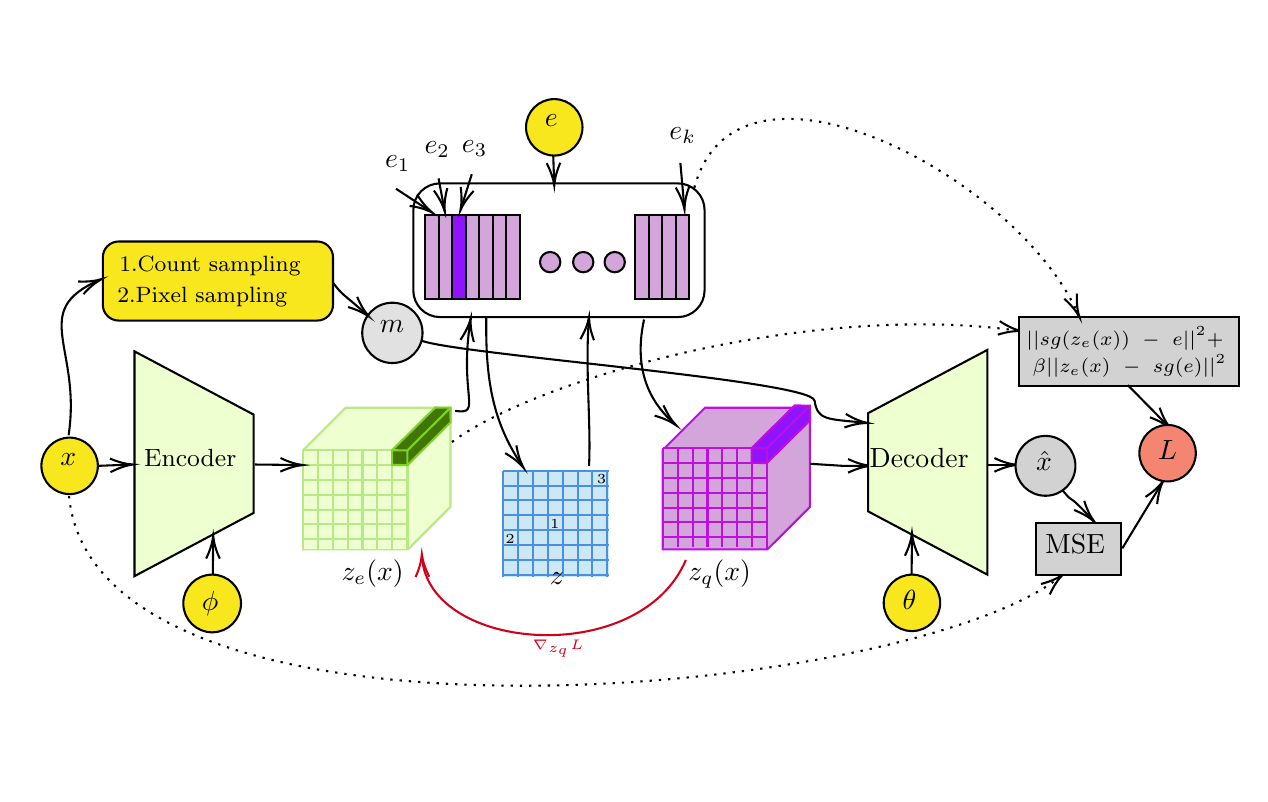
\begin{tikzpicture}[x=0.75pt,y=0.75pt,yscale=-1,xscale=1]
%uncomment if require: \path (0,308); %set diagram left start at 0, and has height of 308

%Shape: Trapezoid [id:dp6171005453979647] 
\draw  [fill={rgb, 255:red, 238; green, 255; blue, 208 }  ,fill opacity=1 ] (107.75,142.44) -- (165.17,172.91) -- (165.17,220.26) -- (107.75,250.73) -- cycle ;
%Shape: Cube [id:dp24555481618180852] 
\draw  [color={rgb, 255:red, 184; green, 233; blue, 134 }  ,draw opacity=1 ][fill={rgb, 255:red, 238; green, 255; blue, 208 }  ,fill opacity=1 ] (189,190.06) -- (209.47,169.59) -- (260,169.59) -- (260,217.36) -- (239.53,237.83) -- (189,237.83) -- cycle ; \draw  [color={rgb, 255:red, 184; green, 233; blue, 134 }  ,draw opacity=1 ] (260,169.59) -- (239.53,190.06) -- (189,190.06) ; \draw  [color={rgb, 255:red, 184; green, 233; blue, 134 }  ,draw opacity=1 ] (239.53,190.06) -- (239.53,237.83) ;
%Shape: Grid [id:dp05381914789010611] 
\draw  [draw opacity=0][fill={rgb, 255:red, 238; green, 255; blue, 208 }  ,fill opacity=1 ][line width=0.75]  (189,190.06) -- (239.36,190.06) -- (239.36,237.83) -- (189,237.83) -- cycle ; \draw  [color={rgb, 255:red, 184; green, 233; blue, 134 }  ,draw opacity=1 ][line width=0.75]  (189,190.06) -- (189,237.83)(196.15,190.06) -- (196.15,237.83)(203.3,190.06) -- (203.3,237.83)(210.45,190.06) -- (210.45,237.83)(217.6,190.06) -- (217.6,237.83)(224.75,190.06) -- (224.75,237.83)(231.9,190.06) -- (231.9,237.83)(239.05,190.06) -- (239.05,237.83) ; \draw  [color={rgb, 255:red, 184; green, 233; blue, 134 }  ,draw opacity=1 ][line width=0.75]  (189,190.06) -- (239.36,190.06)(189,197.21) -- (239.36,197.21)(189,204.36) -- (239.36,204.36)(189,211.51) -- (239.36,211.51)(189,218.66) -- (239.36,218.66)(189,225.81) -- (239.36,225.81)(189,232.96) -- (239.36,232.96) ; \draw  [color={rgb, 255:red, 184; green, 233; blue, 134 }  ,draw opacity=1 ][line width=0.75]   ;
%Shape: Cube [id:dp8396400730940647] 
\draw  [color={rgb, 255:red, 126; green, 211; blue, 33 }  ,draw opacity=1 ][fill={rgb, 255:red, 65; green, 117; blue, 5 }  ,fill opacity=1 ] (231.89,190.05) -- (252.68,169.48) -- (260,169.59) -- (260.03,176.67) -- (239.25,197.24) -- (231.92,197.13) -- cycle ; \draw  [color={rgb, 255:red, 126; green, 211; blue, 33 }  ,draw opacity=1 ] (260,169.59) -- (239.22,190.16) -- (231.89,190.05) ; \draw  [color={rgb, 255:red, 126; green, 211; blue, 33 }  ,draw opacity=1 ] (239.22,190.16) -- (239.25,197.24) ;
%Shape: Grid [id:dp515003631947918] 
\draw  [draw opacity=0][fill={rgb, 255:red, 204; green, 232; blue, 244 }  ,fill opacity=1 ][line width=0.75]  (285.5,199.95) -- (336.5,199.95) -- (336.5,250.95) -- (285.5,250.95) -- cycle ; \draw  [color={rgb, 255:red, 74; green, 144; blue, 226 }  ,draw opacity=1 ][line width=0.75]  (285.5,199.95) -- (285.5,250.95)(292.65,199.95) -- (292.65,250.95)(299.8,199.95) -- (299.8,250.95)(306.95,199.95) -- (306.95,250.95)(314.1,199.95) -- (314.1,250.95)(321.25,199.95) -- (321.25,250.95)(328.4,199.95) -- (328.4,250.95)(335.55,199.95) -- (335.55,250.95) ; \draw  [color={rgb, 255:red, 74; green, 144; blue, 226 }  ,draw opacity=1 ][line width=0.75]  (285.5,199.95) -- (336.5,199.95)(285.5,207.1) -- (336.5,207.1)(285.5,214.25) -- (336.5,214.25)(285.5,221.4) -- (336.5,221.4)(285.5,228.55) -- (336.5,228.55)(285.5,235.7) -- (336.5,235.7)(285.5,242.85) -- (336.5,242.85)(285.5,250) -- (336.5,250) ; \draw  [color={rgb, 255:red, 74; green, 144; blue, 226 }  ,draw opacity=1 ][line width=0.75]   ;
%Shape: Cube [id:dp12345889180485203] 
\draw  [color={rgb, 255:red, 189; green, 16; blue, 224 }  ,draw opacity=1 ][fill={rgb, 255:red, 212; green, 165; blue, 219 }  ,fill opacity=1 ] (362.17,190.06) -- (382.64,169.59) -- (433.17,169.59) -- (433.17,217.36) -- (412.69,237.83) -- (362.17,237.83) -- cycle ; \draw  [color={rgb, 255:red, 189; green, 16; blue, 224 }  ,draw opacity=1 ] (433.17,169.59) -- (412.69,190.06) -- (362.17,190.06) ; \draw  [color={rgb, 255:red, 189; green, 16; blue, 224 }  ,draw opacity=1 ] (412.69,190.06) -- (412.69,237.83) ;
%Shape: Grid [id:dp29312601668778293] 
\draw  [draw opacity=0][fill={rgb, 255:red, 212; green, 165; blue, 219 }  ,fill opacity=1 ][line width=0.75]  (362.37,189.11) -- (412.73,189.11) -- (412.73,236.88) -- (362.37,236.88) -- cycle ; \draw  [color={rgb, 255:red, 189; green, 16; blue, 224 }  ,draw opacity=1 ][line width=0.75]  (362.37,189.11) -- (362.37,236.88)(369.52,189.11) -- (369.52,236.88)(376.67,189.11) -- (376.67,236.88)(383.82,189.11) -- (383.82,236.88)(390.97,189.11) -- (390.97,236.88)(398.12,189.11) -- (398.12,236.88)(405.27,189.11) -- (405.27,236.88)(412.42,189.11) -- (412.42,236.88) ; \draw  [color={rgb, 255:red, 189; green, 16; blue, 224 }  ,draw opacity=1 ][line width=0.75]  (362.37,189.11) -- (412.73,189.11)(362.37,196.26) -- (412.73,196.26)(362.37,203.41) -- (412.73,203.41)(362.37,210.56) -- (412.73,210.56)(362.37,217.71) -- (412.73,217.71)(362.37,224.86) -- (412.73,224.86)(362.37,232.01) -- (412.73,232.01) ; \draw  [color={rgb, 255:red, 189; green, 16; blue, 224 }  ,draw opacity=1 ][line width=0.75]   ;
%Rounded Rect [id:dp41948813884645475] 
\draw   (242.08,74.38) .. controls (242.08,67.27) and (247.85,61.5) .. (254.97,61.5) -- (369.53,61.5) .. controls (376.65,61.5) and (382.42,67.27) .. (382.42,74.38) -- (382.42,113.03) .. controls (382.42,120.15) and (376.65,125.92) .. (369.53,125.92) -- (254.97,125.92) .. controls (247.85,125.92) and (242.08,120.15) .. (242.08,113.03) -- cycle ;
%Shape: Rectangle [id:dp3814163730185258] 
\draw  [fill={rgb, 255:red, 212; green, 165; blue, 219 }  ,fill opacity=1 ] (247.83,76.83) -- (254.33,76.83) -- (254.33,117) -- (247.83,117) -- cycle ;
%Shape: Rectangle [id:dp6795246586501498] 
\draw  [fill={rgb, 255:red, 212; green, 165; blue, 219 }  ,fill opacity=1 ] (254.33,76.83) -- (260.83,76.83) -- (260.83,117) -- (254.33,117) -- cycle ;
%Shape: Rectangle [id:dp7360239293604773] 
\draw  [fill={rgb, 255:red, 144; green, 19; blue, 254 }  ,fill opacity=1 ] (260.83,76.83) -- (267.33,76.83) -- (267.33,117) -- (260.83,117) -- cycle ;
%Shape: Rectangle [id:dp03496075272660548] 
\draw  [fill={rgb, 255:red, 212; green, 165; blue, 219 }  ,fill opacity=1 ] (267.33,76.83) -- (273.83,76.83) -- (273.83,117) -- (267.33,117) -- cycle ;
%Shape: Rectangle [id:dp5808820576420952] 
\draw  [fill={rgb, 255:red, 212; green, 165; blue, 219 }  ,fill opacity=1 ] (273.83,76.83) -- (280.33,76.83) -- (280.33,117) -- (273.83,117) -- cycle ;
%Shape: Rectangle [id:dp5502212726285309] 
\draw  [fill={rgb, 255:red, 212; green, 165; blue, 219 }  ,fill opacity=1 ] (280.33,76.83) -- (286.83,76.83) -- (286.83,117) -- (280.33,117) -- cycle ;
%Shape: Rectangle [id:dp8418323199476655] 
\draw  [fill={rgb, 255:red, 212; green, 165; blue, 219 }  ,fill opacity=1 ] (286.83,76.83) -- (293.33,76.83) -- (293.33,117) -- (286.83,117) -- cycle ;
%Shape: Rectangle [id:dp762117326111954] 
\draw  [fill={rgb, 255:red, 212; green, 165; blue, 219 }  ,fill opacity=1 ] (349,76.83) -- (355.5,76.83) -- (355.5,117) -- (349,117) -- cycle ;
%Shape: Rectangle [id:dp07368895010258736] 
\draw  [fill={rgb, 255:red, 212; green, 165; blue, 219 }  ,fill opacity=1 ] (355.5,76.83) -- (362,76.83) -- (362,117) -- (355.5,117) -- cycle ;
%Shape: Rectangle [id:dp8086354991777767] 
\draw  [fill={rgb, 255:red, 212; green, 165; blue, 219 }  ,fill opacity=1 ] (362,76.83) -- (368.5,76.83) -- (368.5,117) -- (362,117) -- cycle ;
%Shape: Rectangle [id:dp5312315305479934] 
\draw  [fill={rgb, 255:red, 212; green, 165; blue, 219 }  ,fill opacity=1 ] (368.5,76.83) -- (375,76.83) -- (375,117) -- (368.5,117) -- cycle ;
%Shape: Circle [id:dp45438568173773586] 
\draw  [fill={rgb, 255:red, 212; green, 165; blue, 219 }  ,fill opacity=1 ] (319.06,99.44) .. controls (319.06,96.73) and (321.25,94.54) .. (323.96,94.54) .. controls (326.66,94.54) and (328.85,96.73) .. (328.85,99.44) .. controls (328.85,102.14) and (326.66,104.33) .. (323.96,104.33) .. controls (321.25,104.33) and (319.06,102.14) .. (319.06,99.44) -- cycle ;
%Shape: Circle [id:dp972526703594091] 
\draw  [fill={rgb, 255:red, 212; green, 165; blue, 219 }  ,fill opacity=1 ] (334.23,99.44) .. controls (334.23,96.73) and (336.42,94.54) .. (339.12,94.54) .. controls (341.83,94.54) and (344.02,96.73) .. (344.02,99.44) .. controls (344.02,102.14) and (341.83,104.33) .. (339.12,104.33) .. controls (336.42,104.33) and (334.23,102.14) .. (334.23,99.44) -- cycle ;
%Shape: Circle [id:dp1470911418998766] 
\draw  [fill={rgb, 255:red, 212; green, 165; blue, 219 }  ,fill opacity=1 ] (303.12,99.44) .. controls (303.12,96.73) and (305.31,94.54) .. (308.02,94.54) .. controls (310.72,94.54) and (312.92,96.73) .. (312.92,99.44) .. controls (312.92,102.14) and (310.72,104.33) .. (308.02,104.33) .. controls (305.31,104.33) and (303.12,102.14) .. (303.12,99.44) -- cycle ;
%Straight Lines [id:da49701684983766325] 
\draw    (233.75,64.09) -- (249.58,74.49) ;
\draw [shift={(251.25,75.59)}, rotate = 213.31] [color={rgb, 255:red, 0; green, 0; blue, 0 }  ][line width=0.75]    (10.93,-3.29) .. controls (6.95,-1.4) and (3.31,-0.3) .. (0,0) .. controls (3.31,0.3) and (6.95,1.4) .. (10.93,3.29)   ;
%Straight Lines [id:da40432961173063775] 
\draw    (254.25,59.09) -- (256.88,73.12) ;
\draw [shift={(257.25,75.09)}, rotate = 259.38] [color={rgb, 255:red, 0; green, 0; blue, 0 }  ][line width=0.75]    (10.93,-3.29) .. controls (6.95,-1.4) and (3.31,-0.3) .. (0,0) .. controls (3.31,0.3) and (6.95,1.4) .. (10.93,3.29)   ;
%Straight Lines [id:da30890755230557265] 
\draw    (270.25,57.09) -- (265.35,72.68) ;
\draw [shift={(264.75,74.59)}, rotate = 287.45] [color={rgb, 255:red, 0; green, 0; blue, 0 }  ][line width=0.75]    (10.93,-3.29) .. controls (6.95,-1.4) and (3.31,-0.3) .. (0,0) .. controls (3.31,0.3) and (6.95,1.4) .. (10.93,3.29)   ;
%Straight Lines [id:da5228601691518593] 
\draw    (370.75,51.59) -- (372.57,72.09) ;
\draw [shift={(372.75,74.09)}, rotate = 264.92] [color={rgb, 255:red, 0; green, 0; blue, 0 }  ][line width=0.75]    (10.93,-3.29) .. controls (6.95,-1.4) and (3.31,-0.3) .. (0,0) .. controls (3.31,0.3) and (6.95,1.4) .. (10.93,3.29)   ;
%Shape: Cube [id:dp09467921956850145] 
\draw  [color={rgb, 255:red, 189; green, 16; blue, 224 }  ,draw opacity=1 ][fill={rgb, 255:red, 144; green, 19; blue, 254 }  ,fill opacity=1 ] (405.07,189.06) -- (425.85,168.49) -- (433.18,168.6) -- (433.21,175.69) -- (412.42,196.26) -- (405.1,196.15) -- cycle ; \draw  [color={rgb, 255:red, 189; green, 16; blue, 224 }  ,draw opacity=1 ] (433.18,168.6) -- (412.39,189.17) -- (405.07,189.06) ; \draw  [color={rgb, 255:red, 189; green, 16; blue, 224 }  ,draw opacity=1 ] (412.39,189.17) -- (412.42,196.26) ;
%Straight Lines [id:da571391307561518] 
\draw    (433.25,196.59) -- (449,197.59) -- (460.5,197.59) ;
\draw [shift={(462.5,197.59)}, rotate = 180] [color={rgb, 255:red, 0; green, 0; blue, 0 }  ][line width=0.75]    (10.93,-3.29) .. controls (6.95,-1.4) and (3.31,-0.3) .. (0,0) .. controls (3.31,0.3) and (6.95,1.4) .. (10.93,3.29)   ;
%Straight Lines [id:da4813252856254673] 
\draw    (165.8,196.95) -- (187,197.19) ;
\draw [shift={(189,197.21)}, rotate = 180.65] [color={rgb, 255:red, 0; green, 0; blue, 0 }  ][line width=0.75]    (10.93,-3.29) .. controls (6.95,-1.4) and (3.31,-0.3) .. (0,0) .. controls (3.31,0.3) and (6.95,1.4) .. (10.93,3.29)   ;
%Curve Lines [id:da24185321193801135] 
\draw    (277.25,125.92) .. controls (276.76,156.63) and (280.55,176.57) .. (294.18,197.01) ;
\draw [shift={(295.25,198.59)}, rotate = 235.38] [color={rgb, 255:red, 0; green, 0; blue, 0 }  ][line width=0.75]    (10.93,-3.29) .. controls (6.95,-1.4) and (3.31,-0.3) .. (0,0) .. controls (3.31,0.3) and (6.95,1.4) .. (10.93,3.29)   ;
%Curve Lines [id:da6175481636492389] 
\draw    (262.25,171.09) .. controls (275.55,173.06) and (264.1,164.35) .. (269.49,128.25) ;
\draw [shift={(269.75,126.59)}, rotate = 99.09] [color={rgb, 255:red, 0; green, 0; blue, 0 }  ][line width=0.75]    (10.93,-3.29) .. controls (6.95,-1.4) and (3.31,-0.3) .. (0,0) .. controls (3.31,0.3) and (6.95,1.4) .. (10.93,3.29)   ;
%Curve Lines [id:da0945552976420565] 
\draw    (326.75,197.59) .. controls (327.73,177.11) and (324.9,151.72) .. (326.61,127.76) ;
\draw [shift={(326.75,125.92)}, rotate = 94.67] [color={rgb, 255:red, 0; green, 0; blue, 0 }  ][line width=0.75]    (10.93,-3.29) .. controls (6.95,-1.4) and (3.31,-0.3) .. (0,0) .. controls (3.31,0.3) and (6.95,1.4) .. (10.93,3.29)   ;
%Curve Lines [id:da061306482588451394] 
\draw    (353.25,127.09) .. controls (347.14,155.29) and (359.59,169.79) .. (367.33,176.83) ;
\draw [shift={(368.75,178.09)}, rotate = 220.91] [color={rgb, 255:red, 0; green, 0; blue, 0 }  ][line width=0.75]    (10.93,-3.29) .. controls (6.95,-1.4) and (3.31,-0.3) .. (0,0) .. controls (3.31,0.3) and (6.95,1.4) .. (10.93,3.29)   ;
%Shape: Trapezoid [id:dp509627057718193] 
\draw  [fill={rgb, 255:red, 238; green, 255; blue, 208 }  ,fill opacity=1 ] (518.67,250) -- (461.25,219.54) -- (461.25,172.18) -- (518.67,141.72) -- cycle ;
%Straight Lines [id:da5513859940333413] 
\draw    (90.2,197.59) -- (105,197.02) ;
\draw [shift={(107,196.95)}, rotate = 177.82] [color={rgb, 255:red, 0; green, 0; blue, 0 }  ][line width=0.75]    (10.93,-3.29) .. controls (6.95,-1.4) and (3.31,-0.3) .. (0,0) .. controls (3.31,0.3) and (6.95,1.4) .. (10.93,3.29)   ;
%Straight Lines [id:da20905783488241259] 
\draw    (145.5,250) -- (145.65,233.34) ;
\draw [shift={(145.67,231.34)}, rotate = 90.51] [color={rgb, 255:red, 0; green, 0; blue, 0 }  ][line width=0.75]    (10.93,-3.29) .. controls (6.95,-1.4) and (3.31,-0.3) .. (0,0) .. controls (3.31,0.3) and (6.95,1.4) .. (10.93,3.29)   ;
%Straight Lines [id:da68402342001126] 
\draw    (482.17,250) -- (482.32,232.01) ;
\draw [shift={(482.33,230.01)}, rotate = 90.48] [color={rgb, 255:red, 0; green, 0; blue, 0 }  ][line width=0.75]    (10.93,-3.29) .. controls (6.95,-1.4) and (3.31,-0.3) .. (0,0) .. controls (3.31,0.3) and (6.95,1.4) .. (10.93,3.29)   ;
%Straight Lines [id:da7454205013757218] 
\draw    (309.5,48.09) -- (309.93,60.59) ;
\draw [shift={(310,62.59)}, rotate = 268.03] [color={rgb, 255:red, 0; green, 0; blue, 0 }  ][line width=0.75]    (10.93,-3.29) .. controls (6.95,-1.4) and (3.31,-0.3) .. (0,0) .. controls (3.31,0.3) and (6.95,1.4) .. (10.93,3.29)   ;
%Straight Lines [id:da22947795724010012] 
\draw    (519,197.13) -- (531,197.13) ;
\draw [shift={(533,197.13)}, rotate = 180] [color={rgb, 255:red, 0; green, 0; blue, 0 }  ][line width=0.75]    (10.93,-3.29) .. controls (6.95,-1.4) and (3.31,-0.3) .. (0,0) .. controls (3.31,0.3) and (6.95,1.4) .. (10.93,3.29)   ;
%Curve Lines [id:da10579134390387823] 
\draw  [dash pattern={on 0.84pt off 2.51pt}]  (76.2,212.15) .. controls (88.94,345.34) and (480.39,309.71) .. (553.92,250.89) ;
\draw [shift={(555,250)}, rotate = 139.98] [color={rgb, 255:red, 0; green, 0; blue, 0 }  ][line width=0.75]    (10.93,-3.29) .. controls (6.95,-1.4) and (3.31,-0.3) .. (0,0) .. controls (3.31,0.3) and (6.95,1.4) .. (10.93,3.29)   ;
%Curve Lines [id:da9968166114060423] 
\draw  [dash pattern={on 0.84pt off 2.51pt}]  (260.75,186.09) .. controls (300.55,156.24) and (431.68,118.39) .. (533.47,132.46) ;
\draw [shift={(535,132.68)}, rotate = 188.18] [color={rgb, 255:red, 0; green, 0; blue, 0 }  ][line width=0.75]    (10.93,-3.29) .. controls (6.95,-1.4) and (3.31,-0.3) .. (0,0) .. controls (3.31,0.3) and (6.95,1.4) .. (10.93,3.29)   ;
%Straight Lines [id:da7747533234738788] 
\draw    (583.67,237.34) -- (602.3,206.64) ;
\draw [shift={(603.33,204.93)}, rotate = 121.24] [color={rgb, 255:red, 0; green, 0; blue, 0 }  ][line width=0.75]    (10.93,-3.29) .. controls (6.95,-1.4) and (3.31,-0.3) .. (0,0) .. controls (3.31,0.3) and (6.95,1.4) .. (10.93,3.29)   ;
%Shape: Rectangle [id:dp9786445493325081] 
\draw  [fill={rgb, 255:red, 210; green, 210; blue, 210 }  ,fill opacity=1 ] (534,125.92) -- (640,125.92) -- (640,158.92) -- (534,158.92) -- cycle ;
%Straight Lines [id:da12155048936577273] 
\draw    (586.33,158.68) -- (605.6,178.28) ;
\draw [shift={(607,179.71)}, rotate = 225.5] [color={rgb, 255:red, 0; green, 0; blue, 0 }  ][line width=0.75]    (10.93,-3.29) .. controls (6.95,-1.4) and (3.31,-0.3) .. (0,0) .. controls (3.31,0.3) and (6.95,1.4) .. (10.93,3.29)   ;
%Curve Lines [id:da6424562077767642] 
\draw  [dash pattern={on 0.84pt off 2.51pt}]  (377.5,63.59) .. controls (397.9,-13.02) and (533.63,58.2) .. (562.57,124.91) ;
\draw [shift={(563,125.92)}, rotate = 247.32] [color={rgb, 255:red, 0; green, 0; blue, 0 }  ][line width=0.75]    (10.93,-3.29) .. controls (6.95,-1.4) and (3.31,-0.3) .. (0,0) .. controls (3.31,0.3) and (6.95,1.4) .. (10.93,3.29)   ;
%Curve Lines [id:da18266449447129862] 
\draw [color={rgb, 255:red, 208; green, 2; blue, 27 }  ,draw opacity=1 ]   (373.4,242.94) .. controls (351.22,295.22) and (249.46,287.51) .. (246.27,241.55) ;
\draw [shift={(246.2,240.14)}, rotate = 88.54] [color={rgb, 255:red, 208; green, 2; blue, 27 }  ,draw opacity=1 ][line width=0.75]    (10.93,-3.29) .. controls (6.95,-1.4) and (3.31,-0.3) .. (0,0) .. controls (3.31,0.3) and (6.95,1.4) .. (10.93,3.29)   ;
%Curve Lines [id:da7502875492022603] 
\draw    (554.33,208.68) .. controls (562.13,218.19) and (554.72,207.89) .. (569.18,223.43) ;
\draw [shift={(570.33,224.68)}, rotate = 227.29] [color={rgb, 255:red, 0; green, 0; blue, 0 }  ][line width=0.75]    (10.93,-3.29) .. controls (6.95,-1.4) and (3.31,-0.3) .. (0,0) .. controls (3.31,0.3) and (6.95,1.4) .. (10.93,3.29)   ;
%Rounded Rect [id:dp4019707898514915] 
\draw  [fill={rgb, 255:red, 248; green, 231; blue, 28 }  ,fill opacity=1 ] (92.5,97.12) .. controls (92.5,92.91) and (95.91,89.5) .. (100.12,89.5) -- (195.78,89.5) .. controls (199.99,89.5) and (203.4,92.91) .. (203.4,97.12) -- (203.4,119.97) .. controls (203.4,124.18) and (199.99,127.59) .. (195.78,127.59) -- (100.12,127.59) .. controls (95.91,127.59) and (92.5,124.18) .. (92.5,119.97) -- cycle ;
%Curve Lines [id:da45573765480324524] 
\draw    (76,182.85) .. controls (82.4,140.74) and (56.79,123.12) .. (90.42,108.27) ;
\draw [shift={(92,107.59)}, rotate = 157.38] [color={rgb, 255:red, 0; green, 0; blue, 0 }  ][line width=0.75]    (10.93,-3.29) .. controls (6.95,-1.4) and (3.31,-0.3) .. (0,0) .. controls (3.31,0.3) and (6.95,1.4) .. (10.93,3.29)   ;
%Curve Lines [id:da21143051398992896] 
\draw    (203.4,109.35) .. controls (208.42,115.91) and (207.48,113.9) .. (219.63,124.69) ;
\draw [shift={(221,125.92)}, rotate = 221.82] [color={rgb, 255:red, 0; green, 0; blue, 0 }  ][line width=0.75]    (10.93,-3.29) .. controls (6.95,-1.4) and (3.31,-0.3) .. (0,0) .. controls (3.31,0.3) and (6.95,1.4) .. (10.93,3.29)   ;
%Curve Lines [id:da40140404073767766] 
\draw    (246.2,137.35) .. controls (265.4,144.15) and (433.92,156.43) .. (435.4,166.15) .. controls (436.83,175.57) and (441.13,174.99) .. (459.28,176.77) ;
\draw [shift={(461,176.95)}, rotate = 185.83] [color={rgb, 255:red, 0; green, 0; blue, 0 }  ][line width=0.75]    (10.93,-3.29) .. controls (6.95,-1.4) and (3.31,-0.3) .. (0,0) .. controls (3.31,0.3) and (6.95,1.4) .. (10.93,3.29)   ;

% Text Node
\draw (206,241.4) node [anchor=north west][inner sep=0.75pt]    {$z_{e}( x)$};
% Text Node
\draw (373.17,241.4) node [anchor=north west][inner sep=0.75pt]    {$z_{q}( x)$};
% Text Node
\draw (227,46.4) node [anchor=north west][inner sep=0.75pt]    {$e_{1}$};
% Text Node
\draw (246,39.9) node [anchor=north west][inner sep=0.75pt]    {$e_{2}$};
% Text Node
\draw (264,39.4) node [anchor=north west][inner sep=0.75pt]    {$e_{3}$};
% Text Node
\draw (364,32.9) node [anchor=north west][inner sep=0.75pt]    {$e_{k}$};
% Text Node
\draw (329,200.4) node [anchor=north west][inner sep=0.75pt]  [font=\tiny]  {$3$};
% Text Node
\draw (110.9,188.09) node [anchor=north west][inner sep=0.75pt]   [align=left] {{\small Encoder}};
% Text Node
\draw (460.5,187.5) node [anchor=north west][inner sep=0.75pt]   [align=left] {Decoder};
% Text Node
\draw  [fill={rgb, 255:red, 248; green, 231; blue, 28 }  ,fill opacity=1 ]  (145.17, 263.9) circle [x radius= 13.9, y radius= 13.9]   ;
\draw (138.67,256.3) node [anchor=north west][inner sep=0.75pt]  [font=\normalsize]  {$\phi $};
% Text Node
\draw  [fill={rgb, 255:red, 248; green, 231; blue, 28 }  ,fill opacity=1 ]  (482.33, 263.6) circle [x radius= 13.6, y radius= 13.6]   ;
\draw (476.33,256) node [anchor=north west][inner sep=0.75pt]  [font=\normalsize]  {$\theta $};
% Text Node
\draw  [fill={rgb, 255:red, 248; green, 231; blue, 28 }  ,fill opacity=1 ]  (76.5, 197.59) circle [x radius= 13.6, y radius= 13.6]   ;
\draw (70.5,189.99) node [anchor=north west][inner sep=0.75pt]  [font=\normalsize]  {$x$};
% Text Node
\draw  [fill={rgb, 255:red, 210; green, 210; blue, 210 }  ,fill opacity=1 ]  (546.67, 197.59) circle [x radius= 14.42, y radius= 14.42]   ;
\draw (540.67,188.99) node [anchor=north west][inner sep=0.75pt]  [font=\normalsize]  {$\hat{x}$};
% Text Node
\draw  [fill={rgb, 255:red, 248; green, 231; blue, 28 }  ,fill opacity=1 ]  (310, 34.5) circle [x radius= 13.6, y radius= 13.6]   ;
\draw (304,26.9) node [anchor=north west][inner sep=0.75pt]  [font=\normalsize]  {$e$};
% Text Node
\draw  [fill={rgb, 255:red, 210; green, 210; blue, 210 }  ,fill opacity=1 ]  (542.17,225) -- (583.17,225) -- (583.17,250) -- (542.17,250) -- cycle  ;
\draw (545.17,229) node [anchor=north west][inner sep=0.75pt]   [align=left] {MSE};
% Text Node
\draw  [fill={rgb, 255:red, 244; green, 134; blue, 113 }  ,fill opacity=1 ]  (605.5, 191.5) circle [x radius= 13.6, y radius= 13.6]   ;
\draw (599.5,183.9) node [anchor=north west][inner sep=0.75pt]    {$L$};
% Text Node
\draw (306.5,221.9) node [anchor=north west][inner sep=0.75pt]  [font=\tiny]  {$1$};
% Text Node
\draw (285,229.06) node [anchor=north west][inner sep=0.75pt]  [font=\tiny]  {$2$};
% Text Node
\draw (536,128.92) node [anchor=north west][inner sep=0.75pt]  [font=\scriptsize] [align=left] {$\displaystyle ||sg( z_{e}( x)) \ -\ e||^{2} +$};
% Text Node
\draw (539,142.33) node [anchor=north west][inner sep=0.75pt]  [font=\scriptsize] [align=left] {$\displaystyle \beta ||z_{e}( x) \ -\ sg( e) ||^{2}$};
% Text Node
\draw (306.4,247.6) node [anchor=north west][inner sep=0.75pt]    {$z$};
% Text Node
\draw (298,279.94) node [anchor=north west][inner sep=0.75pt]  [font=\tiny,color={rgb, 255:red, 208; green, 2; blue, 27 }  ,opacity=1 ]  {$\nabla _{z_{q}} L$};
% Text Node
\draw  [fill={rgb, 255:red, 155; green, 155; blue, 155 }  ,fill opacity=0.3 ]  (232, 133.52) circle [x radius= 14.53, y radius= 14.53]   ;
\draw (224.5,125.92) node [anchor=north west][inner sep=0.75pt]  [font=\normalsize]  {$m$};
% Text Node
\draw (99,95) node [anchor=north west][inner sep=0.75pt]  [font=\footnotesize] [align=left] {1.Count sampling};
% Text Node
\draw (98,110) node [anchor=north west][inner sep=0.75pt]  [font=\footnotesize] [align=left] {2.Pixel sampling};


\end{tikzpicture}

    \caption{Cross-validation results of \methodTwo{2} applied to a VQ-VAE(Config. Nr. 3) on the CelebA dataset.}
    \label{tab:results_method2_vq_vae}
\end{table}
\begin{figure}[H]
    \centering
    \scalebox{0.48}{%% Creator: Matplotlib, PGF backend
%%
%% To include the figure in your LaTeX document, write
%%   \input{<filename>.pgf}
%%
%% Make sure the required packages are loaded in your preamble
%%   \usepackage{pgf}
%%
%% Also ensure that all the required font packages are loaded; for instance,
%% the lmodern package is sometimes necessary when using math font.
%%   \usepackage{lmodern}
%%
%% Figures using additional raster images can only be included by \input if
%% they are in the same directory as the main LaTeX file. For loading figures
%% from other directories you can use the `import` package
%%   \usepackage{import}
%%
%% and then include the figures with
%%   \import{<path to file>}{<filename>.pgf}
%%
%% Matplotlib used the following preamble
%%   
%%   \usepackage{fontspec}
%%   \setmainfont{DejaVuSerif.ttf}[Path=\detokenize{/home/edvardsz/miniconda3/envs/pytorch-latest/lib/python3.10/site-packages/matplotlib/mpl-data/fonts/ttf/}]
%%   \setsansfont{DejaVuSans.ttf}[Path=\detokenize{/home/edvardsz/miniconda3/envs/pytorch-latest/lib/python3.10/site-packages/matplotlib/mpl-data/fonts/ttf/}]
%%   \setmonofont{DejaVuSansMono.ttf}[Path=\detokenize{/home/edvardsz/miniconda3/envs/pytorch-latest/lib/python3.10/site-packages/matplotlib/mpl-data/fonts/ttf/}]
%%   \makeatletter\@ifpackageloaded{underscore}{}{\usepackage[strings]{underscore}}\makeatother
%%
\begingroup%
\makeatletter%
\begin{pgfpicture}%
\pgfpathrectangle{\pgfpointorigin}{\pgfqpoint{6.400000in}{4.800000in}}%
\pgfusepath{use as bounding box, clip}%
\begin{pgfscope}%
\pgfsetbuttcap%
\pgfsetmiterjoin%
\definecolor{currentfill}{rgb}{1.000000,1.000000,1.000000}%
\pgfsetfillcolor{currentfill}%
\pgfsetlinewidth{0.000000pt}%
\definecolor{currentstroke}{rgb}{1.000000,1.000000,1.000000}%
\pgfsetstrokecolor{currentstroke}%
\pgfsetdash{}{0pt}%
\pgfpathmoveto{\pgfqpoint{0.000000in}{0.000000in}}%
\pgfpathlineto{\pgfqpoint{6.400000in}{0.000000in}}%
\pgfpathlineto{\pgfqpoint{6.400000in}{4.800000in}}%
\pgfpathlineto{\pgfqpoint{0.000000in}{4.800000in}}%
\pgfpathlineto{\pgfqpoint{0.000000in}{0.000000in}}%
\pgfpathclose%
\pgfusepath{fill}%
\end{pgfscope}%
\begin{pgfscope}%
\pgfsetbuttcap%
\pgfsetmiterjoin%
\definecolor{currentfill}{rgb}{1.000000,1.000000,1.000000}%
\pgfsetfillcolor{currentfill}%
\pgfsetlinewidth{0.000000pt}%
\definecolor{currentstroke}{rgb}{0.000000,0.000000,0.000000}%
\pgfsetstrokecolor{currentstroke}%
\pgfsetstrokeopacity{0.000000}%
\pgfsetdash{}{0pt}%
\pgfpathmoveto{\pgfqpoint{0.800000in}{0.528000in}}%
\pgfpathlineto{\pgfqpoint{5.760000in}{0.528000in}}%
\pgfpathlineto{\pgfqpoint{5.760000in}{4.224000in}}%
\pgfpathlineto{\pgfqpoint{0.800000in}{4.224000in}}%
\pgfpathlineto{\pgfqpoint{0.800000in}{0.528000in}}%
\pgfpathclose%
\pgfusepath{fill}%
\end{pgfscope}%
\begin{pgfscope}%
\pgfpathrectangle{\pgfqpoint{0.800000in}{0.528000in}}{\pgfqpoint{4.960000in}{3.696000in}}%
\pgfusepath{clip}%
\pgfsetbuttcap%
\pgfsetroundjoin%
\definecolor{currentfill}{rgb}{0.121569,0.466667,0.705882}%
\pgfsetfillcolor{currentfill}%
\pgfsetfillopacity{0.200000}%
\pgfsetlinewidth{0.000000pt}%
\definecolor{currentstroke}{rgb}{0.000000,0.000000,0.000000}%
\pgfsetstrokecolor{currentstroke}%
\pgfsetdash{}{0pt}%
\pgfpathmoveto{\pgfqpoint{1.025455in}{2.860737in}}%
\pgfpathlineto{\pgfqpoint{1.025455in}{1.723409in}}%
\pgfpathlineto{\pgfqpoint{1.072919in}{1.649044in}}%
\pgfpathlineto{\pgfqpoint{1.120383in}{1.649606in}}%
\pgfpathlineto{\pgfqpoint{1.167847in}{1.816119in}}%
\pgfpathlineto{\pgfqpoint{1.215311in}{1.471003in}}%
\pgfpathlineto{\pgfqpoint{1.262775in}{1.505466in}}%
\pgfpathlineto{\pgfqpoint{1.310239in}{1.420618in}}%
\pgfpathlineto{\pgfqpoint{1.357703in}{1.348253in}}%
\pgfpathlineto{\pgfqpoint{1.405167in}{1.334373in}}%
\pgfpathlineto{\pgfqpoint{1.452632in}{1.203436in}}%
\pgfpathlineto{\pgfqpoint{1.500096in}{1.260909in}}%
\pgfpathlineto{\pgfqpoint{1.547560in}{1.176695in}}%
\pgfpathlineto{\pgfqpoint{1.595024in}{1.213403in}}%
\pgfpathlineto{\pgfqpoint{1.642488in}{1.209940in}}%
\pgfpathlineto{\pgfqpoint{1.689952in}{1.183093in}}%
\pgfpathlineto{\pgfqpoint{1.737416in}{1.188741in}}%
\pgfpathlineto{\pgfqpoint{1.784880in}{1.110832in}}%
\pgfpathlineto{\pgfqpoint{1.832344in}{1.255096in}}%
\pgfpathlineto{\pgfqpoint{1.879809in}{1.181001in}}%
\pgfpathlineto{\pgfqpoint{1.927273in}{1.131461in}}%
\pgfpathlineto{\pgfqpoint{1.974737in}{1.080482in}}%
\pgfpathlineto{\pgfqpoint{2.022201in}{1.070444in}}%
\pgfpathlineto{\pgfqpoint{2.069665in}{1.121680in}}%
\pgfpathlineto{\pgfqpoint{2.117129in}{1.224879in}}%
\pgfpathlineto{\pgfqpoint{2.164593in}{1.126229in}}%
\pgfpathlineto{\pgfqpoint{2.212057in}{1.131400in}}%
\pgfpathlineto{\pgfqpoint{2.259522in}{1.096647in}}%
\pgfpathlineto{\pgfqpoint{2.306986in}{1.145366in}}%
\pgfpathlineto{\pgfqpoint{2.354450in}{1.187535in}}%
\pgfpathlineto{\pgfqpoint{2.401914in}{1.076182in}}%
\pgfpathlineto{\pgfqpoint{2.449378in}{1.067341in}}%
\pgfpathlineto{\pgfqpoint{2.496842in}{1.042669in}}%
\pgfpathlineto{\pgfqpoint{2.544306in}{1.062502in}}%
\pgfpathlineto{\pgfqpoint{2.591770in}{1.069743in}}%
\pgfpathlineto{\pgfqpoint{2.639234in}{1.061588in}}%
\pgfpathlineto{\pgfqpoint{2.686699in}{1.011974in}}%
\pgfpathlineto{\pgfqpoint{2.734163in}{1.015045in}}%
\pgfpathlineto{\pgfqpoint{2.781627in}{1.005460in}}%
\pgfpathlineto{\pgfqpoint{2.829091in}{0.992018in}}%
\pgfpathlineto{\pgfqpoint{2.876555in}{0.994254in}}%
\pgfpathlineto{\pgfqpoint{2.924019in}{0.961880in}}%
\pgfpathlineto{\pgfqpoint{2.971483in}{0.962949in}}%
\pgfpathlineto{\pgfqpoint{3.018947in}{0.948292in}}%
\pgfpathlineto{\pgfqpoint{3.066411in}{0.946684in}}%
\pgfpathlineto{\pgfqpoint{3.113876in}{0.972913in}}%
\pgfpathlineto{\pgfqpoint{3.161340in}{0.940505in}}%
\pgfpathlineto{\pgfqpoint{3.208804in}{0.963111in}}%
\pgfpathlineto{\pgfqpoint{3.256268in}{0.939040in}}%
\pgfpathlineto{\pgfqpoint{3.303732in}{0.914598in}}%
\pgfpathlineto{\pgfqpoint{3.351196in}{0.900604in}}%
\pgfpathlineto{\pgfqpoint{3.398660in}{0.897304in}}%
\pgfpathlineto{\pgfqpoint{3.446124in}{0.908442in}}%
\pgfpathlineto{\pgfqpoint{3.493589in}{0.906977in}}%
\pgfpathlineto{\pgfqpoint{3.541053in}{0.900501in}}%
\pgfpathlineto{\pgfqpoint{3.588517in}{0.898282in}}%
\pgfpathlineto{\pgfqpoint{3.635981in}{0.877757in}}%
\pgfpathlineto{\pgfqpoint{3.683445in}{0.895300in}}%
\pgfpathlineto{\pgfqpoint{3.730909in}{0.876546in}}%
\pgfpathlineto{\pgfqpoint{3.778373in}{0.856965in}}%
\pgfpathlineto{\pgfqpoint{3.825837in}{0.836466in}}%
\pgfpathlineto{\pgfqpoint{3.873301in}{0.871280in}}%
\pgfpathlineto{\pgfqpoint{3.920766in}{0.847772in}}%
\pgfpathlineto{\pgfqpoint{3.968230in}{0.833736in}}%
\pgfpathlineto{\pgfqpoint{4.015694in}{0.837937in}}%
\pgfpathlineto{\pgfqpoint{4.063158in}{0.826138in}}%
\pgfpathlineto{\pgfqpoint{4.110622in}{0.806844in}}%
\pgfpathlineto{\pgfqpoint{4.158086in}{0.827047in}}%
\pgfpathlineto{\pgfqpoint{4.205550in}{0.836322in}}%
\pgfpathlineto{\pgfqpoint{4.253014in}{0.810749in}}%
\pgfpathlineto{\pgfqpoint{4.300478in}{0.805406in}}%
\pgfpathlineto{\pgfqpoint{4.347943in}{0.790330in}}%
\pgfpathlineto{\pgfqpoint{4.395407in}{0.791387in}}%
\pgfpathlineto{\pgfqpoint{4.442871in}{0.791084in}}%
\pgfpathlineto{\pgfqpoint{4.490335in}{0.767829in}}%
\pgfpathlineto{\pgfqpoint{4.537799in}{0.771266in}}%
\pgfpathlineto{\pgfqpoint{4.585263in}{0.762725in}}%
\pgfpathlineto{\pgfqpoint{4.632727in}{0.740555in}}%
\pgfpathlineto{\pgfqpoint{4.680191in}{0.775323in}}%
\pgfpathlineto{\pgfqpoint{4.727656in}{0.754338in}}%
\pgfpathlineto{\pgfqpoint{4.775120in}{0.760984in}}%
\pgfpathlineto{\pgfqpoint{4.822584in}{0.757244in}}%
\pgfpathlineto{\pgfqpoint{4.870048in}{0.775497in}}%
\pgfpathlineto{\pgfqpoint{4.917512in}{0.769251in}}%
\pgfpathlineto{\pgfqpoint{4.964976in}{0.727985in}}%
\pgfpathlineto{\pgfqpoint{5.012440in}{0.744322in}}%
\pgfpathlineto{\pgfqpoint{5.059904in}{0.722958in}}%
\pgfpathlineto{\pgfqpoint{5.107368in}{0.735935in}}%
\pgfpathlineto{\pgfqpoint{5.154833in}{0.726184in}}%
\pgfpathlineto{\pgfqpoint{5.202297in}{0.716458in}}%
\pgfpathlineto{\pgfqpoint{5.249761in}{0.710542in}}%
\pgfpathlineto{\pgfqpoint{5.297225in}{0.721597in}}%
\pgfpathlineto{\pgfqpoint{5.344689in}{0.729200in}}%
\pgfpathlineto{\pgfqpoint{5.392153in}{0.698974in}}%
\pgfpathlineto{\pgfqpoint{5.439617in}{0.709698in}}%
\pgfpathlineto{\pgfqpoint{5.487081in}{0.707503in}}%
\pgfpathlineto{\pgfqpoint{5.534545in}{0.696000in}}%
\pgfpathlineto{\pgfqpoint{5.534545in}{1.215788in}}%
\pgfpathlineto{\pgfqpoint{5.534545in}{1.215788in}}%
\pgfpathlineto{\pgfqpoint{5.487081in}{1.193857in}}%
\pgfpathlineto{\pgfqpoint{5.439617in}{1.203340in}}%
\pgfpathlineto{\pgfqpoint{5.392153in}{1.203950in}}%
\pgfpathlineto{\pgfqpoint{5.344689in}{1.229506in}}%
\pgfpathlineto{\pgfqpoint{5.297225in}{1.207540in}}%
\pgfpathlineto{\pgfqpoint{5.249761in}{1.246378in}}%
\pgfpathlineto{\pgfqpoint{5.202297in}{1.231804in}}%
\pgfpathlineto{\pgfqpoint{5.154833in}{1.232621in}}%
\pgfpathlineto{\pgfqpoint{5.107368in}{1.223739in}}%
\pgfpathlineto{\pgfqpoint{5.059904in}{1.283657in}}%
\pgfpathlineto{\pgfqpoint{5.012440in}{1.350381in}}%
\pgfpathlineto{\pgfqpoint{4.964976in}{1.290705in}}%
\pgfpathlineto{\pgfqpoint{4.917512in}{1.286399in}}%
\pgfpathlineto{\pgfqpoint{4.870048in}{1.234174in}}%
\pgfpathlineto{\pgfqpoint{4.822584in}{1.278427in}}%
\pgfpathlineto{\pgfqpoint{4.775120in}{1.336186in}}%
\pgfpathlineto{\pgfqpoint{4.727656in}{1.250252in}}%
\pgfpathlineto{\pgfqpoint{4.680191in}{1.277112in}}%
\pgfpathlineto{\pgfqpoint{4.632727in}{1.287056in}}%
\pgfpathlineto{\pgfqpoint{4.585263in}{1.319355in}}%
\pgfpathlineto{\pgfqpoint{4.537799in}{1.333277in}}%
\pgfpathlineto{\pgfqpoint{4.490335in}{1.283381in}}%
\pgfpathlineto{\pgfqpoint{4.442871in}{1.258267in}}%
\pgfpathlineto{\pgfqpoint{4.395407in}{1.342026in}}%
\pgfpathlineto{\pgfqpoint{4.347943in}{1.308938in}}%
\pgfpathlineto{\pgfqpoint{4.300478in}{1.321989in}}%
\pgfpathlineto{\pgfqpoint{4.253014in}{1.232903in}}%
\pgfpathlineto{\pgfqpoint{4.205550in}{1.263499in}}%
\pgfpathlineto{\pgfqpoint{4.158086in}{1.292432in}}%
\pgfpathlineto{\pgfqpoint{4.110622in}{1.300707in}}%
\pgfpathlineto{\pgfqpoint{4.063158in}{1.341470in}}%
\pgfpathlineto{\pgfqpoint{4.015694in}{1.340682in}}%
\pgfpathlineto{\pgfqpoint{3.968230in}{1.294368in}}%
\pgfpathlineto{\pgfqpoint{3.920766in}{1.313864in}}%
\pgfpathlineto{\pgfqpoint{3.873301in}{1.304749in}}%
\pgfpathlineto{\pgfqpoint{3.825837in}{1.298738in}}%
\pgfpathlineto{\pgfqpoint{3.778373in}{1.325100in}}%
\pgfpathlineto{\pgfqpoint{3.730909in}{1.349643in}}%
\pgfpathlineto{\pgfqpoint{3.683445in}{1.316552in}}%
\pgfpathlineto{\pgfqpoint{3.635981in}{1.306196in}}%
\pgfpathlineto{\pgfqpoint{3.588517in}{1.284403in}}%
\pgfpathlineto{\pgfqpoint{3.541053in}{1.331730in}}%
\pgfpathlineto{\pgfqpoint{3.493589in}{1.349702in}}%
\pgfpathlineto{\pgfqpoint{3.446124in}{1.339739in}}%
\pgfpathlineto{\pgfqpoint{3.398660in}{1.337746in}}%
\pgfpathlineto{\pgfqpoint{3.351196in}{1.307244in}}%
\pgfpathlineto{\pgfqpoint{3.303732in}{1.322631in}}%
\pgfpathlineto{\pgfqpoint{3.256268in}{1.342385in}}%
\pgfpathlineto{\pgfqpoint{3.208804in}{1.365419in}}%
\pgfpathlineto{\pgfqpoint{3.161340in}{1.374551in}}%
\pgfpathlineto{\pgfqpoint{3.113876in}{1.400281in}}%
\pgfpathlineto{\pgfqpoint{3.066411in}{1.383748in}}%
\pgfpathlineto{\pgfqpoint{3.018947in}{1.415084in}}%
\pgfpathlineto{\pgfqpoint{2.971483in}{1.397666in}}%
\pgfpathlineto{\pgfqpoint{2.924019in}{1.463772in}}%
\pgfpathlineto{\pgfqpoint{2.876555in}{1.512136in}}%
\pgfpathlineto{\pgfqpoint{2.829091in}{1.506275in}}%
\pgfpathlineto{\pgfqpoint{2.781627in}{1.455796in}}%
\pgfpathlineto{\pgfqpoint{2.734163in}{1.468918in}}%
\pgfpathlineto{\pgfqpoint{2.686699in}{1.581896in}}%
\pgfpathlineto{\pgfqpoint{2.639234in}{1.559123in}}%
\pgfpathlineto{\pgfqpoint{2.591770in}{1.502433in}}%
\pgfpathlineto{\pgfqpoint{2.544306in}{1.473477in}}%
\pgfpathlineto{\pgfqpoint{2.496842in}{1.486697in}}%
\pgfpathlineto{\pgfqpoint{2.449378in}{1.529765in}}%
\pgfpathlineto{\pgfqpoint{2.401914in}{1.578941in}}%
\pgfpathlineto{\pgfqpoint{2.354450in}{1.601219in}}%
\pgfpathlineto{\pgfqpoint{2.306986in}{1.656475in}}%
\pgfpathlineto{\pgfqpoint{2.259522in}{1.789649in}}%
\pgfpathlineto{\pgfqpoint{2.212057in}{1.787936in}}%
\pgfpathlineto{\pgfqpoint{2.164593in}{1.833399in}}%
\pgfpathlineto{\pgfqpoint{2.117129in}{1.904242in}}%
\pgfpathlineto{\pgfqpoint{2.069665in}{1.883464in}}%
\pgfpathlineto{\pgfqpoint{2.022201in}{2.037799in}}%
\pgfpathlineto{\pgfqpoint{1.974737in}{2.122879in}}%
\pgfpathlineto{\pgfqpoint{1.927273in}{2.093140in}}%
\pgfpathlineto{\pgfqpoint{1.879809in}{2.131025in}}%
\pgfpathlineto{\pgfqpoint{1.832344in}{2.127043in}}%
\pgfpathlineto{\pgfqpoint{1.784880in}{2.182864in}}%
\pgfpathlineto{\pgfqpoint{1.737416in}{2.112927in}}%
\pgfpathlineto{\pgfqpoint{1.689952in}{2.226372in}}%
\pgfpathlineto{\pgfqpoint{1.642488in}{2.119406in}}%
\pgfpathlineto{\pgfqpoint{1.595024in}{2.281474in}}%
\pgfpathlineto{\pgfqpoint{1.547560in}{2.144199in}}%
\pgfpathlineto{\pgfqpoint{1.500096in}{2.333543in}}%
\pgfpathlineto{\pgfqpoint{1.452632in}{2.346556in}}%
\pgfpathlineto{\pgfqpoint{1.405167in}{2.506804in}}%
\pgfpathlineto{\pgfqpoint{1.357703in}{2.460083in}}%
\pgfpathlineto{\pgfqpoint{1.310239in}{2.345298in}}%
\pgfpathlineto{\pgfqpoint{1.262775in}{2.412749in}}%
\pgfpathlineto{\pgfqpoint{1.215311in}{2.332053in}}%
\pgfpathlineto{\pgfqpoint{1.167847in}{2.488004in}}%
\pgfpathlineto{\pgfqpoint{1.120383in}{2.604372in}}%
\pgfpathlineto{\pgfqpoint{1.072919in}{2.720299in}}%
\pgfpathlineto{\pgfqpoint{1.025455in}{2.860737in}}%
\pgfpathlineto{\pgfqpoint{1.025455in}{2.860737in}}%
\pgfpathclose%
\pgfusepath{fill}%
\end{pgfscope}%
\begin{pgfscope}%
\pgfpathrectangle{\pgfqpoint{0.800000in}{0.528000in}}{\pgfqpoint{4.960000in}{3.696000in}}%
\pgfusepath{clip}%
\pgfsetbuttcap%
\pgfsetroundjoin%
\definecolor{currentfill}{rgb}{1.000000,0.498039,0.054902}%
\pgfsetfillcolor{currentfill}%
\pgfsetfillopacity{0.200000}%
\pgfsetlinewidth{0.000000pt}%
\definecolor{currentstroke}{rgb}{0.000000,0.000000,0.000000}%
\pgfsetstrokecolor{currentstroke}%
\pgfsetdash{}{0pt}%
\pgfpathmoveto{\pgfqpoint{1.025455in}{4.002615in}}%
\pgfpathlineto{\pgfqpoint{1.025455in}{1.759154in}}%
\pgfpathlineto{\pgfqpoint{1.072919in}{1.801583in}}%
\pgfpathlineto{\pgfqpoint{1.120383in}{1.785909in}}%
\pgfpathlineto{\pgfqpoint{1.167847in}{1.819205in}}%
\pgfpathlineto{\pgfqpoint{1.215311in}{1.775087in}}%
\pgfpathlineto{\pgfqpoint{1.262775in}{1.779284in}}%
\pgfpathlineto{\pgfqpoint{1.310239in}{2.169553in}}%
\pgfpathlineto{\pgfqpoint{1.357703in}{1.892619in}}%
\pgfpathlineto{\pgfqpoint{1.405167in}{1.805328in}}%
\pgfpathlineto{\pgfqpoint{1.452632in}{2.063085in}}%
\pgfpathlineto{\pgfqpoint{1.500096in}{2.229710in}}%
\pgfpathlineto{\pgfqpoint{1.547560in}{2.255939in}}%
\pgfpathlineto{\pgfqpoint{1.595024in}{2.342783in}}%
\pgfpathlineto{\pgfqpoint{1.642488in}{2.476612in}}%
\pgfpathlineto{\pgfqpoint{1.689952in}{2.262209in}}%
\pgfpathlineto{\pgfqpoint{1.737416in}{2.317317in}}%
\pgfpathlineto{\pgfqpoint{1.784880in}{2.349218in}}%
\pgfpathlineto{\pgfqpoint{1.832344in}{2.379939in}}%
\pgfpathlineto{\pgfqpoint{1.879809in}{2.273864in}}%
\pgfpathlineto{\pgfqpoint{1.927273in}{2.363444in}}%
\pgfpathlineto{\pgfqpoint{1.974737in}{2.209144in}}%
\pgfpathlineto{\pgfqpoint{2.022201in}{2.321915in}}%
\pgfpathlineto{\pgfqpoint{2.069665in}{2.259341in}}%
\pgfpathlineto{\pgfqpoint{2.117129in}{2.166783in}}%
\pgfpathlineto{\pgfqpoint{2.164593in}{2.049919in}}%
\pgfpathlineto{\pgfqpoint{2.212057in}{2.106188in}}%
\pgfpathlineto{\pgfqpoint{2.259522in}{2.282648in}}%
\pgfpathlineto{\pgfqpoint{2.306986in}{2.044165in}}%
\pgfpathlineto{\pgfqpoint{2.354450in}{2.174288in}}%
\pgfpathlineto{\pgfqpoint{2.401914in}{1.888150in}}%
\pgfpathlineto{\pgfqpoint{2.449378in}{1.965950in}}%
\pgfpathlineto{\pgfqpoint{2.496842in}{1.977069in}}%
\pgfpathlineto{\pgfqpoint{2.544306in}{1.860460in}}%
\pgfpathlineto{\pgfqpoint{2.591770in}{1.863378in}}%
\pgfpathlineto{\pgfqpoint{2.639234in}{1.843201in}}%
\pgfpathlineto{\pgfqpoint{2.686699in}{1.804632in}}%
\pgfpathlineto{\pgfqpoint{2.734163in}{1.869441in}}%
\pgfpathlineto{\pgfqpoint{2.781627in}{1.870357in}}%
\pgfpathlineto{\pgfqpoint{2.829091in}{1.762381in}}%
\pgfpathlineto{\pgfqpoint{2.876555in}{1.673601in}}%
\pgfpathlineto{\pgfqpoint{2.924019in}{1.520087in}}%
\pgfpathlineto{\pgfqpoint{2.971483in}{1.496878in}}%
\pgfpathlineto{\pgfqpoint{3.018947in}{1.497293in}}%
\pgfpathlineto{\pgfqpoint{3.066411in}{1.432831in}}%
\pgfpathlineto{\pgfqpoint{3.113876in}{1.504002in}}%
\pgfpathlineto{\pgfqpoint{3.161340in}{1.449797in}}%
\pgfpathlineto{\pgfqpoint{3.208804in}{1.440751in}}%
\pgfpathlineto{\pgfqpoint{3.256268in}{1.536005in}}%
\pgfpathlineto{\pgfqpoint{3.303732in}{1.447511in}}%
\pgfpathlineto{\pgfqpoint{3.351196in}{1.425176in}}%
\pgfpathlineto{\pgfqpoint{3.398660in}{1.400495in}}%
\pgfpathlineto{\pgfqpoint{3.446124in}{1.532256in}}%
\pgfpathlineto{\pgfqpoint{3.493589in}{1.413508in}}%
\pgfpathlineto{\pgfqpoint{3.541053in}{1.483139in}}%
\pgfpathlineto{\pgfqpoint{3.588517in}{1.464761in}}%
\pgfpathlineto{\pgfqpoint{3.635981in}{1.257244in}}%
\pgfpathlineto{\pgfqpoint{3.683445in}{1.284992in}}%
\pgfpathlineto{\pgfqpoint{3.730909in}{1.277220in}}%
\pgfpathlineto{\pgfqpoint{3.778373in}{1.250384in}}%
\pgfpathlineto{\pgfqpoint{3.825837in}{1.303873in}}%
\pgfpathlineto{\pgfqpoint{3.873301in}{1.261019in}}%
\pgfpathlineto{\pgfqpoint{3.920766in}{1.228516in}}%
\pgfpathlineto{\pgfqpoint{3.968230in}{1.304399in}}%
\pgfpathlineto{\pgfqpoint{4.015694in}{1.210811in}}%
\pgfpathlineto{\pgfqpoint{4.063158in}{1.279109in}}%
\pgfpathlineto{\pgfqpoint{4.110622in}{1.299076in}}%
\pgfpathlineto{\pgfqpoint{4.158086in}{1.217850in}}%
\pgfpathlineto{\pgfqpoint{4.205550in}{1.263294in}}%
\pgfpathlineto{\pgfqpoint{4.253014in}{1.198158in}}%
\pgfpathlineto{\pgfqpoint{4.300478in}{1.245106in}}%
\pgfpathlineto{\pgfqpoint{4.347943in}{1.216504in}}%
\pgfpathlineto{\pgfqpoint{4.395407in}{1.292649in}}%
\pgfpathlineto{\pgfqpoint{4.442871in}{1.231213in}}%
\pgfpathlineto{\pgfqpoint{4.490335in}{1.220689in}}%
\pgfpathlineto{\pgfqpoint{4.537799in}{1.217323in}}%
\pgfpathlineto{\pgfqpoint{4.585263in}{1.209241in}}%
\pgfpathlineto{\pgfqpoint{4.632727in}{1.192570in}}%
\pgfpathlineto{\pgfqpoint{4.680191in}{1.232403in}}%
\pgfpathlineto{\pgfqpoint{4.727656in}{1.157354in}}%
\pgfpathlineto{\pgfqpoint{4.775120in}{1.180912in}}%
\pgfpathlineto{\pgfqpoint{4.822584in}{1.169007in}}%
\pgfpathlineto{\pgfqpoint{4.870048in}{1.051861in}}%
\pgfpathlineto{\pgfqpoint{4.917512in}{1.116336in}}%
\pgfpathlineto{\pgfqpoint{4.964976in}{1.121446in}}%
\pgfpathlineto{\pgfqpoint{5.012440in}{1.051462in}}%
\pgfpathlineto{\pgfqpoint{5.059904in}{1.087032in}}%
\pgfpathlineto{\pgfqpoint{5.107368in}{1.082935in}}%
\pgfpathlineto{\pgfqpoint{5.154833in}{1.063638in}}%
\pgfpathlineto{\pgfqpoint{5.202297in}{1.111976in}}%
\pgfpathlineto{\pgfqpoint{5.249761in}{1.078678in}}%
\pgfpathlineto{\pgfqpoint{5.297225in}{1.060173in}}%
\pgfpathlineto{\pgfqpoint{5.344689in}{1.059418in}}%
\pgfpathlineto{\pgfqpoint{5.392153in}{1.087448in}}%
\pgfpathlineto{\pgfqpoint{5.439617in}{1.043407in}}%
\pgfpathlineto{\pgfqpoint{5.487081in}{1.087593in}}%
\pgfpathlineto{\pgfqpoint{5.534545in}{1.088356in}}%
\pgfpathlineto{\pgfqpoint{5.534545in}{2.630847in}}%
\pgfpathlineto{\pgfqpoint{5.534545in}{2.630847in}}%
\pgfpathlineto{\pgfqpoint{5.487081in}{2.629464in}}%
\pgfpathlineto{\pgfqpoint{5.439617in}{2.569049in}}%
\pgfpathlineto{\pgfqpoint{5.392153in}{2.496329in}}%
\pgfpathlineto{\pgfqpoint{5.344689in}{2.480491in}}%
\pgfpathlineto{\pgfqpoint{5.297225in}{2.560844in}}%
\pgfpathlineto{\pgfqpoint{5.249761in}{2.634191in}}%
\pgfpathlineto{\pgfqpoint{5.202297in}{2.696460in}}%
\pgfpathlineto{\pgfqpoint{5.154833in}{2.588877in}}%
\pgfpathlineto{\pgfqpoint{5.107368in}{2.581957in}}%
\pgfpathlineto{\pgfqpoint{5.059904in}{2.520339in}}%
\pgfpathlineto{\pgfqpoint{5.012440in}{2.514415in}}%
\pgfpathlineto{\pgfqpoint{4.964976in}{2.806584in}}%
\pgfpathlineto{\pgfqpoint{4.917512in}{2.501914in}}%
\pgfpathlineto{\pgfqpoint{4.870048in}{2.479016in}}%
\pgfpathlineto{\pgfqpoint{4.822584in}{2.676591in}}%
\pgfpathlineto{\pgfqpoint{4.775120in}{2.560672in}}%
\pgfpathlineto{\pgfqpoint{4.727656in}{2.625104in}}%
\pgfpathlineto{\pgfqpoint{4.680191in}{2.528384in}}%
\pgfpathlineto{\pgfqpoint{4.632727in}{2.735644in}}%
\pgfpathlineto{\pgfqpoint{4.585263in}{2.613830in}}%
\pgfpathlineto{\pgfqpoint{4.537799in}{2.565019in}}%
\pgfpathlineto{\pgfqpoint{4.490335in}{2.628637in}}%
\pgfpathlineto{\pgfqpoint{4.442871in}{2.462688in}}%
\pgfpathlineto{\pgfqpoint{4.395407in}{2.711044in}}%
\pgfpathlineto{\pgfqpoint{4.347943in}{2.550265in}}%
\pgfpathlineto{\pgfqpoint{4.300478in}{2.471361in}}%
\pgfpathlineto{\pgfqpoint{4.253014in}{2.587658in}}%
\pgfpathlineto{\pgfqpoint{4.205550in}{2.582428in}}%
\pgfpathlineto{\pgfqpoint{4.158086in}{2.423357in}}%
\pgfpathlineto{\pgfqpoint{4.110622in}{2.752037in}}%
\pgfpathlineto{\pgfqpoint{4.063158in}{2.660867in}}%
\pgfpathlineto{\pgfqpoint{4.015694in}{2.851938in}}%
\pgfpathlineto{\pgfqpoint{3.968230in}{2.696924in}}%
\pgfpathlineto{\pgfqpoint{3.920766in}{2.662982in}}%
\pgfpathlineto{\pgfqpoint{3.873301in}{2.617787in}}%
\pgfpathlineto{\pgfqpoint{3.825837in}{2.639267in}}%
\pgfpathlineto{\pgfqpoint{3.778373in}{2.645892in}}%
\pgfpathlineto{\pgfqpoint{3.730909in}{2.673952in}}%
\pgfpathlineto{\pgfqpoint{3.683445in}{2.787650in}}%
\pgfpathlineto{\pgfqpoint{3.635981in}{2.773950in}}%
\pgfpathlineto{\pgfqpoint{3.588517in}{2.624046in}}%
\pgfpathlineto{\pgfqpoint{3.541053in}{2.790118in}}%
\pgfpathlineto{\pgfqpoint{3.493589in}{2.653832in}}%
\pgfpathlineto{\pgfqpoint{3.446124in}{2.949349in}}%
\pgfpathlineto{\pgfqpoint{3.398660in}{2.698798in}}%
\pgfpathlineto{\pgfqpoint{3.351196in}{2.713307in}}%
\pgfpathlineto{\pgfqpoint{3.303732in}{2.659870in}}%
\pgfpathlineto{\pgfqpoint{3.256268in}{2.782062in}}%
\pgfpathlineto{\pgfqpoint{3.208804in}{2.813265in}}%
\pgfpathlineto{\pgfqpoint{3.161340in}{2.831989in}}%
\pgfpathlineto{\pgfqpoint{3.113876in}{2.950355in}}%
\pgfpathlineto{\pgfqpoint{3.066411in}{2.847000in}}%
\pgfpathlineto{\pgfqpoint{3.018947in}{2.925979in}}%
\pgfpathlineto{\pgfqpoint{2.971483in}{2.938480in}}%
\pgfpathlineto{\pgfqpoint{2.924019in}{2.873606in}}%
\pgfpathlineto{\pgfqpoint{2.876555in}{2.964880in}}%
\pgfpathlineto{\pgfqpoint{2.829091in}{2.853292in}}%
\pgfpathlineto{\pgfqpoint{2.781627in}{2.770784in}}%
\pgfpathlineto{\pgfqpoint{2.734163in}{2.938258in}}%
\pgfpathlineto{\pgfqpoint{2.686699in}{3.092486in}}%
\pgfpathlineto{\pgfqpoint{2.639234in}{2.845611in}}%
\pgfpathlineto{\pgfqpoint{2.591770in}{3.092280in}}%
\pgfpathlineto{\pgfqpoint{2.544306in}{3.172378in}}%
\pgfpathlineto{\pgfqpoint{2.496842in}{2.996800in}}%
\pgfpathlineto{\pgfqpoint{2.449378in}{3.083495in}}%
\pgfpathlineto{\pgfqpoint{2.401914in}{3.325562in}}%
\pgfpathlineto{\pgfqpoint{2.354450in}{3.151875in}}%
\pgfpathlineto{\pgfqpoint{2.306986in}{3.168738in}}%
\pgfpathlineto{\pgfqpoint{2.259522in}{3.217805in}}%
\pgfpathlineto{\pgfqpoint{2.212057in}{3.295535in}}%
\pgfpathlineto{\pgfqpoint{2.164593in}{3.102854in}}%
\pgfpathlineto{\pgfqpoint{2.117129in}{3.341303in}}%
\pgfpathlineto{\pgfqpoint{2.069665in}{3.258738in}}%
\pgfpathlineto{\pgfqpoint{2.022201in}{3.328126in}}%
\pgfpathlineto{\pgfqpoint{1.974737in}{3.383474in}}%
\pgfpathlineto{\pgfqpoint{1.927273in}{3.515401in}}%
\pgfpathlineto{\pgfqpoint{1.879809in}{3.545531in}}%
\pgfpathlineto{\pgfqpoint{1.832344in}{3.610755in}}%
\pgfpathlineto{\pgfqpoint{1.784880in}{3.688433in}}%
\pgfpathlineto{\pgfqpoint{1.737416in}{3.356787in}}%
\pgfpathlineto{\pgfqpoint{1.689952in}{3.725289in}}%
\pgfpathlineto{\pgfqpoint{1.642488in}{3.630933in}}%
\pgfpathlineto{\pgfqpoint{1.595024in}{3.530610in}}%
\pgfpathlineto{\pgfqpoint{1.547560in}{3.816183in}}%
\pgfpathlineto{\pgfqpoint{1.500096in}{3.850660in}}%
\pgfpathlineto{\pgfqpoint{1.452632in}{3.721874in}}%
\pgfpathlineto{\pgfqpoint{1.405167in}{4.056000in}}%
\pgfpathlineto{\pgfqpoint{1.357703in}{3.798435in}}%
\pgfpathlineto{\pgfqpoint{1.310239in}{3.942676in}}%
\pgfpathlineto{\pgfqpoint{1.262775in}{4.019272in}}%
\pgfpathlineto{\pgfqpoint{1.215311in}{4.018107in}}%
\pgfpathlineto{\pgfqpoint{1.167847in}{3.935410in}}%
\pgfpathlineto{\pgfqpoint{1.120383in}{3.975943in}}%
\pgfpathlineto{\pgfqpoint{1.072919in}{3.958296in}}%
\pgfpathlineto{\pgfqpoint{1.025455in}{4.002615in}}%
\pgfpathlineto{\pgfqpoint{1.025455in}{4.002615in}}%
\pgfpathclose%
\pgfusepath{fill}%
\end{pgfscope}%
\begin{pgfscope}%
\pgfsetbuttcap%
\pgfsetroundjoin%
\definecolor{currentfill}{rgb}{0.000000,0.000000,0.000000}%
\pgfsetfillcolor{currentfill}%
\pgfsetlinewidth{0.803000pt}%
\definecolor{currentstroke}{rgb}{0.000000,0.000000,0.000000}%
\pgfsetstrokecolor{currentstroke}%
\pgfsetdash{}{0pt}%
\pgfsys@defobject{currentmarker}{\pgfqpoint{0.000000in}{-0.048611in}}{\pgfqpoint{0.000000in}{0.000000in}}{%
\pgfpathmoveto{\pgfqpoint{0.000000in}{0.000000in}}%
\pgfpathlineto{\pgfqpoint{0.000000in}{-0.048611in}}%
\pgfusepath{stroke,fill}%
}%
\begin{pgfscope}%
\pgfsys@transformshift{0.835598in}{0.528000in}%
\pgfsys@useobject{currentmarker}{}%
\end{pgfscope}%
\end{pgfscope}%
\begin{pgfscope}%
\definecolor{textcolor}{rgb}{0.000000,0.000000,0.000000}%
\pgfsetstrokecolor{textcolor}%
\pgfsetfillcolor{textcolor}%
\pgftext[x=0.835598in,y=0.430778in,,top]{\color{textcolor}\sffamily\fontsize{10.000000}{12.000000}\selectfont 0}%
\end{pgfscope}%
\begin{pgfscope}%
\pgfsetbuttcap%
\pgfsetroundjoin%
\definecolor{currentfill}{rgb}{0.000000,0.000000,0.000000}%
\pgfsetfillcolor{currentfill}%
\pgfsetlinewidth{0.803000pt}%
\definecolor{currentstroke}{rgb}{0.000000,0.000000,0.000000}%
\pgfsetstrokecolor{currentstroke}%
\pgfsetdash{}{0pt}%
\pgfsys@defobject{currentmarker}{\pgfqpoint{0.000000in}{-0.048611in}}{\pgfqpoint{0.000000in}{0.000000in}}{%
\pgfpathmoveto{\pgfqpoint{0.000000in}{0.000000in}}%
\pgfpathlineto{\pgfqpoint{0.000000in}{-0.048611in}}%
\pgfusepath{stroke,fill}%
}%
\begin{pgfscope}%
\pgfsys@transformshift{1.784880in}{0.528000in}%
\pgfsys@useobject{currentmarker}{}%
\end{pgfscope}%
\end{pgfscope}%
\begin{pgfscope}%
\definecolor{textcolor}{rgb}{0.000000,0.000000,0.000000}%
\pgfsetstrokecolor{textcolor}%
\pgfsetfillcolor{textcolor}%
\pgftext[x=1.784880in,y=0.430778in,,top]{\color{textcolor}\sffamily\fontsize{10.000000}{12.000000}\selectfont 20}%
\end{pgfscope}%
\begin{pgfscope}%
\pgfsetbuttcap%
\pgfsetroundjoin%
\definecolor{currentfill}{rgb}{0.000000,0.000000,0.000000}%
\pgfsetfillcolor{currentfill}%
\pgfsetlinewidth{0.803000pt}%
\definecolor{currentstroke}{rgb}{0.000000,0.000000,0.000000}%
\pgfsetstrokecolor{currentstroke}%
\pgfsetdash{}{0pt}%
\pgfsys@defobject{currentmarker}{\pgfqpoint{0.000000in}{-0.048611in}}{\pgfqpoint{0.000000in}{0.000000in}}{%
\pgfpathmoveto{\pgfqpoint{0.000000in}{0.000000in}}%
\pgfpathlineto{\pgfqpoint{0.000000in}{-0.048611in}}%
\pgfusepath{stroke,fill}%
}%
\begin{pgfscope}%
\pgfsys@transformshift{2.734163in}{0.528000in}%
\pgfsys@useobject{currentmarker}{}%
\end{pgfscope}%
\end{pgfscope}%
\begin{pgfscope}%
\definecolor{textcolor}{rgb}{0.000000,0.000000,0.000000}%
\pgfsetstrokecolor{textcolor}%
\pgfsetfillcolor{textcolor}%
\pgftext[x=2.734163in,y=0.430778in,,top]{\color{textcolor}\sffamily\fontsize{10.000000}{12.000000}\selectfont 40}%
\end{pgfscope}%
\begin{pgfscope}%
\pgfsetbuttcap%
\pgfsetroundjoin%
\definecolor{currentfill}{rgb}{0.000000,0.000000,0.000000}%
\pgfsetfillcolor{currentfill}%
\pgfsetlinewidth{0.803000pt}%
\definecolor{currentstroke}{rgb}{0.000000,0.000000,0.000000}%
\pgfsetstrokecolor{currentstroke}%
\pgfsetdash{}{0pt}%
\pgfsys@defobject{currentmarker}{\pgfqpoint{0.000000in}{-0.048611in}}{\pgfqpoint{0.000000in}{0.000000in}}{%
\pgfpathmoveto{\pgfqpoint{0.000000in}{0.000000in}}%
\pgfpathlineto{\pgfqpoint{0.000000in}{-0.048611in}}%
\pgfusepath{stroke,fill}%
}%
\begin{pgfscope}%
\pgfsys@transformshift{3.683445in}{0.528000in}%
\pgfsys@useobject{currentmarker}{}%
\end{pgfscope}%
\end{pgfscope}%
\begin{pgfscope}%
\definecolor{textcolor}{rgb}{0.000000,0.000000,0.000000}%
\pgfsetstrokecolor{textcolor}%
\pgfsetfillcolor{textcolor}%
\pgftext[x=3.683445in,y=0.430778in,,top]{\color{textcolor}\sffamily\fontsize{10.000000}{12.000000}\selectfont 60}%
\end{pgfscope}%
\begin{pgfscope}%
\pgfsetbuttcap%
\pgfsetroundjoin%
\definecolor{currentfill}{rgb}{0.000000,0.000000,0.000000}%
\pgfsetfillcolor{currentfill}%
\pgfsetlinewidth{0.803000pt}%
\definecolor{currentstroke}{rgb}{0.000000,0.000000,0.000000}%
\pgfsetstrokecolor{currentstroke}%
\pgfsetdash{}{0pt}%
\pgfsys@defobject{currentmarker}{\pgfqpoint{0.000000in}{-0.048611in}}{\pgfqpoint{0.000000in}{0.000000in}}{%
\pgfpathmoveto{\pgfqpoint{0.000000in}{0.000000in}}%
\pgfpathlineto{\pgfqpoint{0.000000in}{-0.048611in}}%
\pgfusepath{stroke,fill}%
}%
\begin{pgfscope}%
\pgfsys@transformshift{4.632727in}{0.528000in}%
\pgfsys@useobject{currentmarker}{}%
\end{pgfscope}%
\end{pgfscope}%
\begin{pgfscope}%
\definecolor{textcolor}{rgb}{0.000000,0.000000,0.000000}%
\pgfsetstrokecolor{textcolor}%
\pgfsetfillcolor{textcolor}%
\pgftext[x=4.632727in,y=0.430778in,,top]{\color{textcolor}\sffamily\fontsize{10.000000}{12.000000}\selectfont 80}%
\end{pgfscope}%
\begin{pgfscope}%
\pgfsetbuttcap%
\pgfsetroundjoin%
\definecolor{currentfill}{rgb}{0.000000,0.000000,0.000000}%
\pgfsetfillcolor{currentfill}%
\pgfsetlinewidth{0.803000pt}%
\definecolor{currentstroke}{rgb}{0.000000,0.000000,0.000000}%
\pgfsetstrokecolor{currentstroke}%
\pgfsetdash{}{0pt}%
\pgfsys@defobject{currentmarker}{\pgfqpoint{0.000000in}{-0.048611in}}{\pgfqpoint{0.000000in}{0.000000in}}{%
\pgfpathmoveto{\pgfqpoint{0.000000in}{0.000000in}}%
\pgfpathlineto{\pgfqpoint{0.000000in}{-0.048611in}}%
\pgfusepath{stroke,fill}%
}%
\begin{pgfscope}%
\pgfsys@transformshift{5.582010in}{0.528000in}%
\pgfsys@useobject{currentmarker}{}%
\end{pgfscope}%
\end{pgfscope}%
\begin{pgfscope}%
\definecolor{textcolor}{rgb}{0.000000,0.000000,0.000000}%
\pgfsetstrokecolor{textcolor}%
\pgfsetfillcolor{textcolor}%
\pgftext[x=5.582010in,y=0.430778in,,top]{\color{textcolor}\sffamily\fontsize{10.000000}{12.000000}\selectfont 100}%
\end{pgfscope}%
\begin{pgfscope}%
\definecolor{textcolor}{rgb}{0.000000,0.000000,0.000000}%
\pgfsetstrokecolor{textcolor}%
\pgfsetfillcolor{textcolor}%
\pgftext[x=3.280000in,y=0.240809in,,top]{\color{textcolor}\sffamily\fontsize{10.000000}{12.000000}\selectfont Epoch}%
\end{pgfscope}%
\begin{pgfscope}%
\pgfsetbuttcap%
\pgfsetroundjoin%
\definecolor{currentfill}{rgb}{0.000000,0.000000,0.000000}%
\pgfsetfillcolor{currentfill}%
\pgfsetlinewidth{0.803000pt}%
\definecolor{currentstroke}{rgb}{0.000000,0.000000,0.000000}%
\pgfsetstrokecolor{currentstroke}%
\pgfsetdash{}{0pt}%
\pgfsys@defobject{currentmarker}{\pgfqpoint{-0.048611in}{0.000000in}}{\pgfqpoint{-0.000000in}{0.000000in}}{%
\pgfpathmoveto{\pgfqpoint{-0.000000in}{0.000000in}}%
\pgfpathlineto{\pgfqpoint{-0.048611in}{0.000000in}}%
\pgfusepath{stroke,fill}%
}%
\begin{pgfscope}%
\pgfsys@transformshift{0.800000in}{1.242064in}%
\pgfsys@useobject{currentmarker}{}%
\end{pgfscope}%
\end{pgfscope}%
\begin{pgfscope}%
\definecolor{textcolor}{rgb}{0.000000,0.000000,0.000000}%
\pgfsetstrokecolor{textcolor}%
\pgfsetfillcolor{textcolor}%
\pgftext[x=0.305168in, y=1.189303in, left, base]{\color{textcolor}\sffamily\fontsize{10.000000}{12.000000}\selectfont 0.002}%
\end{pgfscope}%
\begin{pgfscope}%
\pgfsetbuttcap%
\pgfsetroundjoin%
\definecolor{currentfill}{rgb}{0.000000,0.000000,0.000000}%
\pgfsetfillcolor{currentfill}%
\pgfsetlinewidth{0.803000pt}%
\definecolor{currentstroke}{rgb}{0.000000,0.000000,0.000000}%
\pgfsetstrokecolor{currentstroke}%
\pgfsetdash{}{0pt}%
\pgfsys@defobject{currentmarker}{\pgfqpoint{-0.048611in}{0.000000in}}{\pgfqpoint{-0.000000in}{0.000000in}}{%
\pgfpathmoveto{\pgfqpoint{-0.000000in}{0.000000in}}%
\pgfpathlineto{\pgfqpoint{-0.048611in}{0.000000in}}%
\pgfusepath{stroke,fill}%
}%
\begin{pgfscope}%
\pgfsys@transformshift{0.800000in}{1.957043in}%
\pgfsys@useobject{currentmarker}{}%
\end{pgfscope}%
\end{pgfscope}%
\begin{pgfscope}%
\definecolor{textcolor}{rgb}{0.000000,0.000000,0.000000}%
\pgfsetstrokecolor{textcolor}%
\pgfsetfillcolor{textcolor}%
\pgftext[x=0.305168in, y=1.904281in, left, base]{\color{textcolor}\sffamily\fontsize{10.000000}{12.000000}\selectfont 0.003}%
\end{pgfscope}%
\begin{pgfscope}%
\pgfsetbuttcap%
\pgfsetroundjoin%
\definecolor{currentfill}{rgb}{0.000000,0.000000,0.000000}%
\pgfsetfillcolor{currentfill}%
\pgfsetlinewidth{0.803000pt}%
\definecolor{currentstroke}{rgb}{0.000000,0.000000,0.000000}%
\pgfsetstrokecolor{currentstroke}%
\pgfsetdash{}{0pt}%
\pgfsys@defobject{currentmarker}{\pgfqpoint{-0.048611in}{0.000000in}}{\pgfqpoint{-0.000000in}{0.000000in}}{%
\pgfpathmoveto{\pgfqpoint{-0.000000in}{0.000000in}}%
\pgfpathlineto{\pgfqpoint{-0.048611in}{0.000000in}}%
\pgfusepath{stroke,fill}%
}%
\begin{pgfscope}%
\pgfsys@transformshift{0.800000in}{2.672021in}%
\pgfsys@useobject{currentmarker}{}%
\end{pgfscope}%
\end{pgfscope}%
\begin{pgfscope}%
\definecolor{textcolor}{rgb}{0.000000,0.000000,0.000000}%
\pgfsetstrokecolor{textcolor}%
\pgfsetfillcolor{textcolor}%
\pgftext[x=0.305168in, y=2.619259in, left, base]{\color{textcolor}\sffamily\fontsize{10.000000}{12.000000}\selectfont 0.004}%
\end{pgfscope}%
\begin{pgfscope}%
\pgfsetbuttcap%
\pgfsetroundjoin%
\definecolor{currentfill}{rgb}{0.000000,0.000000,0.000000}%
\pgfsetfillcolor{currentfill}%
\pgfsetlinewidth{0.803000pt}%
\definecolor{currentstroke}{rgb}{0.000000,0.000000,0.000000}%
\pgfsetstrokecolor{currentstroke}%
\pgfsetdash{}{0pt}%
\pgfsys@defobject{currentmarker}{\pgfqpoint{-0.048611in}{0.000000in}}{\pgfqpoint{-0.000000in}{0.000000in}}{%
\pgfpathmoveto{\pgfqpoint{-0.000000in}{0.000000in}}%
\pgfpathlineto{\pgfqpoint{-0.048611in}{0.000000in}}%
\pgfusepath{stroke,fill}%
}%
\begin{pgfscope}%
\pgfsys@transformshift{0.800000in}{3.386999in}%
\pgfsys@useobject{currentmarker}{}%
\end{pgfscope}%
\end{pgfscope}%
\begin{pgfscope}%
\definecolor{textcolor}{rgb}{0.000000,0.000000,0.000000}%
\pgfsetstrokecolor{textcolor}%
\pgfsetfillcolor{textcolor}%
\pgftext[x=0.305168in, y=3.334237in, left, base]{\color{textcolor}\sffamily\fontsize{10.000000}{12.000000}\selectfont 0.005}%
\end{pgfscope}%
\begin{pgfscope}%
\pgfsetbuttcap%
\pgfsetroundjoin%
\definecolor{currentfill}{rgb}{0.000000,0.000000,0.000000}%
\pgfsetfillcolor{currentfill}%
\pgfsetlinewidth{0.803000pt}%
\definecolor{currentstroke}{rgb}{0.000000,0.000000,0.000000}%
\pgfsetstrokecolor{currentstroke}%
\pgfsetdash{}{0pt}%
\pgfsys@defobject{currentmarker}{\pgfqpoint{-0.048611in}{0.000000in}}{\pgfqpoint{-0.000000in}{0.000000in}}{%
\pgfpathmoveto{\pgfqpoint{-0.000000in}{0.000000in}}%
\pgfpathlineto{\pgfqpoint{-0.048611in}{0.000000in}}%
\pgfusepath{stroke,fill}%
}%
\begin{pgfscope}%
\pgfsys@transformshift{0.800000in}{4.101977in}%
\pgfsys@useobject{currentmarker}{}%
\end{pgfscope}%
\end{pgfscope}%
\begin{pgfscope}%
\definecolor{textcolor}{rgb}{0.000000,0.000000,0.000000}%
\pgfsetstrokecolor{textcolor}%
\pgfsetfillcolor{textcolor}%
\pgftext[x=0.305168in, y=4.049215in, left, base]{\color{textcolor}\sffamily\fontsize{10.000000}{12.000000}\selectfont 0.006}%
\end{pgfscope}%
\begin{pgfscope}%
\definecolor{textcolor}{rgb}{0.000000,0.000000,0.000000}%
\pgfsetstrokecolor{textcolor}%
\pgfsetfillcolor{textcolor}%
\pgftext[x=0.249612in,y=2.376000in,,bottom,rotate=90.000000]{\color{textcolor}\sffamily\fontsize{10.000000}{12.000000}\selectfont VQ objective Loss}%
\end{pgfscope}%
\begin{pgfscope}%
\pgfpathrectangle{\pgfqpoint{0.800000in}{0.528000in}}{\pgfqpoint{4.960000in}{3.696000in}}%
\pgfusepath{clip}%
\pgfsetrectcap%
\pgfsetroundjoin%
\pgfsetlinewidth{1.505625pt}%
\definecolor{currentstroke}{rgb}{0.121569,0.466667,0.705882}%
\pgfsetstrokecolor{currentstroke}%
\pgfsetdash{}{0pt}%
\pgfpathmoveto{\pgfqpoint{1.025455in}{2.495275in}}%
\pgfpathlineto{\pgfqpoint{1.072919in}{2.340034in}}%
\pgfpathlineto{\pgfqpoint{1.120383in}{2.299629in}}%
\pgfpathlineto{\pgfqpoint{1.167847in}{2.106943in}}%
\pgfpathlineto{\pgfqpoint{1.215311in}{1.961600in}}%
\pgfpathlineto{\pgfqpoint{1.262775in}{1.892651in}}%
\pgfpathlineto{\pgfqpoint{1.310239in}{1.841036in}}%
\pgfpathlineto{\pgfqpoint{1.357703in}{1.828354in}}%
\pgfpathlineto{\pgfqpoint{1.405167in}{1.769621in}}%
\pgfpathlineto{\pgfqpoint{1.452632in}{1.663764in}}%
\pgfpathlineto{\pgfqpoint{1.500096in}{1.691119in}}%
\pgfpathlineto{\pgfqpoint{1.547560in}{1.619425in}}%
\pgfpathlineto{\pgfqpoint{1.595024in}{1.645827in}}%
\pgfpathlineto{\pgfqpoint{1.642488in}{1.599138in}}%
\pgfpathlineto{\pgfqpoint{1.689952in}{1.601522in}}%
\pgfpathlineto{\pgfqpoint{1.737416in}{1.586913in}}%
\pgfpathlineto{\pgfqpoint{1.784880in}{1.580526in}}%
\pgfpathlineto{\pgfqpoint{1.832344in}{1.627536in}}%
\pgfpathlineto{\pgfqpoint{1.879809in}{1.570463in}}%
\pgfpathlineto{\pgfqpoint{1.927273in}{1.534236in}}%
\pgfpathlineto{\pgfqpoint{1.974737in}{1.527480in}}%
\pgfpathlineto{\pgfqpoint{2.022201in}{1.466165in}}%
\pgfpathlineto{\pgfqpoint{2.069665in}{1.454632in}}%
\pgfpathlineto{\pgfqpoint{2.117129in}{1.510435in}}%
\pgfpathlineto{\pgfqpoint{2.164593in}{1.432197in}}%
\pgfpathlineto{\pgfqpoint{2.212057in}{1.425053in}}%
\pgfpathlineto{\pgfqpoint{2.259522in}{1.417646in}}%
\pgfpathlineto{\pgfqpoint{2.306986in}{1.405358in}}%
\pgfpathlineto{\pgfqpoint{2.354450in}{1.380393in}}%
\pgfpathlineto{\pgfqpoint{2.401914in}{1.348783in}}%
\pgfpathlineto{\pgfqpoint{2.449378in}{1.342716in}}%
\pgfpathlineto{\pgfqpoint{2.496842in}{1.291077in}}%
\pgfpathlineto{\pgfqpoint{2.544306in}{1.316586in}}%
\pgfpathlineto{\pgfqpoint{2.591770in}{1.314920in}}%
\pgfpathlineto{\pgfqpoint{2.639234in}{1.324730in}}%
\pgfpathlineto{\pgfqpoint{2.686699in}{1.333247in}}%
\pgfpathlineto{\pgfqpoint{2.734163in}{1.302056in}}%
\pgfpathlineto{\pgfqpoint{2.781627in}{1.283940in}}%
\pgfpathlineto{\pgfqpoint{2.829091in}{1.297376in}}%
\pgfpathlineto{\pgfqpoint{2.876555in}{1.275429in}}%
\pgfpathlineto{\pgfqpoint{2.924019in}{1.253112in}}%
\pgfpathlineto{\pgfqpoint{2.971483in}{1.226139in}}%
\pgfpathlineto{\pgfqpoint{3.018947in}{1.222072in}}%
\pgfpathlineto{\pgfqpoint{3.066411in}{1.190051in}}%
\pgfpathlineto{\pgfqpoint{3.113876in}{1.197824in}}%
\pgfpathlineto{\pgfqpoint{3.161340in}{1.199053in}}%
\pgfpathlineto{\pgfqpoint{3.208804in}{1.191542in}}%
\pgfpathlineto{\pgfqpoint{3.256268in}{1.165152in}}%
\pgfpathlineto{\pgfqpoint{3.303732in}{1.156739in}}%
\pgfpathlineto{\pgfqpoint{3.351196in}{1.154705in}}%
\pgfpathlineto{\pgfqpoint{3.398660in}{1.150607in}}%
\pgfpathlineto{\pgfqpoint{3.446124in}{1.137134in}}%
\pgfpathlineto{\pgfqpoint{3.493589in}{1.137951in}}%
\pgfpathlineto{\pgfqpoint{3.541053in}{1.131215in}}%
\pgfpathlineto{\pgfqpoint{3.588517in}{1.130535in}}%
\pgfpathlineto{\pgfqpoint{3.635981in}{1.121527in}}%
\pgfpathlineto{\pgfqpoint{3.683445in}{1.141336in}}%
\pgfpathlineto{\pgfqpoint{3.730909in}{1.110605in}}%
\pgfpathlineto{\pgfqpoint{3.778373in}{1.104603in}}%
\pgfpathlineto{\pgfqpoint{3.825837in}{1.092716in}}%
\pgfpathlineto{\pgfqpoint{3.873301in}{1.080285in}}%
\pgfpathlineto{\pgfqpoint{3.920766in}{1.104828in}}%
\pgfpathlineto{\pgfqpoint{3.968230in}{1.090224in}}%
\pgfpathlineto{\pgfqpoint{4.015694in}{1.087172in}}%
\pgfpathlineto{\pgfqpoint{4.063158in}{1.091469in}}%
\pgfpathlineto{\pgfqpoint{4.110622in}{1.078736in}}%
\pgfpathlineto{\pgfqpoint{4.158086in}{1.073703in}}%
\pgfpathlineto{\pgfqpoint{4.205550in}{1.078563in}}%
\pgfpathlineto{\pgfqpoint{4.253014in}{1.065290in}}%
\pgfpathlineto{\pgfqpoint{4.300478in}{1.065419in}}%
\pgfpathlineto{\pgfqpoint{4.347943in}{1.056533in}}%
\pgfpathlineto{\pgfqpoint{4.395407in}{1.060993in}}%
\pgfpathlineto{\pgfqpoint{4.442871in}{1.044894in}}%
\pgfpathlineto{\pgfqpoint{4.490335in}{1.050996in}}%
\pgfpathlineto{\pgfqpoint{4.537799in}{1.071827in}}%
\pgfpathlineto{\pgfqpoint{4.585263in}{1.048844in}}%
\pgfpathlineto{\pgfqpoint{4.632727in}{1.029565in}}%
\pgfpathlineto{\pgfqpoint{4.680191in}{1.032717in}}%
\pgfpathlineto{\pgfqpoint{4.727656in}{1.026987in}}%
\pgfpathlineto{\pgfqpoint{4.775120in}{1.037851in}}%
\pgfpathlineto{\pgfqpoint{4.822584in}{1.022426in}}%
\pgfpathlineto{\pgfqpoint{4.870048in}{1.014410in}}%
\pgfpathlineto{\pgfqpoint{4.917512in}{1.010355in}}%
\pgfpathlineto{\pgfqpoint{4.964976in}{1.022397in}}%
\pgfpathlineto{\pgfqpoint{5.012440in}{1.068147in}}%
\pgfpathlineto{\pgfqpoint{5.059904in}{1.024589in}}%
\pgfpathlineto{\pgfqpoint{5.107368in}{1.025880in}}%
\pgfpathlineto{\pgfqpoint{5.154833in}{1.008759in}}%
\pgfpathlineto{\pgfqpoint{5.202297in}{1.007406in}}%
\pgfpathlineto{\pgfqpoint{5.249761in}{1.003500in}}%
\pgfpathlineto{\pgfqpoint{5.297225in}{1.007932in}}%
\pgfpathlineto{\pgfqpoint{5.344689in}{1.008943in}}%
\pgfpathlineto{\pgfqpoint{5.392153in}{0.994631in}}%
\pgfpathlineto{\pgfqpoint{5.439617in}{1.002904in}}%
\pgfpathlineto{\pgfqpoint{5.487081in}{0.990423in}}%
\pgfpathlineto{\pgfqpoint{5.534545in}{0.983164in}}%
\pgfusepath{stroke}%
\end{pgfscope}%
\begin{pgfscope}%
\pgfpathrectangle{\pgfqpoint{0.800000in}{0.528000in}}{\pgfqpoint{4.960000in}{3.696000in}}%
\pgfusepath{clip}%
\pgfsetrectcap%
\pgfsetroundjoin%
\pgfsetlinewidth{1.505625pt}%
\definecolor{currentstroke}{rgb}{1.000000,0.498039,0.054902}%
\pgfsetstrokecolor{currentstroke}%
\pgfsetdash{}{0pt}%
\pgfpathmoveto{\pgfqpoint{1.025455in}{2.751206in}}%
\pgfpathlineto{\pgfqpoint{1.072919in}{2.754440in}}%
\pgfpathlineto{\pgfqpoint{1.120383in}{2.769634in}}%
\pgfpathlineto{\pgfqpoint{1.167847in}{2.919560in}}%
\pgfpathlineto{\pgfqpoint{1.215311in}{2.811650in}}%
\pgfpathlineto{\pgfqpoint{1.262775in}{2.760893in}}%
\pgfpathlineto{\pgfqpoint{1.310239in}{2.788388in}}%
\pgfpathlineto{\pgfqpoint{1.357703in}{2.694052in}}%
\pgfpathlineto{\pgfqpoint{1.405167in}{2.733977in}}%
\pgfpathlineto{\pgfqpoint{1.452632in}{2.610483in}}%
\pgfpathlineto{\pgfqpoint{1.500096in}{2.858154in}}%
\pgfpathlineto{\pgfqpoint{1.547560in}{2.942263in}}%
\pgfpathlineto{\pgfqpoint{1.595024in}{2.824201in}}%
\pgfpathlineto{\pgfqpoint{1.642488in}{2.977735in}}%
\pgfpathlineto{\pgfqpoint{1.689952in}{2.881353in}}%
\pgfpathlineto{\pgfqpoint{1.737416in}{2.866861in}}%
\pgfpathlineto{\pgfqpoint{1.784880in}{2.849899in}}%
\pgfpathlineto{\pgfqpoint{1.832344in}{2.757933in}}%
\pgfpathlineto{\pgfqpoint{1.879809in}{2.689811in}}%
\pgfpathlineto{\pgfqpoint{1.927273in}{2.745265in}}%
\pgfpathlineto{\pgfqpoint{1.974737in}{2.583479in}}%
\pgfpathlineto{\pgfqpoint{2.022201in}{2.625126in}}%
\pgfpathlineto{\pgfqpoint{2.069665in}{2.569039in}}%
\pgfpathlineto{\pgfqpoint{2.117129in}{2.598163in}}%
\pgfpathlineto{\pgfqpoint{2.164593in}{2.512387in}}%
\pgfpathlineto{\pgfqpoint{2.212057in}{2.561022in}}%
\pgfpathlineto{\pgfqpoint{2.259522in}{2.577563in}}%
\pgfpathlineto{\pgfqpoint{2.306986in}{2.537397in}}%
\pgfpathlineto{\pgfqpoint{2.354450in}{2.524056in}}%
\pgfpathlineto{\pgfqpoint{2.401914in}{2.474797in}}%
\pgfpathlineto{\pgfqpoint{2.449378in}{2.483649in}}%
\pgfpathlineto{\pgfqpoint{2.496842in}{2.421119in}}%
\pgfpathlineto{\pgfqpoint{2.544306in}{2.414051in}}%
\pgfpathlineto{\pgfqpoint{2.591770in}{2.424236in}}%
\pgfpathlineto{\pgfqpoint{2.639234in}{2.381726in}}%
\pgfpathlineto{\pgfqpoint{2.686699in}{2.365087in}}%
\pgfpathlineto{\pgfqpoint{2.734163in}{2.384973in}}%
\pgfpathlineto{\pgfqpoint{2.781627in}{2.339044in}}%
\pgfpathlineto{\pgfqpoint{2.829091in}{2.318004in}}%
\pgfpathlineto{\pgfqpoint{2.876555in}{2.326562in}}%
\pgfpathlineto{\pgfqpoint{2.924019in}{2.270365in}}%
\pgfpathlineto{\pgfqpoint{2.971483in}{2.269276in}}%
\pgfpathlineto{\pgfqpoint{3.018947in}{2.245464in}}%
\pgfpathlineto{\pgfqpoint{3.066411in}{2.220494in}}%
\pgfpathlineto{\pgfqpoint{3.113876in}{2.294220in}}%
\pgfpathlineto{\pgfqpoint{3.161340in}{2.217693in}}%
\pgfpathlineto{\pgfqpoint{3.208804in}{2.206326in}}%
\pgfpathlineto{\pgfqpoint{3.256268in}{2.215244in}}%
\pgfpathlineto{\pgfqpoint{3.303732in}{2.185422in}}%
\pgfpathlineto{\pgfqpoint{3.351196in}{2.171333in}}%
\pgfpathlineto{\pgfqpoint{3.398660in}{2.156858in}}%
\pgfpathlineto{\pgfqpoint{3.446124in}{2.196042in}}%
\pgfpathlineto{\pgfqpoint{3.493589in}{2.154789in}}%
\pgfpathlineto{\pgfqpoint{3.541053in}{2.177305in}}%
\pgfpathlineto{\pgfqpoint{3.588517in}{2.158498in}}%
\pgfpathlineto{\pgfqpoint{3.635981in}{2.163638in}}%
\pgfpathlineto{\pgfqpoint{3.683445in}{2.122821in}}%
\pgfpathlineto{\pgfqpoint{3.730909in}{2.116429in}}%
\pgfpathlineto{\pgfqpoint{3.778373in}{2.118238in}}%
\pgfpathlineto{\pgfqpoint{3.825837in}{2.067917in}}%
\pgfpathlineto{\pgfqpoint{3.873301in}{2.067301in}}%
\pgfpathlineto{\pgfqpoint{3.920766in}{2.052457in}}%
\pgfpathlineto{\pgfqpoint{3.968230in}{2.082307in}}%
\pgfpathlineto{\pgfqpoint{4.015694in}{2.110096in}}%
\pgfpathlineto{\pgfqpoint{4.063158in}{2.073380in}}%
\pgfpathlineto{\pgfqpoint{4.110622in}{2.065150in}}%
\pgfpathlineto{\pgfqpoint{4.158086in}{2.000587in}}%
\pgfpathlineto{\pgfqpoint{4.205550in}{2.047373in}}%
\pgfpathlineto{\pgfqpoint{4.253014in}{2.027177in}}%
\pgfpathlineto{\pgfqpoint{4.300478in}{2.016859in}}%
\pgfpathlineto{\pgfqpoint{4.347943in}{2.008005in}}%
\pgfpathlineto{\pgfqpoint{4.395407in}{2.070875in}}%
\pgfpathlineto{\pgfqpoint{4.442871in}{2.003103in}}%
\pgfpathlineto{\pgfqpoint{4.490335in}{2.065260in}}%
\pgfpathlineto{\pgfqpoint{4.537799in}{2.002146in}}%
\pgfpathlineto{\pgfqpoint{4.585263in}{1.989151in}}%
\pgfpathlineto{\pgfqpoint{4.632727in}{2.055309in}}%
\pgfpathlineto{\pgfqpoint{4.680191in}{2.050664in}}%
\pgfpathlineto{\pgfqpoint{4.727656in}{2.038632in}}%
\pgfpathlineto{\pgfqpoint{4.775120in}{1.977870in}}%
\pgfpathlineto{\pgfqpoint{4.822584in}{2.008658in}}%
\pgfpathlineto{\pgfqpoint{4.870048in}{1.950284in}}%
\pgfpathlineto{\pgfqpoint{4.917512in}{1.965584in}}%
\pgfpathlineto{\pgfqpoint{4.964976in}{2.018138in}}%
\pgfpathlineto{\pgfqpoint{5.012440in}{1.960116in}}%
\pgfpathlineto{\pgfqpoint{5.059904in}{1.977759in}}%
\pgfpathlineto{\pgfqpoint{5.107368in}{1.942335in}}%
\pgfpathlineto{\pgfqpoint{5.154833in}{1.961115in}}%
\pgfpathlineto{\pgfqpoint{5.202297in}{2.016402in}}%
\pgfpathlineto{\pgfqpoint{5.249761in}{2.000671in}}%
\pgfpathlineto{\pgfqpoint{5.297225in}{1.996701in}}%
\pgfpathlineto{\pgfqpoint{5.344689in}{1.953877in}}%
\pgfpathlineto{\pgfqpoint{5.392153in}{1.943661in}}%
\pgfpathlineto{\pgfqpoint{5.439617in}{1.938008in}}%
\pgfpathlineto{\pgfqpoint{5.487081in}{1.959633in}}%
\pgfpathlineto{\pgfqpoint{5.534545in}{1.993659in}}%
\pgfusepath{stroke}%
\end{pgfscope}%
\begin{pgfscope}%
\pgfsetrectcap%
\pgfsetmiterjoin%
\pgfsetlinewidth{0.803000pt}%
\definecolor{currentstroke}{rgb}{0.000000,0.000000,0.000000}%
\pgfsetstrokecolor{currentstroke}%
\pgfsetdash{}{0pt}%
\pgfpathmoveto{\pgfqpoint{0.800000in}{0.528000in}}%
\pgfpathlineto{\pgfqpoint{0.800000in}{4.224000in}}%
\pgfusepath{stroke}%
\end{pgfscope}%
\begin{pgfscope}%
\pgfsetrectcap%
\pgfsetmiterjoin%
\pgfsetlinewidth{0.803000pt}%
\definecolor{currentstroke}{rgb}{0.000000,0.000000,0.000000}%
\pgfsetstrokecolor{currentstroke}%
\pgfsetdash{}{0pt}%
\pgfpathmoveto{\pgfqpoint{5.760000in}{0.528000in}}%
\pgfpathlineto{\pgfqpoint{5.760000in}{4.224000in}}%
\pgfusepath{stroke}%
\end{pgfscope}%
\begin{pgfscope}%
\pgfsetrectcap%
\pgfsetmiterjoin%
\pgfsetlinewidth{0.803000pt}%
\definecolor{currentstroke}{rgb}{0.000000,0.000000,0.000000}%
\pgfsetstrokecolor{currentstroke}%
\pgfsetdash{}{0pt}%
\pgfpathmoveto{\pgfqpoint{0.800000in}{0.528000in}}%
\pgfpathlineto{\pgfqpoint{5.760000in}{0.528000in}}%
\pgfusepath{stroke}%
\end{pgfscope}%
\begin{pgfscope}%
\pgfsetrectcap%
\pgfsetmiterjoin%
\pgfsetlinewidth{0.803000pt}%
\definecolor{currentstroke}{rgb}{0.000000,0.000000,0.000000}%
\pgfsetstrokecolor{currentstroke}%
\pgfsetdash{}{0pt}%
\pgfpathmoveto{\pgfqpoint{0.800000in}{4.224000in}}%
\pgfpathlineto{\pgfqpoint{5.760000in}{4.224000in}}%
\pgfusepath{stroke}%
\end{pgfscope}%
\begin{pgfscope}%
\definecolor{textcolor}{rgb}{0.000000,0.000000,0.000000}%
\pgfsetstrokecolor{textcolor}%
\pgfsetfillcolor{textcolor}%
\pgftext[x=3.280000in,y=4.307333in,,base]{\color{textcolor}\sffamily\fontsize{12.000000}{14.400000}\selectfont VQ Loss}%
\end{pgfscope}%
\begin{pgfscope}%
\pgfsetbuttcap%
\pgfsetmiterjoin%
\definecolor{currentfill}{rgb}{1.000000,1.000000,1.000000}%
\pgfsetfillcolor{currentfill}%
\pgfsetfillopacity{0.800000}%
\pgfsetlinewidth{1.003750pt}%
\definecolor{currentstroke}{rgb}{0.800000,0.800000,0.800000}%
\pgfsetstrokecolor{currentstroke}%
\pgfsetstrokeopacity{0.800000}%
\pgfsetdash{}{0pt}%
\pgfpathmoveto{\pgfqpoint{1.719459in}{3.705174in}}%
\pgfpathlineto{\pgfqpoint{5.662778in}{3.705174in}}%
\pgfpathquadraticcurveto{\pgfqpoint{5.690556in}{3.705174in}}{\pgfqpoint{5.690556in}{3.732952in}}%
\pgfpathlineto{\pgfqpoint{5.690556in}{4.126778in}}%
\pgfpathquadraticcurveto{\pgfqpoint{5.690556in}{4.154556in}}{\pgfqpoint{5.662778in}{4.154556in}}%
\pgfpathlineto{\pgfqpoint{1.719459in}{4.154556in}}%
\pgfpathquadraticcurveto{\pgfqpoint{1.691681in}{4.154556in}}{\pgfqpoint{1.691681in}{4.126778in}}%
\pgfpathlineto{\pgfqpoint{1.691681in}{3.732952in}}%
\pgfpathquadraticcurveto{\pgfqpoint{1.691681in}{3.705174in}}{\pgfqpoint{1.719459in}{3.705174in}}%
\pgfpathlineto{\pgfqpoint{1.719459in}{3.705174in}}%
\pgfpathclose%
\pgfusepath{stroke,fill}%
\end{pgfscope}%
\begin{pgfscope}%
\pgfsetrectcap%
\pgfsetroundjoin%
\pgfsetlinewidth{1.505625pt}%
\definecolor{currentstroke}{rgb}{0.121569,0.466667,0.705882}%
\pgfsetstrokecolor{currentstroke}%
\pgfsetdash{}{0pt}%
\pgfpathmoveto{\pgfqpoint{1.747237in}{4.042088in}}%
\pgfpathlineto{\pgfqpoint{1.886126in}{4.042088in}}%
\pgfpathlineto{\pgfqpoint{2.025015in}{4.042088in}}%
\pgfusepath{stroke}%
\end{pgfscope}%
\begin{pgfscope}%
\definecolor{textcolor}{rgb}{0.000000,0.000000,0.000000}%
\pgfsetstrokecolor{textcolor}%
\pgfsetfillcolor{textcolor}%
\pgftext[x=2.136126in,y=3.993477in,left,base]{\color{textcolor}\sffamily\fontsize{10.000000}{12.000000}\selectfont VQ-VAE, Multi Decoder, Exact sampling, SoftAdapt}%
\end{pgfscope}%
\begin{pgfscope}%
\pgfsetrectcap%
\pgfsetroundjoin%
\pgfsetlinewidth{1.505625pt}%
\definecolor{currentstroke}{rgb}{1.000000,0.498039,0.054902}%
\pgfsetstrokecolor{currentstroke}%
\pgfsetdash{}{0pt}%
\pgfpathmoveto{\pgfqpoint{1.747237in}{3.838231in}}%
\pgfpathlineto{\pgfqpoint{1.886126in}{3.838231in}}%
\pgfpathlineto{\pgfqpoint{2.025015in}{3.838231in}}%
\pgfusepath{stroke}%
\end{pgfscope}%
\begin{pgfscope}%
\definecolor{textcolor}{rgb}{0.000000,0.000000,0.000000}%
\pgfsetstrokecolor{textcolor}%
\pgfsetfillcolor{textcolor}%
\pgftext[x=2.136126in,y=3.789620in,left,base]{\color{textcolor}\sffamily\fontsize{10.000000}{12.000000}\selectfont VQ-VAE}%
\end{pgfscope}%
\end{pgfpicture}%
\makeatother%
\endgroup%
}
    \scalebox{0.48}{%% Creator: Matplotlib, PGF backend
%%
%% To include the figure in your LaTeX document, write
%%   \input{<filename>.pgf}
%%
%% Make sure the required packages are loaded in your preamble
%%   \usepackage{pgf}
%%
%% Also ensure that all the required font packages are loaded; for instance,
%% the lmodern package is sometimes necessary when using math font.
%%   \usepackage{lmodern}
%%
%% Figures using additional raster images can only be included by \input if
%% they are in the same directory as the main LaTeX file. For loading figures
%% from other directories you can use the `import` package
%%   \usepackage{import}
%%
%% and then include the figures with
%%   \import{<path to file>}{<filename>.pgf}
%%
%% Matplotlib used the following preamble
%%   
%%   \usepackage{fontspec}
%%   \setmainfont{DejaVuSerif.ttf}[Path=\detokenize{/home/edvardsz/miniconda3/envs/pytorch-latest/lib/python3.10/site-packages/matplotlib/mpl-data/fonts/ttf/}]
%%   \setsansfont{DejaVuSans.ttf}[Path=\detokenize{/home/edvardsz/miniconda3/envs/pytorch-latest/lib/python3.10/site-packages/matplotlib/mpl-data/fonts/ttf/}]
%%   \setmonofont{DejaVuSansMono.ttf}[Path=\detokenize{/home/edvardsz/miniconda3/envs/pytorch-latest/lib/python3.10/site-packages/matplotlib/mpl-data/fonts/ttf/}]
%%   \makeatletter\@ifpackageloaded{underscore}{}{\usepackage[strings]{underscore}}\makeatother
%%
\begingroup%
\makeatletter%
\begin{pgfpicture}%
\pgfpathrectangle{\pgfpointorigin}{\pgfqpoint{6.400000in}{4.800000in}}%
\pgfusepath{use as bounding box, clip}%
\begin{pgfscope}%
\pgfsetbuttcap%
\pgfsetmiterjoin%
\definecolor{currentfill}{rgb}{1.000000,1.000000,1.000000}%
\pgfsetfillcolor{currentfill}%
\pgfsetlinewidth{0.000000pt}%
\definecolor{currentstroke}{rgb}{1.000000,1.000000,1.000000}%
\pgfsetstrokecolor{currentstroke}%
\pgfsetdash{}{0pt}%
\pgfpathmoveto{\pgfqpoint{0.000000in}{0.000000in}}%
\pgfpathlineto{\pgfqpoint{6.400000in}{0.000000in}}%
\pgfpathlineto{\pgfqpoint{6.400000in}{4.800000in}}%
\pgfpathlineto{\pgfqpoint{0.000000in}{4.800000in}}%
\pgfpathlineto{\pgfqpoint{0.000000in}{0.000000in}}%
\pgfpathclose%
\pgfusepath{fill}%
\end{pgfscope}%
\begin{pgfscope}%
\pgfsetbuttcap%
\pgfsetmiterjoin%
\definecolor{currentfill}{rgb}{1.000000,1.000000,1.000000}%
\pgfsetfillcolor{currentfill}%
\pgfsetlinewidth{0.000000pt}%
\definecolor{currentstroke}{rgb}{0.000000,0.000000,0.000000}%
\pgfsetstrokecolor{currentstroke}%
\pgfsetstrokeopacity{0.000000}%
\pgfsetdash{}{0pt}%
\pgfpathmoveto{\pgfqpoint{0.800000in}{0.528000in}}%
\pgfpathlineto{\pgfqpoint{5.760000in}{0.528000in}}%
\pgfpathlineto{\pgfqpoint{5.760000in}{4.224000in}}%
\pgfpathlineto{\pgfqpoint{0.800000in}{4.224000in}}%
\pgfpathlineto{\pgfqpoint{0.800000in}{0.528000in}}%
\pgfpathclose%
\pgfusepath{fill}%
\end{pgfscope}%
\begin{pgfscope}%
\pgfpathrectangle{\pgfqpoint{0.800000in}{0.528000in}}{\pgfqpoint{4.960000in}{3.696000in}}%
\pgfusepath{clip}%
\pgfsetbuttcap%
\pgfsetroundjoin%
\definecolor{currentfill}{rgb}{0.121569,0.466667,0.705882}%
\pgfsetfillcolor{currentfill}%
\pgfsetfillopacity{0.200000}%
\pgfsetlinewidth{0.000000pt}%
\definecolor{currentstroke}{rgb}{0.000000,0.000000,0.000000}%
\pgfsetstrokecolor{currentstroke}%
\pgfsetdash{}{0pt}%
\pgfpathmoveto{\pgfqpoint{1.025455in}{3.747640in}}%
\pgfpathlineto{\pgfqpoint{1.025455in}{2.784431in}}%
\pgfpathlineto{\pgfqpoint{1.071001in}{2.090202in}}%
\pgfpathlineto{\pgfqpoint{1.116547in}{1.924900in}}%
\pgfpathlineto{\pgfqpoint{1.162094in}{1.564305in}}%
\pgfpathlineto{\pgfqpoint{1.207640in}{1.517748in}}%
\pgfpathlineto{\pgfqpoint{1.253186in}{1.431211in}}%
\pgfpathlineto{\pgfqpoint{1.298733in}{1.462079in}}%
\pgfpathlineto{\pgfqpoint{1.344279in}{1.392409in}}%
\pgfpathlineto{\pgfqpoint{1.389826in}{1.304869in}}%
\pgfpathlineto{\pgfqpoint{1.435372in}{1.200841in}}%
\pgfpathlineto{\pgfqpoint{1.480918in}{1.139496in}}%
\pgfpathlineto{\pgfqpoint{1.526465in}{1.119260in}}%
\pgfpathlineto{\pgfqpoint{1.572011in}{1.052352in}}%
\pgfpathlineto{\pgfqpoint{1.617557in}{0.971670in}}%
\pgfpathlineto{\pgfqpoint{1.663104in}{0.967387in}}%
\pgfpathlineto{\pgfqpoint{1.708650in}{0.949482in}}%
\pgfpathlineto{\pgfqpoint{1.754197in}{0.996618in}}%
\pgfpathlineto{\pgfqpoint{1.799743in}{0.926888in}}%
\pgfpathlineto{\pgfqpoint{1.845289in}{0.916388in}}%
\pgfpathlineto{\pgfqpoint{1.890836in}{0.907109in}}%
\pgfpathlineto{\pgfqpoint{1.936382in}{0.912902in}}%
\pgfpathlineto{\pgfqpoint{1.981928in}{0.882118in}}%
\pgfpathlineto{\pgfqpoint{2.027475in}{0.872776in}}%
\pgfpathlineto{\pgfqpoint{2.073021in}{0.865267in}}%
\pgfpathlineto{\pgfqpoint{2.118567in}{0.883326in}}%
\pgfpathlineto{\pgfqpoint{2.164114in}{0.855095in}}%
\pgfpathlineto{\pgfqpoint{2.209660in}{0.844701in}}%
\pgfpathlineto{\pgfqpoint{2.255207in}{0.829786in}}%
\pgfpathlineto{\pgfqpoint{2.300753in}{0.818284in}}%
\pgfpathlineto{\pgfqpoint{2.346299in}{0.808426in}}%
\pgfpathlineto{\pgfqpoint{2.391846in}{0.808802in}}%
\pgfpathlineto{\pgfqpoint{2.437392in}{0.809687in}}%
\pgfpathlineto{\pgfqpoint{2.482938in}{0.824684in}}%
\pgfpathlineto{\pgfqpoint{2.528485in}{0.780057in}}%
\pgfpathlineto{\pgfqpoint{2.574031in}{0.800774in}}%
\pgfpathlineto{\pgfqpoint{2.619578in}{0.792714in}}%
\pgfpathlineto{\pgfqpoint{2.665124in}{0.776753in}}%
\pgfpathlineto{\pgfqpoint{2.710670in}{0.798140in}}%
\pgfpathlineto{\pgfqpoint{2.756217in}{0.771832in}}%
\pgfpathlineto{\pgfqpoint{2.801763in}{0.754753in}}%
\pgfpathlineto{\pgfqpoint{2.847309in}{0.776667in}}%
\pgfpathlineto{\pgfqpoint{2.892856in}{0.770960in}}%
\pgfpathlineto{\pgfqpoint{2.938402in}{0.776554in}}%
\pgfpathlineto{\pgfqpoint{2.983949in}{0.782108in}}%
\pgfpathlineto{\pgfqpoint{3.029495in}{0.770137in}}%
\pgfpathlineto{\pgfqpoint{3.075041in}{0.764659in}}%
\pgfpathlineto{\pgfqpoint{3.120588in}{0.762291in}}%
\pgfpathlineto{\pgfqpoint{3.166134in}{0.779061in}}%
\pgfpathlineto{\pgfqpoint{3.211680in}{0.790613in}}%
\pgfpathlineto{\pgfqpoint{3.257227in}{0.776968in}}%
\pgfpathlineto{\pgfqpoint{3.302773in}{0.759593in}}%
\pgfpathlineto{\pgfqpoint{3.348320in}{0.780625in}}%
\pgfpathlineto{\pgfqpoint{3.393866in}{0.794975in}}%
\pgfpathlineto{\pgfqpoint{3.439412in}{0.755728in}}%
\pgfpathlineto{\pgfqpoint{3.484959in}{0.736448in}}%
\pgfpathlineto{\pgfqpoint{3.530505in}{0.770800in}}%
\pgfpathlineto{\pgfqpoint{3.576051in}{0.753315in}}%
\pgfpathlineto{\pgfqpoint{3.621598in}{0.784183in}}%
\pgfpathlineto{\pgfqpoint{3.667144in}{0.734881in}}%
\pgfpathlineto{\pgfqpoint{3.712691in}{0.740297in}}%
\pgfpathlineto{\pgfqpoint{3.758237in}{0.727607in}}%
\pgfpathlineto{\pgfqpoint{3.803783in}{0.738266in}}%
\pgfpathlineto{\pgfqpoint{3.849330in}{0.737388in}}%
\pgfpathlineto{\pgfqpoint{3.894876in}{0.708110in}}%
\pgfpathlineto{\pgfqpoint{3.940422in}{0.740313in}}%
\pgfpathlineto{\pgfqpoint{3.985969in}{0.742789in}}%
\pgfpathlineto{\pgfqpoint{4.031515in}{0.710967in}}%
\pgfpathlineto{\pgfqpoint{4.077062in}{0.722745in}}%
\pgfpathlineto{\pgfqpoint{4.122608in}{0.749773in}}%
\pgfpathlineto{\pgfqpoint{4.168154in}{0.742342in}}%
\pgfpathlineto{\pgfqpoint{4.213701in}{0.739103in}}%
\pgfpathlineto{\pgfqpoint{4.259247in}{0.725060in}}%
\pgfpathlineto{\pgfqpoint{4.304793in}{0.716735in}}%
\pgfpathlineto{\pgfqpoint{4.350340in}{0.709429in}}%
\pgfpathlineto{\pgfqpoint{4.395886in}{0.696000in}}%
\pgfpathlineto{\pgfqpoint{4.441433in}{0.737086in}}%
\pgfpathlineto{\pgfqpoint{4.486979in}{0.722158in}}%
\pgfpathlineto{\pgfqpoint{4.532525in}{0.730965in}}%
\pgfpathlineto{\pgfqpoint{4.578072in}{0.714031in}}%
\pgfpathlineto{\pgfqpoint{4.623618in}{0.743326in}}%
\pgfpathlineto{\pgfqpoint{4.669164in}{0.729231in}}%
\pgfpathlineto{\pgfqpoint{4.714711in}{0.736503in}}%
\pgfpathlineto{\pgfqpoint{4.760257in}{0.707347in}}%
\pgfpathlineto{\pgfqpoint{4.805803in}{0.742465in}}%
\pgfpathlineto{\pgfqpoint{4.851350in}{0.739249in}}%
\pgfpathlineto{\pgfqpoint{4.896896in}{0.740340in}}%
\pgfpathlineto{\pgfqpoint{4.942443in}{0.747049in}}%
\pgfpathlineto{\pgfqpoint{4.987989in}{0.721734in}}%
\pgfpathlineto{\pgfqpoint{5.033535in}{0.729244in}}%
\pgfpathlineto{\pgfqpoint{5.079082in}{0.706067in}}%
\pgfpathlineto{\pgfqpoint{5.124628in}{0.742103in}}%
\pgfpathlineto{\pgfqpoint{5.170174in}{0.764300in}}%
\pgfpathlineto{\pgfqpoint{5.215721in}{0.731270in}}%
\pgfpathlineto{\pgfqpoint{5.261267in}{0.740742in}}%
\pgfpathlineto{\pgfqpoint{5.306814in}{0.722974in}}%
\pgfpathlineto{\pgfqpoint{5.352360in}{0.719448in}}%
\pgfpathlineto{\pgfqpoint{5.397906in}{0.730402in}}%
\pgfpathlineto{\pgfqpoint{5.443453in}{0.726029in}}%
\pgfpathlineto{\pgfqpoint{5.488999in}{0.727065in}}%
\pgfpathlineto{\pgfqpoint{5.534545in}{0.721995in}}%
\pgfpathlineto{\pgfqpoint{5.534545in}{0.808557in}}%
\pgfpathlineto{\pgfqpoint{5.534545in}{0.808557in}}%
\pgfpathlineto{\pgfqpoint{5.488999in}{0.782279in}}%
\pgfpathlineto{\pgfqpoint{5.443453in}{0.793556in}}%
\pgfpathlineto{\pgfqpoint{5.397906in}{0.827657in}}%
\pgfpathlineto{\pgfqpoint{5.352360in}{0.816806in}}%
\pgfpathlineto{\pgfqpoint{5.306814in}{0.793527in}}%
\pgfpathlineto{\pgfqpoint{5.261267in}{0.798321in}}%
\pgfpathlineto{\pgfqpoint{5.215721in}{0.850139in}}%
\pgfpathlineto{\pgfqpoint{5.170174in}{0.783326in}}%
\pgfpathlineto{\pgfqpoint{5.124628in}{0.821423in}}%
\pgfpathlineto{\pgfqpoint{5.079082in}{0.841283in}}%
\pgfpathlineto{\pgfqpoint{5.033535in}{0.777277in}}%
\pgfpathlineto{\pgfqpoint{4.987989in}{0.811442in}}%
\pgfpathlineto{\pgfqpoint{4.942443in}{0.781742in}}%
\pgfpathlineto{\pgfqpoint{4.896896in}{0.758583in}}%
\pgfpathlineto{\pgfqpoint{4.851350in}{0.830127in}}%
\pgfpathlineto{\pgfqpoint{4.805803in}{0.851472in}}%
\pgfpathlineto{\pgfqpoint{4.760257in}{0.806635in}}%
\pgfpathlineto{\pgfqpoint{4.714711in}{0.832240in}}%
\pgfpathlineto{\pgfqpoint{4.669164in}{0.795571in}}%
\pgfpathlineto{\pgfqpoint{4.623618in}{0.818084in}}%
\pgfpathlineto{\pgfqpoint{4.578072in}{0.865292in}}%
\pgfpathlineto{\pgfqpoint{4.532525in}{0.800920in}}%
\pgfpathlineto{\pgfqpoint{4.486979in}{0.799789in}}%
\pgfpathlineto{\pgfqpoint{4.441433in}{0.821462in}}%
\pgfpathlineto{\pgfqpoint{4.395886in}{0.824490in}}%
\pgfpathlineto{\pgfqpoint{4.350340in}{0.803360in}}%
\pgfpathlineto{\pgfqpoint{4.304793in}{0.794771in}}%
\pgfpathlineto{\pgfqpoint{4.259247in}{0.814201in}}%
\pgfpathlineto{\pgfqpoint{4.213701in}{0.812445in}}%
\pgfpathlineto{\pgfqpoint{4.168154in}{0.816005in}}%
\pgfpathlineto{\pgfqpoint{4.122608in}{0.785153in}}%
\pgfpathlineto{\pgfqpoint{4.077062in}{0.799092in}}%
\pgfpathlineto{\pgfqpoint{4.031515in}{0.815895in}}%
\pgfpathlineto{\pgfqpoint{3.985969in}{0.813942in}}%
\pgfpathlineto{\pgfqpoint{3.940422in}{0.824722in}}%
\pgfpathlineto{\pgfqpoint{3.894876in}{0.811207in}}%
\pgfpathlineto{\pgfqpoint{3.849330in}{0.825418in}}%
\pgfpathlineto{\pgfqpoint{3.803783in}{0.793453in}}%
\pgfpathlineto{\pgfqpoint{3.758237in}{0.842568in}}%
\pgfpathlineto{\pgfqpoint{3.712691in}{0.800030in}}%
\pgfpathlineto{\pgfqpoint{3.667144in}{0.850714in}}%
\pgfpathlineto{\pgfqpoint{3.621598in}{0.813294in}}%
\pgfpathlineto{\pgfqpoint{3.576051in}{0.808487in}}%
\pgfpathlineto{\pgfqpoint{3.530505in}{0.809531in}}%
\pgfpathlineto{\pgfqpoint{3.484959in}{0.803403in}}%
\pgfpathlineto{\pgfqpoint{3.439412in}{0.899208in}}%
\pgfpathlineto{\pgfqpoint{3.393866in}{0.862230in}}%
\pgfpathlineto{\pgfqpoint{3.348320in}{0.822381in}}%
\pgfpathlineto{\pgfqpoint{3.302773in}{0.819492in}}%
\pgfpathlineto{\pgfqpoint{3.257227in}{0.861105in}}%
\pgfpathlineto{\pgfqpoint{3.211680in}{0.935277in}}%
\pgfpathlineto{\pgfqpoint{3.166134in}{0.884922in}}%
\pgfpathlineto{\pgfqpoint{3.120588in}{1.008483in}}%
\pgfpathlineto{\pgfqpoint{3.075041in}{0.896060in}}%
\pgfpathlineto{\pgfqpoint{3.029495in}{0.975598in}}%
\pgfpathlineto{\pgfqpoint{2.983949in}{0.965614in}}%
\pgfpathlineto{\pgfqpoint{2.938402in}{1.024019in}}%
\pgfpathlineto{\pgfqpoint{2.892856in}{0.831305in}}%
\pgfpathlineto{\pgfqpoint{2.847309in}{0.858994in}}%
\pgfpathlineto{\pgfqpoint{2.801763in}{0.837437in}}%
\pgfpathlineto{\pgfqpoint{2.756217in}{0.849863in}}%
\pgfpathlineto{\pgfqpoint{2.710670in}{0.844347in}}%
\pgfpathlineto{\pgfqpoint{2.665124in}{0.842270in}}%
\pgfpathlineto{\pgfqpoint{2.619578in}{0.928751in}}%
\pgfpathlineto{\pgfqpoint{2.574031in}{0.845737in}}%
\pgfpathlineto{\pgfqpoint{2.528485in}{0.895756in}}%
\pgfpathlineto{\pgfqpoint{2.482938in}{0.905688in}}%
\pgfpathlineto{\pgfqpoint{2.437392in}{0.852313in}}%
\pgfpathlineto{\pgfqpoint{2.391846in}{0.856074in}}%
\pgfpathlineto{\pgfqpoint{2.346299in}{0.863135in}}%
\pgfpathlineto{\pgfqpoint{2.300753in}{0.879890in}}%
\pgfpathlineto{\pgfqpoint{2.255207in}{0.879097in}}%
\pgfpathlineto{\pgfqpoint{2.209660in}{0.888054in}}%
\pgfpathlineto{\pgfqpoint{2.164114in}{0.888557in}}%
\pgfpathlineto{\pgfqpoint{2.118567in}{0.921277in}}%
\pgfpathlineto{\pgfqpoint{2.073021in}{0.943262in}}%
\pgfpathlineto{\pgfqpoint{2.027475in}{0.908664in}}%
\pgfpathlineto{\pgfqpoint{1.981928in}{0.953306in}}%
\pgfpathlineto{\pgfqpoint{1.936382in}{0.966527in}}%
\pgfpathlineto{\pgfqpoint{1.890836in}{0.952425in}}%
\pgfpathlineto{\pgfqpoint{1.845289in}{0.960583in}}%
\pgfpathlineto{\pgfqpoint{1.799743in}{0.974197in}}%
\pgfpathlineto{\pgfqpoint{1.754197in}{1.016040in}}%
\pgfpathlineto{\pgfqpoint{1.708650in}{1.035162in}}%
\pgfpathlineto{\pgfqpoint{1.663104in}{1.048243in}}%
\pgfpathlineto{\pgfqpoint{1.617557in}{1.090724in}}%
\pgfpathlineto{\pgfqpoint{1.572011in}{1.183345in}}%
\pgfpathlineto{\pgfqpoint{1.526465in}{1.341303in}}%
\pgfpathlineto{\pgfqpoint{1.480918in}{1.271380in}}%
\pgfpathlineto{\pgfqpoint{1.435372in}{1.358345in}}%
\pgfpathlineto{\pgfqpoint{1.389826in}{1.450344in}}%
\pgfpathlineto{\pgfqpoint{1.344279in}{1.551929in}}%
\pgfpathlineto{\pgfqpoint{1.298733in}{1.774087in}}%
\pgfpathlineto{\pgfqpoint{1.253186in}{1.798791in}}%
\pgfpathlineto{\pgfqpoint{1.207640in}{1.912892in}}%
\pgfpathlineto{\pgfqpoint{1.162094in}{1.944634in}}%
\pgfpathlineto{\pgfqpoint{1.116547in}{2.111547in}}%
\pgfpathlineto{\pgfqpoint{1.071001in}{2.462633in}}%
\pgfpathlineto{\pgfqpoint{1.025455in}{3.747640in}}%
\pgfpathlineto{\pgfqpoint{1.025455in}{3.747640in}}%
\pgfpathclose%
\pgfusepath{fill}%
\end{pgfscope}%
\begin{pgfscope}%
\pgfpathrectangle{\pgfqpoint{0.800000in}{0.528000in}}{\pgfqpoint{4.960000in}{3.696000in}}%
\pgfusepath{clip}%
\pgfsetbuttcap%
\pgfsetroundjoin%
\definecolor{currentfill}{rgb}{1.000000,0.498039,0.054902}%
\pgfsetfillcolor{currentfill}%
\pgfsetfillopacity{0.200000}%
\pgfsetlinewidth{0.000000pt}%
\definecolor{currentstroke}{rgb}{0.000000,0.000000,0.000000}%
\pgfsetstrokecolor{currentstroke}%
\pgfsetdash{}{0pt}%
\pgfpathmoveto{\pgfqpoint{1.025455in}{4.056000in}}%
\pgfpathlineto{\pgfqpoint{1.025455in}{3.322739in}}%
\pgfpathlineto{\pgfqpoint{1.071001in}{2.731514in}}%
\pgfpathlineto{\pgfqpoint{1.116547in}{2.457086in}}%
\pgfpathlineto{\pgfqpoint{1.162094in}{2.134027in}}%
\pgfpathlineto{\pgfqpoint{1.207640in}{2.072499in}}%
\pgfpathlineto{\pgfqpoint{1.253186in}{2.023189in}}%
\pgfpathlineto{\pgfqpoint{1.298733in}{1.871095in}}%
\pgfpathlineto{\pgfqpoint{1.344279in}{1.812543in}}%
\pgfpathlineto{\pgfqpoint{1.389826in}{1.728914in}}%
\pgfpathlineto{\pgfqpoint{1.435372in}{1.543543in}}%
\pgfpathlineto{\pgfqpoint{1.480918in}{1.603832in}}%
\pgfpathlineto{\pgfqpoint{1.526465in}{1.502969in}}%
\pgfpathlineto{\pgfqpoint{1.572011in}{1.488130in}}%
\pgfpathlineto{\pgfqpoint{1.617557in}{1.436495in}}%
\pgfpathlineto{\pgfqpoint{1.663104in}{1.368835in}}%
\pgfpathlineto{\pgfqpoint{1.708650in}{1.398408in}}%
\pgfpathlineto{\pgfqpoint{1.754197in}{1.384627in}}%
\pgfpathlineto{\pgfqpoint{1.799743in}{1.342306in}}%
\pgfpathlineto{\pgfqpoint{1.845289in}{1.342950in}}%
\pgfpathlineto{\pgfqpoint{1.890836in}{1.325446in}}%
\pgfpathlineto{\pgfqpoint{1.936382in}{1.339811in}}%
\pgfpathlineto{\pgfqpoint{1.981928in}{1.343534in}}%
\pgfpathlineto{\pgfqpoint{2.027475in}{1.328113in}}%
\pgfpathlineto{\pgfqpoint{2.073021in}{1.287649in}}%
\pgfpathlineto{\pgfqpoint{2.118567in}{1.316377in}}%
\pgfpathlineto{\pgfqpoint{2.164114in}{1.317645in}}%
\pgfpathlineto{\pgfqpoint{2.209660in}{1.302562in}}%
\pgfpathlineto{\pgfqpoint{2.255207in}{1.260408in}}%
\pgfpathlineto{\pgfqpoint{2.300753in}{1.254886in}}%
\pgfpathlineto{\pgfqpoint{2.346299in}{1.215248in}}%
\pgfpathlineto{\pgfqpoint{2.391846in}{1.224001in}}%
\pgfpathlineto{\pgfqpoint{2.437392in}{1.231365in}}%
\pgfpathlineto{\pgfqpoint{2.482938in}{1.212441in}}%
\pgfpathlineto{\pgfqpoint{2.528485in}{1.186283in}}%
\pgfpathlineto{\pgfqpoint{2.574031in}{1.173399in}}%
\pgfpathlineto{\pgfqpoint{2.619578in}{1.209134in}}%
\pgfpathlineto{\pgfqpoint{2.665124in}{1.219873in}}%
\pgfpathlineto{\pgfqpoint{2.710670in}{1.230678in}}%
\pgfpathlineto{\pgfqpoint{2.756217in}{1.212501in}}%
\pgfpathlineto{\pgfqpoint{2.801763in}{1.192098in}}%
\pgfpathlineto{\pgfqpoint{2.847309in}{1.185260in}}%
\pgfpathlineto{\pgfqpoint{2.892856in}{1.192136in}}%
\pgfpathlineto{\pgfqpoint{2.938402in}{1.176243in}}%
\pgfpathlineto{\pgfqpoint{2.983949in}{1.201343in}}%
\pgfpathlineto{\pgfqpoint{3.029495in}{1.203297in}}%
\pgfpathlineto{\pgfqpoint{3.075041in}{1.173905in}}%
\pgfpathlineto{\pgfqpoint{3.120588in}{1.161584in}}%
\pgfpathlineto{\pgfqpoint{3.166134in}{1.148186in}}%
\pgfpathlineto{\pgfqpoint{3.211680in}{1.177970in}}%
\pgfpathlineto{\pgfqpoint{3.257227in}{1.145845in}}%
\pgfpathlineto{\pgfqpoint{3.302773in}{1.150110in}}%
\pgfpathlineto{\pgfqpoint{3.348320in}{1.161352in}}%
\pgfpathlineto{\pgfqpoint{3.393866in}{1.122280in}}%
\pgfpathlineto{\pgfqpoint{3.439412in}{1.148519in}}%
\pgfpathlineto{\pgfqpoint{3.484959in}{1.154954in}}%
\pgfpathlineto{\pgfqpoint{3.530505in}{1.163180in}}%
\pgfpathlineto{\pgfqpoint{3.576051in}{1.156662in}}%
\pgfpathlineto{\pgfqpoint{3.621598in}{1.166828in}}%
\pgfpathlineto{\pgfqpoint{3.667144in}{1.165979in}}%
\pgfpathlineto{\pgfqpoint{3.712691in}{1.134839in}}%
\pgfpathlineto{\pgfqpoint{3.758237in}{1.189804in}}%
\pgfpathlineto{\pgfqpoint{3.803783in}{1.183550in}}%
\pgfpathlineto{\pgfqpoint{3.849330in}{1.169249in}}%
\pgfpathlineto{\pgfqpoint{3.894876in}{1.128487in}}%
\pgfpathlineto{\pgfqpoint{3.940422in}{1.153835in}}%
\pgfpathlineto{\pgfqpoint{3.985969in}{1.136923in}}%
\pgfpathlineto{\pgfqpoint{4.031515in}{1.111963in}}%
\pgfpathlineto{\pgfqpoint{4.077062in}{1.142385in}}%
\pgfpathlineto{\pgfqpoint{4.122608in}{1.109127in}}%
\pgfpathlineto{\pgfqpoint{4.168154in}{1.158112in}}%
\pgfpathlineto{\pgfqpoint{4.213701in}{1.128299in}}%
\pgfpathlineto{\pgfqpoint{4.259247in}{1.115144in}}%
\pgfpathlineto{\pgfqpoint{4.304793in}{1.084903in}}%
\pgfpathlineto{\pgfqpoint{4.350340in}{1.112834in}}%
\pgfpathlineto{\pgfqpoint{4.395886in}{1.162594in}}%
\pgfpathlineto{\pgfqpoint{4.441433in}{1.081757in}}%
\pgfpathlineto{\pgfqpoint{4.486979in}{1.129993in}}%
\pgfpathlineto{\pgfqpoint{4.532525in}{1.103082in}}%
\pgfpathlineto{\pgfqpoint{4.578072in}{1.126614in}}%
\pgfpathlineto{\pgfqpoint{4.623618in}{1.124065in}}%
\pgfpathlineto{\pgfqpoint{4.669164in}{1.124857in}}%
\pgfpathlineto{\pgfqpoint{4.714711in}{1.098718in}}%
\pgfpathlineto{\pgfqpoint{4.760257in}{1.088654in}}%
\pgfpathlineto{\pgfqpoint{4.805803in}{1.132125in}}%
\pgfpathlineto{\pgfqpoint{4.851350in}{1.106670in}}%
\pgfpathlineto{\pgfqpoint{4.896896in}{1.101511in}}%
\pgfpathlineto{\pgfqpoint{4.942443in}{1.111560in}}%
\pgfpathlineto{\pgfqpoint{4.987989in}{1.118045in}}%
\pgfpathlineto{\pgfqpoint{5.033535in}{1.119101in}}%
\pgfpathlineto{\pgfqpoint{5.079082in}{1.140805in}}%
\pgfpathlineto{\pgfqpoint{5.124628in}{1.109866in}}%
\pgfpathlineto{\pgfqpoint{5.170174in}{1.140015in}}%
\pgfpathlineto{\pgfqpoint{5.215721in}{1.113915in}}%
\pgfpathlineto{\pgfqpoint{5.261267in}{1.084863in}}%
\pgfpathlineto{\pgfqpoint{5.306814in}{1.083076in}}%
\pgfpathlineto{\pgfqpoint{5.352360in}{1.098895in}}%
\pgfpathlineto{\pgfqpoint{5.397906in}{1.041145in}}%
\pgfpathlineto{\pgfqpoint{5.443453in}{1.053597in}}%
\pgfpathlineto{\pgfqpoint{5.488999in}{1.024040in}}%
\pgfpathlineto{\pgfqpoint{5.534545in}{1.069324in}}%
\pgfpathlineto{\pgfqpoint{5.534545in}{1.194867in}}%
\pgfpathlineto{\pgfqpoint{5.534545in}{1.194867in}}%
\pgfpathlineto{\pgfqpoint{5.488999in}{1.152947in}}%
\pgfpathlineto{\pgfqpoint{5.443453in}{1.170165in}}%
\pgfpathlineto{\pgfqpoint{5.397906in}{1.223502in}}%
\pgfpathlineto{\pgfqpoint{5.352360in}{1.253965in}}%
\pgfpathlineto{\pgfqpoint{5.306814in}{1.189529in}}%
\pgfpathlineto{\pgfqpoint{5.261267in}{1.199175in}}%
\pgfpathlineto{\pgfqpoint{5.215721in}{1.190077in}}%
\pgfpathlineto{\pgfqpoint{5.170174in}{1.202124in}}%
\pgfpathlineto{\pgfqpoint{5.124628in}{1.183646in}}%
\pgfpathlineto{\pgfqpoint{5.079082in}{1.194491in}}%
\pgfpathlineto{\pgfqpoint{5.033535in}{1.225720in}}%
\pgfpathlineto{\pgfqpoint{4.987989in}{1.185866in}}%
\pgfpathlineto{\pgfqpoint{4.942443in}{1.182020in}}%
\pgfpathlineto{\pgfqpoint{4.896896in}{1.196992in}}%
\pgfpathlineto{\pgfqpoint{4.851350in}{1.148767in}}%
\pgfpathlineto{\pgfqpoint{4.805803in}{1.176586in}}%
\pgfpathlineto{\pgfqpoint{4.760257in}{1.219548in}}%
\pgfpathlineto{\pgfqpoint{4.714711in}{1.174901in}}%
\pgfpathlineto{\pgfqpoint{4.669164in}{1.182876in}}%
\pgfpathlineto{\pgfqpoint{4.623618in}{1.216299in}}%
\pgfpathlineto{\pgfqpoint{4.578072in}{1.196413in}}%
\pgfpathlineto{\pgfqpoint{4.532525in}{1.172321in}}%
\pgfpathlineto{\pgfqpoint{4.486979in}{1.207275in}}%
\pgfpathlineto{\pgfqpoint{4.441433in}{1.174559in}}%
\pgfpathlineto{\pgfqpoint{4.395886in}{1.221636in}}%
\pgfpathlineto{\pgfqpoint{4.350340in}{1.164512in}}%
\pgfpathlineto{\pgfqpoint{4.304793in}{1.183370in}}%
\pgfpathlineto{\pgfqpoint{4.259247in}{1.177830in}}%
\pgfpathlineto{\pgfqpoint{4.213701in}{1.153253in}}%
\pgfpathlineto{\pgfqpoint{4.168154in}{1.190033in}}%
\pgfpathlineto{\pgfqpoint{4.122608in}{1.167360in}}%
\pgfpathlineto{\pgfqpoint{4.077062in}{1.183110in}}%
\pgfpathlineto{\pgfqpoint{4.031515in}{1.257001in}}%
\pgfpathlineto{\pgfqpoint{3.985969in}{1.196649in}}%
\pgfpathlineto{\pgfqpoint{3.940422in}{1.189891in}}%
\pgfpathlineto{\pgfqpoint{3.894876in}{1.237665in}}%
\pgfpathlineto{\pgfqpoint{3.849330in}{1.219819in}}%
\pgfpathlineto{\pgfqpoint{3.803783in}{1.281094in}}%
\pgfpathlineto{\pgfqpoint{3.758237in}{1.298920in}}%
\pgfpathlineto{\pgfqpoint{3.712691in}{1.199495in}}%
\pgfpathlineto{\pgfqpoint{3.667144in}{1.256874in}}%
\pgfpathlineto{\pgfqpoint{3.621598in}{1.213889in}}%
\pgfpathlineto{\pgfqpoint{3.576051in}{1.215682in}}%
\pgfpathlineto{\pgfqpoint{3.530505in}{1.344350in}}%
\pgfpathlineto{\pgfqpoint{3.484959in}{1.251008in}}%
\pgfpathlineto{\pgfqpoint{3.439412in}{1.256864in}}%
\pgfpathlineto{\pgfqpoint{3.393866in}{1.242574in}}%
\pgfpathlineto{\pgfqpoint{3.348320in}{1.186625in}}%
\pgfpathlineto{\pgfqpoint{3.302773in}{1.204357in}}%
\pgfpathlineto{\pgfqpoint{3.257227in}{1.191657in}}%
\pgfpathlineto{\pgfqpoint{3.211680in}{1.249085in}}%
\pgfpathlineto{\pgfqpoint{3.166134in}{1.242497in}}%
\pgfpathlineto{\pgfqpoint{3.120588in}{1.208056in}}%
\pgfpathlineto{\pgfqpoint{3.075041in}{1.248348in}}%
\pgfpathlineto{\pgfqpoint{3.029495in}{1.327358in}}%
\pgfpathlineto{\pgfqpoint{2.983949in}{1.247673in}}%
\pgfpathlineto{\pgfqpoint{2.938402in}{1.303605in}}%
\pgfpathlineto{\pgfqpoint{2.892856in}{1.279581in}}%
\pgfpathlineto{\pgfqpoint{2.847309in}{1.213063in}}%
\pgfpathlineto{\pgfqpoint{2.801763in}{1.229799in}}%
\pgfpathlineto{\pgfqpoint{2.756217in}{1.263546in}}%
\pgfpathlineto{\pgfqpoint{2.710670in}{1.300897in}}%
\pgfpathlineto{\pgfqpoint{2.665124in}{1.256130in}}%
\pgfpathlineto{\pgfqpoint{2.619578in}{1.268557in}}%
\pgfpathlineto{\pgfqpoint{2.574031in}{1.270799in}}%
\pgfpathlineto{\pgfqpoint{2.528485in}{1.338917in}}%
\pgfpathlineto{\pgfqpoint{2.482938in}{1.296634in}}%
\pgfpathlineto{\pgfqpoint{2.437392in}{1.306812in}}%
\pgfpathlineto{\pgfqpoint{2.391846in}{1.323530in}}%
\pgfpathlineto{\pgfqpoint{2.346299in}{1.333499in}}%
\pgfpathlineto{\pgfqpoint{2.300753in}{1.323737in}}%
\pgfpathlineto{\pgfqpoint{2.255207in}{1.374267in}}%
\pgfpathlineto{\pgfqpoint{2.209660in}{1.357449in}}%
\pgfpathlineto{\pgfqpoint{2.164114in}{1.359182in}}%
\pgfpathlineto{\pgfqpoint{2.118567in}{1.391837in}}%
\pgfpathlineto{\pgfqpoint{2.073021in}{1.361698in}}%
\pgfpathlineto{\pgfqpoint{2.027475in}{1.383388in}}%
\pgfpathlineto{\pgfqpoint{1.981928in}{1.402055in}}%
\pgfpathlineto{\pgfqpoint{1.936382in}{1.401021in}}%
\pgfpathlineto{\pgfqpoint{1.890836in}{1.425172in}}%
\pgfpathlineto{\pgfqpoint{1.845289in}{1.378705in}}%
\pgfpathlineto{\pgfqpoint{1.799743in}{1.447974in}}%
\pgfpathlineto{\pgfqpoint{1.754197in}{1.414567in}}%
\pgfpathlineto{\pgfqpoint{1.708650in}{1.450940in}}%
\pgfpathlineto{\pgfqpoint{1.663104in}{1.558352in}}%
\pgfpathlineto{\pgfqpoint{1.617557in}{1.585583in}}%
\pgfpathlineto{\pgfqpoint{1.572011in}{1.612190in}}%
\pgfpathlineto{\pgfqpoint{1.526465in}{1.610283in}}%
\pgfpathlineto{\pgfqpoint{1.480918in}{1.758989in}}%
\pgfpathlineto{\pgfqpoint{1.435372in}{1.666920in}}%
\pgfpathlineto{\pgfqpoint{1.389826in}{1.797986in}}%
\pgfpathlineto{\pgfqpoint{1.344279in}{1.850112in}}%
\pgfpathlineto{\pgfqpoint{1.298733in}{2.012432in}}%
\pgfpathlineto{\pgfqpoint{1.253186in}{2.098042in}}%
\pgfpathlineto{\pgfqpoint{1.207640in}{2.300430in}}%
\pgfpathlineto{\pgfqpoint{1.162094in}{2.474407in}}%
\pgfpathlineto{\pgfqpoint{1.116547in}{2.765876in}}%
\pgfpathlineto{\pgfqpoint{1.071001in}{3.197025in}}%
\pgfpathlineto{\pgfqpoint{1.025455in}{4.056000in}}%
\pgfpathlineto{\pgfqpoint{1.025455in}{4.056000in}}%
\pgfpathclose%
\pgfusepath{fill}%
\end{pgfscope}%
\begin{pgfscope}%
\pgfsetbuttcap%
\pgfsetroundjoin%
\definecolor{currentfill}{rgb}{0.000000,0.000000,0.000000}%
\pgfsetfillcolor{currentfill}%
\pgfsetlinewidth{0.803000pt}%
\definecolor{currentstroke}{rgb}{0.000000,0.000000,0.000000}%
\pgfsetstrokecolor{currentstroke}%
\pgfsetdash{}{0pt}%
\pgfsys@defobject{currentmarker}{\pgfqpoint{0.000000in}{-0.048611in}}{\pgfqpoint{0.000000in}{0.000000in}}{%
\pgfpathmoveto{\pgfqpoint{0.000000in}{0.000000in}}%
\pgfpathlineto{\pgfqpoint{0.000000in}{-0.048611in}}%
\pgfusepath{stroke,fill}%
}%
\begin{pgfscope}%
\pgfsys@transformshift{1.025455in}{0.528000in}%
\pgfsys@useobject{currentmarker}{}%
\end{pgfscope}%
\end{pgfscope}%
\begin{pgfscope}%
\definecolor{textcolor}{rgb}{0.000000,0.000000,0.000000}%
\pgfsetstrokecolor{textcolor}%
\pgfsetfillcolor{textcolor}%
\pgftext[x=1.025455in,y=0.430778in,,top]{\color{textcolor}\sffamily\fontsize{10.000000}{12.000000}\selectfont 0}%
\end{pgfscope}%
\begin{pgfscope}%
\pgfsetbuttcap%
\pgfsetroundjoin%
\definecolor{currentfill}{rgb}{0.000000,0.000000,0.000000}%
\pgfsetfillcolor{currentfill}%
\pgfsetlinewidth{0.803000pt}%
\definecolor{currentstroke}{rgb}{0.000000,0.000000,0.000000}%
\pgfsetstrokecolor{currentstroke}%
\pgfsetdash{}{0pt}%
\pgfsys@defobject{currentmarker}{\pgfqpoint{0.000000in}{-0.048611in}}{\pgfqpoint{0.000000in}{0.000000in}}{%
\pgfpathmoveto{\pgfqpoint{0.000000in}{0.000000in}}%
\pgfpathlineto{\pgfqpoint{0.000000in}{-0.048611in}}%
\pgfusepath{stroke,fill}%
}%
\begin{pgfscope}%
\pgfsys@transformshift{1.936382in}{0.528000in}%
\pgfsys@useobject{currentmarker}{}%
\end{pgfscope}%
\end{pgfscope}%
\begin{pgfscope}%
\definecolor{textcolor}{rgb}{0.000000,0.000000,0.000000}%
\pgfsetstrokecolor{textcolor}%
\pgfsetfillcolor{textcolor}%
\pgftext[x=1.936382in,y=0.430778in,,top]{\color{textcolor}\sffamily\fontsize{10.000000}{12.000000}\selectfont 20}%
\end{pgfscope}%
\begin{pgfscope}%
\pgfsetbuttcap%
\pgfsetroundjoin%
\definecolor{currentfill}{rgb}{0.000000,0.000000,0.000000}%
\pgfsetfillcolor{currentfill}%
\pgfsetlinewidth{0.803000pt}%
\definecolor{currentstroke}{rgb}{0.000000,0.000000,0.000000}%
\pgfsetstrokecolor{currentstroke}%
\pgfsetdash{}{0pt}%
\pgfsys@defobject{currentmarker}{\pgfqpoint{0.000000in}{-0.048611in}}{\pgfqpoint{0.000000in}{0.000000in}}{%
\pgfpathmoveto{\pgfqpoint{0.000000in}{0.000000in}}%
\pgfpathlineto{\pgfqpoint{0.000000in}{-0.048611in}}%
\pgfusepath{stroke,fill}%
}%
\begin{pgfscope}%
\pgfsys@transformshift{2.847309in}{0.528000in}%
\pgfsys@useobject{currentmarker}{}%
\end{pgfscope}%
\end{pgfscope}%
\begin{pgfscope}%
\definecolor{textcolor}{rgb}{0.000000,0.000000,0.000000}%
\pgfsetstrokecolor{textcolor}%
\pgfsetfillcolor{textcolor}%
\pgftext[x=2.847309in,y=0.430778in,,top]{\color{textcolor}\sffamily\fontsize{10.000000}{12.000000}\selectfont 40}%
\end{pgfscope}%
\begin{pgfscope}%
\pgfsetbuttcap%
\pgfsetroundjoin%
\definecolor{currentfill}{rgb}{0.000000,0.000000,0.000000}%
\pgfsetfillcolor{currentfill}%
\pgfsetlinewidth{0.803000pt}%
\definecolor{currentstroke}{rgb}{0.000000,0.000000,0.000000}%
\pgfsetstrokecolor{currentstroke}%
\pgfsetdash{}{0pt}%
\pgfsys@defobject{currentmarker}{\pgfqpoint{0.000000in}{-0.048611in}}{\pgfqpoint{0.000000in}{0.000000in}}{%
\pgfpathmoveto{\pgfqpoint{0.000000in}{0.000000in}}%
\pgfpathlineto{\pgfqpoint{0.000000in}{-0.048611in}}%
\pgfusepath{stroke,fill}%
}%
\begin{pgfscope}%
\pgfsys@transformshift{3.758237in}{0.528000in}%
\pgfsys@useobject{currentmarker}{}%
\end{pgfscope}%
\end{pgfscope}%
\begin{pgfscope}%
\definecolor{textcolor}{rgb}{0.000000,0.000000,0.000000}%
\pgfsetstrokecolor{textcolor}%
\pgfsetfillcolor{textcolor}%
\pgftext[x=3.758237in,y=0.430778in,,top]{\color{textcolor}\sffamily\fontsize{10.000000}{12.000000}\selectfont 60}%
\end{pgfscope}%
\begin{pgfscope}%
\pgfsetbuttcap%
\pgfsetroundjoin%
\definecolor{currentfill}{rgb}{0.000000,0.000000,0.000000}%
\pgfsetfillcolor{currentfill}%
\pgfsetlinewidth{0.803000pt}%
\definecolor{currentstroke}{rgb}{0.000000,0.000000,0.000000}%
\pgfsetstrokecolor{currentstroke}%
\pgfsetdash{}{0pt}%
\pgfsys@defobject{currentmarker}{\pgfqpoint{0.000000in}{-0.048611in}}{\pgfqpoint{0.000000in}{0.000000in}}{%
\pgfpathmoveto{\pgfqpoint{0.000000in}{0.000000in}}%
\pgfpathlineto{\pgfqpoint{0.000000in}{-0.048611in}}%
\pgfusepath{stroke,fill}%
}%
\begin{pgfscope}%
\pgfsys@transformshift{4.669164in}{0.528000in}%
\pgfsys@useobject{currentmarker}{}%
\end{pgfscope}%
\end{pgfscope}%
\begin{pgfscope}%
\definecolor{textcolor}{rgb}{0.000000,0.000000,0.000000}%
\pgfsetstrokecolor{textcolor}%
\pgfsetfillcolor{textcolor}%
\pgftext[x=4.669164in,y=0.430778in,,top]{\color{textcolor}\sffamily\fontsize{10.000000}{12.000000}\selectfont 80}%
\end{pgfscope}%
\begin{pgfscope}%
\pgfsetbuttcap%
\pgfsetroundjoin%
\definecolor{currentfill}{rgb}{0.000000,0.000000,0.000000}%
\pgfsetfillcolor{currentfill}%
\pgfsetlinewidth{0.803000pt}%
\definecolor{currentstroke}{rgb}{0.000000,0.000000,0.000000}%
\pgfsetstrokecolor{currentstroke}%
\pgfsetdash{}{0pt}%
\pgfsys@defobject{currentmarker}{\pgfqpoint{0.000000in}{-0.048611in}}{\pgfqpoint{0.000000in}{0.000000in}}{%
\pgfpathmoveto{\pgfqpoint{0.000000in}{0.000000in}}%
\pgfpathlineto{\pgfqpoint{0.000000in}{-0.048611in}}%
\pgfusepath{stroke,fill}%
}%
\begin{pgfscope}%
\pgfsys@transformshift{5.580092in}{0.528000in}%
\pgfsys@useobject{currentmarker}{}%
\end{pgfscope}%
\end{pgfscope}%
\begin{pgfscope}%
\definecolor{textcolor}{rgb}{0.000000,0.000000,0.000000}%
\pgfsetstrokecolor{textcolor}%
\pgfsetfillcolor{textcolor}%
\pgftext[x=5.580092in,y=0.430778in,,top]{\color{textcolor}\sffamily\fontsize{10.000000}{12.000000}\selectfont 100}%
\end{pgfscope}%
\begin{pgfscope}%
\definecolor{textcolor}{rgb}{0.000000,0.000000,0.000000}%
\pgfsetstrokecolor{textcolor}%
\pgfsetfillcolor{textcolor}%
\pgftext[x=3.280000in,y=0.240809in,,top]{\color{textcolor}\sffamily\fontsize{10.000000}{12.000000}\selectfont Epoch}%
\end{pgfscope}%
\begin{pgfscope}%
\pgfsetbuttcap%
\pgfsetroundjoin%
\definecolor{currentfill}{rgb}{0.000000,0.000000,0.000000}%
\pgfsetfillcolor{currentfill}%
\pgfsetlinewidth{0.803000pt}%
\definecolor{currentstroke}{rgb}{0.000000,0.000000,0.000000}%
\pgfsetstrokecolor{currentstroke}%
\pgfsetdash{}{0pt}%
\pgfsys@defobject{currentmarker}{\pgfqpoint{-0.048611in}{0.000000in}}{\pgfqpoint{-0.000000in}{0.000000in}}{%
\pgfpathmoveto{\pgfqpoint{-0.000000in}{0.000000in}}%
\pgfpathlineto{\pgfqpoint{-0.048611in}{0.000000in}}%
\pgfusepath{stroke,fill}%
}%
\begin{pgfscope}%
\pgfsys@transformshift{0.800000in}{0.635054in}%
\pgfsys@useobject{currentmarker}{}%
\end{pgfscope}%
\end{pgfscope}%
\begin{pgfscope}%
\definecolor{textcolor}{rgb}{0.000000,0.000000,0.000000}%
\pgfsetstrokecolor{textcolor}%
\pgfsetfillcolor{textcolor}%
\pgftext[x=0.260951in, y=0.582293in, left, base]{\color{textcolor}\sffamily\fontsize{10.000000}{12.000000}\selectfont 14000}%
\end{pgfscope}%
\begin{pgfscope}%
\pgfsetbuttcap%
\pgfsetroundjoin%
\definecolor{currentfill}{rgb}{0.000000,0.000000,0.000000}%
\pgfsetfillcolor{currentfill}%
\pgfsetlinewidth{0.803000pt}%
\definecolor{currentstroke}{rgb}{0.000000,0.000000,0.000000}%
\pgfsetstrokecolor{currentstroke}%
\pgfsetdash{}{0pt}%
\pgfsys@defobject{currentmarker}{\pgfqpoint{-0.048611in}{0.000000in}}{\pgfqpoint{-0.000000in}{0.000000in}}{%
\pgfpathmoveto{\pgfqpoint{-0.000000in}{0.000000in}}%
\pgfpathlineto{\pgfqpoint{-0.048611in}{0.000000in}}%
\pgfusepath{stroke,fill}%
}%
\begin{pgfscope}%
\pgfsys@transformshift{0.800000in}{1.417752in}%
\pgfsys@useobject{currentmarker}{}%
\end{pgfscope}%
\end{pgfscope}%
\begin{pgfscope}%
\definecolor{textcolor}{rgb}{0.000000,0.000000,0.000000}%
\pgfsetstrokecolor{textcolor}%
\pgfsetfillcolor{textcolor}%
\pgftext[x=0.260951in, y=1.364990in, left, base]{\color{textcolor}\sffamily\fontsize{10.000000}{12.000000}\selectfont 16000}%
\end{pgfscope}%
\begin{pgfscope}%
\pgfsetbuttcap%
\pgfsetroundjoin%
\definecolor{currentfill}{rgb}{0.000000,0.000000,0.000000}%
\pgfsetfillcolor{currentfill}%
\pgfsetlinewidth{0.803000pt}%
\definecolor{currentstroke}{rgb}{0.000000,0.000000,0.000000}%
\pgfsetstrokecolor{currentstroke}%
\pgfsetdash{}{0pt}%
\pgfsys@defobject{currentmarker}{\pgfqpoint{-0.048611in}{0.000000in}}{\pgfqpoint{-0.000000in}{0.000000in}}{%
\pgfpathmoveto{\pgfqpoint{-0.000000in}{0.000000in}}%
\pgfpathlineto{\pgfqpoint{-0.048611in}{0.000000in}}%
\pgfusepath{stroke,fill}%
}%
\begin{pgfscope}%
\pgfsys@transformshift{0.800000in}{2.200449in}%
\pgfsys@useobject{currentmarker}{}%
\end{pgfscope}%
\end{pgfscope}%
\begin{pgfscope}%
\definecolor{textcolor}{rgb}{0.000000,0.000000,0.000000}%
\pgfsetstrokecolor{textcolor}%
\pgfsetfillcolor{textcolor}%
\pgftext[x=0.260951in, y=2.147687in, left, base]{\color{textcolor}\sffamily\fontsize{10.000000}{12.000000}\selectfont 18000}%
\end{pgfscope}%
\begin{pgfscope}%
\pgfsetbuttcap%
\pgfsetroundjoin%
\definecolor{currentfill}{rgb}{0.000000,0.000000,0.000000}%
\pgfsetfillcolor{currentfill}%
\pgfsetlinewidth{0.803000pt}%
\definecolor{currentstroke}{rgb}{0.000000,0.000000,0.000000}%
\pgfsetstrokecolor{currentstroke}%
\pgfsetdash{}{0pt}%
\pgfsys@defobject{currentmarker}{\pgfqpoint{-0.048611in}{0.000000in}}{\pgfqpoint{-0.000000in}{0.000000in}}{%
\pgfpathmoveto{\pgfqpoint{-0.000000in}{0.000000in}}%
\pgfpathlineto{\pgfqpoint{-0.048611in}{0.000000in}}%
\pgfusepath{stroke,fill}%
}%
\begin{pgfscope}%
\pgfsys@transformshift{0.800000in}{2.983146in}%
\pgfsys@useobject{currentmarker}{}%
\end{pgfscope}%
\end{pgfscope}%
\begin{pgfscope}%
\definecolor{textcolor}{rgb}{0.000000,0.000000,0.000000}%
\pgfsetstrokecolor{textcolor}%
\pgfsetfillcolor{textcolor}%
\pgftext[x=0.260951in, y=2.930385in, left, base]{\color{textcolor}\sffamily\fontsize{10.000000}{12.000000}\selectfont 20000}%
\end{pgfscope}%
\begin{pgfscope}%
\pgfsetbuttcap%
\pgfsetroundjoin%
\definecolor{currentfill}{rgb}{0.000000,0.000000,0.000000}%
\pgfsetfillcolor{currentfill}%
\pgfsetlinewidth{0.803000pt}%
\definecolor{currentstroke}{rgb}{0.000000,0.000000,0.000000}%
\pgfsetstrokecolor{currentstroke}%
\pgfsetdash{}{0pt}%
\pgfsys@defobject{currentmarker}{\pgfqpoint{-0.048611in}{0.000000in}}{\pgfqpoint{-0.000000in}{0.000000in}}{%
\pgfpathmoveto{\pgfqpoint{-0.000000in}{0.000000in}}%
\pgfpathlineto{\pgfqpoint{-0.048611in}{0.000000in}}%
\pgfusepath{stroke,fill}%
}%
\begin{pgfscope}%
\pgfsys@transformshift{0.800000in}{3.765843in}%
\pgfsys@useobject{currentmarker}{}%
\end{pgfscope}%
\end{pgfscope}%
\begin{pgfscope}%
\definecolor{textcolor}{rgb}{0.000000,0.000000,0.000000}%
\pgfsetstrokecolor{textcolor}%
\pgfsetfillcolor{textcolor}%
\pgftext[x=0.260951in, y=3.713082in, left, base]{\color{textcolor}\sffamily\fontsize{10.000000}{12.000000}\selectfont 22000}%
\end{pgfscope}%
\begin{pgfscope}%
\definecolor{textcolor}{rgb}{0.000000,0.000000,0.000000}%
\pgfsetstrokecolor{textcolor}%
\pgfsetfillcolor{textcolor}%
\pgftext[x=0.205396in,y=2.376000in,,bottom,rotate=90.000000]{\color{textcolor}\sffamily\fontsize{10.000000}{12.000000}\selectfont Reconstruction Loss}%
\end{pgfscope}%
\begin{pgfscope}%
\pgfpathrectangle{\pgfqpoint{0.800000in}{0.528000in}}{\pgfqpoint{4.960000in}{3.696000in}}%
\pgfusepath{clip}%
\pgfsetrectcap%
\pgfsetroundjoin%
\pgfsetlinewidth{1.505625pt}%
\definecolor{currentstroke}{rgb}{0.121569,0.466667,0.705882}%
\pgfsetstrokecolor{currentstroke}%
\pgfsetdash{}{0pt}%
\pgfpathmoveto{\pgfqpoint{1.025455in}{3.370651in}}%
\pgfpathlineto{\pgfqpoint{1.071001in}{2.289722in}}%
\pgfpathlineto{\pgfqpoint{1.116547in}{2.024216in}}%
\pgfpathlineto{\pgfqpoint{1.162094in}{1.817800in}}%
\pgfpathlineto{\pgfqpoint{1.207640in}{1.758637in}}%
\pgfpathlineto{\pgfqpoint{1.253186in}{1.663017in}}%
\pgfpathlineto{\pgfqpoint{1.298733in}{1.592570in}}%
\pgfpathlineto{\pgfqpoint{1.344279in}{1.483558in}}%
\pgfpathlineto{\pgfqpoint{1.389826in}{1.373018in}}%
\pgfpathlineto{\pgfqpoint{1.435372in}{1.280446in}}%
\pgfpathlineto{\pgfqpoint{1.480918in}{1.176938in}}%
\pgfpathlineto{\pgfqpoint{1.526465in}{1.181129in}}%
\pgfpathlineto{\pgfqpoint{1.572011in}{1.096119in}}%
\pgfpathlineto{\pgfqpoint{1.617557in}{1.051142in}}%
\pgfpathlineto{\pgfqpoint{1.663104in}{1.007190in}}%
\pgfpathlineto{\pgfqpoint{1.708650in}{0.991783in}}%
\pgfpathlineto{\pgfqpoint{1.754197in}{1.006469in}}%
\pgfpathlineto{\pgfqpoint{1.799743in}{0.955380in}}%
\pgfpathlineto{\pgfqpoint{1.845289in}{0.940417in}}%
\pgfpathlineto{\pgfqpoint{1.890836in}{0.927429in}}%
\pgfpathlineto{\pgfqpoint{1.936382in}{0.942677in}}%
\pgfpathlineto{\pgfqpoint{1.981928in}{0.907049in}}%
\pgfpathlineto{\pgfqpoint{2.027475in}{0.900368in}}%
\pgfpathlineto{\pgfqpoint{2.073021in}{0.896844in}}%
\pgfpathlineto{\pgfqpoint{2.118567in}{0.893498in}}%
\pgfpathlineto{\pgfqpoint{2.164114in}{0.870033in}}%
\pgfpathlineto{\pgfqpoint{2.209660in}{0.864173in}}%
\pgfpathlineto{\pgfqpoint{2.255207in}{0.861310in}}%
\pgfpathlineto{\pgfqpoint{2.300753in}{0.856183in}}%
\pgfpathlineto{\pgfqpoint{2.346299in}{0.837810in}}%
\pgfpathlineto{\pgfqpoint{2.391846in}{0.834128in}}%
\pgfpathlineto{\pgfqpoint{2.437392in}{0.830720in}}%
\pgfpathlineto{\pgfqpoint{2.482938in}{0.858432in}}%
\pgfpathlineto{\pgfqpoint{2.528485in}{0.834643in}}%
\pgfpathlineto{\pgfqpoint{2.574031in}{0.824727in}}%
\pgfpathlineto{\pgfqpoint{2.619578in}{0.834849in}}%
\pgfpathlineto{\pgfqpoint{2.665124in}{0.819182in}}%
\pgfpathlineto{\pgfqpoint{2.710670in}{0.820475in}}%
\pgfpathlineto{\pgfqpoint{2.756217in}{0.817937in}}%
\pgfpathlineto{\pgfqpoint{2.801763in}{0.804532in}}%
\pgfpathlineto{\pgfqpoint{2.847309in}{0.806072in}}%
\pgfpathlineto{\pgfqpoint{2.892856in}{0.809869in}}%
\pgfpathlineto{\pgfqpoint{2.938402in}{0.851384in}}%
\pgfpathlineto{\pgfqpoint{2.983949in}{0.829480in}}%
\pgfpathlineto{\pgfqpoint{3.029495in}{0.839456in}}%
\pgfpathlineto{\pgfqpoint{3.075041in}{0.808868in}}%
\pgfpathlineto{\pgfqpoint{3.120588in}{0.840646in}}%
\pgfpathlineto{\pgfqpoint{3.166134in}{0.816725in}}%
\pgfpathlineto{\pgfqpoint{3.211680in}{0.830702in}}%
\pgfpathlineto{\pgfqpoint{3.257227in}{0.803761in}}%
\pgfpathlineto{\pgfqpoint{3.302773in}{0.794567in}}%
\pgfpathlineto{\pgfqpoint{3.348320in}{0.808448in}}%
\pgfpathlineto{\pgfqpoint{3.393866in}{0.814560in}}%
\pgfpathlineto{\pgfqpoint{3.439412in}{0.802095in}}%
\pgfpathlineto{\pgfqpoint{3.484959in}{0.767409in}}%
\pgfpathlineto{\pgfqpoint{3.530505in}{0.780305in}}%
\pgfpathlineto{\pgfqpoint{3.576051in}{0.773682in}}%
\pgfpathlineto{\pgfqpoint{3.621598in}{0.796607in}}%
\pgfpathlineto{\pgfqpoint{3.667144in}{0.792733in}}%
\pgfpathlineto{\pgfqpoint{3.712691in}{0.777805in}}%
\pgfpathlineto{\pgfqpoint{3.758237in}{0.784234in}}%
\pgfpathlineto{\pgfqpoint{3.803783in}{0.765328in}}%
\pgfpathlineto{\pgfqpoint{3.849330in}{0.775100in}}%
\pgfpathlineto{\pgfqpoint{3.894876in}{0.764803in}}%
\pgfpathlineto{\pgfqpoint{3.940422in}{0.780921in}}%
\pgfpathlineto{\pgfqpoint{3.985969in}{0.771648in}}%
\pgfpathlineto{\pgfqpoint{4.031515in}{0.758021in}}%
\pgfpathlineto{\pgfqpoint{4.077062in}{0.779952in}}%
\pgfpathlineto{\pgfqpoint{4.122608in}{0.765103in}}%
\pgfpathlineto{\pgfqpoint{4.168154in}{0.766015in}}%
\pgfpathlineto{\pgfqpoint{4.213701in}{0.763594in}}%
\pgfpathlineto{\pgfqpoint{4.259247in}{0.767632in}}%
\pgfpathlineto{\pgfqpoint{4.304793in}{0.767827in}}%
\pgfpathlineto{\pgfqpoint{4.350340in}{0.759598in}}%
\pgfpathlineto{\pgfqpoint{4.395886in}{0.754915in}}%
\pgfpathlineto{\pgfqpoint{4.441433in}{0.784343in}}%
\pgfpathlineto{\pgfqpoint{4.486979in}{0.757179in}}%
\pgfpathlineto{\pgfqpoint{4.532525in}{0.756735in}}%
\pgfpathlineto{\pgfqpoint{4.578072in}{0.767083in}}%
\pgfpathlineto{\pgfqpoint{4.623618in}{0.784906in}}%
\pgfpathlineto{\pgfqpoint{4.669164in}{0.751907in}}%
\pgfpathlineto{\pgfqpoint{4.714711in}{0.770693in}}%
\pgfpathlineto{\pgfqpoint{4.760257in}{0.763079in}}%
\pgfpathlineto{\pgfqpoint{4.805803in}{0.805095in}}%
\pgfpathlineto{\pgfqpoint{4.851350in}{0.775690in}}%
\pgfpathlineto{\pgfqpoint{4.896896in}{0.753376in}}%
\pgfpathlineto{\pgfqpoint{4.942443in}{0.764043in}}%
\pgfpathlineto{\pgfqpoint{4.987989in}{0.759807in}}%
\pgfpathlineto{\pgfqpoint{5.033535in}{0.752158in}}%
\pgfpathlineto{\pgfqpoint{5.079082in}{0.760922in}}%
\pgfpathlineto{\pgfqpoint{5.124628in}{0.765101in}}%
\pgfpathlineto{\pgfqpoint{5.170174in}{0.775932in}}%
\pgfpathlineto{\pgfqpoint{5.215721in}{0.767673in}}%
\pgfpathlineto{\pgfqpoint{5.261267in}{0.763187in}}%
\pgfpathlineto{\pgfqpoint{5.306814in}{0.765607in}}%
\pgfpathlineto{\pgfqpoint{5.352360in}{0.774914in}}%
\pgfpathlineto{\pgfqpoint{5.397906in}{0.769664in}}%
\pgfpathlineto{\pgfqpoint{5.443453in}{0.749213in}}%
\pgfpathlineto{\pgfqpoint{5.488999in}{0.764731in}}%
\pgfpathlineto{\pgfqpoint{5.534545in}{0.761517in}}%
\pgfusepath{stroke}%
\end{pgfscope}%
\begin{pgfscope}%
\pgfpathrectangle{\pgfqpoint{0.800000in}{0.528000in}}{\pgfqpoint{4.960000in}{3.696000in}}%
\pgfusepath{clip}%
\pgfsetrectcap%
\pgfsetroundjoin%
\pgfsetlinewidth{1.505625pt}%
\definecolor{currentstroke}{rgb}{1.000000,0.498039,0.054902}%
\pgfsetstrokecolor{currentstroke}%
\pgfsetdash{}{0pt}%
\pgfpathmoveto{\pgfqpoint{1.025455in}{3.781741in}}%
\pgfpathlineto{\pgfqpoint{1.071001in}{2.874660in}}%
\pgfpathlineto{\pgfqpoint{1.116547in}{2.578127in}}%
\pgfpathlineto{\pgfqpoint{1.162094in}{2.348824in}}%
\pgfpathlineto{\pgfqpoint{1.207640in}{2.157471in}}%
\pgfpathlineto{\pgfqpoint{1.253186in}{2.045653in}}%
\pgfpathlineto{\pgfqpoint{1.298733in}{1.931069in}}%
\pgfpathlineto{\pgfqpoint{1.344279in}{1.830437in}}%
\pgfpathlineto{\pgfqpoint{1.389826in}{1.764453in}}%
\pgfpathlineto{\pgfqpoint{1.435372in}{1.626699in}}%
\pgfpathlineto{\pgfqpoint{1.480918in}{1.661060in}}%
\pgfpathlineto{\pgfqpoint{1.526465in}{1.569580in}}%
\pgfpathlineto{\pgfqpoint{1.572011in}{1.535238in}}%
\pgfpathlineto{\pgfqpoint{1.617557in}{1.492597in}}%
\pgfpathlineto{\pgfqpoint{1.663104in}{1.438419in}}%
\pgfpathlineto{\pgfqpoint{1.708650in}{1.420938in}}%
\pgfpathlineto{\pgfqpoint{1.754197in}{1.398529in}}%
\pgfpathlineto{\pgfqpoint{1.799743in}{1.396619in}}%
\pgfpathlineto{\pgfqpoint{1.845289in}{1.360243in}}%
\pgfpathlineto{\pgfqpoint{1.890836in}{1.377484in}}%
\pgfpathlineto{\pgfqpoint{1.936382in}{1.375238in}}%
\pgfpathlineto{\pgfqpoint{1.981928in}{1.369929in}}%
\pgfpathlineto{\pgfqpoint{2.027475in}{1.347196in}}%
\pgfpathlineto{\pgfqpoint{2.073021in}{1.318115in}}%
\pgfpathlineto{\pgfqpoint{2.118567in}{1.342468in}}%
\pgfpathlineto{\pgfqpoint{2.164114in}{1.331036in}}%
\pgfpathlineto{\pgfqpoint{2.209660in}{1.327296in}}%
\pgfpathlineto{\pgfqpoint{2.255207in}{1.315948in}}%
\pgfpathlineto{\pgfqpoint{2.300753in}{1.298925in}}%
\pgfpathlineto{\pgfqpoint{2.346299in}{1.281125in}}%
\pgfpathlineto{\pgfqpoint{2.391846in}{1.275628in}}%
\pgfpathlineto{\pgfqpoint{2.437392in}{1.268518in}}%
\pgfpathlineto{\pgfqpoint{2.482938in}{1.256396in}}%
\pgfpathlineto{\pgfqpoint{2.528485in}{1.262083in}}%
\pgfpathlineto{\pgfqpoint{2.574031in}{1.218114in}}%
\pgfpathlineto{\pgfqpoint{2.619578in}{1.234024in}}%
\pgfpathlineto{\pgfqpoint{2.665124in}{1.235241in}}%
\pgfpathlineto{\pgfqpoint{2.710670in}{1.270182in}}%
\pgfpathlineto{\pgfqpoint{2.756217in}{1.228709in}}%
\pgfpathlineto{\pgfqpoint{2.801763in}{1.210630in}}%
\pgfpathlineto{\pgfqpoint{2.847309in}{1.204606in}}%
\pgfpathlineto{\pgfqpoint{2.892856in}{1.217912in}}%
\pgfpathlineto{\pgfqpoint{2.938402in}{1.226884in}}%
\pgfpathlineto{\pgfqpoint{2.983949in}{1.230053in}}%
\pgfpathlineto{\pgfqpoint{3.029495in}{1.236682in}}%
\pgfpathlineto{\pgfqpoint{3.075041in}{1.214167in}}%
\pgfpathlineto{\pgfqpoint{3.120588in}{1.189574in}}%
\pgfpathlineto{\pgfqpoint{3.166134in}{1.198675in}}%
\pgfpathlineto{\pgfqpoint{3.211680in}{1.199570in}}%
\pgfpathlineto{\pgfqpoint{3.257227in}{1.176412in}}%
\pgfpathlineto{\pgfqpoint{3.302773in}{1.182656in}}%
\pgfpathlineto{\pgfqpoint{3.348320in}{1.175793in}}%
\pgfpathlineto{\pgfqpoint{3.393866in}{1.200730in}}%
\pgfpathlineto{\pgfqpoint{3.439412in}{1.208293in}}%
\pgfpathlineto{\pgfqpoint{3.484959in}{1.202386in}}%
\pgfpathlineto{\pgfqpoint{3.530505in}{1.226942in}}%
\pgfpathlineto{\pgfqpoint{3.576051in}{1.190067in}}%
\pgfpathlineto{\pgfqpoint{3.621598in}{1.197465in}}%
\pgfpathlineto{\pgfqpoint{3.667144in}{1.197757in}}%
\pgfpathlineto{\pgfqpoint{3.712691in}{1.171410in}}%
\pgfpathlineto{\pgfqpoint{3.758237in}{1.232011in}}%
\pgfpathlineto{\pgfqpoint{3.803783in}{1.225550in}}%
\pgfpathlineto{\pgfqpoint{3.849330in}{1.185160in}}%
\pgfpathlineto{\pgfqpoint{3.894876in}{1.181008in}}%
\pgfpathlineto{\pgfqpoint{3.940422in}{1.173938in}}%
\pgfpathlineto{\pgfqpoint{3.985969in}{1.170566in}}%
\pgfpathlineto{\pgfqpoint{4.031515in}{1.194047in}}%
\pgfpathlineto{\pgfqpoint{4.077062in}{1.163998in}}%
\pgfpathlineto{\pgfqpoint{4.122608in}{1.137867in}}%
\pgfpathlineto{\pgfqpoint{4.168154in}{1.173148in}}%
\pgfpathlineto{\pgfqpoint{4.213701in}{1.144355in}}%
\pgfpathlineto{\pgfqpoint{4.259247in}{1.153004in}}%
\pgfpathlineto{\pgfqpoint{4.304793in}{1.161156in}}%
\pgfpathlineto{\pgfqpoint{4.350340in}{1.142291in}}%
\pgfpathlineto{\pgfqpoint{4.395886in}{1.185934in}}%
\pgfpathlineto{\pgfqpoint{4.441433in}{1.141057in}}%
\pgfpathlineto{\pgfqpoint{4.486979in}{1.165524in}}%
\pgfpathlineto{\pgfqpoint{4.532525in}{1.139155in}}%
\pgfpathlineto{\pgfqpoint{4.578072in}{1.160836in}}%
\pgfpathlineto{\pgfqpoint{4.623618in}{1.163097in}}%
\pgfpathlineto{\pgfqpoint{4.669164in}{1.155616in}}%
\pgfpathlineto{\pgfqpoint{4.714711in}{1.140367in}}%
\pgfpathlineto{\pgfqpoint{4.760257in}{1.174460in}}%
\pgfpathlineto{\pgfqpoint{4.805803in}{1.151282in}}%
\pgfpathlineto{\pgfqpoint{4.851350in}{1.132770in}}%
\pgfpathlineto{\pgfqpoint{4.896896in}{1.142015in}}%
\pgfpathlineto{\pgfqpoint{4.942443in}{1.142512in}}%
\pgfpathlineto{\pgfqpoint{4.987989in}{1.142311in}}%
\pgfpathlineto{\pgfqpoint{5.033535in}{1.162732in}}%
\pgfpathlineto{\pgfqpoint{5.079082in}{1.170047in}}%
\pgfpathlineto{\pgfqpoint{5.124628in}{1.147906in}}%
\pgfpathlineto{\pgfqpoint{5.170174in}{1.168118in}}%
\pgfpathlineto{\pgfqpoint{5.215721in}{1.165251in}}%
\pgfpathlineto{\pgfqpoint{5.261267in}{1.153378in}}%
\pgfpathlineto{\pgfqpoint{5.306814in}{1.152332in}}%
\pgfpathlineto{\pgfqpoint{5.352360in}{1.151842in}}%
\pgfpathlineto{\pgfqpoint{5.397906in}{1.145916in}}%
\pgfpathlineto{\pgfqpoint{5.443453in}{1.119004in}}%
\pgfpathlineto{\pgfqpoint{5.488999in}{1.117823in}}%
\pgfpathlineto{\pgfqpoint{5.534545in}{1.127847in}}%
\pgfusepath{stroke}%
\end{pgfscope}%
\begin{pgfscope}%
\pgfsetrectcap%
\pgfsetmiterjoin%
\pgfsetlinewidth{0.803000pt}%
\definecolor{currentstroke}{rgb}{0.000000,0.000000,0.000000}%
\pgfsetstrokecolor{currentstroke}%
\pgfsetdash{}{0pt}%
\pgfpathmoveto{\pgfqpoint{0.800000in}{0.528000in}}%
\pgfpathlineto{\pgfqpoint{0.800000in}{4.224000in}}%
\pgfusepath{stroke}%
\end{pgfscope}%
\begin{pgfscope}%
\pgfsetrectcap%
\pgfsetmiterjoin%
\pgfsetlinewidth{0.803000pt}%
\definecolor{currentstroke}{rgb}{0.000000,0.000000,0.000000}%
\pgfsetstrokecolor{currentstroke}%
\pgfsetdash{}{0pt}%
\pgfpathmoveto{\pgfqpoint{5.760000in}{0.528000in}}%
\pgfpathlineto{\pgfqpoint{5.760000in}{4.224000in}}%
\pgfusepath{stroke}%
\end{pgfscope}%
\begin{pgfscope}%
\pgfsetrectcap%
\pgfsetmiterjoin%
\pgfsetlinewidth{0.803000pt}%
\definecolor{currentstroke}{rgb}{0.000000,0.000000,0.000000}%
\pgfsetstrokecolor{currentstroke}%
\pgfsetdash{}{0pt}%
\pgfpathmoveto{\pgfqpoint{0.800000in}{0.528000in}}%
\pgfpathlineto{\pgfqpoint{5.760000in}{0.528000in}}%
\pgfusepath{stroke}%
\end{pgfscope}%
\begin{pgfscope}%
\pgfsetrectcap%
\pgfsetmiterjoin%
\pgfsetlinewidth{0.803000pt}%
\definecolor{currentstroke}{rgb}{0.000000,0.000000,0.000000}%
\pgfsetstrokecolor{currentstroke}%
\pgfsetdash{}{0pt}%
\pgfpathmoveto{\pgfqpoint{0.800000in}{4.224000in}}%
\pgfpathlineto{\pgfqpoint{5.760000in}{4.224000in}}%
\pgfusepath{stroke}%
\end{pgfscope}%
\begin{pgfscope}%
\definecolor{textcolor}{rgb}{0.000000,0.000000,0.000000}%
\pgfsetstrokecolor{textcolor}%
\pgfsetfillcolor{textcolor}%
\pgftext[x=3.280000in,y=4.307333in,,base]{\color{textcolor}\sffamily\fontsize{12.000000}{14.400000}\selectfont Reconstruction Loss}%
\end{pgfscope}%
\begin{pgfscope}%
\pgfsetbuttcap%
\pgfsetmiterjoin%
\definecolor{currentfill}{rgb}{1.000000,1.000000,1.000000}%
\pgfsetfillcolor{currentfill}%
\pgfsetfillopacity{0.800000}%
\pgfsetlinewidth{1.003750pt}%
\definecolor{currentstroke}{rgb}{0.800000,0.800000,0.800000}%
\pgfsetstrokecolor{currentstroke}%
\pgfsetstrokeopacity{0.800000}%
\pgfsetdash{}{0pt}%
\pgfpathmoveto{\pgfqpoint{1.478574in}{3.705174in}}%
\pgfpathlineto{\pgfqpoint{5.662778in}{3.705174in}}%
\pgfpathquadraticcurveto{\pgfqpoint{5.690556in}{3.705174in}}{\pgfqpoint{5.690556in}{3.732952in}}%
\pgfpathlineto{\pgfqpoint{5.690556in}{4.126778in}}%
\pgfpathquadraticcurveto{\pgfqpoint{5.690556in}{4.154556in}}{\pgfqpoint{5.662778in}{4.154556in}}%
\pgfpathlineto{\pgfqpoint{1.478574in}{4.154556in}}%
\pgfpathquadraticcurveto{\pgfqpoint{1.450796in}{4.154556in}}{\pgfqpoint{1.450796in}{4.126778in}}%
\pgfpathlineto{\pgfqpoint{1.450796in}{3.732952in}}%
\pgfpathquadraticcurveto{\pgfqpoint{1.450796in}{3.705174in}}{\pgfqpoint{1.478574in}{3.705174in}}%
\pgfpathlineto{\pgfqpoint{1.478574in}{3.705174in}}%
\pgfpathclose%
\pgfusepath{stroke,fill}%
\end{pgfscope}%
\begin{pgfscope}%
\pgfsetrectcap%
\pgfsetroundjoin%
\pgfsetlinewidth{1.505625pt}%
\definecolor{currentstroke}{rgb}{0.121569,0.466667,0.705882}%
\pgfsetstrokecolor{currentstroke}%
\pgfsetdash{}{0pt}%
\pgfpathmoveto{\pgfqpoint{1.506351in}{4.042088in}}%
\pgfpathlineto{\pgfqpoint{1.645240in}{4.042088in}}%
\pgfpathlineto{\pgfqpoint{1.784129in}{4.042088in}}%
\pgfusepath{stroke}%
\end{pgfscope}%
\begin{pgfscope}%
\definecolor{textcolor}{rgb}{0.000000,0.000000,0.000000}%
\pgfsetstrokecolor{textcolor}%
\pgfsetfillcolor{textcolor}%
\pgftext[x=1.895240in,y=3.993477in,left,base]{\color{textcolor}\sffamily\fontsize{10.000000}{12.000000}\selectfont Gaussian VAE, Multi Decoder method, Exact sampling}%
\end{pgfscope}%
\begin{pgfscope}%
\pgfsetrectcap%
\pgfsetroundjoin%
\pgfsetlinewidth{1.505625pt}%
\definecolor{currentstroke}{rgb}{1.000000,0.498039,0.054902}%
\pgfsetstrokecolor{currentstroke}%
\pgfsetdash{}{0pt}%
\pgfpathmoveto{\pgfqpoint{1.506351in}{3.838231in}}%
\pgfpathlineto{\pgfqpoint{1.645240in}{3.838231in}}%
\pgfpathlineto{\pgfqpoint{1.784129in}{3.838231in}}%
\pgfusepath{stroke}%
\end{pgfscope}%
\begin{pgfscope}%
\definecolor{textcolor}{rgb}{0.000000,0.000000,0.000000}%
\pgfsetstrokecolor{textcolor}%
\pgfsetfillcolor{textcolor}%
\pgftext[x=1.895240in,y=3.789620in,left,base]{\color{textcolor}\sffamily\fontsize{10.000000}{12.000000}\selectfont Gaussian VAE}%
\end{pgfscope}%
\end{pgfpicture}%
\makeatother%
\endgroup%
}
    \caption[Validation loss comparison during training of a VQ-VAE.]
    {
        Validation losses during training with and without \methodTwo{2} applied on VQ-VAE Configuration 3.
        Left: VQ objective loss comparison. Right: Reconstruction loss comparison of the $Decoder_1$ - non-conditioned decoder with a standard VQ-VAE.
    }
    \label{fig:results_method2_vq_vae}
\end{figure}

\section{Cross-validation results} \label{sec:cross_val_results}

This section presents the cross-validation results of both methods on all datasets and configurations in this thesis. The cross-validation was conducted with 5 folds, where the data was split into 80\% training and 20\% validation. The final cross-validation results are presented in tables \ref{tab:cross_val_results_celeba}, \ref{tab:cross_val_results_cifar10}, and \ref{tab:cross_val_results_mnist}.

% Create a table with description
\begin{table}[H]
    \centering
\scriptsize
\begin{tabular}{||c|c|c|c|c|c||}
\hline
 & Config. & Method & Parameters & Reconstruction loss & VQ/KL loss \\
\hline
\multirow{28}{*}{\rotatebox[origin=c]{90}{VQ-VAE}} & \multirow{9}{*}{1} & \multirow{1}{*}{-} & - & 0.0034 +- 2.7e-08 & 0.0030 +- 1.7e-06 \\
\cline{4-6}
\cline{3-6}
 &  & \multirow{4}{*}{Multi Decoder} & Exact sampling & 0.0035 +- 2.6e-08 & 0.0048 +- 4.3e-07 \\
\cline{4-6}
 &  &  & Exact sampling, SoftAdapt & 0.0028 +- 1.5e-07 & 0.0045 +- 5.9e-07 \\
\cline{4-6}
 &  &  & Uniform sampling & 0.0039 +- 5.5e-07 & 0.0054 +- 1.1e-06 \\
\cline{4-6}
 &  &  & Uniform sampling, SoftAdapt & 0.0397 +- 5.4e-03 & 0.0032 +- 2.6e-06 \\
\cline{4-6}
\cline{3-6}
 &  & \multirow{4}{*}{Single Decoder} & Gaussian sampling, Exponent=40 & 0.0027 +- 1.2e-07 & 0.0024 +- 1.2e-06 \\
\cline{4-6}
 &  &  & Gaussian sampling, Exponent=60 & 0.0028 +- 7.5e-08 & 0.0031 +- 1.0e-06 \\
\cline{4-6}
 &  &  & Uniform sampling, Exponent=40 & 0.0027 +- 6.0e-08 & 0.0024 +- 7.9e-07 \\
\cline{4-6}
 &  &  & Uniform sampling, Exponent=60 & \textbf{0.0026 +- 5.0e-09} & \textbf{0.0021 +- 1.3e-07} \\
\cline{4-6}
\cline{3-6}
\cline{2-6}
 & \multirow{12}{*}{2} & \multirow{1}{*}{-} & - & 0.0022 +- 4.2e-08 & 0.0048 +- 8.3e-07 \\
\cline{4-6}
\cline{3-6}
 &  & \multirow{3}{*}{Multi Decoder} & Exact sampling & 0.0017 +- 3.2e-08 & 0.0054 +- 2.3e-06 \\
\cline{4-6}
 &  &  & Exact sampling, SoftAdapt & \textbf{0.0017 +- 1.0e-08} & 0.0027 +- 1.9e-09 \\
\cline{4-6}
 &  &  & Uniform sampling & 0.0018 +- 4.7e-09 & 0.0046 +- 1.3e-06 \\
\cline{4-6}
\cline{3-6}
 &  & \multirow{8}{*}{Single Decoder} & Gaussian sampling, Exponent=40 & 0.0027 +- 1.8e-07 & 0.0028 +- 2.3e-06 \\
\cline{4-6}
 &  &  & Gaussian sampling, Exponent=40 & 0.0024 +- 3.6e-07 & 0.0015 +- 7.3e-08 \\
\cline{4-6}
 &  &  & Gaussian sampling, Exponent=60 & 0.0030 +- 4.1e-07 & 0.0041 +- 4.1e-06 \\
\cline{4-6}
 &  &  & Gaussian sampling, Exponent=60 & 0.0021 +- 8.5e-08 & \textbf{0.0013 +- 7.6e-08} \\
\cline{4-6}
 &  &  & Uniform sampling, Exponent=40 & 0.0023 +- 9.9e-09 & 0.0020 +- 2.2e-08 \\
\cline{4-6}
 &  &  & Uniform sampling, Exponent=40 & 0.0023 +- 1.1e-07 & 0.0018 +- 1.1e-08 \\
\cline{4-6}
 &  &  & Uniform sampling, Exponent=60 & 0.0027 +- 7.4e-08 & 0.0030 +- 8.0e-07 \\
\cline{4-6}
 &  &  & Uniform sampling, Exponent=60 & 0.0024 +- 1.9e-07 & 0.0015 +- 9.0e-08 \\
\cline{4-6}
\cline{3-6}
\cline{2-6}
 & \multirow{7}{*}{3} & \multirow{1}{*}{-} & - & 0.0022 +- 7.4e-08 & 0.0029 +- 4.1e-07 \\
\cline{4-6}
\cline{3-6}
 &  & \multirow{2}{*}{Multi Decoder} & Exact sampling & 0.0017 +- 6.9e-09 & 0.0039 +- 9.8e-07 \\
\cline{4-6}
 &  &  & Uniform sampling, SoftAdapt & \textbf{0.0017 +- 6.6e-08} & 0.0021 +- 3.1e-07 \\
\cline{4-6}
\cline{3-6}
 &  & \multirow{4}{*}{Single Decoder} & Gaussian sampling, Exponent=40 & 0.0019 +- 7.2e-08 & 0.0009 +- 1.7e-07 \\
\cline{4-6}
 &  &  & Gaussian sampling, Exponent=60 & 0.0022 +- 1.8e-07 & \textbf{0.0009 +- 1.2e-07} \\
\cline{4-6}
 &  &  & Uniform sampling, Exponent=40 & 0.0026 +- 1.7e-07 & 0.0013 +- 1.6e-07 \\
\cline{4-6}
 &  &  & Uniform sampling, Exponent=60 & 0.0027 +- 3.5e-07 & 0.0012 +- 1.5e-07 \\
\cline{4-6}
\cline{3-6}
\cline{2-6}
\hline
\multirow{6}{*}{\rotatebox[origin=c]{90}{Gaussian VAE}} & \multirow{2}{*}{1} & \multirow{1}{*}{-} & - & 0.0165 +- 4.0e-03 & 0.0027 +- 6.1e-04 \\
\cline{4-6}
\cline{3-6}
 &  & \multirow{1}{*}{Single Decoder} & Gaussian sampling, Exponent=60 & \textbf{0.0142 +- 1.3e-03} & \textbf{0.0024 +- 9.0e-04} \\
\cline{4-6}
\cline{3-6}
\cline{2-6}
 & \multirow{4}{*}{2} & \multirow{1}{*}{-} & - & 0.0097 +- 4.2e-03 & \textbf{0.0051 +- 1.9e-03} \\
\cline{4-6}
\cline{3-6}
 &  & \multirow{3}{*}{Multi Decoder} & Exact sampling & 0.0091 +- 1.5e-03 & 0.0061 +- 3.4e-04 \\
\cline{4-6}
 &  &  & Uniform sampling & 0.0089 +- 6.4e-04 & 0.0063 +- 2.6e-03 \\
\cline{4-6}
 &  &  & Uniform sampling, SoftAdapt & \textbf{0.0087 +- 1.9e-02} & 0.0066 +- 3.1e-02 \\
\cline{4-6}
\cline{3-6}
\cline{2-6}
\hline
\hline
\end{tabular}

    \caption{Cross-validation results of \methodOne{1} and \methodTwo{2} on the CelebA dataset.}
    \label{tab:cross_val_results_celeba}
\end{table}
% Create a table with description
\begin{table}
    \centering
\scriptsize
\begin{tabular}{||c|c|c|c|c|c||}
\hline
 & Config. & Method & Parameters & \shortstack{Reconstruction loss \\  (Non-Conditioned/Masked)} & VQ/KL loss \\
\hline
\multirow{27}{*}{\rotatebox[origin=c]{90}{VQ-VAE}} & \multirow{9}{*}{1} & \multirow{1}{*}{-} & - & 0.0076 +- 1.1e-07 & \textbf{0.0029 +- 4.2e-07} \\
\cline{4-6}
\cline{3-6}
 &  & \multirow{4}{*}{Multi Decoder} & Exact sampling & 0.0071 +- 1.2e-07 & 0.0034 +- 5.4e-07 \\
\cline{4-6}
 &  &  & Exact sampling, SoftAdapt & 0.0067 +- 2.0e-07 & 0.0090 +- 1.7e-06 \\
\cline{4-6}
 &  &  & Uniform sampling & 0.0076 +- 6.6e-08 & 0.0082 +- 7.1e-07 \\
\cline{4-6}
 &  &  & Uniform sampling, SoftAdapt & 0.0129 +- 1.2e-04 & 0.0070 +- 7.0e-06 \\
\cline{4-6}
\cline{3-6}
 &  & \multirow{4}{*}{Single Decoder} & Gaussian sampling, Exponent=40 & 0.0068 +- 2.0e-06 & 0.0033 +- 1.9e-06 \\
\cline{4-6}
 &  &  & Gaussian sampling, Exponent=60 & 0.0071 +- 3.5e-06 & 0.0037 +- 7.4e-07 \\
\cline{4-6}
 &  &  & Uniform sampling, Exponent=40 & \textbf{0.0060 +- 1.3e-07} & 0.0041 +- 2.1e-06 \\
\cline{4-6}
 &  &  & Uniform sampling, Exponent=60 & 0.0072 +- 3.0e-06 & 0.0036 +- 3.6e-07 \\
\cline{4-6}
\cline{3-6}
\cline{2-6}
 & \multirow{9}{*}{2} & \multirow{1}{*}{-} & - & 0.0061 +- 5.7e-07 & 0.0108 +- 2.2e-06 \\
\cline{4-6}
\cline{3-6}
 &  & \multirow{4}{*}{Multi Decoder} & Exact sampling & 0.0076 +- 4.1e-07 & 0.0071 +- 8.7e-07 \\
\cline{4-6}
 &  &  & Exact sampling, SoftAdapt & 0.0300 +- 5.2e-04 & 0.0038 +- 2.1e-05 \\
\cline{4-6}
 &  &  & Uniform sampling & 0.0068 +- 8.1e-07 & 0.0103 +- 8.5e-06 \\
\cline{4-6}
 &  &  & Uniform sampling, SoftAdapt & 0.0278 +- 4.3e-04 & \textbf{0.0016 +- 4.6e-06} \\
\cline{4-6}
\cline{3-6}
 &  & \multirow{4}{*}{Single Decoder} & Gaussian sampling, Exponent=40 & 0.0068 +- 5.3e-07 & 0.0053 +- 3.6e-06 \\
\cline{4-6}
 &  &  & Gaussian sampling, Exponent=60 & \textbf{0.0057 +- 1.4e-07} & 0.0024 +- 1.4e-06 \\
\cline{4-6}
 &  &  & Uniform sampling, Exponent=40 & 0.0067 +- 1.3e-06 & 0.0047 +- 3.4e-06 \\
\cline{4-6}
 &  &  & Uniform sampling, Exponent=60 & 0.0059 +- 1.8e-07 & 0.0032 +- 2.1e-06 \\
\cline{4-6}
\cline{3-6}
\cline{2-6}
 & \multirow{9}{*}{3} & \multirow{1}{*}{-} & - & 0.0089 +- 2.2e-06 & 0.0074 +- 6.6e-06 \\
\cline{4-6}
\cline{3-6}
 &  & \multirow{4}{*}{Multi Decoder} & Exact sampling & 0.0064 +- 6.5e-07 & 0.0088 +- 3.1e-06 \\
\cline{4-6}
 &  &  & Exact sampling, SoftAdapt & 0.0292 +- 7.4e-04 & 0.0031 +- 9.7e-06 \\
\cline{4-6}
 &  &  & Uniform sampling & 0.0063 +- 6.1e-08 & 0.0099 +- 4.0e-07 \\
\cline{4-6}
 &  &  & Uniform sampling, SoftAdapt & 0.0277 +- 4.5e-04 & 0.0026 +- 6.8e-06 \\
\cline{4-6}
\cline{3-6}
 &  & \multirow{4}{*}{Single Decoder} & Gaussian sampling, Exponent=40 & 0.0062 +- 3.0e-07 & 0.0028 +- 2.5e-06 \\
\cline{4-6}
 &  &  & Gaussian sampling, Exponent=60 & 0.0060 +- 5.7e-07 & 0.0026 +- 2.5e-06 \\
\cline{4-6}
 &  &  & Uniform sampling, Exponent=40 & \textbf{0.0060 +- 1.9e-07} & \textbf{0.0026 +- 2.0e-06} \\
\cline{4-6}
 &  &  & Uniform sampling, Exponent=60 & 0.0069 +- 3.7e-07 & 0.0043 +- 2.3e-06 \\
\cline{4-6}
\cline{3-6}
\cline{2-6}
\hline
\multirow{18}{*}{\rotatebox[origin=c]{90}{Gaussian VAE}} & \multirow{9}{*}{1} & \multirow{1}{*}{-} & - & 0.0190 +- 1.5e-03 & 18.4332 +- 3.8e+00 \\
\cline{4-6}
\cline{3-6}
 &  & \multirow{4}{*}{Multi Decoder} & Exact sampling & 0.0182 +- 4.9e-03 & 23.0405 +- 3.2e+00 \\
\cline{4-6}
 &  &  & Exact sampling, SoftAdapt & \textbf{0.0177 +- 6.1e-03} & 27.8838 +- 9.9e+00 \\
\cline{4-6}
 &  &  & Uniform sampling & 0.0183 +- 1.3e-03 & 22.2719 +- 8.0e+00 \\
\cline{4-6}
 &  &  & Uniform sampling, SoftAdapt & 0.0179 +- 1.8e-03 & 27.4772 +- 4.7e+00 \\
\cline{4-6}
\cline{3-6}
 &  & \multirow{4}{*}{Single Decoder} & Gaussian sampling, Exponent=40 & 0.0211 +- 8.1e-03 & 15.2318 +- 5.0e+00 \\
\cline{4-6}
 &  &  & Gaussian sampling, Exponent=60 & 0.0210 +- 6.2e-03 & 15.3598 +- 7.3e+00 \\
\cline{4-6}
 &  &  & Uniform sampling, Exponent=40 & 0.0215 +- 1.1e-02 & \textbf{14.6198 +- 5.1e+00} \\
\cline{4-6}
 &  &  & Uniform sampling, Exponent=60 & 0.0214 +- 1.5e-02 & 14.6970 +- 1.9e+00 \\
\cline{4-6}
\cline{3-6}
\cline{2-6}
 & \multirow{9}{*}{2} & \multirow{1}{*}{-} & - & 0.0170 +- 4.7e-03 & 21.8503 +- 7.7e+00 \\
\cline{4-6}
\cline{3-6}
 &  & \multirow{4}{*}{Multi Decoder} & Exact sampling & 0.0142 +- 3.3e-03 & 33.1663 +- 1.1e+01 \\
\cline{4-6}
 &  &  & Exact sampling, SoftAdapt & 0.0137 +- 7.5e-04 & 35.2046 +- 3.5e+01 \\
\cline{4-6}
 &  &  & Uniform sampling & 0.0141 +- 2.6e-03 & 32.5511 +- 2.0e+01 \\
\cline{4-6}
 &  &  & Uniform sampling, SoftAdapt & \textbf{0.0136 +- 2.9e-02} & 35.1460 +- 2.5e+02 \\
\cline{4-6}
\cline{3-6}
 &  & \multirow{4}{*}{Single Decoder} & Gaussian sampling, Exponent=40 & 0.0198 +- 7.7e-03 & 17.3050 +- 9.6e+00 \\
\cline{4-6}
 &  &  & Gaussian sampling, Exponent=60 & 0.0198 +- 3.7e-03 & 17.4079 +- 4.3e+00 \\
\cline{4-6}
 &  &  & Uniform sampling, Exponent=40 & 0.0198 +- 1.2e-02 & 16.9222 +- 1.9e+00 \\
\cline{4-6}
 &  &  & Uniform sampling, Exponent=60 & 0.0198 +- 3.9e-03 & \textbf{16.8778 +- 4.0e+00} \\
\cline{4-6}
\cline{3-6}
\cline{2-6}
\hline
\hline
\end{tabular}

    \caption{Cross-validation results of \methodOne{1} and \methodTwo{2} on the CIFAR10 dataset.}
    \label{tab:cross_val_results_cifar10}
\end{table}

% Create a table with description
\begin{table}
    \begin{center}
\begin{table}
\tiny
\begin{tabular}{||c|c|c|c|c|c||}
\hline
 & Config. & Method & Parameters & Reconstruction loss & VQ loss \\
\hline
\multirow{27}{*}{\rotatebox[origin=c]{90}{VQ-VAE}} & \multirow{9}{*}{1} & \multirow{4}{*}{Multi Decoder} & , EXACT & 0.0025 +- 6.5e-09 & 0.0082 +- 1.9e-07 \\
\cline{4-6}
 &  &  & , SoftAdapt, UNIFORM & 0.0024 +- 3.6e-08 & 0.0042 +- 2.4e-07 \\
\cline{4-6}
 &  &  & , UNIFORM & 0.0023 +- 2.4e-09 & 0.0076 +- 2.8e-07 \\
\cline{4-6}
 &  &  & , SoftAdapt, EXACT & 0.0123 +- 3.9e-04 & 0.0035 +- 2.3e-06 \\
\cline{4-6}
\cline{3-6}
 &  & \multirow{4}{*}{Single Decoder} & , GAUSSIAN & 0.0028 +- 7.4e-08 & 0.0028 +- 2.0e-07 \\
\cline{4-6}
 &  &  & , GAUSSIAN & 0.0029 +- 7.2e-08 & 0.0029 +- 1.3e-07 \\
\cline{4-6}
 &  &  & , UNIFORM & 0.0030 +- 7.2e-08 & 0.0024 +- 2.4e-08 \\
\cline{4-6}
 &  &  & , UNIFORM & 0.0029 +- 6.4e-08 & 0.0030 +- 4.2e-07 \\
\cline{4-6}
\cline{3-6}
 &  & \multirow{1}{*}{-} & - & 0.0028 +- 8.8e-09 & 0.0101 +- 4.7e-07 \\
\cline{4-6}
\cline{3-6}
\cline{2-6}
 & \multirow{9}{*}{3} & \multirow{4}{*}{Single Decoder} & , UNIFORM & 0.0039 +- 1.1e-07 & 0.0007 +- 1.8e-08 \\
\cline{4-6}
 &  &  & , GAUSSIAN & 0.0037 +- 5.7e-08 & 0.0005 +- 1.1e-07 \\
\cline{4-6}
 &  &  & , UNIFORM & 0.0038 +- 2.4e-08 & 0.0007 +- 4.0e-08 \\
\cline{4-6}
 &  &  & , GAUSSIAN & 0.0038 +- 8.7e-08 & 0.0008 +- 2.4e-07 \\
\cline{4-6}
\cline{3-6}
 &  & \multirow{4}{*}{Multi Decoder} & , SoftAdapt, EXACT & 0.0173 +- 6.9e-04 & 0.0011 +- 2.2e-07 \\
\cline{4-6}
 &  &  & , EXACT & 0.0017 +- 8.4e-09 & 0.0028 +- 1.2e-07 \\
\cline{4-6}
 &  &  & , UNIFORM & 0.0017 +- 2.4e-08 & 0.0024 +- 1.2e-07 \\
\cline{4-6}
 &  &  & , SoftAdapt, UNIFORM & 0.0178 +- 6.5e-04 & 0.0009 +- 2.8e-07 \\
\cline{4-6}
\cline{3-6}
 &  & \multirow{1}{*}{-} & - & 0.0019 +- 1.3e-08 & 0.0024 +- 4.3e-08 \\
\cline{4-6}
\cline{3-6}
\cline{2-6}
 & \multirow{9}{*}{2} & \multirow{1}{*}{-} & - & 0.0017 +- 1.6e-09 & 0.0022 +- 2.0e-08 \\
\cline{4-6}
\cline{3-6}
 &  & \multirow{4}{*}{Single Decoder} & , UNIFORM & 0.0035 +- 3.3e-07 & 0.0012 +- 4.3e-07 \\
\cline{4-6}
 &  &  & , GAUSSIAN & 0.0031 +- 1.6e-07 & 0.0014 +- 3.5e-07 \\
\cline{4-6}
 &  &  & , GAUSSIAN & 0.0031 +- 2.1e-07 & 0.0013 +- 2.6e-07 \\
\cline{4-6}
 &  &  & , UNIFORM & 0.0029 +- 1.4e-07 & 0.0017 +- 5.6e-08 \\
\cline{4-6}
\cline{3-6}
 &  & \multirow{4}{*}{Multi Decoder} & , SoftAdapt, EXACT & 0.0155 +- 7.9e-04 & 0.0013 +- 3.6e-07 \\
\cline{4-6}
 &  &  & , SoftAdapt, UNIFORM & 0.0422 +- 1.1e-03 & 0.0009 +- 3.2e-07 \\
\cline{4-6}
 &  &  & , UNIFORM & 0.0015 +- 2.7e-09 & 0.0030 +- 2.5e-08 \\
\cline{4-6}
 &  &  & , EXACT & 0.0014 +- 2.8e-09 & 0.0028 +- 3.3e-08 \\
\cline{4-6}
\cline{3-6}
\cline{2-6}
\hline
\multirow{18}{*}{\rotatebox[origin=c]{90}{Gaussian VAE}} & \multirow{9}{*}{1} & \multirow{4}{*}{Multi Decoder} & , SoftAdapt, EXACT & 13.1405 +- 1.0e+00 & 14.5518 +- 1.1e+01 \\
\cline{4-6}
 &  &  & , EXACT & 11.4000 +- 1.8e+00 & 17.3971 +- 9.5e+00 \\
\cline{4-6}
 &  &  & , SoftAdapt, UNIFORM & 12.4119 +- 2.6e+00 & 15.3202 +- 3.1e+00 \\
\cline{4-6}
 &  &  & , UNIFORM & 10.4693 +- 4.2e+00 & 18.3315 +- 2.0e+01 \\
\cline{4-6}
\cline{3-6}
 &  & \multirow{1}{*}{-} & - & 13.9709 +- 9.2e-01 & 12.9533 +- 3.5e+00 \\
\cline{4-6}
\cline{3-6}
 &  & \multirow{4}{*}{Single Decoder} & , UNIFORM & 15.8018 +- 2.1e+01 & 11.5618 +- 2.4e+00 \\
\cline{4-6}
 &  &  & , GAUSSIAN & 15.9364 +- 1.4e+01 & 9.6976 +- 2.2e+00 \\
\cline{4-6}
 &  &  & , UNIFORM & 15.7948 +- 7.5e+00 & 11.5982 +- 1.9e+00 \\
\cline{4-6}
 &  &  & , GAUSSIAN & 16.0320 +- 2.1e+01 & 9.8522 +- 5.3e+00 \\
\cline{4-6}
\cline{3-6}
\cline{2-6}
 & \multirow{9}{*}{2} & \multirow{4}{*}{Multi Decoder} & , SoftAdapt, UNIFORM & 12.3718 +- 1.8e+00 & 15.2931 +- 3.7e+00 \\
\cline{4-6}
 &  &  & , UNIFORM & 10.6324 +- 6.9e+00 & 18.3894 +- 1.8e+01 \\
\cline{4-6}
 &  &  & , EXACT & 11.5855 +- 6.6e+00 & 17.2068 +- 5.9e+00 \\
\cline{4-6}
 &  &  & , SoftAdapt, EXACT & 13.1291 +- 8.9e+00 & 14.7237 +- 2.9e+00 \\
\cline{4-6}
\cline{3-6}
 &  & \multirow{1}{*}{-} & - & 14.2267 +- 6.8e+00 & 12.6536 +- 7.4e+00 \\
\cline{4-6}
\cline{3-6}
 &  & \multirow{4}{*}{Single Decoder} & , GAUSSIAN & 16.2399 +- 2.1e+01 & 9.7985 +- 3.1e+00 \\
\cline{4-6}
 &  &  & , UNIFORM & 15.9913 +- 2.7e+01 & 11.5080 +- 3.4e+00 \\
\cline{4-6}
 &  &  & , GAUSSIAN & 16.3881 +- 4.2e+01 & 9.8226 +- 7.9e-01 \\
\cline{4-6}
 &  &  & , UNIFORM & 15.9794 +- 2.2e+01 & 11.6502 +- 4.2e+00 \\
\cline{4-6}
\cline{3-6}
\cline{2-6}
\hline
\hline
\end{tabular}
\end{table}
\end{center}

    \caption{Cross-validation results of \methodOne{1} and \methodTwo{2} on the MNIST dataset.}
    \label{tab:cross_val_results_mnist}
\end{table}